% siminos/kittens/CL18.tex      pdflatex CL18; bibtex CL18
% $Author: predrag $ $Date: 2020-09-23 23:42:58 -0500 (Wed, 23 Sep 2020) $

% arXiv-v1/ commit                                      2019-11-0?
% nonlin-v1/ submission #??????                         2019-1?-0?

% Title:    "Spatiotemporal cat: A chaotic field theory"
% Authors:  Predrag Cvitanovi{\'c} and Han Liang
% web, BibTex name:      CL18.pdf  \cite{CL18}

% Predrag   CL18 version 1.0            2020-09-19
% Predrag   CL18 version 0.1            2019-08-15
% Predrag   GHJSC16 draft               2017-09-26

                        \newif\ifboyscout\boyscouttrue          %% comments     %%
                        \newif\ifsubmission\submissionfalse     %% internal     %%
                        \newif\ifblog\blogfalse %% section shared with blogCats %%
% Toggle between draft and public versions:
% \boyscoutfalse                         % public, hyperlinked
%\boyscoutfalse\submissiontrue          % for Nonlinearity

\documentclass[12pt]{iopart}
% loads AMS amsgen, amsfonts, amsbsy, amssymb:
\usepackage{iopams} % to load AMS extension fonts msam and msbm
                     % the blackboard bold alphabet, extra maths symbols
                     % and extra definitions for bold Greek letters.
                     % do not use amsmath.sty

\pdfminorversion=4  % the very start the TeX file, so PDF or bitmap figures
                    % are PDF version 1.4 or lower


\usepackage[pdftex]{graphicx}
\graphicspath{{../figs/}{../Fig/}}  %% directories with graphics files
% for submission, copy figures into /nonlin-v1/ rename them, then
% comment out the \graphicspath{

\ifsubmission
\else % prepare hyperlinked
    \usepackage{color} % dvips allows for colors
    \usepackage[colorlinks]{hyperref} %% hyperlinks
\fi

%\hypersetup{
%   pdfauthor=Space is the Place Collective,
%   pdfkeywords=spatiotemporal,
%   pdftitle=herding cats
%            }

    \ifsubmission\else
  % % GitHub cvitanov/reducesymm/inputs/biblatex.tex

% Predrag 2015-11-27 activate hyperlinks for journals and URL's

%%%%%%%%%%%%%%%%%%%%%% need elsewhere in the master file %%%%%%%%%%%%%%%%%%%%%%%%%%
   %%%%%%%%%%%%%%%%%%%%%% in the header:
% \usepackage[pdftex,colorlinks]{hyperref}
%   % % GitHub cvitanov/reducesymm/inputs/biblatex.tex

% Predrag 2015-11-27 activate hyperlinks for journals and URL's

%%%%%%%%%%%%%%%%%%%%%% need elsewhere in the master file %%%%%%%%%%%%%%%%%%%%%%%%%%
   %%%%%%%%%%%%%%%%%%%%%% in the header:
% \usepackage[pdftex,colorlinks]{hyperref}
%   % % GitHub cvitanov/reducesymm/inputs/biblatex.tex

% Predrag 2015-11-27 activate hyperlinks for journals and URL's

%%%%%%%%%%%%%%%%%%%%%% need elsewhere in the master file %%%%%%%%%%%%%%%%%%%%%%%%%%
   %%%%%%%%%%%%%%%%%%%%%% in the header:
% \usepackage[pdftex,colorlinks]{hyperref}
% \input{../inputs/biblatex}
% \addbibresource{../bibtex/xxx1.bib}
% \addbibresource{../bibtex/xxx2.bib}
   %%%%%%%%%%%%%%%%%%%%%% in the body, presumably at the very end:
% replace
%   \bibliographystyle{../inputs/adkPCphysrev} % (or whichever .bst style)
%   \bibliography{../bibtex/siminos}
% by
% \printbibliography[
% heading=bibintoc,
% title={References}
% 				  ] %, type=online]  % if not using default "Bibliography"
%%%%%%%%%%%%%%%%%%%%%%%%%%%%%%%%%%%%%%%%%%%%%%%%%%%%%%%%%%%%%


%%%%%%%%%%%%%%%%%%  BIBLATEX MACROS %%%%%%%%%%%%%%%%%%%%%%%%%%%%%%%%
    % AIP, APS style source: https://github.com/josephwright/biblatex-phys
\usepackage[
    backend=bibtex,
    sorting=nyt,
    style=numeric, %alphabetic, % %style=authoryear,
    natbib=true, %false, %
    style=phys, % aps
    biblabel= superscript, % brackets, %
    articletitle=true,  % false, % aps
    chaptertitle=true,  % aip;  % false, % aps
    pageranges = true , % aip: the full range
             % = false, % aps: only the first page being printed
    sortlocale=en_US,
    firstinits=true,
    url=false, %true,  %
    doi=false, %true,
    eprint=false
            ]{biblatex}
%\AtEveryBibitem{\clearfield{issn}} \AtEveryCitekey{\clearfield{issn}}
%\ExecuteBibliographyOptions{doi=false}
%\newbibmacro{string+doi}[1]{%
%  \iffieldundef{doi}{#1}{\href{http://dx.doi.org/\thefield{doi}}{#1}}}
%\DeclareFieldFormat{title}{\usebibmacro{string+doi}{\mkbibemph{#1}}}
%\DeclareFieldFormat[article]{title}{\usebibmacro{string+doi}{\mkbibquote{#1}}}

    % http://tex.stackexchange.com/questions/133373/biblatex-adding-url-to-techreport-title-doesnt-work/133374#133374
\DeclareFieldFormat
  [article,
   inbook,
   incollection,
   inproceedings,
   patent,
   thesis, % also phdthesis
   unpublished,
   report, % also techreport
   misc,
  ]{title}{\href{\thefield{url}}{#1}}

\newbibmacro{string+doiurlisbn}[1]{%
  \iffieldundef{doi}{%
    \iffieldundef{url}{%
      \iffieldundef{isbn}{%
        \iffieldundef{issn}{%
          #1%
        }{%
          \href{http://books.google.com/books?vid=ISSN\thefield{issn}}{#1}%
        }%
      }{%
        \href{http://books.google.com/books?vid=ISBN\thefield{isbn}}{#1}%
      }%
    }{%
      \href{\thefield{url}}{#1}%
    }%
  }{%
    \href{http://dx.doi.org/\thefield{doi}}{#1}%
  }%
}

\DeclareFieldFormat{title}{\usebibmacro{string+doiurlisbn}{\mkbibemph{#1}}}
\DeclareFieldFormat[article,incollection]{title}%
    {\usebibmacro{string+doiurlisbn}{\mkbibquote{#1}}}

% \DeclareFieldFormat[norm]{chapter}{Chapter #1} % did nothing????

%%%%%%%%%%%%%%%%%%  BIBLATEX END %%%%%%%%%%%%%%%%%%%%%%%%%%%%%%%%

% \addbibresource{../bibtex/xxx1.bib}
% \addbibresource{../bibtex/xxx2.bib}
   %%%%%%%%%%%%%%%%%%%%%% in the body, presumably at the very end:
% replace
%   \bibliographystyle{../inputs/adkPCphysrev} % (or whichever .bst style)
%   \bibliography{../bibtex/siminos}
% by
% \printbibliography[
% heading=bibintoc,
% title={References}
% 				  ] %, type=online]  % if not using default "Bibliography"
%%%%%%%%%%%%%%%%%%%%%%%%%%%%%%%%%%%%%%%%%%%%%%%%%%%%%%%%%%%%%


%%%%%%%%%%%%%%%%%%  BIBLATEX MACROS %%%%%%%%%%%%%%%%%%%%%%%%%%%%%%%%
    % AIP, APS style source: https://github.com/josephwright/biblatex-phys
\usepackage[
    backend=bibtex,
    sorting=nyt,
    style=numeric, %alphabetic, % %style=authoryear,
    natbib=true, %false, %
    style=phys, % aps
    biblabel= superscript, % brackets, %
    articletitle=true,  % false, % aps
    chaptertitle=true,  % aip;  % false, % aps
    pageranges = true , % aip: the full range
             % = false, % aps: only the first page being printed
    sortlocale=en_US,
    firstinits=true,
    url=false, %true,  %
    doi=false, %true,
    eprint=false
            ]{biblatex}
%\AtEveryBibitem{\clearfield{issn}} \AtEveryCitekey{\clearfield{issn}}
%\ExecuteBibliographyOptions{doi=false}
%\newbibmacro{string+doi}[1]{%
%  \iffieldundef{doi}{#1}{\href{http://dx.doi.org/\thefield{doi}}{#1}}}
%\DeclareFieldFormat{title}{\usebibmacro{string+doi}{\mkbibemph{#1}}}
%\DeclareFieldFormat[article]{title}{\usebibmacro{string+doi}{\mkbibquote{#1}}}

    % http://tex.stackexchange.com/questions/133373/biblatex-adding-url-to-techreport-title-doesnt-work/133374#133374
\DeclareFieldFormat
  [article,
   inbook,
   incollection,
   inproceedings,
   patent,
   thesis, % also phdthesis
   unpublished,
   report, % also techreport
   misc,
  ]{title}{\href{\thefield{url}}{#1}}

\newbibmacro{string+doiurlisbn}[1]{%
  \iffieldundef{doi}{%
    \iffieldundef{url}{%
      \iffieldundef{isbn}{%
        \iffieldundef{issn}{%
          #1%
        }{%
          \href{http://books.google.com/books?vid=ISSN\thefield{issn}}{#1}%
        }%
      }{%
        \href{http://books.google.com/books?vid=ISBN\thefield{isbn}}{#1}%
      }%
    }{%
      \href{\thefield{url}}{#1}%
    }%
  }{%
    \href{http://dx.doi.org/\thefield{doi}}{#1}%
  }%
}

\DeclareFieldFormat{title}{\usebibmacro{string+doiurlisbn}{\mkbibemph{#1}}}
\DeclareFieldFormat[article,incollection]{title}%
    {\usebibmacro{string+doiurlisbn}{\mkbibquote{#1}}}

% \DeclareFieldFormat[norm]{chapter}{Chapter #1} % did nothing????

%%%%%%%%%%%%%%%%%%  BIBLATEX END %%%%%%%%%%%%%%%%%%%%%%%%%%%%%%%%

% \addbibresource{../bibtex/xxx1.bib}
% \addbibresource{../bibtex/xxx2.bib}
   %%%%%%%%%%%%%%%%%%%%%% in the body, presumably at the very end:
% replace
%   \bibliographystyle{../inputs/adkPCphysrev} % (or whichever .bst style)
%   \bibliography{../bibtex/siminos}
% by
% \printbibliography[
% heading=bibintoc,
% title={References}
% 				  ] %, type=online]  % if not using default "Bibliography"
%%%%%%%%%%%%%%%%%%%%%%%%%%%%%%%%%%%%%%%%%%%%%%%%%%%%%%%%%%%%%


%%%%%%%%%%%%%%%%%%  BIBLATEX MACROS %%%%%%%%%%%%%%%%%%%%%%%%%%%%%%%%
    % AIP, APS style source: https://github.com/josephwright/biblatex-phys
\usepackage[
    backend=bibtex,
    sorting=nyt,
    style=numeric, %alphabetic, % %style=authoryear,
    natbib=true, %false, %
    style=phys, % aps
    biblabel= superscript, % brackets, %
    articletitle=true,  % false, % aps
    chaptertitle=true,  % aip;  % false, % aps
    pageranges = true , % aip: the full range
             % = false, % aps: only the first page being printed
    sortlocale=en_US,
    firstinits=true,
    url=false, %true,  %
    doi=false, %true,
    eprint=false
            ]{biblatex}
%\AtEveryBibitem{\clearfield{issn}} \AtEveryCitekey{\clearfield{issn}}
%\ExecuteBibliographyOptions{doi=false}
%\newbibmacro{string+doi}[1]{%
%  \iffieldundef{doi}{#1}{\href{http://dx.doi.org/\thefield{doi}}{#1}}}
%\DeclareFieldFormat{title}{\usebibmacro{string+doi}{\mkbibemph{#1}}}
%\DeclareFieldFormat[article]{title}{\usebibmacro{string+doi}{\mkbibquote{#1}}}

    % http://tex.stackexchange.com/questions/133373/biblatex-adding-url-to-techreport-title-doesnt-work/133374#133374
\DeclareFieldFormat
  [article,
   inbook,
   incollection,
   inproceedings,
   patent,
   thesis, % also phdthesis
   unpublished,
   report, % also techreport
   misc,
  ]{title}{\href{\thefield{url}}{#1}}

\newbibmacro{string+doiurlisbn}[1]{%
  \iffieldundef{doi}{%
    \iffieldundef{url}{%
      \iffieldundef{isbn}{%
        \iffieldundef{issn}{%
          #1%
        }{%
          \href{http://books.google.com/books?vid=ISSN\thefield{issn}}{#1}%
        }%
      }{%
        \href{http://books.google.com/books?vid=ISBN\thefield{isbn}}{#1}%
      }%
    }{%
      \href{\thefield{url}}{#1}%
    }%
  }{%
    \href{http://dx.doi.org/\thefield{doi}}{#1}%
  }%
}

\DeclareFieldFormat{title}{\usebibmacro{string+doiurlisbn}{\mkbibemph{#1}}}
\DeclareFieldFormat[article,incollection]{title}%
    {\usebibmacro{string+doiurlisbn}{\mkbibquote{#1}}}

% \DeclareFieldFormat[norm]{chapter}{Chapter #1} % did nothing????

%%%%%%%%%%%%%%%%%%  BIBLATEX END %%%%%%%%%%%%%%%%%%%%%%%%%%%%%%%%
    % this makes references hyperlinked
\addbibresource{../bibtex/siminos.bib}
    \fi
% siminos/kittens/defsKittens.tex
% $Author: predrag $ $Date: 2020-07-27 18:29:43 -0500 (Mon, 27 Jul 2020) $

%%%%%%%%%%%%%% CL18 specific %%%%%%%%%%%%%%%%%%%%%%%%%%%%
\newcommand{\fundPip}{fundamental parallelepiped}
\newcommand{\FundPip}{Fundamental parallelepiped}
\newcommand{\SLn}[2]{\ensuremath{\textrm{SL}_{#1}(#2)}}

%%%%%% Referencing equations etc, Nonlinearity style only %%%%%%%
\newcommand{\conf}{\ensuremath{x}} %Configuration space coordinate
\newcommand{\Fu}{\tilde{u}}
\newcommand{\twot}{periodic orbit} %Predrag experiment 2020-03-18
\newcommand{\twots}{periodic orbits}
\newcommand{\twoT}{Periodic orbit}
\newcommand{\twoTs}{Periodic orbits}
%\newcommand{\twot}{invariant 2-torus}
%\newcommand{\twots}{invariant 2-tori}
%\newcommand{\twoT}{Invariant 2-torus}
%\newcommand{\twoTs}{Invariant 2-tori}
\newcommand{\dtor}{invariant $d$-torus} % Predrag, to distinguish from a PO
\newcommand{\dtors}{invariant $d$-tori}
\newcommand{\dTor}{Invariant $d$-torus}
\newcommand{\dTors}{Invariant $d$-tori}
\newcommand{\templatt}{temporal cat}     % Predrag, experimental
\newcommand{\tempLatt}{Temporal cat}     % Predrag, experimental
\newcommand{\spt}{spatiotemporal}
\newcommand{\Spt}{Spatiotemporal}
\newcommand{\catlatt}{spatiotemporal cat}     % Predrag, experimental
\newcommand{\catLatt}{Spatiotemporal cat}     % Predrag, experimental
%\newcommand{\catlatt}{spatiotemporal cat map}     % Predrag, this cat is no map
%\newcommand{\catLatt}{Spatiotemporal cat map}     % Predrag, experimental
%\newcommand{\catlatt}{coupled cat maps lattice}    % Boris
%\newcommand{\catLatt}{Coupled cat maps lattice}    % Boris
\newcommand{\bcs}{bc's}
\newcommand{\PV}{Percival-Vivaldi}
\newcommand{\AW}{Adler-Weiss}
\newcommand{\GO}{Gutkin-Osipov}
\newcommand{\sPe}{screened Poisson equation}
\newcommand{\SPe}{Screened Poisson equation}
\newcommand{\zetatop}{\ensuremath{1/\zeta_{\mbox{\footnotesize top}} }}
\newcommand{\msr}{\ensuremath{\rho}}                % measure
%\newcommand{\Msr}{{f(}}                 % Boris frequency AKA measure
\newcommand{\Msr}{{\mu}}                % Predrag, experimental: measure
\newcommand{\dMsr}{{d\mu}}              % measure infinitesimal
\newcommand{\SRB}{{\rho_0}}             % natural measure
\newcommand{\coord}{q}        % configuration space q coordinate, dual to p
\newcommand{\jMps}{\ensuremath{J}}   % jacobian matrix, phase space/state space
% \newcommand{\jMps}{\ensuremath{{\bf J}}}  % bold fundamental matrix phase space

%%%%%% Boris definitions
\newcommand{\Aa}{\ensuremath{\bar{\A}}}
\newcommand{\A}{\ensuremath{\mathcal{A}}}       % alphabet
\newcommand{\Ai}{\ensuremath{\mathcal{A}_0}}    % alphabet interior (was inner)
\newcommand{\Ae}{\ensuremath{\mathcal{A}_1}}    % alphabet exterior (was outer)
\newcommand{\B}{\mathcal{B}}
\newcommand{\D}{\mathcal{D}}
\newcommand{\R}{\ensuremath{\mathcal{R}}}
\newcommand{\Pol}{\mathcal{P}}                  % Boris
\newcommand{\gd}{\mathsf{g}}
% Dirichlet Green's function
\newcommand{\gp}{\mathsf{g}^0}
% Periodic Green's function
%\newcommand{\m}{\ensuremath{\mathsf{m}}}     % Boris
\newcommand{\m}{\ensuremath{m}}     % Predrag experimental 2016-11-08
%\newcommand{\q}{\ensuremath{\mathsf{m}}}     % Boris
\newcommand{\q}{\ensuremath{q}}     % Predrag experimental 2016-11-08
\newcommand{\Mm}{\ensuremath{\mathsf{M}}}
%\newcommand{\Xx}{\ensuremath{\mathsf{X}}}      % Boris
\newcommand{\Xx}{\ensuremath{\mathsf{\Phi}}}      % kittens lattice field
\newcommand{\reals}{\mathbb{R}}
\newcommand{\naturals}{\mathbb{N}}
\newcommand{\integers}{\ensuremath{\mathbb{Z}}}
\newcommand{\Zz}{\ensuremath{\mathbb{Z}^2}}
%\newcommand{\Det}{\mbox{\rm Det}\,}
%\newcommand{\ZNT}{\mathbb{Z}^2_{\mbox{\scriptscriptstyle{NT}}}}
\newcommand{\ZLT}{\mathbb{Z}^2_{\scriptscriptstyle\mathrm{LT}}}
\newcommand{\MmR}{\Mm_\R}
\newcommand{\length}{\mathcal{D}}
\newcommand{\deltaX}{\ensuremath{{\delta x}}}       %trajectory displacement
%! Undefined control sequence.
%   \example
\newcommand{\pde}{\partial}
\newcommand{\vel}{\ensuremath{v}}   % state space velocity
\newcommand{\Idg}{\ensuremath{\mathbf{1}}}
\newcommand{\Cn}[1]{\ensuremath{\textrm{C}_{#1}}}
\newcommand{\jMorb}{{\ensuremath{\cal \jMps}}}
\newcommand{\jacobianOrb}{orbit Jacobian matrix}
\newcommand{\JacobianOrb}{Orbit Jacobian matrix}
\newcommand{\jacobianOrbs}{orbit Jacobian matrices}
\newcommand{\JacobianOrbs}{Orbit Jacobian matrices}
\newcommand{\HillDet}{Hill determinant}
\newcommand{\ecs}{exact coherent structure}
\newcommand{\Ecs}{Exact coherent structure}
%%%%%%%%%%%%%%%%%%%%%%%%%%%%%%%%%%%%%%%%%%%%%%%%%%%%%%%%%%%%%%%%%

\newcommand{\NBBpost}[2]{\item[#1 Burak] {#2}}
\newcommand{\PCpost}[2]{\item[#1 Predrag] {#2}}
\newcommand{\BGpost}[2]{\item[#1 Boris] {#2}}
\newcommand{\AKSpost}[2]{\item[#1 Adrien] {#2}}
\newcommand{\RJpost}[2]{\item[#1 Rana] {#2}}
\newcommand{\LHpost}[2]{\item[#1 Li Han] {#2}}
\newcommand{\MNGpost}[2]{\item[#1 Matt] {#2}}
\newcommand{\XDpost}[2]{\item[#1 Xiong] {#2}}
\newcommand{\HLpost}[2]{\item[#1 Han] {#2}}

\ifboyscout %%%%%%%% DISPLAY COMMENTS IN THE TEXT %%%%%%%%%%%%%%%%%%%%
            %%%%%%%% turn on labeling of equations on margins %%%%%%%%
    % also search the text for lines starting with %%  to
    % locate various internal comments, recent edits etc.
    \typeout{============ COMMENTED =====}
  \newcommand{\PublicPrivate}[2]
    {\marginpar{\color{blue}$\Downarrow$\footnotesize PRIVATE}%
    {\color{blue}#2}%
    \marginpar{\color{blue}$\Uparrow$\footnotesize PRIVATE}}
  \newcommand{\PC}[2]% {$\footnotemark\footnotetext{Predrag #1: #2}$}
                     {\begin{quote}\PCedit{[#1 Predrag] \small #2}\end{quote}}
  \newcommand{\PCedit}[1]{{\color{magenta}#1}}
  \newcommand{\HL}[2]%{$\footnotemark\footnotetext{Han: #1}$}
                     {\begin{quote}\HLedit{[#1 Han] \small #2}\end{quote}}
  \newcommand{\HLedit}[1]{{\color{blue}#1}}
  \newcommand{\BG}[2]% {$\footnotemark\footnotetext{Boris #1: #2}$}
                     {\begin{quote}\BGedit{[#1 Boris] \small #2}\end{quote}}
  \newcommand{\BGedit}[1]{{\color{red}#1}}
  \newcommand{\AKS}[2]{$\footnotemark\footnotetext{Adrien #1: #2}$}
  \newcommand{\AKSedit}[1]{{\color{green}#1}}
  \newcommand{\RJ}[2]%{$\footnotemark\footnotetext{Rana #1: #2}$}
                     {\begin{quote}\RJedit{[#1 Rana] \small #2}\end{quote}}
  \newcommand{\RJedit}[1]{{\color{green}#1}}
  \newcommand{\MNG}[2]{$\footnotemark\footnotetext{Matt #1: #2}$}
  \newcommand{\MNGedit}[1]{{\color{red}#1}}
  \newcommand{\LH}[2]%{$\footnotemark\footnotetext{Rana #1: #2}$}
                     {\begin{quote}\LHedit{[#1 Li] \small #2}\end{quote}}
  \newcommand{\LHedit}[1]{{\color{green}#1}}
  \newcommand{\Private}[1]{{\color{blue}#1}}
  \newcommand{\toCB}{\marginpar{\footnotesize 2CB}}  % to compare with ChaosBook
  \newcommand{\inCB}{\marginpar{\footnotesize now in CB}} % entered in ChaosBook
  \newcommand{\CBlibrary}[1]
             {\href{http://ChaosBook.org/library/#1.pdf} { (click here)}}
\else % drop comments
      % do not turn on labeling of equations on margins
  \typeout{============ UNCOMMENTED =====}
  \newcommand{\PublicPrivate}[2]{#1}
  \newcommand{\PC}[2]{}{}
  \newcommand{\PCedit}[1]{#1}
  \newcommand{\HL}[2]{}
  \newcommand{\HLedit}[1]{#1}
  \newcommand{\BG}[2]{}{}
  \newcommand{\BGedit}[1]{#1}
  \newcommand{\AKS}[2]{}{}
  \newcommand{\AKSedit}[1]{#1}
  \newcommand{\RJ}[2]{}{}
  \newcommand{\RJedit}[1]{#1}
  \newcommand{\LH}[2]{}{}
  \newcommand{\LHedit}[1]{#1}
  \newcommand{\Private}[1]{}
  \newcommand{\toCB}{}
  \newcommand{\inCB}{}
  \newcommand{\CBlibrary}[1]{}
\fi  %%%%%%%%%%%% END OF ON/OFF COMMENTS SWITCH %%%%%%%%%%%%%%%%%%%%

%%%%%%%%%%%%%%%%%%%%%%% set up submission, hyperlinked %%%%%%%%%%%
\ifsubmission % keep homepage flexible:
    \newcommand{\wwwcb}[1]{{\tt ChaosBook.org#1}}
    \newcommand{\weblink}[1]{{\tt #1}}
    \newcommand{\HREF}[2]{{#2}}
    \newcommand{\arXiv}[1]{ {\tt arXiv:#1}}
\else  %% hyperlinked pdf
    \newcommand{\wwwcb}[1]{
                  {\tt \href{http://ChaosBook.org#1}
              {ChaosBook.org#1}}}
    \newcommand{\weblink}[1]{{\tt \href{http://#1}{#1}}}
    \newcommand{\HREF}[2]{{\href{#1}{#2}}}
    \newcommand{\arXiv}[1]{
              {\tt \href{http://arXiv.org/abs/#1}{arXiv:#1}}}
\fi

%%%%%%%%%%%%%%% EQUATIONS %%%%%%%%%%%%%%%%%%%%%%%%%%%%%%%
\newcommand{\beq}{\begin{equation}}
\newcommand{\continue}{\nonumber \\ }
\newcommand{\nnu}{\nonumber}
\newcommand{\eeq}{\end{equation}}
\newcommand{\ee}[1] {\label{#1} \end{equation}}
\newcommand{\bea}{\begin{eqnarray}}
\newcommand{\ceq}{\nonumber \\ & & }
\newcommand{\eea}{\end{eqnarray}}
\newcommand{\barr}{\begin{array}}
\newcommand{\earr}{\end{array}}

%%%%%%%%%%%%%%% REFERENCING EQUATIONS ETC, Nonlinearity style only %%%%%%%
\newcommand{\rf}     [1] {~\cite{#1}}
\newcommand{\refref} [1] {\cite{#1}}
\newcommand{\refRef} [1] {\cite{#1}}
\newcommand{\refrefs}[1] {\cite{#1}}
\newcommand{\refRefs}[1] {\cite{#1}}
\newcommand{\refeq}  [1] {(\ref{#1})}
            % in amstex, \eqref is predefined and better than \refeq
\newcommand{\refeqs} [2]{(\ref{#1}--\ref{#2})}
\newcommand{\reffig} [1] {figure~\ref{#1}}
\newcommand{\reffigs} [2] {figures~\ref{#1} and~\ref{#2}}
\newcommand{\refFig} [1] {Figure~\ref{#1}}
\newcommand{\refFigs} [2] {Figures~\ref{#1} and~\ref{#2}}
\newcommand{\reftab} [1] {table~\ref{#1}}
\newcommand{\refTab} [1] {Table~\ref{#1}}
\newcommand{\reftabs}[2] {tables~\ref{#1} and~\ref{#2}}
\newcommand{\refsect}[1] {section~\ref{#1}}
\newcommand{\refsects}[2] {sections~\ref{#1} and \ref{#2}}
\newcommand{\refSect}[1] {Section~\ref{#1}}
\newcommand{\refSects}[2] {Sections~\ref{#1} and \ref{#2}}
\newcommand{\refsecttosect}[2] {Sections~\ref{#1} to~\ref{#2}}
\newcommand{\refSecttosect}[2] {Sections~\ref{#1} to~\ref{#2}}
\newcommand{\refappe}[1] {\ref{#1}} % Nonlinearity only
\newcommand{\refAppe}[1] {\ref{#1}} % Nonlinearity only
%\newcommand{\refappe}[1] {appendix~\ref{#1}}
%\newcommand{\refappes}[2] {appendices~\ref{#1} and~\ref{#2}}
%\newcommand{\refAppe}[1] {Appendix~\ref{#1}}
\newcommand{\refpage}[1] {page~\pageref{#1}}
%\newcommand{\refexam}[1] {example~\ref{#1}}
\newcommand{\refExam}[1] {Example~\ref{#1}}

%%%%%%%%%% periods: %%%%%%%%%%%%%%%%%%%%%%%%%%%%
\newcommand{\period}[1]{{\ensuremath{T_{#1}}}}         %continuous cycle period
\newcommand{\cl}[1]{{\ensuremath{n_{#1}}}}   % discrete length of a cycle, Predrag
%\newcommand{\cl}[1]{|#1|}  % the length of a periodic orbit, Ronnie
\newcommand{\speriod}[1]{{\ensuremath{L_{#1}}}}  %spatial period
\newcommand{\tilt}[1]{{\ensuremath{S_{#1}}}}  %relative shift
\newcommand{\LTS}[3]{{\ensuremath{[\speriod{#1}\!\times\!\period{#2}]_\tilt{#3}}}}
\newcommand{\BravCell}[3]{{\ensuremath{[#1\!\times\!#2]_{#3}}}}

%%%%%%%%%%%%%%% ChaosBook Abbreviations %%%%%%%%%%%%%%%%%%%%%%%%

\newcommand{\statesp}{state space}
\newcommand{\Statesp}{State space}
\newcommand{\stateDsp}{state-space}
\newcommand{\StateDsp}{State-space}
%%%%%% BORIS convention start %%%%%%%%%%%%%%%%%%%%%
\renewcommand{\statesp}{phase space}
\renewcommand{\Statesp}{Phase space}
\renewcommand{\stateDsp}{phase-space}
\renewcommand{\StateDsp}{Phase-space}
%%%%%% BORIS convention end   %%%%%%%%%%%%%%%
\newcommand{\fixedpnt}{fixed point}
\newcommand{\Fixedpnt}{fixed point}
\newcommand{\jacobian}{Jacobian}        % determinant
% \newcommand{\jacobianM}{fundamental matrix} % no known standard name?
% \newcommand{\jacobianMs}{fundamental matrices}  %
% \newcommand{\JacobianM}{Fundamental matrix} %
% \newcommand{\JacobianMs}{Fundamental matrices}  %
\newcommand{\jacobianM}{Jacobian matrix}  % back to Predrag's name 20oct2009
\newcommand{\jacobianMs}{Jacobian matrices}   % matrices
\newcommand{\JacobianM}{Jacobian matrix} %
\newcommand{\JacobianMs}{Jacobian matrices}  %
\newcommand{\FloquetM}{Floquet matrix} % specialized to periodic orb
\newcommand{\FloquetMs}{Floquet matrices}  %
% \newcommand{\stabmat}{matrix of variations}   % Arnold, says Vattay
\newcommand{\stabmat}{stability matrix}     % stability matrix, velocity gradients
\newcommand{\Stabmat}{Stability matrix}     % Stability matrix
\newcommand{\stabmats}{stability matrices}
\newcommand{\monodromyM}{monodromy matrix} % monodromy matrix, Poincare cut
\newcommand{\MonodromyM}{Monodromy matrix} % monodromy matrix, Poincare cut
\newcommand{\FPoper}{Perron-Frobenius oper\-ator} % Pesin's ordering
\newcommand{\dzeta}{dyn\-am\-ic\-al zeta func\-tion}
\newcommand{\Dzeta}{Dyn\-am\-ic\-al zeta func\-tion}
\newcommand{\tzeta}{top\-o\-lo\-gi\-cal zeta func\-tion}
\newcommand{\Tzeta}{Top\-o\-lo\-gi\-cal zeta func\-tion}
%\newcommand{\tzeta}{Artin-Mazur zeta func\-tion} %alternative to topological
\newcommand{\Gt}{Gutz\-willer trace formula}
\newcommand{\Fd}{spec\-tral det\-er\-min\-ant}
%\newcommand{\fd}{spec\-tral det\-er\-min\-ant} %in many articles
\newcommand{\FD}{Spec\-tral det\-er\-min\-ant}
\newcommand{\cycForm}{cycle averaging formula}
\newcommand{\CycForm}{Cycle averaging formula}
\newcommand{\pdes}{partial differential equations}
\newcommand{\Pdes}{Partial differential equations}
\newcommand{\dof}{dof}         % Hamiltonian deegree of freedom
% \newcommand{\dof}{deegree of freedom}
\newcommand{\nws}{non--wandering set}
\newcommand{\NWS}{\ensuremath{\Omega}}     % symbol for the non--wandering set
\newcommand{\MarkGraph}{Transition graph} % following Yorke
\newcommand{\markGraph}{transition graph} % following Yorke
% \newcommand{\MarkGraph}{Markov graph}
\newcommand{\admissible}{admissible}
\newcommand{\Admissible}{Admissible}
\newcommand{\inadmissible}{inadmissible}
% \newcommand{\obser}{\ensuremath{a}} % CBook: an observable from statespace to R^n
\newcommand{\obser}{\ensuremath{A}} % Boris: an observable from phase space to R^n

\newcommand\map{f}                  % other people like \phi's etc
\newcommand{\ExpaEig}{\ensuremath{\Lambda}}
\newcommand{\Lyap}{\ensuremath{\lambda}}            %Lyapunov exponent
\newcommand{\jEigvec}[1][]{\ensuremath{{\bf e}^{(#1)}}} % right jacobiam eigenvector
\newcommand{\Det}{\mbox{\rm Det}\,}
\newcommand{\mod}{\mbox{\rm mod}\,}
\newcommand\xInit{{\ssp_0}}        %initial x
\newcommand{\cycle}[1]{{\ensuremath{\overline{#1}}}}
\newcommand{\block}[1]{\ensuremath{#1}} % PC 07sep2008: conflict with beamer
\newcommand{\brick}{block}
\newcommand{\Brick}{Block}
\newcommand{\prune}[1]{\ensuremath{\_{#1}\_}}        % fits into math env.
\newcommand{\biinf}[2]{\ensuremath{\cdots#1.#2\cdots}}
\newcommand{\rctngl}[2]{\ensuremath{[#1.#2]}}
\newcommand{\Spast}{\ensuremath{S^\textrm{-}}}       % past itenerary
\newcommand{\Sfuture}{\ensuremath{S^\textrm{\scriptsize +}}} % future itenerary
\newcommand{\Sbiinf}{\ensuremath{S}}             % biinf. itenerary
\newcommand{\Ssym}[1]{{\ensuremath{m_{#1}}}}    % Boris
% \newcommand{\Ssym}[1]{{\ensuremath{s_{#1}}}}  % ChaosBook
\newcommand{\AdmItnr}{\Sigma}      % set of admissible itineraries
\newcommand{\action}{W}                 % PC 07jan2018
% \newcommand{\action}{S}               % Boris
%\newcommand{\genF}{F}                  % Li and Tomsovic generating function
%\newcommand{\genF}{F}                  % Li and Tomsovic generating function
\newcommand{\genF}{L}                   % McKay generating function
\newcommand{\hopMat}{\mathbf{\sigma}} % Dec 2012 experimental
\newcommand{\hop}{\sigma} % Dec 2012 experimental
\newcommand{\shiftOp}{shift operator}  % was \stepOp
\newcommand{\ShiftOp}{Shift operator}
\newcommand{\Laplacian}{\square}

%%%%%%%%%%%%%%% Lorentz gas section %%%%%%%%%%%%%%%%%%%%%%%%%%%%%%%%
\newcommand\flow[2]{{f^{#1}(#2)}}
\newcommand\hflow[2]{{\hat{f}^{#1}(#2)}}
\newcommand\hx{\hat \ssp}

%%%%%%%%%%%%%%% relative periodic orbits: %%%%%%%%%%%%%%%%%%%%%%%%%%%%
\newcommand{\po}{periodic orbit}
\newcommand{\Po}{Periodic orbit}
\newcommand{\rpo}{rela\-ti\-ve periodic orbit}
\newcommand{\Rpo}{Rela\-ti\-ve periodic orbit}
\newcommand{\ppo}{pre-periodic orbit}
\newcommand{\Ppo}{Pre-periodic orbit}
\newcommand{\eqv}{equi\-lib\-rium}
\newcommand{\Eqv}{Equi\-lib\-rium}
\newcommand{\eqva}{equi\-lib\-ria}
\newcommand{\Eqva}{Equi\-lib\-ria}
\newcommand{\reqv}{rela\-ti\-ve equi\-lib\-rium}
%   \newcommand{\reqv}{travelling wave}
\newcommand{\Reqv}{Rela\-ti\-ve equi\-lib\-rium}
%   \newcommand{\Reqv}{travelling wave}
\newcommand{\reqva}{rela\-ti\-ve equi\-lib\-ria}
\newcommand{\Reqva}{Rela\-ti\-ve equi\-lib\-ria}
\newcommand{\equilibrium}{equi\-lib\-rium}
\newcommand{\equilibria}{equi\-lib\-ria}
\newcommand{\Equilibria}{Equi\-lib\-ria}
% \newcommand{\equilibrium}{steady state}
% \newcommand{\equilibria}{steady states}
% \newcommand{\Equilibria}{Steady states}


%%%%%%%%%%%%%%% SECTIONS, SLICES %%%%%%%%%%%%%%%%%%%%%%%%%%%%%%%%%

\newcommand{\expct}    [1]{\langle {#1} \rangle}
\newcommand{\spaceAver}[1]{\langle {#1} \rangle}
%\newcommand{\expct}    [1]{\left\langle {#1} \right\rangle}
%\newcommand{\spaceAver}[1]{\left\langle {#1} \right\rangle}
\newcommand{\timeAver} [1]{\overline{#1}}
\newcommand{\norm}[1]{\left\Arrowvert \, #1 \, \right\Arrowvert}
\newcommand{\pS}{\ensuremath{{\cal M}}}          % symbol for state space
%\newcommand{\ssp}{\ensuremath{x}}               % state space point
\newcommand{\ssp}{\ensuremath{\phi}}             % kittens lattice site field
\newcommand{\Poincare}{Poincar\'e }
\newcommand{\PoincSec}{Poincar\'e section}
% \newcommand{\equivariantsp}{equivariant {\statesp}} % full state space
% \newcommand{\Equivariantsp}{Equivariant {\statesp}}
% \newcommand{\reducedsp}{orbit space}
% \newcommand{\Reducedsp}{Orbit space}
\newcommand{\reducedsp}{reduced state space}
\newcommand{\Reducedsp}{Reduced state space}
\newcommand{\fixedsp}{fixed-point subspace}
\newcommand{\Fixedsp}{Fixed-point subspace}
\newcommand{\mslices}{method of slices}
\newcommand{\Mslices}{Method of slices}
\newcommand{\mframes}{method of moving frames}
\newcommand{\Mframes}{Method of moving frames}
\newcommand{\templates}{templates} % {slice-fixing point} % {reference state}
\newcommand{\movframe}{moving frame}
\newcommand{\movFrame}{Moving frame}
\newcommand{\comovframe}{comoving frame}
\newcommand{\comovFrame}{Comoving frame}
\newcommand{\mconn}{method of \comovframe s}
\newcommand{\Mconn}{Method of \comovframe s}
\newcommand{\fFslice}{first Fourier mode slice}
\newcommand{\FFslice}{First Fourier mode slice}
\newcommand{\poincBord}{section border}
\newcommand{\PoincBord}{Section border}
% \newcommand{\poincBord}{\PoincSec\ border}
% \newcommand{\PoincBord}{\PoincSec\ border}
% \newcommand{\poincBord}{border of transversality}
\newcommand{\template}{template} % {slice-fixing point} % {reference state}
\newcommand{\pSRed}{\ensuremath{\hat{\cal M}}} % reduced state space Jan 2012
%\newcommand{\pSRed}{\ensuremath{\bar{\cal M}}} % reduced state space
\newcommand{\sspRed}{\ensuremath{\hat{\ssp}}}    % reduced state space point Jan 2012
% \newcommand{\sspRed}{\ensuremath{y}}    % reduced state space point, experiment
% \newcommand{\sspRed}{\ensuremath{\bar{x}}}    % reduced state space point
\newcommand{\csspRed}{\ensuremath{\hat{u}}}      % Symmetry reduced complex state space point
\newcommand{\velRed}{\ensuremath{\hat{\vel}}}    % ES reduced state space velocity Jan 2012
% \newcommand{\velRed}{\ensuremath{\bar{v}}}    % PC reduced state space velocity
% \newcommand{\velRed}{\ensuremath{u}}    % ES reduced state space velocity
\newcommand{\MvarRed}{\ensuremath{\hat{\Mvar}}}  %Reduced stability matrix
\newcommand{\velRel}{\ensuremath{c}}    % relative state or phase velocity
\newcommand{\phaseVel}{phase velocity}      % pipe slicing
\newcommand{\phaseVels}{phase velocities}   % pipe slicing
\newcommand{\PhaseVel}{Phase velocity}      % pipe slicing
\newcommand{\PhaseVels}{Phase velocities}   % pipe slicing

\newcommand{\slicep}{{\ensuremath{\sspRed'}}}   % slice-fixing point Jan 2012
% \newcommand{\slicep}{{\ensuremath{y'}}}   % slice-fixing point, experimental
% \newcommand{\slicep}{\ensuremath{\ssp'}}   % slice-fixing point
%\newcommand{\sliceTan}[1]{\ensuremath{t_{#1}(y')}}    % tangent at slice-fixing, experimental
\newcommand{\sliceTan}[1]{\ensuremath{t'_{#1}}}    % group orbit tangent at slice-fixing
\newcommand{\groupTan}{\ensuremath{t}}    % group orbit tangent

\newcommand{\zeit}{\ensuremath{t}}  %time variable Ashley
\newcommand{\sspSing}{\ensuremath{\ssp^\ast}} 	% inflection point
\newcommand{\sspRSing}{\ensuremath{\sspRed^\ast}} 	% inflection point, reduced space

\newcommand{\dual}[1]{{#1}^\dag}
% \newcommand{\dual}[1]{{#1}^\ast}
% \newcommand{\transp}[1]{\bar{#1}}
% \newcommand{\transp}[1]{{#1}{}^T}
\newcommand{\transp}[1]{{#1}{}^\top}

%%%%%%%%%%%%%%% Group theory %%%%%%%%%%%%%%%%%%%%%%
%\newcommand{\Group}{\ensuremath{\Gamma}}    % Siminos Lie group
\newcommand{\Group}{\ensuremath{G}}         % Predrag Lie or discrete group
\newcommand{\LieEl}{\ensuremath{g}}  % Predrag group element
%\newcommand{\Lg}{\mathfrak{a}}             % Siminos Lie algebra generator
\newcommand{\Lg}{\ensuremath{\mathbf{T}}}   % Predrag Lie algebra generator
\newcommand{\gSpace}{\ensuremath{{\bf \phi}}}   % MA group rotation parameters
% \newcommand{\gSpace}{\ensuremath{{\bf \theta}}}   % PC group rotation parameters
\newcommand{\matId}{\ensuremath{{\bf 1}}}       % matrix identity
\newcommand{\unit}{\mathsf{1}}

%%%%%%%% Siminos macros %%%%%%%%%%%%%%%%%%%%%%%%%%%%%%
\newcommand{\Rls}[1]{\ensuremath{\mathbb{R}^{#1}}}
\newcommand{\ii}{\ensuremath{\mathrm{i}}} % sqrt{-1}
\newcommand{\Un}[1]{\ensuremath{\textrm{U}(#1)}}         % in DasBuch
\newcommand{\SUn}[1]{\ensuremath{\textrm{SU}(#1)}}         % in DasBuch
%\newcommand{\On}[1]{\ensuremath{\mathbf{O}(#1)}}
\newcommand{\On}[1]{\ensuremath{\textrm{O}(#1)}}
%\newcommand{\SOn}[1]{\ensuremath{\mathbf{SO}(#1)}} % in Siminos thesis
\newcommand{\SOn}[1]{\ensuremath{\textrm{SO}(#1)}}         % in DasBuch
\newcommand{\Spn}[1]{\ensuremath{\textrm{Sp}(#1)}}         % in DasBuch
%\newcommand{\Dn}[1]{\ensuremath{\mathbf{D}_{#1}}    % in Siminos thesis
\newcommand{\Dn}[1]{\ensuremath{\textrm{D}_{#1}}}              % in DasBuch
\newcommand{\Zn}[1]{\ensuremath{\textrm{C}_{#1}}}              % in DasBuch
\newcommand{\Ztwo}{\ensuremath{\textrm{C}_2}}                % in DasBuch
%\newcommand{\Refl}{\ensuremath{\kappa}}            % Siminos uses R for rotations.
\newcommand{\Refl}{\ensuremath{\sigma}}            % in DasBuch
\newcommand{\Rot}[1]{\ensuremath{C^{#1}}}           % in DasBuch, e.g. C^{1/3}
%\newcommand{\Rot}[1]{\ensuremath{R(#1)}}           % Siminos uses R for rotations.
%\newcommand{\Drot}{\ensuremath{\zeta}}
%\newcommand{\Lg}{\mathcal{G}}
%\newcommand{\stab}[1]{\ensuremath{\Sigma_{#1}}}
\newcommand{\stab}[1]{\ensuremath{G_{#1}}}
%\newcommand{\Shift}{\ensuremath{\tau}}             % in DasBuch
%\newcommand{\shift}{\ensuremath{d}}                 % in DasBuch
\newcommand{\shift}[1]{\ensuremath{\sigma_{#1}}}
\newcommand{\Fix}[1]{\ensuremath{\mathrm{Fix}\left(#1\right)}}

%%%%%%%%%%%%%% ks.tex specific %%%%%%%%%%%%%%%%%%%%%%%%%%%%
\newcommand{\KS}{Ku\-ra\-mo\-to-Siva\-shin\-sky}
\newcommand{\KSe}{Ku\-ra\-mo\-to-Siva\-shin\-sky equation}
\newcommand{\pCf}{plane Couette flow}
\newcommand{\PCf}{Plane Couette flow}
\newcommand{\dmn}{-dimensional}  %  experimental 220ct2009
%\newcommand{\dmn}{\ensuremath{d}}  %  n-dimensional
%\newcommand{\dmn}{\ensuremath{\!-\!d}}  %  n-dimensional
\newcommand{\expctE}{\ensuremath{E}}    % E space averaged
\newcommand{\tildeL}{\ensuremath{\tilde{L}}}
\newcommand{\EQV}[1]{\ensuremath{EQ_{#1}}} %experimental
% \newcommand{\EQV}[1]{\ensuremath{q_{#1}}} %ChaosBook
% \newcommand{\EQV}[1]{\ensuremath{E_{#1}}} %Ruslan
% E_0: u = 0 - trivial equilibrium
% E_1,E_2,E_3, for 1,2,3-wave equilibria
\newcommand{\REQV}[2]{\ensuremath{TW_{#1#2}}} % #1 is + or -
% TW_1^{+,-} for 1-wave traveling waves (positive and negative velocity).
\newcommand{\PO}[1]{\ensuremath{PO_{#1}}}
% PO_{period to 2-4 significant digits} - periodic orbits
\newcommand{\RPO}[1]{\ensuremath{\overline{rpo}_{#1}}} % Xiang experimental
%\newcommand{\RPO}[1]{\ensuremath{RPO_{#1}}}
% RPO_{period to 2-4 significant digits} - relative PO.  We use ^{+,-}
% to distinguish between members of a reflection-symmetric pair.
% \newcommand{\PPO}[1]{\ensuremath{PPO_{#1}}}
\newcommand{\PPO}[1]{\ensuremath{\overline{ppo}_{#1}}} % Xiang experimental
% Gibson likes:
\newcommand{\tEQ}{\ensuremath{{EQ}}}

%%%%%%%%%%%%%%  Abbreviations %%%%%%%%%%%%%%%%%%%%%%%%%%%%%%%%%%%%%%%%
%%% APS (American Physiology Society, it seems) style:
%%%     Latin or foreign words or phrases should be roman, not italic.
%%%     Insert a `hard' space after full points
%%%                                         that do not end sentences.

\newcommand{\etc}{{etc.}}       % APS
%\newcommand{\etal}{{\em et al.}}    % etal in italics, APS too
\newcommand{\ie}{{i.e.}}        % APS
\newcommand{\cf}{{\em cf.\ }}     % APS
\newcommand{\eg}{{e.g.\ }}        % APS, OUP, hard space '\eg\ NextWord'
% \newcommand{\etc}{{\em etc.}}     % etcetera in italics
% \newcommand{\ie}{{that is}}       % use Latin or English?  Decide later.
% \newcommand{\cf}{{cf.}}
% \newcommand{\eg}{{\it e.g.,\ }}   % Wirzba 2sep2001


%%%%%%%%%%%% REMOVE THIS EVENTUALLY %%%%%%%%%%%
%
\newcommand{\fastTrackExam}[1]{}        %ChaosBook stuff
\newcommand{\refexam}[1]{}              %ChaosBook stuff
\newcommand{\refrem}[1]{}               %ChaosBook stuff
\newcommand{\ChapterEnd}{}               %ChaosBook stuff
      %% all article-specific edits: \renewcommand, etc


\begin{document}

\title[Spatiotemporal cat]
    % If title too long, [...] is a running head at the top of each page
{Spatiotemporal cat: a chaotic field theory} %PC 2018-03-27
%{Spatiotemporal cat: An exact classical field theory} %PC 2018-03-27

    \author{
P Cvitanovi{\'c}
         and
H Liang
    }\address{
Center for Nonlinear Science, School of Physics,
            Georgia Institute of Technology,
            Atlanta, GA 30332-0430, USA
    } \ead{predrag.cvitanovic@physics.gatech.edu}
    \vspace{10pt}
    \begin{indented}
    \item[]
    \ifboyscout\today\else
September 22, 2020
    \fi
    \end{indented}

    \begin{abstract}
% siminos/kittens/abstract.tex      pdflatex CL18; bibtex CL18
% $Author: predrag $ $Date: 2020-01-31 15:09:09 -0600 (Fri, 31 Jan 2020) $

% Predrag   CL18 version            2019-08-15
% Predrag   GHJSC16 draft           2017-09-26

While the global dynamics of an extended, {\spt}ly chaotic (or
`turbulent') system can be extraordinarily complex, the local dynamics,
observed through small {\spt} finite windows, can be thought of as a
visitation sequence through finite repertoires of finite patterns.
To compute \spt\ expectation values of observables from the defining
equations of such systems,  one needs to know how often a given pattern
occurs.
Here we address this fundamental question by constructing a
`\catlatt', a classical $d$\dmn\ {\spt} chaotic lattice field theory.
In this field theory any {\spt} state is labeled by a unique $d$\dmn\
lattice \brick\ of symbols from a finite alphabet, with the lattice
state and its symbolic encoding related linearly.
We show that the state of the system over a finite {\spt} region can be
described uniquely and with exponentially increasing precision by finite
\brick s of such symbols, and that the likelihood of such state
occurring is given by its \spt\ stability.

    \end{abstract}

\pacs{02.20.-a, 05.45.-a, 05.45.Jn, 47.27.ed
% 02.20.-a  Group theory, mathematics
% 05.45.-a 	Nonlinear dynamics and chaos
% 05.45.Jn 	High-dimensional chaos
% 47.27.ed 	Dynamical systems approaches (turbulent flows)
      }

% Uncomment for keywords
%\vspace{2pc}
%\noindent{\it Keywords}: XXXXXX, YYYYYYYY, ZZZZZZZZZ

\submitto{\NL}
    \ifsubmission
\maketitle % Uncomment if a separate title page is required
    \fi

%%%%%% BORIS convention %%%%%%%%%%%%%%%%%%%%%
\renewcommand{\statesp}{phase space}
\renewcommand{\Statesp}{Phase space}
\renewcommand{\stateDsp}{phase-space}
\renewcommand{\StateDsp}{Phase-space}
%\renewcommand{\Ssym}[1]{{\ensuremath{m_{#1}}}}

%%%%%%%%%%%%%%%%%%%%%%%%%%%%%%%%%%%%%%%%%%%%%%%%%%%%%%%%%%%%%%%%%%%%%%%%%%
% reducesymm/elton/Arxiv_paper/intro.tex   % called by  LagrangianArxiv.tex

% John E.   version 0.1                         2024-11-23                         

\section{Introduction}
\label{s:intro}

The turbulent transport and mixing of different particles or species 
within a fluid is a problem with both wide practical application as well 
as theoretical interest, yet a complete understanding of the phenomena 
remains elusive; even questions related to how we define or measure 
various mixing properties are not universally agreed upon. Statistical approaches to the study of turbulence \citep{frisch,EgeChi22,ABBBBB08} rely on assumptions
 which break down in the presence of large-scale coherent structures typical of
 fluid motions \citep{Holmes96, MHPRS07}, and a description of such coherent structures requires a detailed
 understanding of the dynamics of underlying equations of motion. 
 
 In 
\citet{MaMPe05}, some pitfalls of standard approaches to mixing such as measuring 
variation from homogeneity with an $L^2$ or $L^p$ norm, or computing the 
entropy of the underlying dynamical system, are pointed out. Furthermore, 
there are experimental and computational challenges involved when 
studying the problem in the Lagrangian frame 
\citep{MHPRS07,ABBBBB08,BrLiEc06,MoLePi04}. Although the idea of taking a 
dynamical systems approach to the problem is not new, as books by 
% Ottino 
\citet{Botti89} and %Wiggins 
\citet{Wiggins1992} attest to the value of
using invariant manifolds to study fluid transport, \citet{MHPRS07} and 
\citet{Haller02} point out that Lagrangian coherent structures in 
real flow data are difficult to identify due to the uncertain stability 
of individual particles. Thus many of the theoretical and experimental 
analyses are confined to \emph{two-dimensional} systems, with a large 
body of the work on Lagrangian dynamics focusing on the statistical 
properties and fluctuations of particle velocities, and on detecting 
intermittency or anomalous scaling laws 
\citep{EgeChi22,MoLePi04,ABBBBB08,FaGaVe01}. 

In this study, we extend the idea of looking at the Lagrangian transport 
of passive scalars by means of the invariant structures within the flow 
in a \emph{truly $3D$ system}, partitioning the physical space of the 
fluid in a way that reveals distinct types of motion that can occur, 
driving the organization of tracer mixing \citep{Haller02, Karrasch16, Mosovksy13}. 
% PC from mixup09/abstract.tex          Mar 2 2009
For a small, but transitionally turbulent system,
the long-time dynamics takes place on a low-dimensional
manifold; a set of equilibria and periodic orbits offers a coarse
partition of this manifold, with the mixing
dynamics appearing to be decomposable into chaotic dynamics within such
local repellers, interspersed by rapid jumps between them. At any instant and a given
 finite spatial resolution the system approximately tracks for a finite time
 a pattern belonging to a finite alphabet of admissible patterns, and the
 dynamics can be thought of as a walk through the space of such patterns,
 just as chaotic dynamics within a low dimensional attractor can be thought
 of as a succession of nearly periodic (but unstable) motions.
By building 
upon the computational work that has provided exact invariant solutions 
of the fully resolved {\NSe}s for {\pCf}, 
described below, we are able to identify invariant structures in the Eulerian equilibrium velocity fields which impact the ability of the fluid to mix between regions, within a given equilibrium. As the general dynamics of the flow can be thought of as a trajectory in state space that visits the various unstable equilibria and periodic orbits, we envision a description of mixing as occurring due to fluid moving between the different partitioned regions of the most dynamically significant equilibria in a recurrent way. As we will show, within a single equilibrium field, thorough mixing may be difficult to achieve, with invariant surfaces preventing fluid trajectories from entering all of the regions.

As a first step to analyzing the mixing problem in this way, in order to study a tractable, yet still complex problem that lends itself to a 
dynamical systems analysis, we investigate the tracer particle dynamics within an equilibrium velocity field. Symmetry considerations allow for a first 
tangible step that will lead to piecing together a full phase portrait of 
such an equilibrium flow, by determining the fixed points and their 
stabilities along with {\hc}s.  Our eventual goal is 
then to describe chaotic mixing in a way that utilizes the information contained in the dynamical portrait within each of the known equilibria.

The {\pC} geometry we study is a shear flow in which two infinite 
plates move in opposite directions at constant speed, with turbulent 
behavior beginning to set in approximately above Reynolds number $Re=325$ 
\citep{GHCV08}. Eulerian equilibrium velocity fields have been computed 
for this setup over a number of years, and \pCf\ also admits periodic, 
relative periodic, and traveling wave solutions \citep{GHCV08,DV04}. 
%  In  1990 Nagata 
\citet{N90} discovered what are known as the upper branch and 
lower branch equilibria by continuing a known solution from 
Taylor-Couette flow to {\pC}. Later, %Waleffe 
\citet{W03} 
calculated the same solutions a different way and noted that they satisfy 
'shift-rotate' and 'shift-reflect' symmetry. 
%Gibson et al. 
\citet{GHCW07} 
began explorations of {\pC} dynamics around those equilibria, 
making use of the symmetries and noting that the subspace of velocity 
fields under the action of certain symmetry groups was invariant under 
{\NSe}s. The search for new invariant solutions focused on this 
subspace, from which a Newton search was able to detect more equilibria. 
The reader may consult \citet{GHCV08}, \citet{GHCW07} for 
history of the computational discoveries of invariant solutions for 
{\pCf}. 


Much of the analysis in this work is carried out on a particular 
equilibrium solution referred to as the "upper branch" or {\tEQtwo}. We also 
repeat some of our analysis  for another equilibrium velocity field 
{\tEQeight}, for which the flow is more turbulent and possesses different 
invariant symmetries. In the Lagrangian description, the flow is described by a function 
$\mathbf {X}\left(\mathbf{x}_{0},t\right)$, 
giving the position of the particle labeled $\mathbf{x}_{0}$ at time $t$.  For analyzing fluid particle trajectories from the 
Lagrangian perspective, where we follow the motion of a tracer within a 
fixed equilibrium,  we need to make a distinction between $3D$ physical 
fluid flow for a given invariant solution of {\NSe}s and the dynamical 
$\infty$-dimensional \statesp\ flow. We distinguish between the two by 
using physically motivated nomenclature for the $3D$ physical fluid flow: 
We shall refer to the position for which $\bu(\xSP{})=0$ as the {\em 
\stagp} \xSP{} (or \tSP{}). And when we discuss coherent 
structures and {\hc}s, these again refer to trajectories \emph{within} 
a known Eulerian equilibrium velocity field, in contrast to the {\hc}s 
described in \citet{GHCV08}, which track the evolution of the 
velocity fields themselves. 

In \refsect{s:NS}-\refsect{s:PCF_symm} we review the underlying equations 
and geometry for {\pCf}, describe how the equilibria are stored 
numerically for use in computing Lagrangian trajectories, and give a deep 
dive on the symmetries which are crucial for later analysis. Much of the 
information in these sections is a rehash that can be found in other 
places including \citet{GHCW07}, but is important for understanding the 
new contributions of this work.  In \refsect{s:symm_stag} we show how 
the known symmetries automatically provide us with critical information 
for analyzing Lagrangian trajectories within each equilibrium by 
determining where the velocity field must be exactly 0; in other words we 
are able to locate the "fixed points" or stagnation points of the dynamical system. In \refsect{s:Lagrangian} we give our core 
analysis and results: namely a dynamical systems treatment of Lagrangian 
trajectories within {\pC} equilibria that includes a description of 
fixed points, stability analysis and invariant manifolds, and {\hc}s, 
providing the basic dynamical skeleton through which transport and mixing 
properties in a turbulent flow field may be analyzed. We provide an 
intriguing graphical phase portrait of the turbulent motion within the 
upper branch equilibrium and also provide some results for {\tEQeight} and 
discuss potential implications for mixing within the general flow.

 


    \ifboyscout\clearpage\fi
% siminos/kittens/Bernoulli.tex      pdflatex CL18
% $Author: predrag $ $Date: 2020-09-21 23:51:15 -0500 (Mon, 21 Sep 2020) $

\section{A fair coin toss}
\label{s:coinToss}
\renewcommand{\ssp}{\ensuremath{x}}               % state space point

The very simplest example of a deterministic law of evolution that gives
rise to `chaos' is the {\em Bernoulli} map, \reffig{fig:BernPart}\,(a),
which models a
\HREF{https://www.random.org/coins/?num=2&cur=40-antique.aurelian} {coin
toss}. Starting with a random initial state, the map generates,
deterministically,  a sequence of tails and heads with the 50-50\%
probability.

We introduce the model in its conventional, time-evolution dynamical
formulation, than reformulate it as a lattice `field theory', solved by
enumeration of all admissible \emph{lattice states}, field configurations that
satisfy a  global fixed point condition, and use this simple setting to
motivate (1) the \emph{fundamental fact}: for a given lattice period,
the {\em \HillDet} of stabilities of
global solutions counts their number, and (2) the
{\tzeta} counts their symmetry orbits, with a \emph{prime} lattice state per
each orbit.

\subsection{Bernoulli map} %Doubling map}
\label{s:Bernoulli}
%ChaosBook return to
% \example{Bernoulli shift map \statesp\ partition.}{ \label{exam:BernMap}

\renewcommand{\statesp}{state space}
\renewcommand{\Statesp}{State space}
\renewcommand{\stateDsp}{state-space}
\renewcommand{\StateDsp}{State-space}

%
%%%%%%%%%%%%%%%%%%%%%%%%%%%%%%%%%%%%%%%%%%%%%%%%%%%%%%%%%%%%%
\begin{figure}
  \centering
{(a)}
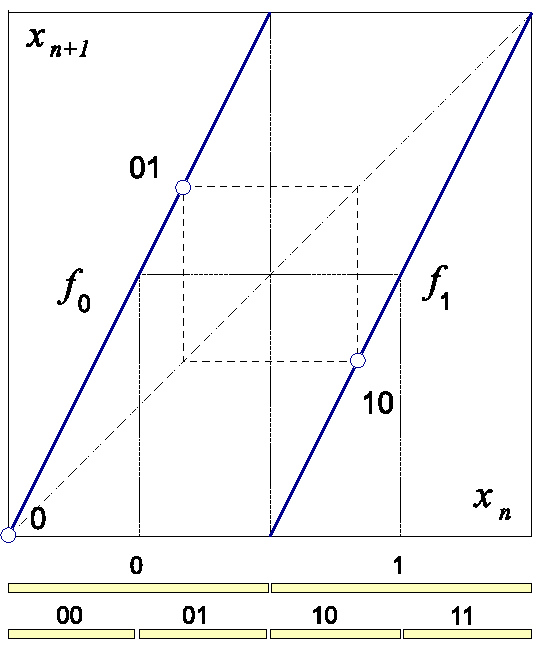
\includegraphics[width=0.35\textwidth]{BernPartCL18}
~~~
{(b)}$\!\!\!\!$
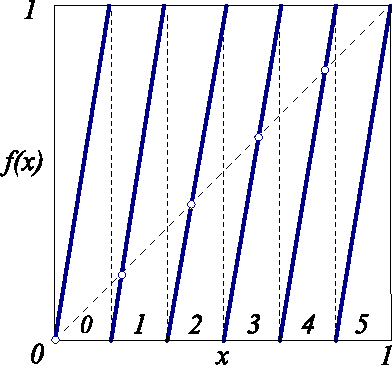
\includegraphics[width=0.40\textwidth]{fig_d_2CL18}

  \caption{\label{fig:BernPart}
(a)
The `coin toss' map \refeq{BerShift}, together with the
$\cycle{0}$ fixed point, and the \cycle{01} 2-cycle. Preimages
of the critical point $\ssp_c=1/2$ partition the unit interval into
$\{\pS_0,\pS_1\}$, $\{\pS_{00},\pS_{01},\pS_{10},\pS_{11}\}$, $\dots$,
subintervals.
(b)
The base-${s}$ Bernoulli map, here with the `dice throw' stretching parameter ${s}=6$,
partitions the unit interval into $6$ subintervals $\{\pS_{\Ssym{}}\}$,
labeled by the ${6}$-letter alphabet \refeq{base-sAlph}. As the map is a
circle map, $\ssp_{5}=1=0=\ssp_{0} \quad(\mbox{mod}\;1)$.
          }
\end{figure}
%%%%%%%%%%%%%%%%%%%%%%%%%%%%%%%%%%%%%%%%%%%%%%%%%%%%%%%%%%%%%%
%

The base-2 {\em Bernoulli} shift map,
\index{Bernoulli!shift}
\index{shift!Bernoulli}
\beq
\ssp_{\zeit+1} =
% \flow{}{\ssp_{\zeit}} =
\left\{ \begin{array}{ll}
        f_0(\ssp_{\zeit}) =  2 \ssp_{\zeit} \,, \quad
                                    & \ssp_{\zeit} \in \pS_0=[0,1/2) \\
        f_1(\ssp_{\zeit}) =  2 \ssp_{\zeit} \;\; (\mbox{mod}\;1)\,, \quad
                                    & \ssp_{\zeit} \in \pS_1 =[1/2,1)
         \end{array}\right.
\,,
\ee{BerShift}
is shown in \reffig{fig:BernPart}\,(a).
If the linear part of such map has an integer-valued slope,
or `stretching' parameter $s\geq2$,
\beq
\ssp_{\zeit+1} \,=\, {s} \ssp_{\zeit}
\ee{BerStretch}
that maps state $\ssp_{\zeit}$ into a state in the `extended \statesp',
outside the unit interval,
the $(\mbox{mod}\;1)$ operation results in the base-${s}$ Bernoulli
circle map,
\renewcommand{\ssp}{\ensuremath{\phi}}             % lattice site field
\beq
\ssp_{\zeit+1}
% = \flow{}{\ssp_{\zeit}}
= {s} \ssp_{\zeit}
\;\; (\mbox{mod}\;1)
%    \,,\qquad \qquad \ssp_{\zeit}\in [0,1)
\,,
\ee{n-tuplingMap}
sketched as a \HREF{https://www.random.org/dice/}{dice throw} in
\reffig{fig:BernPart}\,(b).
The $(\mbox{mod}\;1)$ operation subtracts
$\Ssym{\zeit+1}=\left\lfloor{s}\ssp_{\zeit}\right\rfloor$, the integer part of ${s}
\ssp_{\zeit}$, or the circle map \emph{winding number}, to keep
$\ssp_{\zeit+1}$ in the unit interval $[0,1)$, and partitions the unit
interval into ${s}$ subintervals $\{\pS_\Ssym{}\}$,
\beq
\ssp_{\zeit+1}
% = \flow{}{\ssp_{\zeit}}
% = \hflow{}{\ssp_{\zeit}} - \Ssym{\zeit+1}
= {s} \ssp_{\zeit} - \Ssym{\zeit+1}
\,,\qquad  \ssp_{\zeit}\in\pS_{\Ssym{\zeit}}
\,,
\ee{circ-m}
where $\Ssym{\zeit}$ takes values in the ${s}$-letter alphabet
\beq
\Ssym{} \in \A=\{0,1,2,\cdots,s-1\}
\,.
\ee{base-sAlph}

The Bernoulli map is a highly instructive example of a
hyperbolic dynamical system. Its symbolic dynamics is simple:
the base-${s}$ expansion of the initial point $\ssp_0$ is also its
temporal itinerary, with symbols from alphabet \refeq{base-sAlph}
indicating that at time $\zeit$ the orbit visits the subinterval
$\pS_{\Ssym{\zeit}}$. The map is a `shift':
a multiplication by ${s}$ acts on the base-${s}$
representation of $\ssp_{0}=.\Ssym{1}\Ssym{2}\Ssym{3}\cdots $ (for
example, binary, if ${s}=2$) by shifting its digits,
\bea
\ssp_{1}
    &=& \map(\ssp_{0})
    =.\Ssym{2}\Ssym{3}\cdots
%\continue
%\ssp_{\Ssym{2}\Ssym{3}\cdots}
%    &=& \shift{}\,\ssp_{\Ssym{1}\Ssym{2}\Ssym{3}\cdots}
\,.
\label{shiftBern}
\eea

Periodic points can be counted by observing that the preimages of
critical points $\{\ssp_{c1},\ssp_{c2},\cdots\ssp_{c,s-1}\}$ =
$\{{1}/s,{2}/s,\cdots,(s-1)/s\}$ partition the unit interval into
$\{\pS_0,\pS_1,\cdots,\pS_{s-1}\}$, $\{\pS_{\Ssym{1}\Ssym{2}}\}$, $\dots$,
$s^\cl{}$ subintervals, each containing {\em one}  unstable
period-$\cl{}$ periodic point
$\ssp_{\Ssym{1}\Ssym{2}\cdots\Ssym{\cl{}}}$, with stability multiplier
${s}^\cl{}$, see \reffig{fig:BernPart}. The Bernoulli map is a
full shift, in the sense that every itinerary is \admissible, with one
exception: on the circle, the rightmost fixed point is the same as the
fixed point at the origin, $\ssp_{s-1}=\ssp_{0}\quad(\mbox{mod}\;1)$,
so these fixed points are identified and counted as one, see
\reffig{fig:BernPart}. The total number of periodic points of period
$\cl{}$ is thus
\beq
N_{\cl{}} = s^{\cl{}} - 1
\,.
\ee{noPerPtsBm}


\subsection{Temporal Bernuolli}
\label{s:1D1dLatt}

To motivate our formulation of a \spt\ chaotic field theory to be
developed below, we now recast the local initial value, time-evolution
Bernoulli map problem as a \emph{temporal lattice} fixed point condition,
the problem of enumerating and determining all global solutions.

`Temporal' here refers to the state (field) $\ssp_\zeit$, and the
winding number (source) $\Ssym{\zeit}$ taking their values on the lattice
sites of a 1\dmn\ \emph{temporal}  lattice $\zeit\in\integers$. Over a
finite lattice segment, these can be written compactly  as a
\emph{lattice state} and the corresponding \emph{symbol \brick}
\beq
\transp{\Xx} % = \{\ssp_j\}
             = (\ssp_{\zeit+1},\cdots,\ssp_{\zeit+\cl{}})
\,,\quad
\transp{\Mm} % = \{\Ssym{j}\}
             = (\Ssym{{\zeit+1}},\cdots,\Ssym{{\zeit+\cl{}}})
\,,
\ee{pathBern}
where $\transp{(\cdots)}$ denotes a transpose.
The Bernoulli equation \refeq{circ-m}, rewritten as a first-order
difference equation
\beq
\ssp_{\zeit} - {s}\ssp_{\zeit-1} = - \Ssym{\zeit}
\,,\qquad  \ssp_{\zeit} \in [0,1)
\,,
\ee{1stepDiffEq}
takes the matrix form
\beq
\jMorb\,\Xx = - \Mm
\,,\qquad
\jMorb = \unit-{s}{\hopMat}^{-1}
% former \ee{tempBernFix}
\,,
\ee{tempBern}
where the $[\cl{}\!\times\!\cl{}]$ matrix
\beq
\hopMat_{jk}=\delta_{j+1,k}
\,,\qquad
\hopMat
=  \left(\begin{array}{ccccc}
             0    &  1    &        &   &  \cr
                  &  0    &   1    &   &  \cr
                  &       &        & \ddots &  \cr
                  &       &        & 0 & 1 \cr
             1    &       &        &   & 0
          \end{array} \right)
\,,
\ee{hopMatrix}
implements the shift operation \refeq{shiftBern}, a cyclic permutation
that translates forward in time the lattice state $\Xx$ by one site,
$\transp{(\hopMat \Xx)}=(\ssp_2,\ssp_3,\cdots,\ssp_\cl{},\ssp_1)$. The
time evolution law \refeq{circ-m} must be of the same form for all times,
so the {\shiftOp} $\hopMat$ has to be time-translation invariant, with
$\hopMat_{\cl{}+1,\cl{}}=\hopMat_{1\cl{}}=1$ matrix element enforcing the
periodicity. After $\cl{}$ shifts, a lattice state returns to the initial
state,
\beq
\hopMat^\cl{}=\unit
\,.
\ee{shift2n}

As the {temporal Bernoulli} condition \refeq{tempBern} is a linear
relation, a given \brick\ $\Mm$, or `code' in terms of alphabet
\refeq{base-sAlph}, corresponds to a unique temporal lattice state $\Xx$.
That is why Percival and Vivaldi\rf{PerViv} refer to such symbol \brick\
$\Mm$ as a {\em linear code}.

\subsection{\JacobianOrb}
\label{s:JacobianOrb}

The {temporal lattice} reformulation gives us deep insights into how to
enumerate and determine all global solutions of such systems.
The {temporal Bernoulli} condition
\refeq{tempBern} can be viewed as a search for zeros of the function
\beq
F[\Xx] = \jMorb\Xx+\Mm = 0
\,,
\ee{tempFixPoint}
with the entire periodic \emph{lattice state} ${\Xx}_{\Mm}$ treated as a
single fixed \emph{point} $(\ssp_1,\ssp_{2},\cdots,\ssp_{\cl{}})$ in the
\cl{}\dmn\ \statesp\ unit hyper-cube $\Xx\in[0,1)^\cl{}$, where
the $[\cl{}\!\times\!\cl{}]$ matrix $\jMorb$ is given by \refeq{tempBern}.

The
$F[\Xx]=0$ fixed point condition \refeq{tempFixPoint} is central to the
theory of {global methods} for finding periodic orbits. Instead of
requiring forward-in-time numerical integrations, in multi-shooting
searches for \po s one discretizes a \po\ into $\cl{}$
segments\rf{auto,GM00aut,ChoGuck99,CvitLanCrete02,lanVar1,DingCvit14,DCTSCD14},
and lists a point for each segment
\beq
\transp{\Xx}=(\ssp_1,\ssp_2,\cdots,\ssp_\cl{})
\,.
\ee{nXdCycle}
Starting with an initial guess for \Xx, the zero of function
\refeq{tempFixPoint} is then found by Newton iteration, which requires
an evaluation of the $[\cl{}\!\times\!\cl{}]$ \emph{\jacobianOrb}
\beq
\jMorb_{ij} =\frac{\delta F[\Xx]_i}{\delta \ssp_j}
\,.
\ee{jacobianOrb}
For the particularly simple, linear case at hand, the {\jacobianOrb}
\refeq{tempBern} is the same for all lattice states of period $\cl{}$.

\subsection{Fundamental fact} %{Integer lattices}
\label{s:bernIntLat}

The {\jacobianOrb} \jMorb\ stretches the \statesp\ unit hyper-cube
$\Xx\in[0,1)^\cl{}$ into the \cl{}\dmn\ {\em \fundPip}, and maps each
periodic point ${\Xx}_{\Mm}$ into an integer lattice $\integers^\cl{}$
site, which is then translated by the winding numbers $\Mm$ into the
origin, in order to satisfy the fixed point condition
\refeq{tempFixPoint}. Hence $N_\cl{}$, the total number of the solutions
of the fixed point condition equals the number of integer lattice points
within the {\fundPip}, a number given by what Baake \etal\rf{BaHePl97}
call the `fundamental fact',
\beq
N_\cl{} = |\Det\jMorb|
\,,
\ee{detBern0}
\ie, fact that the number of integer points in the {\fundPip} is equal to
its volume, or, what we refer to as the `{\HillDet}' below. In two
dimensions this formula is known since 1899 as
\HREF{https://en.wikipedia.org/wiki/Pick\%27s_theorem} {Pick's theorem},
in higher dimensions it was given by Nielsen\rf{Nielsen1920,BBPT75} in
1920, and rederived several times since in different contexts, for
example by Baake \etal\rf{BaHePl97}. For the task at hand,
Barvinok\rf{Barvinok04}
\HREF{http://www.math.lsa.umich.edu/~barvinok/lectures.pdf} {lectures}
offer a clear and simple introduction to integer lattices, and a proof of
\refeq{detBern0}.
% as {theorem 2}.

%%%%%%%%%%%%%%%%%%%%%%%%%%%%%%%%%%%%%%%%%%%%%%%%%%%%%%%%%%%%%%%%%%%%%%%
% BernCyc2Jacob.svg
% derived from CatMapStatesp.svg
\begin{figure}
  \centering
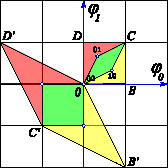
\includegraphics[width=0.35\textwidth]{BernCyc2JacobUnit}
  \caption{\label{fig:BernCyc2Jacob}
The Bernoulli map \refeq{BerShift} periodic points
$\Xx_\Mm=(\ssp_0,\ssp_1)$ of period 2 are the $\cycle{0}=(0,0)$ fixed
point, and the 2-cycle $\Xx_{01}=({1}/{3},{2}/{3})$, see
\reffig{fig:BernPart}\,(a). They all lie within the unit square $[0BCD]$,
which is mapped by the {\jacobianOrb} $\jMorb$ \refeq{bernFundPar} into
the {\fundPip} $[0B'C'D']$. Periodic points $\Xx_\Mm$ are mapped by
$\jMorb$ onto the integer lattice, $\jMorb\Xx_\Mm\in\integers^\cl{}$, and
are sent back into the origin by integer translations $\Mm$, in order to
satisfy the fixed point condition \refeq{tempFixPoint}. Note that this
{\fundPip} is covered by  3 unit area quadrilaterals.
          }
\end{figure}
%%%%%%%%%%%%%%%%%%%%%%%%%%%%%%%%%%%%%%%%%%%%%%%%%%%%%%%%%%%%%%
%
The action of {\jacobianOrb}
$\jMorb$ for the period-2 lattice states (periodic points) of the Bernoulli map of
\reffig{fig:BernPart}\,(a), suffices to convey the idea. In this
case, the $[2\!\times\!2]$ {\jacobianOrb} \refeq{tempBern}, the unit
square basis vectors, and their images are
\bea
\jMorb &=&
 \left(\begin{array}{cc}
  1 & -2 \\
 -2 &  1
 \end{array} \right)
    \continue
\Xx^{(B)} &=&
 \left(\begin{array}{c}
 1  \\
 0
 \end{array} \right)
\;\to\;
\Xx^{(B')} = \jMorb\,\Xx^{(B)} =
 \left(\begin{array}{c}
  1  \\
 -2
 \end{array} \right)
\,,\quad \cdots
\nnu
\eea
\ie, the columns of the {\jacobianOrb} are the edges of the {\fundPip},
\beq
\jMorb = \left(\Xx^{(B')}\Xx^{(D')}\right)
\,,
\ee{bernFundPar}
see \reffig{fig:BernCyc2Jacob}, and $N_2=|\Det\jMorb|=3$,
in agreement with the periodic orbit count \refeq{noPerPtsBm}.

In general, the unit vectors of the \statesp\ unit hyper-cube $\Xx\in[0,1)^\cl{}$
point along the \cl{} axes; \jMorb\ maps them into a {\fundPip} basis
vectors $\Xx^{(j)}$, each one given by a column of the
$[\cl{}\!\times\!\cl{}]$ {\jacobianOrb}
\beq
\jMorb = \left(\Xx^{(1)}\Xx^{(2)}\cdots\Xx^{(\cl{})}\right)
\,.
\ee{lattJac}
The {\HillDet} (discriminant, volume of the {\fundPip}) is
then
\beq
\Det \jMorb = \Det\left(\Xx^{(1)}\Xx^{(2)}\cdots\Xx^{(\cl{})}\right)
\,.
\ee{lattVol}
Note that the unit hypercubes and {\fundPip}s are half-open, as indicated
by dashed lines in \reffig{fig:BernCyc2Jacob}, so that their translates
form a partition of the extended \statesp\ \refeq{BerStretch}.
\refFig{fig:catCycJacob} is another example of a {\fundPip}.

Note that in the {temporal lattice} reformulation, the Bernoulli system
happens to exhibit two unrelated lattices:
\begin{itemize}
  \item[(i)]
In the latticization of a time continuum, one replaces a time-dependent
field $\ssp(\zeit)$ at time $\zeit\in\reals$ of any dynamical system by a
discrete set of its values $\ssp_\zeit=\ssp(\zeit\Delta{T})$,
$\zeit\in\integers$. Here the index $`\zeit'$ is a \emph{coordinate} over
which the field $\ssp$ lives.
  \item[(ii)]
A peculiarity of the Bernoulli system is that the \emph{state}
$\ssp_{\zeit}$ \refeq{n-tuplingMap} is confined to the unit interval
$[0,1)$, imparting a lattice structure onto the calculationally
intermediate, extended \statesp\ \refeq{BerStretch}.
\end{itemize}


\subsection{Counting {temporal Bernoulli} lattice states}
\label{s:bernCount}

To evaluate the {\HillDet} \refeq{detBern0}, observe that
from \refeq{tempBern} it follows that
\[
\Det(-\jMorb)=\Det({s}/\hopMat)\Det(\unit- {\hopMat}/{s})
\,,
\]
where $|\Det({s}/\hopMat)|=s^n$. Expand $\ln\Det(\unit- {\hopMat}/{s}) =
\Tr\ln(\unit- {\hopMat}/{s})$ as a series in $1/s$,
\beq
\Tr\ln\left(\unit- \frac{\hopMat}{s}\right)
  =
-\sum_{k=1}^\infty\frac{1}{k}\frac{\Tr(\hopMat^k)}{s^k}
\,,
\ee{LnDet=TrLn}
and use
$\Tr \hopMat^k= \cl{}\delta_{k,r\cl{}}$
if $k$ is a multiple of $\cl{}$,
0 otherwise
(follows from $\hopMat^\cl{}=\unit$):
\[
\ln\Det(\unit- {\hopMat}/{s})
  =
-\sum_{r=1}^\infty\frac{1}{r}\frac{1}{{s}^{\cl{}r}}
  =
\ln(1-{s}^{-\cl{}})
\,.
\]
So for the {temporal Bernoulli} the volume is
\beq
N_\cl{} = |\Det\jMorb({s})| = {s}^{\cl{}} - 1
\,,
\ee{detBern2n}
in agreement with the time-evolution count \refeq{noPerPtsBm}; all
itineraries are allowed, except that the periodicity of
$\hopMat^\cl{}=\unit$ accounts for $\cycle{0}$ and
$\cycle{s\!-\!1}$ fixed points (see \reffig{fig:BernPart}) being a
single periodic point.


\subsection{Stability of an orbit vs. its time-evolution stability}
\label{s:notHill}

The {\jacobianOrb} $\jMorb_{ij}$ \refeq{jacobianOrb} is a high-\dmn\
linear stability matrix for a {\em zero} of function $F[\Xx_\Mm]=0$,
computed over an entire lattice state $\Xx_\Mm$. How is the `stability' so computed related
to the conventional dynamical systems, forward-in-time stability? To
motivate the answer, consider a temporal lattice with a set of $d$ fields
$\ssp_{\zeit}=\{\ssp_{\zeit,1},\ssp_{\zeit,2},\dots,\ssp_{\zeit,d}\}$ on
each lattice site $\zeit$, and time evolution given by a $d$-\dmn\ map
$\ssp_{\zeit+1}=\map(\ssp_{\zeit})$. The 1-time step $[d\times{d}]$
\jacobianM\ of this dynamical system is
\beq
\jMps(\ssp_{\zeit})_{ij}
=
\left.\frac{\partial \map(\ssp)_i}{\partial \ssp_{j}}\right|_{\ssp_{i}=\ssp_{\zeit,i}}
\,.
\ee{d-1stepJac}
        \PC{2020-02-16}{
Recheck - is this called something like `characteristic function' in
integer lattice and other lattice literature?
    }
Bernoulli systems stretch uniformly, so for the example at hand it
suffices to consider the case of a \jacobianM\ not depending on the field
value $\ssp_{\zeit}$ or time $\zeit$, $\jMps(\ssp_{\zeit}) = \jMps$. For
a $\cl{}$-periodic lattice state $\Xx_\Mm$, the \jacobianOrb\
\refeq{jacobianOrb} is now a $[\cl{}d\times\cl{}d]$ matrix function of the
$[d\!\times\!d]$ block matrix $\jMps$,
\beq
\begin{array}{cc}
 \\ \\ \jMorb(\jMps) & = \\ \\
\end{array}
\left(
\begin{array}{ccccc}
\matId &        & & & -\jMps \\
-\jMps & \matId & \\
       & -\jMps &  \ddots  \\
       &        &   & \matId \\
       &        &   &-\jMps & \matId
\end{array}
\right)
\,,
\ee{dDmnForwardJacobian}
where \matId\ is a $d$-\dmn\ identity matrix.

The evaluation of the {\HillDet} of this more general \jacobianOrb\
proceeds as in the Bernoulli case, the only difference being that the
Bernoulli {\HillDet} is replaced by a function of a matrix,
$\Det\jMorb({s})\to\Det\jMorb(\jMps)$, resulting in \refeq{detBern2n}
being replaced by $|\Det\jMorb(\jMps)|= |\det(\unit-\jMps_\Mm)|$.
    \PC{2020-01-26}{
Insert the \refeq{LnDet=TrLn} step
\beq
\Tr\ln\left(\unit- \frac{\hopMat}{\jMps}\right)
  =
-\sum_{k=1}^\infty\frac{1}{k}{\Tr(\hopMat^k)}{\tr(\jMps^{-k})}
\,,
\nnu\eeq %\ee{LnDetJ=TrLnJ}
    }
Were the 1-step \jacobianM\ $\jMps_\zeit$ varying with time $\zeit$, by
chain rule the period-$\cl{}$ \jacobianM\ would be of form
$\jMps_\Mm=\prod_{\zeit=1}^{\cl{}}\jMps_\zeit$, so the {\jacobianOrb}
evaluated on a lattice state $\Xx_\Mm$, and the dynamical, forward in
time \jacobianM\ are related by
Hill's formula (see \refsect{s:HillForm}):
\beq
|\Det\jMorb_\Mm|=|\det (\unit-\jMps_\Mm)|
\,.
\ee{detDet}

\subsection{\Po\ theory}
\label{s:PoThe}

How come that a `$\Det$' counts lattice states?

For a general, nonlinear fixed point condition $F[\Xx]=0$, expansion
\refeq{LnDet=TrLn} in terms of traces is a cycle
expansion\rf{inv,AACI,ChaosBook}, with support on \emph{periodic orbits}.
Ozorio de Almeida and Hannay\rf{OzoHan84} were the first to relate the
number of periodic points to a \JacobianM\ generated volume; in 1984 they
used such relation as an illustration of their `principle of uniformity':
``periodic points of an ergodic system, counted with their natural
weighting, are uniformly dense in phase space.'' In \po\
theory\rf{inv,CBgetused} this principle is stated as a
\HREF{http://chaosbook.org/chapters/ChaosBook.pdf\#section.27.4} {flow
conservation} sum rule, a sum over all lattice states $\Mm$ of period $\cl{}$,
\beq
\sum_{|\Mm|=\cl{}}
    \frac{1}{|\det (\unit - \jMps_\Mm)|}
    \;= 1
\,,
\label{H-OdeA_mapsOrb}
\eeq
or, by Hill's formula \refeq{detDet},
\beq
\sum_{|\Mm|=\cl{}}
%\sum_{\ssp_i{\in\mbox{\footnotesize Fix}\map^{\cl{}}}}
    \frac{1}{|\Det\jMorb_\Mm|}
    \;=1
\,.
\label{Det(jMorb)eights}
\eeq
For the Bernoulli system the `natural weighting' takes a particularly
simple form, as the {\HillDet} of the {\jacobianOrb} is the same for all
periodic points of period $\cl{}$, $\Det\jMorb_\Mm=\Det\jMorb$, whose
number is thus given by \refeq{detBern0}. Furthermore, for piece-wise
linear systems all curvature corrections\rf{CBcount} for orbits of
periods $k>\cl{}$ vanish, leading to explicit lattice state-counting
formulas reported here.

\subsection{Shadowing}
\label{s:bernShadow}
%        \PC{2020-01-30}{
% link to \templatt\ Green's function \refeq{1dLatGreenFct}
%        }

As the {temporal Bernoulli} condition \refeq{tempBern} is a linear
relation, a given \brick\ $\Mm$, or `code' in terms of alphabet
\refeq{base-sAlph}, corresponds to a unique temporal lattice state $\Xx$
given by the lattice Green's function
\beq
\Xx_\Mm
= \gd\,\Mm
\,,\qquad
\gd = \frac{\hopMat/{s}}{\unit- {\hopMat}/{s}}
\,.
\ee{tempBernGreen}
For an infinite lattice $\zeit\in\integers$, the temporal lattice Green's
function \refeq{tempBernGreen} can be expanded as a series in
$\ExpaEig^{-k}$,
\beq
\gd
    = \frac{\,{\hopMat}/{\ExpaEig}}{\unit-{\hopMat/}{\ExpaEig}}
    = \sum_{k=1}^\infty \frac{\hopMat^k}{\ExpaEig^{k}}
\,,
\ee{BernGreenF}
where $\ExpaEig={s}$ is the 1-time step stability multiplier for the
Bernoulli system. The influence of a source $\Ssym{\zeit'}$ back in the
past, at site $\zeit'$, falls off exponentially with the temporal lattice
distance $\zeit-\zeit'$,
\beq
  \ssp_{\zeit}=\sum_{\zeit'=-\infty}^{\zeit-1} g_{\zeit\zeit'} \Ssym{\zeit'}
\,, \quad
g_{\zeit\zeit'}
   =
   \frac{1}{\ExpaEig^{\zeit-\zeit'}}
\,,\quad \zeit>\zeit'\,,\quad  0\mbox{ otherwise}
\,.
\ee{BernGreenSites}
That means that an ergodic lattice state segment of length \cl{}\ (or a
periodic {lattice state} of a longer period) is shadowed by the periodic
{lattice state} \refeq{pathBern} with the same \cl{}-sites {symbol
\brick} $\Mm$,
    \PC{2020-02-16}{
Do I need to derive this?
    }
\beq
\ssp_{\zeit}
=  \frac{1}{1-1/\ExpaEig^{\cl{}}}
\left(\frac{\Ssym{1}}{\ExpaEig}+\frac{\Ssym{2}}{\ExpaEig^{2}}
      +\cdots
      +\frac{\Ssym{\cl{}-1}}{\ExpaEig^{\cl{}-1}}+\frac{\Ssym{\cl{}}}{\ExpaEig^{\cl{}}}
\right)
,
\label{Bern_cyc}
\eeq
with exponentially
decreasing shadowing error of order $O(1/\ExpaEig^{\cl{}+1})$. The error
is controlled by the \refeq{detDet} prefactor
\(
1/|\Det\jMorb| = 1/|\det(\unit - \jMps_\Mm)|\,,
\)
with the determinant arising from inverting the {\jacobianOrb}
$\jMorb$ to obtain the Green's function \refeq{tempBern}.

This error estimate is deeper than what it might seem at the first
glance. In fluid dynamics, pattern recognition, neuroscience and other
high or $\infty$-dimensional settings distances between `close solutions'
(let's say pixel images of two faces in a face recognition code) are
almost always measured using some arbitrary yardstick, let's say a
Euclidean $L_2$ norm,
even though the state space that has no Euclidean symmetry.
Not so in the \po\ theory: here $1/|\Det\jMorb|$ is the \emph{intrinsic,
coordinatization and norm independent} measure of the distance between
similar \spt\ states.

\subsection{\Tzeta}
\label{s:bernZeta}

Now that we have the numbers of lattice states $N_{\cl{}}$ for any
period $\cl{}$, we can combine them all into a single generating function by
substituting $N_{\cl{}}$ into the {\em topological} or {\em Artin-Mazur}
zeta func\-tion\rf{ArtMaz65,CBcount},
\index{topological!zeta function}
\index{zeta function!topological}
\index{Artin-Mazur zeta function}
\index{zeta function!Artin-Mazur}
    \PC{2020-02-16}{
Do I need to derive this, rather than refer to ChaosBook?
    }
\beq
\zetatop(z) =
     \exp\left(-\sum_{\cl{}=1}^\infty
\frac{z^\cl{}}{\cl{}} N_\cl{}
         \right)
\,,
\ee{topoZeta}
which, when expanded as a Taylor series in $z$, is built from
\emph{primitive} (or \emph{prime}), \ie, non-repeating lattice
states\rf{inv}. Coversely, given the \tzeta, the number of periodic
points of period $\cl{}$ is given by the logarithmic derivative of the
{\tzeta} (see
\HREF{http://chaosbook.org/chapters/ChaosBook.pdf\#section.18.7}
{ChaosBook}\rf{CBcount})
\bea
\sum_{\cl{}=1}N_\cl{} z^\cl{}
    &=& - \,\frac{1}{\zetatop}\,z\frac {d}{dz} (\zetatop)
\,.
\label{zetatop-N}
\eea

For a Bernoulli system \refeq{detBern2n},
\bea
\zetatop(z)
 &=&  \exp \left(-\sum_{\cl{}=1}^\infty
\frac{z^\cl{}}{\cl{}} ({s}^\cl{} - 1)
         \right)
\,=\,
\exp \left[\ln(1 -  {s}z) - \ln(1 - z) \right]
\continue
 &=&
\frac{1 -  {s}z}{1 - z}
\,.
\label{BernZeta}
\eea
The numerator $(1 - {s}z)$ says that a Bernoulli system is a full
shift\rf{CBcount}: there are $s$ fundamental lattice states, in this case
fixed points $\{\ssp_0,\ssp_1,\cdots,\ssp_{s-1}\}$, and every other
lattice state is built from their concatenations and repeats. The
denominator $(1 - z)$ compensates for the single overcounted lattice
state, the fixed point $\ssp_{{s}-1}=\ssp_{0}$ $(\mbox{mod}\;1)$ of
\reffig{fig:BernPart} and its repeats.

\subsection{Counting {temporal Bernoulli} prime \po s}
\label{s:bernPrime}

Substituting the Bernoulli map \tzeta\ \refeq{BernZeta}
into \refeq{zetatop-N}
we obtain
% ------------------- siminos/mathematica/ ----------
% CatMaptopZeta.nb                                    2020-01-18
% Bernoulli map periodic points counting for CL18.tex
\bea
\sum_{n=1}N_n z^n
    &=&
 z+3 z^2+7 z^3+15 z^4+31 z^5+63 z^6+127 z^7
    \ceq
+255 z^8+511 z^9+ 1023z^{10} +2047 z^{11}
\cdots
\,,
\label{bernN_n-s=2}
\eea
in agreement with the lattice states count \refeq{detBern2n}.
The number of \emph{prime} cycles of period $\cl{}$ is given recursively by
subtracting repeats of shorter prime cycles\rf{CBcount},
\beq
M_n\,=\,\frac{1}{n}\left( N_n - \sum _{d|n}^{d<n}\,d M_d \right)
\,,
\ee{primeCount}
where $d$'s are all divisors of $n$, hence
% ------------------- siminos/mathematica/ ----------
% CatMaptopZeta.nb                                    2020-01-18
% Bernoulli map periodic points counting for CL18.tex
\bea
\sum_{n=1}M_n z^n
    &=&
 z+  z^2+2 z^3+3 z^4+6 z^5+9 z^6+18 z^7
    \ceq
+30 z^8+56 z^9+99 z^{10} +186 z^{11}
\cdots
\,,
\label{bernM_n-s=2}
\eea
in agreement with the usual numbers of binary symbolic dynamics prime
cycles\rf{CBcount}.

\subsection{Bernoulli as a continuous time dynamical system}
\label{s:bernODE}

The discrete time derivative of a lattice state \Xx\ evaluated at the
lattice site \zeit\ is given by the \emph{difference operator}\rf{Elaydi05}
    \index{lattice!derivative}\index{derivative, lattice}
    \index{lattice!derivative, forward}\index{difference operator}
\beq
\dot{\Xx}_\zeit =
\left[\frac{\partial\Xx}{\partial\zeit}\right]_\zeit
        =
    \frac{\ssp_{\zeit} - \ssp_{\zeit-1}}{\Delta\zeit}
\ee{lattTimeDer}
The {temporal Bernoulli} condition \refeq{1stepDiffEq} can be thus viewed
as a time-discretized, first-order ODE dynamical system
\beq
   \dot{\Xx} \,=\, \vel(\Xx) \,,
\ee{1stepVecEq}
where the `velocity' vector field $\vel$ is given by
\[
\vel(\Xx) \,=\,
   % \vel(\Xx;\Mm) \,=\,
(s-1)\,\hopMat^{-1}\,\Xx-\Mm
\,,
\]
with the time increment set to $\Delta\zeit=1$, and perturbations that
decay (or grow) with rate $({s}-1)$. By inspection of
\reffig{fig:BernPart}\,(a), it is clear that for \emph{shrinking},
${s}<1$  parameter values the orbit is stable forward in time, with a
single linear branch, 1-letter alphabet $\A=\{0\}$, and the only periodic
lattice states being the single fixed point  $\ssp_0=0$, and its repeats
$\Xx=(0,0,\cdots,0)$. However, for \emph{stretching},  ${s}>1$  parameter
values Bernoulli systems that we study here, every periodic lattice state
$\Xx_\Mm$ is unstable, and there is a \po\ solution for each symbol
\brick\ \Mm.

As far as the time-evolution stability is concerned, the
$|\Det\jMorb_\Mm|=|\det (\unit-\jMps_\Mm)|$ formula \refeq{detDet} is
correct for all first-order difference equations (systems whose evolution
laws are first order in time), for any $[d\times{d}]$ one-time-step
{\jacobianM}. For the Bernoulli system that is a $[1\!\times\!1]$ matrix
$\jMps=s$, with the periodic points count \refeq{detBern2n} trivially
verified.

The {\jacobianOrb} %\refeq{1stepVecEq},
$\jMorb=\partial/\partial\zeit-(s-1)\,\hopMat^{-1}$ is a differential
operator whose determinant one usually computes by a Fourier transform
diagonalization (see \refappe{appe:Fourier}). The Fourier discretization
approach goes all the way back to Hill's 1886 paper\rf{Hill86}; in the
limit of $\cl{}\to\infty$ multi-shooting steps \refeq{nXdCycle}, this is
a remarkable formula, relating a field-theoretic, $\infty$\dmn\
\emph{functional} {\HillDet} $\Det\jMorb_\Mm$ to a determinant of the
finite, $[d\times{d}]$ matrix $\jMps_\Mm$, and it took
\Poincare\rf{Poinc1886} to prove that Hill's Fourier modes calculation is
correct in the continuum limit. Historically,  in \po\ theory
calculations one always computes $\jMps_\Mm$. However, as we shall show
here, and in more generality in \refsect{s:Hill}, it is the {\HillDet}
$\Det\jMorb$ that is the computationally robust quantity that one should
evaluate.

\bigskip

\noindent\textbf{A fair coin toss, summarized.}
We refer to the \emph{global} temporal lattice condition \refeq{tempBern}
as the `\emph{temporal} Bernoulli', in order to distinguish it from the
one-time step Bernoulli evolution \emph{map} \refeq{n-tuplingMap}, in
preparation for the study of \emph{\spt} systems to be undertaken in
\refsect{s:catlatt}. In the lattice formulation, a \emph{global}
{temporally periodic lattice state} $\Xx_\Mm$ is determined by the
requirement that the \emph{local} temporal lattice condition
\refeq{1stepDiffEq} is satisfied at every lattice site. For {temporal
Bernoulli} there is no need for forward-in-time searches for the
returning periodic points. Instead, one determines each global
{temporally periodic lattice state} $\Xx_\Mm$ at one go, by solving the
fixed point condition \refeq{tempFixPoint}, and one determines the total
number of lattice states by computing the {\HillDet} \refeq{detBern0} of
the \emph{\jacobianOrb}. The most importantly for what follows, this
calculation requires no recourse to any \emph{explicit coordinatization
of system's state space} (as, for example, the \AW\ partition of
\reffig{fig:PVAdlerWeiss} below), and \emph{no explicit symbolic
dynamics}.
This is the `\po\ theory'. And if you don't know,
\HREF{https://www.youtube.com/watch?v=_JZom_gVfuw} {now you know}.

The observation that a Bernoulli system can be viewed as a discretization
of a first-order in time ODE, eq.~\refeq{1stepVecEq}, with solutions
whose temporal global linear stability is described by the {\jacobianOrb}
$\jMorb_{ij}=\delta{F[\Xx]}_i/\delta\ssp_j$, has profound implications
for dissipative \spt\ systems such as Navier-Stokes and
Kuramoto-Sivashinsky\rf{GuBuCv17}. However, the goal here is to formulate
a classical {\spt}ly chaotic field theory, Hamiltonian and energy
conserving, because (a) that is physics, and (b) cannot do quantum theory
without it. We need a system as simple as the Bernoulli map, but
mechanical. So, we move on from running in circles, to a mechanical rotor
to kick.

%%%%%%%%%%%%%%%%%%%%%%%%%%%%%%%%%%%%%%%%%%%%%%%%%%%%%%%%%%%%%%%%%%%%%%%
\renewcommand{\statesp}{phase space}
\renewcommand{\Statesp}{Phase space}
\renewcommand{\stateDsp}{phase-space}
\renewcommand{\StateDsp}{Phase-space}

    \ifboyscout\clearpage\fi
% siminos/kittens/cat.tex      pdflatex CL18
% $Author: predrag $ $Date: 2020-08-02 22:02:31 -0500 (Sun, 02 Aug 2020) $

\section{A kicked rotor}
\label{s:kickRot}

The 1-degree of freedom maps that describe kicked rotors
subject to discrete time sequences of angle-dependent impulses
$P(\coord_{\zeit})$, $\zeit\in\integers$,
\bea
\coord_{\zeit+1} &=& \coord_{\zeit}+p_{\zeit+1} \qquad  (\mbox{mod}\;1),
    \label{PerViv2.1b}\\
p_{\zeit+1} &=& p_{\zeit} + P(\coord_{\zeit})
\,,
    \label{PerViv2.1a}
\eea
with $2\pi \coord$ the  angle of the rotor, $p$ the momentum conjugate to
the angular coordinate $\coord$, and the angular pulse
$P(\coord)=P(\coord+1)$ periodic with period $1$, play a key role in the
theory of classical and quantum chaos in  atomic physics, from the
Taylor, Chirikov and Greene  standard map\rf{Lichtenberg92,Chirikov79},
to the cat maps discussed below. The equations are of the canonical
Hamiltonian form: \refeq{PerViv2.1b} is $\dot{\coord}=p/m$ in terms of
discrete time derivative \refeq{lattTimeDer}, \ie, the configuration
trajectory starting at $\coord_{\zeit}$ reaches
$\coord_{\zeit+1}=\coord_{\zeit}+p_{\zeit+1}\Delta{\zeit}/m$ in one time
step $\Delta{\zeit}$, and \refeq{PerViv2.1a} is the time-discretized
$\dot{p}=-\partial V(\coord)/\partial \coord$: at each kick the angular
momentum $p_{\zeit}$ is accelerated to $p_{\zeit+1}$ by the force pulse
$P(\coord_{\zeit})\Delta{\zeit}$, with the time step set to
$\Delta{\zeit}=1$, and the rotor mass $m$ set to 1.

For an atomic physics kicked rotor, the values of the angle $\coord$
differing by integers are identified, but the momentum $p$ is unbounded.
As for the Bernoulli map \refeq{BerStretch}, one compactifies the
momentum by adding $(\mbox{mod}\;1)$ to \refeq{PerViv2.1a}. This reduces
the phase space to a square $[0,1)\times [0,1)$ of unit area, with the
opposite edges identified.

%\section{Life of a single Hamiltonian cat}
\subsection{Cat map}
%    \fi
\label{s:catPV}

The simplest kicked rotor is subject to
a force is proportional to displacement, that is, Hooke's law
force
$P(\coord)=K\coord$ linear in the angular displacement $\coord$. The
$(\mbox{mod}\;1)$ added to \refeq{PerViv2.1a} makes the map a
discontinuous `sawtooth,' unless $K$ is an integer. In the integer $K$ case, the map
(\ref{PerViv2.1b},\ref{PerViv2.1a}) is of form
 \beq
 \left(\begin{array}{c}
 \coord_{\zeit+1}  \\
   p_{\zeit+1}
  \end{array} \right )=
  \jMps \left(\begin{array}{c}
 \coord_{\zeit}  \\
   p_{\zeit}
  \end{array} \right )\quad (\mbox{mod}\;1)
    \,,  \qquad
 {\jMps} =\left(\begin{array}{cc}
 a & c \\
 d & b
  \end{array} \right)
\,,
\ee{catMap}
where $a,b,c,d$ are integers whose precise values do not matter, as long
as $\det \jMps=1$, \ie, the map is area-preserving. The map is then a
Continuous Automorphism of the Torus, or a {\em `cat map'}, a linear
area-preserving map on the unit 2-torus \statesp, with the field at the
temporal lattice site \zeit,
\(
\ssp_{\zeit} =(\coord_{\zeit},p_{\zeit}) \in  (0,1]\times(0,1]
\)
interpreted as the angular position and its conjugate momentum
at time instant $\zeit$.
    \PC{2020-02-20}{
A matrix $\jMps$  is called hyperbolic when it has no eigenvalue on the unit circle.
    }

We consider the case of stability multipliers
$(\ExpaEig\,,\;\ExpaEig^{-1})$ real, with a positive Lyapunov exponent
$\Lyap >0$,
\beq
\ExpaEig=e^{\Lyap}=(s+\sqrt{(s-2)(s+2)})/2
\,,\qquad
s=\tr{\jMps}=\ExpaEig+\ExpaEig^{-1}
\,.
\ee{StabMtlpr}
The eigenvalues are functions of the single stretching parameter $s$, and
for $|s| > 2$ the cat map \refeq{catMap} is a fully chaotic
Hamiltonian dynamical system. Cat maps with the same $s$ are equivalent
up to a similarity transformation, so it suffices to work out a single
convenient realization, as we shall do here for the \PV\ example
\refeq{eq:StateSpCatMap}.

Cat maps are beloved by ergodicists and statistical mechanicians because,
even though the field $(\coord_{\zeit},p_{\zeit})$ is 2\dmn, for integer
values of the stretching parameter $s$, a cat map has a finite alphabet
linear code, just like the Bernoulli map, and its
unit torus can be tiled by two rectangles (see \reffig{fig:PVAdlerWeiss}\,(a)),
in analogy with the forward-in-time Bernoulli map subinterval
partitioning of \reffig{fig:BernPart}. From this it follows that all
admissible symbol {\brick}s can be generated as shifts of finite
type, and all periodic points determined and counted.

As all that is well known, and a side issue for this paper, we relegate
the details of the Hamiltonian cat map dynamics and \po\ counting to
\refappe{s:catMapHam}. Here we focus on reformulating the cat dynamics as
a temporal lattice (or discrete Lagrangian) problem, as we have done for
the Bernoulli system in \refsect{s:1D1dLatt}.

\subsection{\tempLatt}
\label{s:catLagrange}
    % earlier names:
    % \section{Life of a single Lagrangian cat}
    % \section{Cat map in Lagrangian formulation}
\renewcommand{\period}[1]{{\ensuremath{n_{#1}}}}
    % discrete length of a cycle, Predrag

To motivate our formulation of a \spt\ chaotic field theory to be
developed in \refsect{s:catlatt}, we again recast the local initial
value, time-evolution cat \emph{map} \refeq{catMap} as a global
\emph{temporal lattice} condition that we shall refer to as the
{\em \templatt}.

The discrete time Hamilton's equations
(\ref{PerViv2.1b},\ref{PerViv2.1a}) induce forward-in-time evolution on a
2-torus  $(\coord_{\zeit},p_\zeit)$ {\em phase space}. For the problem at
hand, it pays to go from the Hamiltonian (configuration, momentum) phase
space formulation to the discrete Lagrangian
$(\ssp_{\zeit-1},\ssp_{\zeit})$ formulation. If the momentum is replaced
by the discrete time velocity,
\beq
(\coord_\zeit,p_\zeit) \to
\left(
    \ssp_{\zeit},\frac{\ssp_{\zeit} - \ssp_{\zeit-1}}{\Delta\zeit}
\right)
%\,,\qquad \Delta\zeit= 1
\,,
\ee{Ham2Lagr}
and the time step set to $\Delta\zeit=1$, a cat map can be brought to the
\PV\ `two-configuration representation'\rf{PerViv}
\beq
 \left(\begin{array}{c}
 \ssp_{\zeit}  \\
 \ssp_{\zeit+1}
 \end{array} \right )=
 \jMps_{PV} \left(\begin{array}{c}
 \ssp_{\zeit-1}  \\
 \ssp_{\zeit}
 \end{array} \right ) %\mbox{ mod } 1
 - \left(\begin{array}{c}
 0  \\
 \Ssym{\zeit}
 \end{array} \right )
 \,,  \qquad
 {\jMps_{PV}} =\left(\begin{array}{cc}
 0 & 1 \\
 -1 & s
 \end{array} \right ),
%\,.
\ee{eq:StateSpCatMap}
with matrix $\jMps_{PV}$ acting on the 2\dmn\ space of successive
configuration points $\transp{(\ssp_{\zeit-1},\ssp_{\zeit})}$. As was
case for the Bernoulli map \refeq{1stepDiffEq}, the cat map
$(\mbox{mod}\;1)$ condition \refeq{catMap} is enforced by integers
$\Ssym{\zeit}\in  \A$, where for a given integer stretching parameter $s$
the alphabet \A\ ranges over $|\A|={s}\!+\!1$ possible values for
$\Ssym{\zeit}$,
\beq
\A=\{\underline{1},0,\dots s\!-\!1\}
\,,
\ee{catAlphabet}
necessary  to keep $\ssp_{\zeit}$ for all times $t$ within the unit
interval $[0,1)$. We find it convenient to have symbol
$\underline{\Ssym{}}_\zeit$ denote $\Ssym{\zeit}$ with the negative sign, \ie,
`$\underline{1}$' stands for symbol `$-1$'.
As for the Bernoulli system, $\Ssym{\zeit}$ can be interpreted as
`winding numbers'\rf{Keating91}, or, as
they shepherd stray points back into the unit torus, as `stabilising
impulses'\rf{PerViv}. Here we shall refer to them as a `code', or, in
the field-theoretical parlance, as `sources'.

Written out as a second-order difference equation, the \PV\ map
\refeq{eq:StateSpCatMap} takes a particularly elegant, {\em \templatt}
form
\beq
\ssp_{\zeit+1}  -  s \, \ssp_{\zeit} + \ssp_{\zeit-1}
    =
-\Ssym{\zeit}
\,,
\ee{catMapNewt}
or,
in terms of a {lattice state} $\Xx$, the corresponding {symbol \brick}
$\Mm$ \refeq{pathBern}, and the $[\cl{}\!\times\!\cl{}]$ {\shiftOp}
$\hopMat$ \refeq{hopMatrix},
\beq
(\hopMat - s\unit + \hopMat^{-1})\,\Xx = -\Mm
\,,
\ee{catTempLatt}
very much like the {temporal Bernoulli} condition \refeq{tempBern}.
`Temporal' again refers to the global lattice state (field) $\Xx$, and
the winding numbers (sources) $\Mm$ taking their values on the lattice
sites of a 1\dmn\ \emph{temporal} lattice $\zeit\in\integers$.

For a finite lattice segment $\Xx$, one needs to specify the boundary
conditions ({\bcs}).
%  for the Green's function \refeq{tempCatGreen}.
The companion article \refref{GHJSC16} tackles the Dirichlet {\bcs}, a
difficult, time-translation symmetry breaking, and from the \po\ theory
perspective, a wholly unnecessary, self-inflicted pain. All that one
needs to solve the {\templatt} is the $\period{}$-periodic,
time-translation invariant {\bcs} used here.
    \PC{2020-02-08}{
Complain about that stupidity clearly both in the intro and in conclusions.
    }


\subsection{\JacobianOrb}
\label{s:tempCatJacobianOrb}

Again, the {temporal lattice} reformulation gives us a different perspective
into how to enumerate and determine global solutions of such systems. The
{\templatt} condition \refeq{catTempLatt} can be viewed as a search for
zeros \refeq{tempFixPoint} of the function
\beq
F[\Xx] = \jMorb\Xx+\Mm = 0
\,,
\ee{tempCatFixPoint}
% refer to \ee{tempFixPoint}
with the entire periodic \emph{lattice state} ${\Xx}_{\Mm}$ treated as a
single fixed \emph{point} $(\ssp_1,\ssp_{2},\cdots,\ssp_{\cl{}})$ in the
\cl{}\dmn\ unit hyper-cube $\Xx\in[0,1)^\cl{}$, where
the $[\cl{}\!\times\!\cl{}]$ {\jacobianOrb} $\jMorb$ is now given by
\beq
\jMorb = \hopMat - s\unit + \hopMat^{-1}
% \,.
\ee{tempCatFix}
a tri-diagonal Toeplitz matrix (constant along each diagonal,
$\jMorb_{k\ell} = j_{k-\ell}$) of circulant form,
\beq
\jMorb %  = \hopMat - s\unit + \hopMat^{-1}
  =
\left(\begin{array}{ccccccc}
 -{s}& 1 & 0 & 0 &\dots &0& 1 \\
 1 &  -{s}& 1 & 0 &\dots &0&0 \\
0 & 1 &  -{s}& 1 &\dots &0 & 0 \\
\vdots & \vdots &\vdots & \vdots & \ddots &\vdots &\vdots\\
0 & 0 & \dots &\dots &\dots  & -{s}& 1 \\
 1 & 0 & \dots &  \dots &\dots& 1 &  -{s}
        \end{array} \right)
\,.
\ee{Hessian}

% PC 2020-07-24 turned the former
% \subsection{Hill's formula:
%           stability of an orbit vs. its time-evolution stability}
% \label{s:tempLattHill}
% (that was here) into a separate section Hill.tex

\subsection{Integer lattices}
\label{s:catIntLat}

As in \refsect{s:bernIntLat}, the {\fundPip} given the stretching of the
\cl{}\dmn\ unit hyper-cube $\Xx\in[0,1)^\cl{}$ by the {\jacobianOrb}
counts periodic lattice states, with the {\admissible} lattice states of
period $\period{}$ constrained to field values within
$0\leq\ssp_\zeit<1$. The {\fundPip} contains images of all periodic
lattice states $\Xx_\Mm$, which are then translated by integer winding
numbers $\Mm$ into the origin, in order to satisfy the fixed point
condition \refeq{tempCatFixPoint}. The total number of periodic lattice
states is again, as for the Bernoulli system \refeq{detBern0}, given by
the `fundamental fact'
\beq
N_\cl{} = |\Det\jMorb|
\,.
\ee{detCat0}

Period-1, or fixed point lattice states are easy to count: the
{\jacobianOrb} is a 1\dmn\ matrix, so it follows from
\refeq{catMapNewt} that
\beq
N_1={s}-2
\,,
\ee{catFundPar1}
        \PC{2020-06-10}{to Han:
    If the alphabet \refeq{catAlphabet} is really $|\A|={s}\!+\!1$
    letters, how come there are only ${s}-2$ fixed point lattice states?
    Where did the extra 3 letters go?
        }
        \HL{2020-06-12}{
        The fixed point lattice states with the other 3 letters are not admissible. The fixed point solution satisfies:
        \[
        ({s}-2)\ssp_\zeit = \Ssym{\zeit} \, .
        \]
        Since $\ssp_\zeit \in [0,1)$, the range of \Ssym{\zeit} is $\Ssym{\zeit} \in [0,s-2)$. So the letter $\underline{1}$, $s-2$ and $s-1$ are not in the admissible range, as the corresponding fields of these 3 letters are $-1/(s-2)$, $1$ and $(s-1)/(s-2)$ respectively.
        }

%%%%%%%%%%%%%%%%%%%%%%%%%%%%%%%%%%%%%%%%%%%%%%%%%%%%%%%%%%%%%
% Predrag 2020-02-08 replaced Han's
% {HLLength2Counting}.pdf by hand-drawn catCyc2Jacob.svg
% Han & PC 2020-02-11
% siminos/figSrc/han/Mathematica/CountingFigure/HLLength3Counting.nb
\begin{figure}
  \centering
(a)~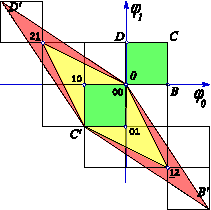
\includegraphics[width=0.38\textwidth]{catCyc2JacobUnit}
~~~
(b)~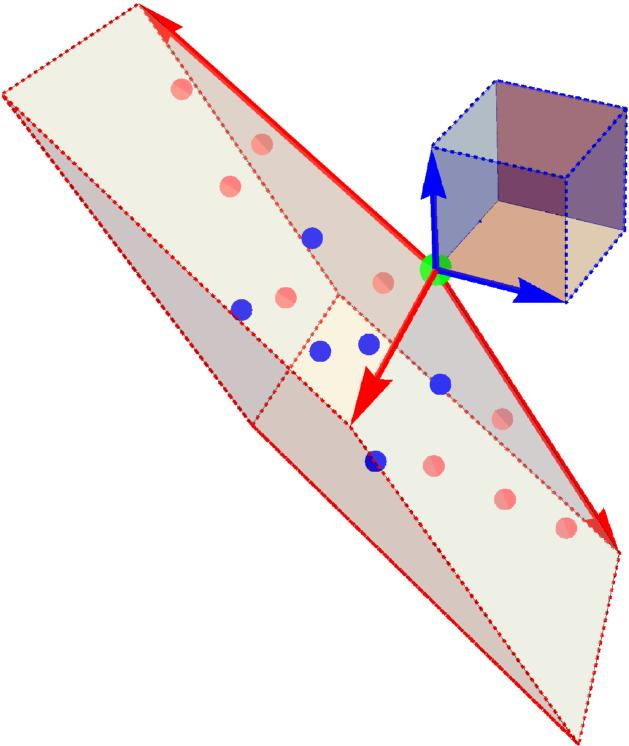
\includegraphics[width=0.34\textwidth]{PCLength3Counting}
  \caption{\label{fig:catCycJacob}
(a)
    For $s=3$, the \templatt\ \refeq{catTempLatt} has 5 period-2 lattice
    states $\Xx_\Mm=(\ssp_0,\ssp_1)$: $\Xx_{00}$ fixed point and
    2-cycles $\{\Xx_{01},\Xx_{10}\}$,
    $\{\Xx_{\underline{1}2},\Xx_{2\underline{1}}\}$. They lie
    within the unit square $[0BCD]$, and are mapped by the
    $[2\!\times\!2]$ {\jacobianOrb} $\jMorb$ \refeq{catFundPar2} into the
    {\fundPip} $[0B'C'D']$, as in, for example, Bernoulli
    \reffig{fig:BernCyc2Jacob}. The images of periodic points $\Xx_\Mm$
    land on the integer lattice, and are sent back into the origin by
    integer translations $\Mm= \Ssym{0}\Ssym{1}$, in order to satisfy the
    fixed point condition
    %\refeq{tempCatFixPoint},
    $\jMorb\Xx_\Mm+\Mm=0$.
(b) A 3-dimensional [{\color{blue} blue} basis vectors] unit-cube stretched by
    $\jMorb$ \refeq{catFundPar3} into the [{\color{red} red} basis vectors]
    {\fundPip}. For $s=3$, the \templatt\
    \refeq{catTempLatt} has 16 period-3 lattice states: a $\Xx_{000}$
    fixed point at the vertex at the origin, [{\color{red} pink dots}] 3
    period-3 orbits on the faces of the {\fundPip}, and
    [{\color{blue} blue dots}] 2 period-3 orbits in its interior.
    An \cl{}\dmn\ unit hyper-cube $\Xx\in[0,1)^\cl{}$ and the
    corresponding {\fundPip} are half-open, as indicated
    by dashed lines, so the integer lattice points on the far corners, edges
    and faces do not belong to it.
}
\end{figure}
%%%%%%%%%%%%%%%%%%%%%%%%%%%%%%%%%%%%%%%%%%%%%%%%%%%%%%%%%%%%%%%

The action of the \templatt\ {\jacobianOrb} is harder to visualize than
the 2\dmn\ {\fundPip} of forward-in-time cat map of
\refappe{s:catHamCount}: a period-2 solution \templatt\ is a 2-torus,
period-3 solution a 3-torus, \etc. Still, the {\fundPip} for the period-2
and period-3 lattice states, \reffig{fig:catCycJacob}, should suffice to
convey the idea. The {\fundPip} basis vectors \refeq{lattJac} are the
columns of $\jMorb$. The $[2\!\times\!2]$ {\jacobianOrb} \refeq{Hessian}
and its {\HillDet} are
\beq
\jMorb =
 \left(\begin{array}{cc}
 -s &  2 \\
  2 & -s
 \end{array} \right)
\,,\qquad
N_2=\Det\jMorb=({s}-2)({s}+2)
\,,
\ee{catFundPar2}
confirming the lattice states count
\refeq{1stChebGenF},
with the resulting {\fundPip} shown in \reffig{fig:catCycJacob}\,(a).
The period-3
lattice states for $s=3$ are contained in the half-open {\fundPip} of
\reffig{fig:catCycJacob}\,(b), defined by the columns of $[3\!\times\!3]$
{\jacobianOrb}
\beq
\jMorb =
\left(
\begin{array}{ccc}
-{s}&  1 &  1 \\
  1 &-{s}&  1 \\
  1 &  1 &-{s}
\end{array}
\right)
\,,
\qquad
N_3 = |\Det \jMorb|
%   = {s}^3-3{s}-2
    = ({s}-2)({s}+1)^2
\,,
\label{catFundPar3}
\eeq
again in agreement with the periodic orbit count \refeq{1stChebGenF}.

The 16 period-3 lattice
states $\Xx_\Mm=(\ssp_0,\ssp_1,\ssp_3)$ are the $\Xx_{000}$ fixed point at the
vertex at the origin, 3 period-3 orbits
    $\{
       \Xx_{\Ssym{0}\Ssym{1}\Ssym{2}},
       \Xx_{\Ssym{1}\Ssym{2}\Ssym{0}}
       \Xx_{\Ssym{2}\Ssym{0}\Ssym{1}}
    \}$
on the faces of the {\fundPip}, and 2 period-3 orbits in its
interior.


\subsection{Counting \templatt\ lattice states (unwritten)}
\label{s:tempCatCount}

We now count the number of periodic lattice states \refeq{noPerPts} in
the \templatt\ (or, `discrete Lagrangian') formulation (for counting
using the Hamiltonian formulation, see \refappe{s:catHamCount}).

[...]
one can write
the {\HillDet} compactly as
\beq
N_\period{} = |\det(\jMorb)|
 = 2\,T_{\period{}}(s/2) -2
% = \ExpaEig^{\period{}} + \ExpaEig^{-\period{}} - 2
\,,
\label{POsChebyshev}
\eeq
Now, use that to simplify the derivation of \refeq{Isola90-13}.
% end of copied from siminos/spatiotemp/chapter/Green1d.tex

\subsection{Counting \templatt\ lattice states (experimental)}
\label{s:tempCatCountTEMP}
% 2020-06-10 Predrag

The \templatt\ equation \refeq{catMapNewt} is
a linear {$2$nd-order inhomogeneous difference} equation
(a $3$-term recurrence relation) with constant coefficients
%\beq
%\ssp_{\zeit+1}  -  s \, \ssp_{\zeit} + \ssp_{\zeit-1}
%    =
%-\Ssym{\zeit}
%%\,.
%\ee{eq:CatMapNewton2}
that can be solved by standard methods\rf{Elaydi05} that
parallel the theory of linear differential equations.
    \PC{2020-06-10}{
    Comparing with \refeq{genFuncts:CatRec-s} we see that we need to
    solve a second-order inhomogeneous difference equation with a
    constant forcing term $2\,(s-2)$.
    }
Inserting a solution of form $\ssp_{\zeit}=\ExpaEig^\zeit$ into the
associated (\Ssym{\zeit}=0) homogenous {$2$nd-order difference equation}
\beq
\ssp_{\zeit+1} - {s}\,\ssp_{\zeit} + \ssp_{\zeit-1}= 0
\ee{diffEqs:CatCharEq}
yields the {characteristic equation}
\beq
\ExpaEig^{2} - {s}\ExpaEig + 1 = 0
\,,
\ee{diffEqs:StabMtlpr}
which, for $|s|>2$, has two real roots
% stability multipliers
$\{\ExpaEig\,,\;\ExpaEig^{-1}\}$,
\beq
\ExpaEig
% =e^{\Lyap}
=\frac{1}{2}(s+\sqrt{(s-2)(s+2)})
\,,
\ee{PCStabMtlpr}
% fundamental solutions \( \{\ExpaEig^\cl{},\ExpaEig^{-\cl{}}\} \),
and the so-called \emph{complementary} solution of form
\beq
\ssp_{c,\zeit}  = a_1\ExpaEig^\zeit+a_{-1}\ExpaEig^{-\zeit}
\,.
\label{PC(2.3.4)}
\eeq
% where constants $a_i$ can be determined by specifying
% $\{\ssp_{0},\ssp_{1}\}$.

A difference of any pair of solutions to the \templatt\
inhomogenous equation \refeq{catMapNewt}
%\beq
%\ssp_{\zeit+1} - {s}\,\ssp_{\zeit} + \ssp_{\zeit-1}= -\Ssym{\zeit}
%%\,,
%\ee{PC(2.4.4)}
is a solution of the homogenous difference equation
\refeq{diffEqs:CatCharEq}, so the general solution is a sum of the
{complementary} solution \refeq{PC(2.3.4)} and a \emph{particular}
solution $\ssp_{p}$,
\beq
\ssp_{\zeit} = \ssp_{c,\zeit} + \ssp_{p,\zeit}
\,.
\ee{PC(2.4.3)}
Eq.~\refeq{diffEqs:CatCharEq} is time-reversal invariant,
$\ssp_{\zeit} = \ssp_{-\zeit}$, so $a_1=a_{-1}=a$.
To determine the particular solution, assume that both the source
 $\Ssym{\zeit}=\Ssym{}$
and $\ssp_{p,\zeit}=\ssp_{p}$
 in \refeq{catMapNewt} are site-independent,
\beq
\ssp_{p}  -  s \,\ssp_{p} + \ssp_{p}
    = -\Ssym{}
\,,
\ee{eq:CatMapNewton5}
so
\(
%  2\,\ssp_{p}-s\,\ssp_{p}={M}
%  \quad \to \quad
  \ssp_{p} = \Ssym{}/(s-2)
\,.
\)
Hence the solution is
\beq
\ssp_{\zeit} = \ssp_{c,\zeit} + \ssp_{p,\zeit}
= a\left(\ExpaEig^{\zeit} + \ExpaEig^{-\zeit}\right) + {\Ssym{}}/(s-2)
\,,
\ee{Chen11:1stepDiffSolu}
with $a_i$ determined by fields at two lattice sites,
\[
\ssp_{0}= 2a + {\Ssym{}}/(s-2)
\,,\quad
\ssp_{1}= a\left(\ExpaEig + \ExpaEig^{-1}\right) + {\Ssym{}}/(s-2)
\,,\quad
\,.
\]
\tempLatt\ starts with $N_{0}=0$, and according to \refeq{catFundPar1},
$N_{1}=s-2$, so $a=1$, $\Ssym{}=-2(s-2)$, and the number
of temporal lattice states of period $\cl{}$ is
\beq
N_{\cl{}} =
    \ExpaEig^{\cl{}} + \ExpaEig^{-\cl{}} - 2
\,.
\ee{PC:1stepDiffSolu}

\subsection{Shadowing}
\label{s:tempCatShadow}

As the
relation between the symbol {\brick}s $\Mm$  and the corresponding
lattice states $\Xx_\Mm$ is linear, for $\Mm$ an {\admissible} symbol
\brick, the corresponding lattice state $\Xx_\Mm$ is given by
the Green's function
\beq
\Xx_\Mm
= \gd\,\Mm
\,,\qquad
\gd = \frac{1}{-\hopMat + s\unit - \hopMat^{-1}}
\,,
\ee{tempCatGreen}
as in the Bernoulli case \refeq{tempBernGreen}.

As in \refsect{s:bernShadow}, the Green's function \refeq{tempCatGreen}
decays exponentially  with the distance from the origin, a fact that is
essential in establishing the `shadowing' between lattice states sharing
a common sub-\brick\ \Mm. For an infinite temporal lattice
$\zeit\in\integers$, the lattice field at site $\zeit$ is determined by
the sources $\Ssym{\zeit'}$ at all sites ${\zeit'}$, by the  Green's function
$g_{\zeit\zeit'}$ for one\dmn\ discretized heat
equation\rf{PerViv,varcyc},
\beq
  \ssp_{\zeit}=\sum_{\zeit'=-\infty}^\infty g_{\zeit\zeit'} \Ssym{\zeit'}
\,, \qquad
%  g_{\zeit\zeit'} =
%       \left(\frac{1}{-\Box -2 +s}\right)_{\zeit\zeit'}
g_{\zeit\zeit'}=\frac{1}{\ExpaEig-\ExpaEig^{-1}}\,
                \frac{1}{\ExpaEig^{|\zeit-\zeit'|}}
% \,,\qquad
% s=\ExpaEig+\ExpaEig^{-1}
\,,
\ee{1dLatGreenFct}  %{Coord}
with $\ExpaEig$ is the expanding stability
multiplier defined in \refeq{StabMtlpr}.

Suppose there is a non-vanishing point source $\Ssym{0}\neq0$ only at the
present, $\zeit'=0$ temporal lattice site. Its contribution to
$\ssp_{\zeit}$ $\sim \ExpaEig^{-|\zeit|}$ decays exponentially  with the
distance from the origin. More generally, as in the Bernoulli case
\refeq{Bern_cyc}, if two lattice states $\Xx$, $\Xx'$ share a common
sub-\brick\ \Mm\ of length \cl{}, they shadow each other with accuracy of
order of $O(1/\ExpaEig^{\cl{}})$.

\subsection{\Tzeta}
\label{s:tempCatZeta}

The number of lattice states of period $\cl{}$ is
given by the area of this {\fundPip}
%\rf{Isola90,Keating91}
\beq
N_{\cl{}} = |\det(\jMps^{\cl{}} - \matId)|
          = \ExpaEig^{\cl{}} + \ExpaEig^{-\cl{}} - 2
\,,
\ee{noPerPts}
where the $\ExpaEig$ is the stability multiplier \refeq{StabMtlpr} of the
one-time-step evolution matrix $\jMps$ \refeq{catMap}.

Substituting the numbers of periodic points $N_{\cl{}}$ into the {\em {\tzeta}} \refeq{topoZeta} we obtain
\index{topological!zeta function}
\index{zeta function!topological}
\index{Artin-Mazur zeta function}
\index{zeta function!Artin-Mazur}
\bea
\zetatop(z)
 &=& \exp \left(-\sum_{\cl{}=1}^\infty
\frac{z^\cl{}}{\cl{}} N_\cl{}
         \right)
 =  \exp \left(-\sum_{\cl{}=1}^\infty
\frac{z^\cl{}}{\cl{}} (\ExpaEig^\cl{} + \ExpaEig^{-\cl{}} - 2)
         \right)
\continue
 &=&
\exp \left[\ln(1 - z \ExpaEig) + \ln(1 - z \ExpaEig^{-1}) - 2 \ln(1 - z) \right]
\continue
 &=&
\frac{(1 - z \ExpaEig)(1 - z \ExpaEig^{-1})}{(1 - z)^2}
 =
\frac{1 - s z + z^2}
     {(1 - z)^2}
\,,
\label{Isola90-13}
\eea
in agreement with Isola\rf{Isola90}, as well as the \AW\ generating
partition \tzeta\ \refeq{Isola90-13a}. As explained in
ChaosBook\rf{CBcount}, \tzeta s count {\em prime} lattice states
\refeq{noPrimeCycs=3}, \ie, the {\em orbits}, \ie, time invariant sets of
periodic points related by cyclic permutations.

In \refeq{POsChebyshev} $T_{\period{}}(s/2)$ is the Chebyshev polynomial
of the first kind, with the generating function \refeq{zetatop-N}
\bea
\sum_{{n}=0}^\infty N_{n} z^{n}
    & = & \frac{2-{s}z}{1 - s z + z^2}-\frac{2}{1 - z}
    \continue
& = & (s-2)\left[z + ({s}+2) z^2 + ({s}+1)^2 z^3 \right.
    \ceq
      \left.+ ({s}+2)\,{s}^2 z^4
      + (s^2+ s-1)^2 z^5 \right.
    \ceq
      \left. +  \cdots\right]
\,,
\label{1stChebGenF}
\eea

\(
s-2,s^2-4,
       s^3-3s-2,
        s^4-4s^2,
        -2 \left(s^3-2s\right)+s\left(s^4-3 s^2+1\right)-2,
\)

\(
        s \left(s^5-4 s^3+3 s\right)-2 \left(s^4-3s^2+1\right)-2,
        -2 \left(s^5-4 s^3+3 s\right)+s \left(s^6-5 s^4+6s^2-1\right)-2,
        %s \left(s^7-6 s^5+10 s^3-4 s\right)-2 \left(s^6-5 s^4+6
%s^2-1\right)-2,-2 \left(s^7-6 s^5+10 s^3-4 s\right)+s \left(s^8-7 s^6+15
%s^4-10 s^2+1\right)-2,s \left(s^9-8 s^7+21 s^5-20 s^3+5 s\right)-2
%\left(s^8-7 s^6+15 s^4-10 s^2+1\right)-2,-2 \left(s^9-8 s^7+21 s^5-20
%s^3+5 s\right)+s \left(s^{10}-9 s^8+28 s^6-35 s^4+15 s^2-1\right)-2,s
%\left(s^{11}-10 s^9+36 s^7-56 s^5+35 s^3-6 s\right)-2 \left(s^{10}-9
%s^8+28 s^6-35 s^4+15 s^2-1\right)-2
\)


\subsection{\tempLatt\ as a continuous time dynamical system}
\label{s:tempCatODE}

Recall how the Bernoulli first-order difference equation could be viewed as
a time-discretization of the first-order linear ODE \refeq{1stepVecEq}. The
second-order difference equation \refeq{catMapNewt} can be interpreted as the
second order discrete time derivative ${d^2}/{dt^2}$, or the temporal
lattice Laplacian,
\beq
\Box \, \ssp_\zeit \equiv
\ssp_{\zeit+1} - 2\ssp_{\zeit} + \ssp_{\zeit-1}
= (s-2)\ssp_{\zeit} -\Ssym{\zeit}
\,,
\ee{PerViv2.2}
 with the time step set to $\Delta\zeit=1$.
But that is nothing but Newton's Second Law: ``acceleration equals
force,'' so Percival and Vivaldi\rf{PerViv} refer to this formulation as
`Newtonian'. We follow Allroth\rf{Allroth83}, Mackay, Meiss, Percival,
Kook \& Dullin\rf{meiss92,MacMei83,MKMP84,DulMei98,kooknewt}, and Li and
Tomsovic\rf{LiTom17b}, in referring to it as the
`Lagrangian' formulation.
%, \refsect{s:catLagrForm}.

In other words, for a cat map the force pulse $P(\coord)=(s-2)\,\coord$
in \refeq{PerViv2.1a} is linear in the angular displacement $\coord$, so
the temporal lattice equation takes form
\beq
(\Box -(s-2)\unit)\,\Xx =-\Mm
%    \,,  \qquad
% \Box\,\ssp_{\zeit}:= \ssp_{\zeit-1}-2\ssp_{\zeit} +\ssp_{\zeit+1}
\,.
\ee{OneCat}
Depending on the value of the real parameter $s$, this equation is known
as either the discrete Helmholtz equation (oscillatory, $s<2$ case), or
-in the case studied here- as the discrete {\em \sPe} (hyperbolic, damped
$s>2$ case)\rf{Dorr70,FetWal03}. Here we shall refer to the discrete
\sPe\ case of \refeq{OneCat} as the `{\em \templatt}', in order to
distinguish it from the forward-in-time Hamiltonian cat \emph{map} \refeq{catMap}.

\PC{2020-07-24} {
    Moved the former subsection {\em Lagrangian formulation}
        % \subsection{Lagrangian formulation}
        % \label{s:catLagrForm}
    (that was here) to blogCats.tex,
    }


\bigskip

\noindent\textbf{\tempLatt, summarized.}
In the \spt\ formulation a \emph{global} {temporal lattice state}
\beq
\transp{\Xx} % = \{\ssp_j\}
             = (\ssp_\zeit,\ssp_{\zeit+1},\cdots,\ssp_{\zeit+k})
\ee{path}
is not determined by a forward-in-time `cat map' evolution
\refeq{catMap}, but rather by the fixed point requirement
\refeq{tempCatFixPoint} that the \emph{local}, 3-term discrete temporal
lattice condition \refeq{catMapNewt} is satisfied at every lattice
point. The Lagrangian formulation requires only temporal lattice states
and their actions, replacing the phase space `cat map' \refeq{catMap}
by a `{\templatt}' lattice \refeq{OneCat}. The {\templatt} has no
generating partition analogue of the \AW\ partition for a Hamiltonian cat
map (see \refsect{s:catAW}).

As we have shown here, no funky Hamiltonian \statesp\ partitioning magic
(such as \reffig{fig:PVAdlerWeiss}) is needed to count the periodic
lattice states of a \templatt. Not only are no such partitions needed to
solve the system, but the Lagrangian, temporal 1\dmn\ lattice formulation
is the bridge that takes us from the single cat map \refeq{catMap} to
the higher-\dmn\ coupled infinity ``multi-cat'' \spt\ lattices
\refeq{dDCatsT}.

And did you know that the cute Arnold map is but the very fundamental
{\sPe} in disguise?


\renewcommand{\period}[1]{{\ensuremath{T_{#1}}}}         %continuous cycle period


%\renewcommand{\Ssym}[1]{{\ensuremath{m_{#1}}}}
\renewcommand{\statesp}{state space}
\renewcommand{\Statesp}{State space}
\renewcommand{\stateDsp}{state-space}
\renewcommand{\StateDsp}{State-space}

    \ifboyscout\clearpage\fi
% siminos/kittens/catlatt.tex      pdflatex CL18
% $Author: predrag $ $Date: 2020-09-20 15:02:24 -0500 (Sun, 20 Sep 2020) $

\section{\catLatt} % {Herding cats}  %
\label{s:catlatt}


The \emph{\templatt} of \refsect{s:kickRot}  is a 1\dmn\ example of the simplest
{\spt}ly chaotic, or `turbulent' field theory, the {\em \catlatt} to
which we turn now. \catLatt\ lives on a  $d$\dmn\ discretized spacetime,
a {\spt} $\integers^d$ integer lattice, with a cat map (a `rotor') on
each site, coupled to its nearest neighbors. Another way of visualizing a
\catlatt\ is as a lattice of locally hyperbolic `anti' oscillators, as
opposed to the classical free field theory, with an oscillator at each
site (`Gaussian model'\rf{Kadanoff00,Fradkin13}).

The \templatt\ lives on a $1$\dmn\ temporal integer lattice $\integers$,
with very  simple `tilings'. For every integer temporal period
$\period{}$, we first determine $N_\period{}$, the number of all periodic
\emph{lattice state} ${\Xx}_{\Mm}$ solutions on a tile of length
$\period{}$. However, if $\period{}=m\period{p}$, the $\period{}$-tile
can be tiled by $m$ repeats of a smaller  $\period{p}$-tile, so {some} of
$\period{}$-{\po} {solutions} are repeats of the already determined
shorter $\period{p}$ \emph{prime} solution  $\Xx_p$. Furthermore, due to
the time invariance of the defining equations, there are $\period{p}$
physically equivalent copies of a given solution in the time orbit of
every $\Xx_p$. So all we really have to do is to enumerate $M_\period{}$
{\em prime orbits} of the time-invariance equivalent \po\ solutions,
whose generating function is the analytically elegant {\tzeta}.

For the $d$\dmn\ \catlatt\ the repertoire of periodic tilings is richer.
In $d=2$ and $3$ the basic facts are well known both from
crystallography, and from the number theory of integer lattices. In this
paper we systematically construct and enumerate distinct $d=2$ tilings,
or Bravais lattices $\LTS{}{}{}$, of increasing spacetime periodicities,
and determine $N_{\LTS{}{}{}}$, the number of \emph{doubly periodic
lattice state} solutions, by evaluating the associated {\HillDet}s.
For $d=2$ and higher-dimensional lattices
counting the \spt\ `prime' tilings requires some thought. We
determine $M_{\LTS{}{}{}}$, the numbers of
doubly-periodic prime orbits, invariant under spacetime translations.
% In this paper we do not quotient the $\integers^2$ space group point, or
% discrete symmetries, and
We, however, fail to find an analytic form for the associated
doubly-periodic {\tzeta}.

We start by a
brief review of physical origin of coupled map lattices (CMLs) models.
The impatient reader should proceed directly to the
{\catlatt}, introduced in \refsect{s:catLatt}, and solved in
\refsect{s:catLattCount}.

\subsection{Coupled map lattices}
\label{s:CCMs}

In order to solve a partial differential equation (PDE) on a computer,
one represents it by a finite number
of computational elements. The simplest discretization of a scalar
spacetime field $\ssp(\vec{q},\tau)$ is by specifying its values
$\ssp_{n_1n_2\cdots{n_{d-1}}\zeit}= \ssp(q_n,\tau_t)$ on lattice points
$(\vec{n},t) \in \integers^{d}$. Once spatial and temporal derivatives
are replaced by their discretizations, the PDE is
reduced to dynamics of a coupled map lattice, a spatially extended system
with discrete time, discrete space, and a set of continuous fields
on each site. For many PDEs, CML conceptual advantage is not only numerical,
but also that the technical problems such as existence and uniqueness of
the field theory are regularized away, and the essence of {\spt} chaos is
revealed in a transparent form.

Often one starts out by coupling neighbors harmonically, and
thinks of this starting, free field theory formulation as a spring
mattress\rf{Zee10} to which  weakly coupled nonlinear terms are then
added. Similarly, the conventional CML models, mostly motivated by
discretizations of dissipative PDEs, start out with chaotic on-site
dynamics weakly coupled to neighboring sites, with a strong space-time
asymmetry. An example are the diffusive coupled map lattices introduced by
Kaneko\rf{Kaneko83,Kaneko84}, with time evolution given by
\bea
\ssp_{n, t+1}
    &=&     (1+\epsilon\,\Box) g(\ssp_{n\zeit})
           \continue
    &=&    g(\ssp_{n\zeit}) + \epsilon %\,\frac{1}{2}
            [
            g(\ssp_{n-1,t}) - 2g(\ssp_{n\zeit}) + g(\ssp_{n+1,t})
            ]
\,,
\label{KanekoCML}
\eea
where the individual spatial site's dynamical system $g(x)$ is a 1\dmn\
map, such as the logistic map, coupled to its nearest neighbors by
$\Box$, the spatial version of the Laplacian \refeq{PerViv2.2} for the
discretized second order \emph{spatial} derivative ${d^2}/{dx^2}$ (we
always set the lattice spacing constant equal to unity).

The form of time-step map $g(\ssp_{n\zeit})$ is the same for all times, \ie, the
law of temporal evolution is invariant under the group of  discrete
\emph{time translations}.
Spatially homogenous lattice models also invariant under discrete \emph{space
translations} were studied by Bunimovich and Sinai\rf{BunSin88} in the case
when  $g(\ssp_{n\zeit})$  is a one\dmn\ expanding map.

The observation that for {\spt}ly chaotic systems space and time should
be considered on the same footing goes back to the `chronotopic' program
of Politi and collaborators\rf{LePoTo96, LePoTo97, PoToLe98, GiLePo95}
who, in their studies of propagation of {\spt} disturbances in extended
systems, discovered that the spatial stability analysis can be combined
with the temporal stability analysis, with orbit weights depending
exponentially both on the space and the time variables,
$t_p\propto{e^{-\speriod{}\period{}\lambda_p}}$.
Politi and
Torcini\rf{PolTor92} study of \twots\ of \emph{\spt\ H{\'e}non}, a
(1+1)-spacetime lattice of H{\'e}non maps with solutions periodic
both in space and time is the closest to the present investigation.
They explain why the dependence
of the lattice field at time $\ssp_{t + 1}$ on the two previous time
steps prevents an interpretation of dynamics as the composition of a
local chaotic evolution with a diffusion process \refeq{KanekoCML}.
In the CML tradition, they study the weak coupling regime $\epsilon\approx0$, but note that the
$b=-1$ case could be an interesting example of a nonlinear Hamiltonian
lattice field theory.


\subsection{Hamiltonian coupled map lattices}
\label{s:HCCMs}

For quantum
mechanics and statistical mechanics applications, one needs the dynamics to
be Hamiltonian, motivating models such as coupled standard map
lattice\rf{KanGra87} and
% Hoover and Aoki
$\phi^4$ lattice\rf{HooAok16}.
%,AokKus00a,AokKus00b,HuLiZh00,AokKus02,AokKus03}
%
Lattice recurrence relations\rf{MraRin12} of the type studied below arise
in the Frenkel-Kontorova lattice, Hamiltonian lattice models for
ferromagnetism, many-body quantum chaos\rf{SieRic01,MuHeBrHaAl04,
GutOsi13a,GutOsi13,GutOsi15}, and in discretizations of elliptic PDEs.
% 2019-06-26  Mramor and Rink
%{\em Ghost circles in lattice {Aubry-Mather} theory}, \arXiv{1111.5963}:
% 2016-10-27 Boris:
% M. Sieber and K. Richter\rf{SieRic01},
% S. M\"uller, S. Heusler, P. Braun, F. Haake and A. Altland\rf{MuHeBrHaAl04},
% Gutkin and Osipov\rf{GutOsi13a}, Gutkin and Osipov\rf{GutOsi13}


Pesin and Sinai\rf{PesSin88} were the first to study such lattices, with
chains of coupled Anosov maps.
In order to establish rigorously the desired statistical
properties of coupled map lattices, such as the continuity of their {SRB}
measures, they, and most of the subsequent statistical mechanics literature,
relied on the structural stability of Anosov automorphisms under small
perturbations. For such lattices the neighboring sites have to be coupled
sufficiently weakly (small $\epsilon$ in \refeq{KanekoCML}) so that the site
cat maps could be conjugated to a lattice of uncoupled Anosov automorphisms,
with a finite Markov partition, the key ingredient required for the proofs.

This exploration, as well as the companion paper\rf{GHJSC16} for
Dirichlet \bcs, starts with the study of a coupled $\speriod{}$-body
Hamiltonian system undertaken by Gutkin and Osipov\rf{GutOsi15}. If the
reader wants to quantize an $\speriod{}$-body Hamiltonian system, Gutkin and Osipov
article covers the formalism in depth, so we do not review the
Hamiltonian formulation here.

\subsection{\catLatt}
\label{s:catLatt}

In their paper, Gutkin and Osipov also note that if the single `body'
dynamics is described by a cat map coupled to its nearest spatial
neighbors, and if the spatial coupling strength is taken to be the same
as temporal coupling strength, one obtains a {\spt}ly symmetric 5-term
recurrence relation
\beq
       \ssp_{n,\zeit+1} + \ssp_{n,\zeit-1}
- 2{s} \, \ssp_{n\zeit}
     + \ssp_{n+1,\zeit} + \ssp_{n-1, \zeit}
     = -\Ssym{n\zeit}
\,,
\ee{CatMap2d}
that adds one spatial lattice direction to  the {\templatt} 3-term
recurrence relation \refeq{catMapNewt}. As these equations are
symmetric under interchange of the `space' and the `time' directions,
their temporal and spatial dynamics are strongly coupled, corresponding to $\epsilon
\approx O(1)$ in \refeq{KanekoCML}, in contrast to the traditional
spatially weakly coupled CML\rf{BunSin88}.

Now that we have mastered the {\em \templatt} \refeq{catMapNewt}, a
generalization to the {\em \catlatt} \refeq{CatMap2d} is
immediate. Consider a 1\dmn\ spatial lattice, with field $\ssp_{n\zeit}$
(the angle of a kicked rotor \refeq{PerViv2.1b} at instant $\zeit$) at
\spt\ site $z=(n,\zeit)\in\integers^2$. If each site couples only to its
nearest spatial neighbors $\ssp_{n\pm1,\zeit}$, and if we require
(1) invariance under spatial translations,
(2) invariance under spatial reflections, and
(3) invariance under the space-time exchange,
we arrive at the 2\dmn\ Euclidean lattice difference equations
\refeq{CatMap2d}.

Gutkin and Osipov --for reasons that make sense in context of $\speriod{}$-body
quantum systems-- call this recurrence relation a `non-perturbed coupled
cat map'. A well-established name\rf{Dorr70,FetWal03} for this system is
the `discrete {\sPe}'. We, however, find a `\emph{\catlatt}' more descriptive
for our field-theoretic purposes.
While the generalization of \refeq{CatMap2d} to $d$\dmn\ hypercubic
$\integers^d$ lattice is immediate, it suffices to work out the $d=2$
\catlatt\ in some detail to develop intuition about the general case.

The \catlatt\ equation \refeq{CatMap2d} can
be written compactly as
\beq
\jMorb\,\Xx =-\Mm
\,,\qquad
\jMorb = \hopMat_1+\hopMat_{2}-2{s}\unit+\hopMat_{2}^{-1}+\hopMat_{1}^{-1}
\,,
\ee{catLatt}
where $\hopMat_1, \hopMat_2$ are {\shiftOp}s \refeq{hopMatrix} which
translate the field by one lattice spacing in the spatial, temporal
direction, respectively. The inverses $\hopMat_{i}^{-1}$ translate the
field in the opposite directions.
The \brick\ $\Mm=\{\Ssym{n\zeit}\}$ is composed of symbols from alphabet
\beq
\Ssym{n\zeit}\in\A
\,,\qquad
 \A  =
 \{\underline{3},\underline{2},\underline{1},0,\cdots,2{s}\!-\!2,2{s}\!-\!1\}
\,,
\label{catLatt2d}
\eeq
where symbol $\underline{\Ssym{}}{}_{n\zeit}$ denotes $\Ssym{n\zeit}$ with the
negative sign, \ie, `$\underline{3}$' stands for symbol `$-3$'.
%
In our explicit computational examples, we shall always set ${s}$ to
\beq
{s}=5/2
    \quad\Rightarrow\quad
 \A  =
 \{\underline{3},\underline{2},\underline{1},0,1,2,3,4\}
\,,
\ee{s=5over2}
the smallest value of the `stretching' parameter $s$ for which the
{\jacobianOrb} $\jMorb$ is an integer-valued matrix, and  the system is
hyperbolic.

%Building upon the $d=1$ {\templatt} developed in \refsect{s:catLagrange},

As for the {temporal Bernoulli} \refeq{tempBern} and the
\templatt\ \refeq{tempCatFixPoint}, one can view the
\catlatt\ condition
\refeq{catLatt} as a zero of the function
\beq
F[\Xx] = \jMorb\Xx+\Mm = 0
\,,
\ee{lattFixPoint}
with the entire periodic {lattice state} ${\Xx}_{\Mm}=\{\ssp_z\}$ treated
as a single fixed {point} within the $(\ell_1\ell_2\cdots\ell_d)$\dmn\
unit hyper-cube $\Xx\in[0,1)^{\ell_1\ell_2\cdots\ell_d}$, where $\ell_j$
is the lattice period in direction $j$, and the
$(\ell_1\ell_2\cdots\ell_d)^2$\dmn\ {\jacobianOrb} $\jMorb_{zz'}$ is
given by
\beq
\jMorb = \sum_{j=1}^{d}\left(\hopMat_j-{s}\unit+\hopMat_{j}^{-1}\right)
\,.
\ee{catlattFix}
Here $\hopMat_i$ is a {\shiftOp}
\refeq{hopMatrix} which translates the field in the $i$th
direction by one lattice spacing. Its inverse $\hopMat_{i}^{-1}$
translates the field in the negative $i$th direction.

In multi-index, or `tensorial' notation, the \catlatt\ equation
\refeq{catLatt} can be written as
\bea
\left(\jMorb\ssp\right)_{{z}}
&=&
\sum_{{z}'} \sum_{i=1}^{d} \left(
\hopMat_{i}-{s}\unit+\hopMat_{i}^{-1}
                               \right)_{{z}{z}'}
     \ssp_{{z}'} = - \Ssym{z}
\,,\quad
  \Ssym{z} \in \A
\continue
{z} &=& (n_1,n_2,n_3,\cdots,n_d) \in \integers^d
\continue
\A &=& \{-2d+1, -2d+2,\cdots,2{s}-2,2{s}-1\}
\,,
\label{dDCatsT}
\eea
with field $\ssp_{z}$ and source $\Ssym{z}$ labelled by the $d$ indices
of lattice site $z$.  Sources $\Ssym{z}\in\A$ keep the field (`rotor
angle' $\ssp_{z}$) within the unit interval on every site. The
{\jacobianOrb} $\jMorb$, labelled by $d$ pairs of indices, acts on the
lattice state \Xx\ by usual matrix multiplication. We illustrate how that
works by working out  in detail an example in \refappe{s:catLattRel3x2}.
As yet another notational choice,  in \refeq{catalattLxT} we recast
the \jacobianOrb\ \refeq{catLatt} as a
$[\speriod{}\period{}\times\speriod{}\period{}]$ Kronecker product block
matrix.

%2020-09-05
\subsection{Symmetries of the integer lattice}
\label{s:lattSymm}

The \catlatt\ equation \refeq{catLatt} is \emph{equi}variant under
the discrete spacetime translations;
the space $\sigma_{x}$ and time $\sigma_{y}$ reflections $n\to -n$,
$t\to-t$;
as well as under $\sigma_{a}$ exchange $n\longleftrightarrow t$ of space
and time.
{\catLatt} thus has the point-group symmetries of the square lattice:
rotations by $\pi/2$, and reflection across $x$-axis, $y$-axis, and
diagonals $a$ and $b$,
\beq
C_{4v} = \Dn{4} = \{
E, C_{4z}^+, C_{4z}^-, C_{2z},
\sigma_{y}, \sigma_{x},
\sigma_{a},\sigma_{b},
\}
\,.
\ee{eq:C4v}
In the international crystallographic notation, the square lattice space
group of symmetries is referred to as $p4mm$\rf{Dresselhaus07}.



\subsection{Bravais lattices}
\label{s:BravaisLatt}

For the 1\dmn\ temporal lattices considered so far,
a sublattice is tiled by repeats of a \brick\ of temporal period \period{}.

    \PCedit{ %2020-09-05
For a $d$\dmn\ integer lattice $\integers^d$, a $d$-periodic
sublattice that tiles the spacetime is called a
\emph{Bravais lattice}.
    }

    \HLedit{
For a $d$\dmn\ integer lattice $\integers^d$, the primitive unit cell of
a $d$\dmn\ Bravais lattice tiles the spacetime.
    }

A 2\dmn\ {Bravais lattice} $\Lambda$ is an infinite array of points
\beq
\Lambda = \{n_1 \mathbf{a}_1 + n_2 \mathbf{a}_2\,|\,n_i \in \mathbb{Z}\}
\,,
\ee{2DBravaisLattice}
generated by the group of discrete translations
\(
{R} =n_{1}\mathbf{a}_{1}+n_{2}\mathbf{a}_{2}
\,,
\)
where $\{n_{1},n_{2}\}$ are any integers, and
$(\mathbf{a}_{1},\mathbf{a}_{2})$ is a pair of $\integers^2$ integer
lattice vectors that
% defines a \emph{Bravais cell}, a tile that tiles the Bravais lattice.
	\HLedit{
span the Bravais lattice as a set of basis.

The primitive unit cell of a Bravais lattice can be
chosen in different ways. In this paper we will always choose the primitive unit cell uniquely corresponding
to the basis vectors:
\beq
C(\mathbf{a}_{1},\mathbf{a}_{2}) = \{m_1 \mathbf{a}_1 + m_2 \mathbf{a}_2\,|\, 0 \leq m_i < 1\}
\,,
\ee{2DBravaisCell}
and call $C(\mathbf{a}_{1},\mathbf{a}_{2})$ the \emph{Bravais cell} of Bravais spanned by basis vectors
$(\mathbf{a}_{1},\mathbf{a}_{2})$.
	}

%%%%%%%%%%%%%%%%%%%%%%%%%%%%%%%%%%%%%%%%%%%%%%%%%%%%%%%%%%%%%
% figSrc/han/Mathematica/HLBravaisLattice.nb
% half of Han's \reffig{fig:HLReciprocalLattice}
\begin{figure}
  \centering
%(a)
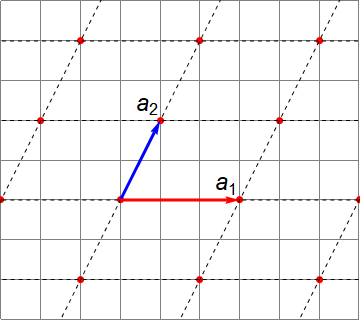
\includegraphics[width=0.40\textwidth]{HLBravaisLattice}
~~~
% (b)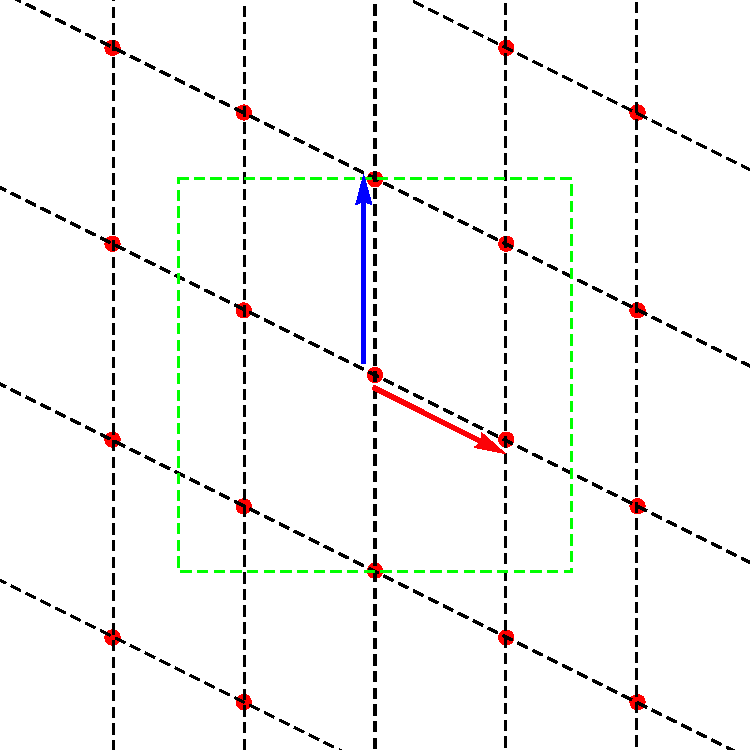
\includegraphics[width=0.40\textwidth]{HLReciprocalLattice1}
  \caption{\label{fig:BravaisLatt}
  (Color online)
%(a)
    The intersections of the (light grey) solid lines form the square
    lattice on which the discrete field $\ssp_z$ is defined. The (red)
    basis vector $\mathbf{a}_1=(3,0)$ and the (blue) basis vector
    $\mathbf{a}_2=(1,2)$ form a $\LTS{}{}{}=\BravCell{3}{2}{1}$ Bravais
    cell. The intersections (red points) of the black dashed lines form
    the Bravais lattice $\Lambda$.
% dropped \reffig{fig:HLReciprocalLattice}\'(b)
}
\end{figure}
%%%%%%%%%%%%%%%%%%%%%%%%%%%%%%%%%%%%%%%%%%%%%%%%%%%%%%%%%%%%%%%

A given Bravais \emph{lattice} $\Lambda$  can be defined by any of the infinity of
Bravais cells,
each defined by a different pair of basis vectors
$(\mathbf{a}_{1},\mathbf{a}_{2})$, but equivalent under unimodular,
\SLn{2}{\integers} transformation\rf{Lang71}.
    \PC{2020-09-05}{
recheck Lang\rf{Lang71} {\em Linear Algebra}, or replace!
It is possible that it does not reference  modular group at all...
    }
Each such family contains a unique
Bravais cell of the \emph{Hermite normal form}\rf{Cohen93}, which, for a
2\dmn\ square lattice, can be chosen to have the first basis vector
pointing in the spatial direction\rf{Lind96}
\beq
\mathbf{a}_1=\left(\begin{array}{c}
  \speriod{}\\
  0{}
  \end{array}\right)
  \,,\qquad
\mathbf{a}_2=\left(\begin{array}{c}
  \tilt{}\\
  \period{}
  \end{array}\right)
  \,,
\ee{Hermite2d}
where $\speriod{}$, $\period{}$ are respectively the spatial, temporal
lattice periods, and the `tilt'\rf{OKKH99} $0\leq\tilt{}<\speriod{}$ imposes the
relative-periodic `shift' {\bcs}\rf{ChaosBook}
(in the integer lattices literature these are also
referred to as
\emph{`helical'}\rf{LHCLL06} vs. \emph{`toroidal'}\rf{IzOgCh02};
\emph{`twisted'} and
\emph{`twisting factor'}\rf{LHCLL06};
\emph{`screw'}
{\bcs}).
We label Bravais cell \refeq{Hermite2d} and the corresponding Bravais
lattice $\Lambda$ by \LTS{}{}{}. An example is the $\BravCell{3}{2}{1}$
Bravais lattice is shown in \reffig{fig:BravaisLatt}.

\PCedit{  %2020-09-05
For each width  $\speriod{}$, height  $\period{}$,
the number of (tilted) Hermite normal form Bravais cells is
\beq
\#_{[\speriod{}\times\period{}]}
   = \sum_{\tilt{}=0}^{\speriod{}-1} 1
   = \speriod{}
\,,
\ee{noBravLatts}
and a Bravais lattices-counting zeta function (see Lind\rf{Lind96}
Example~3.1) can by constructed by substituting
$\#_{[\speriod{}\times\period{}]}$ into
\bea
1/\zeta(z)
 &=& \exp \left(-
 \sum_{\speriod{}=1}^\infty
  \sum_{\period{}=1}^\infty
  \#_{[\speriod{}\times\period{}]}
  \frac{z^{\speriod{}\period{}}}{\speriod{}\period{}}
         \right)
 =  \exp \left(-\sum_{\speriod{}=1}^\infty
                \sum_{\period{}=1}^\infty
    \frac{(z^{\speriod{}})^{\period{}}}{\period{}}
         \right)
\continue
 &=&
   \exp\left(\sum_{\speriod{}=1}^\infty
                \ln(1 - z^{\speriod{}})
         \right)
  =
\prod_{\speriod{}=1}^{\infty}(1 - z^{\speriod{}})
\,.
\label{Lind96Examp3-1}
\eea
    }
    \PC{2020-09-05}{
As long as I do not understand the logic of this zeta function,
we will have to drop it from the paper...
    }


\subsection{Prime Bravais lattices}
\label{s:primeLatt}
% PC{2020-09-05}{ This section was called ``{\em Prime \twots}'' }

It might be possible to tile a given Bravais lattice $\Lambda$
by a finer lattice $\Lambda_p$. Lattice $\Lambda_p$, defined
by a Bravais cell
\beq
\mathbf{a}^p_{1}=\left(\begin{array}{c}
  \speriod{p}\\
  0{}
  \end{array}\right)
  \,,\qquad
\mathbf{a}^p_{2}=\left(\begin{array}{c}
  \tilt{}_{p}\\
  \period{p}
  \end{array}\right)
\,,
\ee{primeTile}
is a \emph{prime} Bravais lattice, if there is no finer Bravais cell,
other than the unit volume $\BravCell{1}{1}{0}$ Bravais cell, that can
tile it.
    \PC{2020-07-15}{
   In \emph{siminos/spatiotemp/chapter/integLatt.tex} Dudgeon and
   Mersereau\rf{DudMer84} explain clearly that if $\det\Lambda$ is a
   prime number, then $\Lambda$ is a \emph{prime matrix}. If $\Lambda$ is
   neither prime nor unimodular, it is \emph{composite}, and can be
   decomposed, nonuniquely - up to a unimodular transformation - into a
   product of two non-unimodular matrices \(\Lambda=PQ\). Then one can
   ``quotient'' $Q$ by ``dividing'' by $P$.
    }

In order to determine all prime lattices $\Lambda_p$ \refeq{primeTile}
% with Bravais cells \( (\mathbf{a}^p_{1},\mathbf{a}^p_{2}) \,, \)
 that tile a given Bravais lattice $\Lambda$ \refeq{Hermite2d},
%with  Bravais cell
%\(
%(\mathbf{a}_1,\mathbf{a}_2)
%\,,
%\)
\bea
\mathbf{a}_1 &=& k\,\mathbf{a}^p_{1} + \ell\,\mathbf{a}^p_{2}
    \continue
\mathbf{a}_2 &=& m\,\mathbf{a}^p_{1} +    n\,\mathbf{a}^p_{2}
\,,
\nnu
\eea
observe that a prime tile
\(
(\mathbf{a}^p_{1},\mathbf{a}^p_{2})
\)
tiles the larger tile only if larger tile's width
$\speriod{}$ is a multiple of $\speriod{p}$, the height
$\period{}$ is a multiple of $\period{p}$, and the two tile `tilts'
satisfy
\[ %beq
\mathbf{a}_2 = {m}\,\mathbf{a}^p_{1} + \frac{\period{}}{\period{p}} \mathbf{a}^p_{2}
\quad\rightarrow\quad
\tilt{} = {m} \speriod{p} + \frac{\period{}}{\period{p}} \tilt{p}
\,.
\] %\ee{primeTiling}
Hence a prime lattice $\Lambda_p$ tiles the given lattice $\Lambda$ only if
the area spanned by the two `tilted' basis vectors
\beq
\mathbf{a}_2\times\mathbf{a}^p_{2}=\tilt{}\period{p}-\period{}\tilt{p}
\ee{primeTiling}
is a multiple of the prime tile area $\speriod{p}\period{p}$.

    \PCedit{ %2016-11-08
\subsection{Lattice states}
\label{s:lattState}

A \emph{lattice state} is a set of all field values $\Xx = \{\ssp_z\}$
over the $d$\dmn\ lattice $z\in\integers^d$ that satisfies the
\catlatt\ equation \refeq{catLatt}, with all field values constrained to
$0\leq\ssp_z<1$.

While the {\catlatt} equation \refeq{catLatt} is \emph{equivariant} under
the integer lattice \emph{space group} $p4mm$ symmetry operations
\refeq{eq:C4v}, the individual lattice states either have no symmetry at
all (they are, after all, `turbulent'), or are invariant under subgroups
of space group $p4mm$.  In what follows we quotient only the translational
symmetries, and postpone dazzling the captive reader with the full \Dn{4}
point group reduction to a later, more ponderous publication.
}

    \PCedit{ %2020-09-05
Furthermore, inspection of the \templatt\
\reffig{fig:catCycJacob} suggests that there is a \emph{field symmetry}
under inversion though the center of the $0\leq\ssp_z<1$ unit interval.
Indeed, if
$\Mm=\{\Ssym{n\zeit}\}$, composed of symbols from alphabet
\refeq{catLatt2d}, corresponds to a 2\dmn\ lattice state
${\Xx}_{\Mm}=\{\ssp_{n\zeit}\}$, its conjugation symmetry partner
\beq
\bar{\Mm}=\{\bar{\Ssym{}}_{n\zeit}\}
\,,\qquad \bar{\Ssym{}}_{n\zeit} =
2(s-2)-\Ssym{n\zeit}
\,,
\ee{Mconjug}
corresponds to lattice state
${\bar{\Xx}}_{\bar{\Mm}}=\{1-\ssp_{n\zeit}\}$. So, every lattice state
either belongs to a conjugate pair
$\{{\Xx}_{\Mm},\bar{\Xx}_{\bar{\Mm}}\}$, or is self-dual under
conjugation.
%  P 2020-09-05 tests: $2s-4-(2{s}\!-\!1)=-3$; $2s-4-(0)=2s-4 \Rightarrow 1$
}

While the action of {\jacobianOrb} $\jMorb$ \refeq{dDCatsT} maps
fields $\ssp_{n\zeit}$ to values outside the unit interval, such values
that are then returned back to the  unit interval by integer
\Ssym{n\zeit}. This `$\integers^1$ lattice action' at every \spt\ lattice site
is a peculiarity of the coupled Bernoulli and cat map lattice models, not
a condition that a \spt\ discretization of a generic field theory would
satisfy, and should never be confused with a discretization of spacetime
continuum to integer lattice $\integers^d$.



For brevity, we shall refer to lattice state $\Xx$ as a
\emph{\twot} if it satisfies
\beq
\Xx({z} + {R}) = \Xx({z})
\ee{dDprimePO}
for any discrete translation
\(
{R} =n_{1}\mathbf{a}_{1}+n_{2}\mathbf{a}_{2}
\in \Lambda
\,,
\)
where $\{n_{1},n_{2}\}$ are any integers, and
$(\mathbf{a}_{1},\mathbf{a}_{2})$ is a pair of $\integers^2$ integer
lattice vectors that define a \emph{Bravais cell}. We shall always refer
to a Bravais sublattice \HLedit{(sublattice of $\integers^2$)} by its unique {Hermite normal form} {Bravais
cell} \refeq{Hermite2d} \HLedit{(basis?)}, and denote it $\Lambda=\LTS{}{}{}$,
a 2\dmn\ doubly-periodic
(relative) \emph{\twot}
\beq
\ssp_{n\zeit} = \ssp_{n + \speriod{}, \zeit}
                 = \ssp_{n+\tilt{}, \zeit+ \period{}}
    \,,\qquad
(n,\zeit)\in\integers^2
\ee{Woods12p6}
with periods $(\speriod{},\period{})$ and tilt $\tilt{}$.

A correct  definition of  a {\em prime} {\twot}\rf{DasBuchMirror} is
subtler than for the 1\dmn\ temporal lattice case. If a given {\twot}
over lattice $\Lambda$ is not periodic under translations
\({R}\in\Lambda_p\) on any sublattice $\Lambda_p$ (except for $\Lambda$
itself), we shall refer to it here as a \emph{prime {\twot}}, a \po\ of
the smallest periodicity in all spacetime directions.
    \PC{2020-09-08}{
The $\integers^d$ unit cell is always one of $\Lambda_p$, see
\reftab{tab:LxTs}, do we say that anywhere?
    }
We return to explicit construction of prime \twots\ in \refsect{s:prime}.
Prime \twots\ are the basic building blocks of \tzeta s (see
\refsect{s:bernZeta} and \ref{s:tempCatZeta}).



Explicitly verifying the periodic lattice states counting formulas for
several 2\dmn\ \catlatt\ examples is now in order.

The simplest examples of {\twots} are
(i) spacetime \eqva\ over $\BravCell{1}{1}{0}$,
(ii) space-\eqva\ over $\BravCell{1}{\period{}}{0}$,
(iii) time-\eqva\  over $\BravCell{\speriod{}}{1}{0}$,
and
(iv) time-\reqva\ over $\BravCell{\speriod{}}{1}{\tilt{}}$,  $\tilt{}\neq0$,
stationary patterns in a time-reference frame\rf{PolTor92} moving with a constant
velocity $\tilt{}/\period{}$.

\subsubsection{Spacetime \eqva\ over $\BravCell{1}{1}{0}$.}
\label{s:catLatt1x1}


\subsubsection{Time-\eqva\ over $\BravCell{\speriod{}}{1}{0}$.}
\label{s:catLattLx1}
Consider the time-\eqv\
\(
\ssp_{n\zeit} = \ssp_{n1}
\)
for all spatial sites $n$, and all times $\zeit$.
To see that this is the 1\dmn\ lattice \templatt\ tiles of period
\speriod\ already counted in \refsect{s:tempCatCount}, note that the 5-term
recurrence relation \refeq{CatMap2d} reduces to the 3-term recurrence
\beq
\ssp_{n+1,1}-2({s}_2-1)\,\ssp_{n1}+\ssp_{n-1,1}
     = -\Ssym{n1}
\,,
\ee{eq:CatLattT=1}
where we have temporarily added index `${}_2$' to the stretching parameter
${s}_2$ to indicate that it refers to the 2\dmn\ \catlatt. Comparing with
the \templatt\ \refeq{catMapNewt},
\(
\ssp_{\zeit+1}  -  {s}_1\, \ssp_{\zeit} + \ssp_{\zeit-1}
    =
-\Ssym{\zeit}
\,,
\)
we see that we have already counted all lattice states on Bravais cells of form
$\BravCell{\speriod{}}{1}{0}$, provided we replace
\(
{s}_1\to2({s}_2-1)
\)
in \refeq{1stChebGenF}. For the values chosen in
our numerical examples,
\( {s}_1=3 \)
and
\( {s}_2=5/2 \,,\)
the two counts happen to be the same and given by \refeq{catMapN_n-s=3}.

However, already the smallest \emph{relative}-periodic
\BravCell{\speriod{}}{1}{\tilt{}}
%$\BravCell{\speriod{}}{1}{0}_\tilt{}$
Bravais lattices are new, and perhaps
surprising.

\subsubsection{Relative  $\BravCell{2}{1}{1}$ \twot.}
\label{s:catLattRel2x1}

% was in siminos/spatiotemp/chapter/CL18blog.tex
% \HLpost{2019-08-08}{
Consider a $\BravCell{2}{1}{1}$ \twot\ with tilt periodic \bcs,
periodic state
\(
\Xx_{\Ssym{1}\Ssym{2}} =
 [
 \begin{array}{cc}
 \ssp_{1} & \ssp_{2}
 \end{array}
 ]
\,,
\)
tiled by the Bravais lattice
\refeq{2DBravaisLattice} with basis vectors $\mathbf{a}_1=\{2,0\}$ and $\mathbf{a}_2=\{1,1\}$, see \reffig{fig:2x1rpo}\,(a).
    \PC{2020-02-23}{
This is wrong, it is written for the symmetric alphabet that we do not use. Fix.
    }	
\beq
\Xx_{\underline{\Ssym{}}\Ssym{}} = \frac{1}{9}
 \left[
 \begin{array}{cc}
 -\Ssym{} & \Ssym{}
 \end{array}
 \right]
        \,,\qquad
\Ssym{}\in\A
         \,,
\ee{catLattRel2x1}
for example
\[
\Mm =
 \left[
 \begin{array}{cc}
 -4 & 4
 \end{array}
 \right]
 \Rightarrow\quad
\Xx_{\underline{4}4} = \frac{1}{9}
 \left[
 \begin{array}{cc}
 -4 & 4
 \end{array}
 \right]
 \,.
\]
Note that these are `periodic lattice state' solutions: there is one \emph{prime}
\twot\ for each set of period-2 periodic lattice states related by cyclic
permutations,
\(
\cycle{\underline{\Ssym{}}\Ssym{}}
    =
(\Xx_{\underline{\Ssym{}}\Ssym{}}, \Xx_{\Ssym{}\underline{\Ssym{}}})
\,,
\)
and there are only 4 of those, as $\Xx_{00}=\Xx_{0}$ is a repeat of the
1-\brick.

By \refeq{2x1_1Fourier} the number of $\BravCell{2}{1}{1}$ relative
\twots\ with the given Bravais lattice bc's is 9.
Using the Green's function method \refeq{GreenFuncCoupled} one can verify
that there are indeed 9 such \twots,
one \twot\ solution for each letter of alphabet \refeq{catLatt2d},

\subsubsection{$\BravCell{2}{1}{0}$ \twot.} %$[2\!\times\!2]$
\label{s:catLatt2cycles}
    %
    %    \HLpost{2019-08-12}{
As an illustration of the {\fundPip} \refeq{detBern0}
%\refeq{fundParallelo} counting of periodic solutions, consider \PV\
$s=3$ cat map \refeq{eq:StateSpCatMap} acting on states $\ssp_{\zeit}$
within the unit square $(\ssp_{0},\ssp_{1})\in|0,1)\times|0,1)$. In 2
time steps {\jacobianOrb} $\jMorb$ % $(\jMps^2 - \matId)$ stretches the
unit square into the {\fundPip}, with integer points within the
{\fundPip} corresponding to $N_2=5$ periodic lattice states
\refeq{catMapN_n-s=3} of period 2. These integer-valued vertices
over-count the number distinct lattice states, as already noted in the
construction of the \tzeta\ \refeq{Isola90-13a}.

%\paragraph{Symmetries.}

But the great thing about the \catlatt\ is that it is a field theory
defined on a lattice, a theory that can be solved by the well-developed
crystallographic methods: here we follow the
notation of Dresselhaus \etal\rf{Dresselhaus07}.

%    \HLpost{2019-11-22}{
To determine the {\em \admissible} \brick s,

(7)
compute $\Xx_p$ for each prime \brick\ $\Mm_p$, and eliminate every
$\Xx_p$ which contains a lattice site or sites on which the
value of the field violates the admissibility
condition $\ssp_z\in[0,1)$.

For $s=5/2$ \catlatt\
the pruning turns out to be very severe.
Only 52 of the prime
\PCedit{$\BravCell{2}{2}{0}$} % 2019-11-22 Han's was $[4\times4]$
{\brick}s are {\admissible}. As for the repeats of smaller {\brick}s,
there are 2 {\admissible} $\BravCell{1}{2}{0}$ {\brick}s repeating in time and 2
$\BravCell{2}{1}{0}$ {\brick}s repeating in space. There are 4 {\admissible}
$1/2$-shift periodic boundary $\BravCell{1}{2}{0}$ {\brick}s. And there is 1
admissible {\brick} which is a repeat of letter 0.
The total number of $\BravCell{2}{2}{0}$ of \twots\ is obtained by all cyclic
permutations of \admissible\ prime \brick s,
\bea
N_{\BravCell{2}{2}{0}} &=& 225
 \continue
    &=&       {52}\,\BravCell{2}{2}{0}
             + {2}\,\BravCell{2}{1}{0}
             + {2}\,\BravCell{1}{2}{0}
             + {4}\,\BravCell{2}{1}{1}
             + {1}\,\BravCell{1}{1}{0}
\,,
\label{[2x2]count}
\eea
summarized in \reftab{tab:LxTs=5/2}. This explicit list of \admissible\
prime \twots\ verifies the counting formula \refeq{2DCountingFormula}.
%    }

\subsubsection{$\BravCell{3}{2}{0}$ \twot.}
\label{s:catLattRel3x2}
%    \HLpost{2019-11-23}{
For $s=5/2$ \catlatt\
only 850 prime $\BravCell{3}{2}{0}$ \brick s are \admissible. There are 5
\admissible\ repeating prime $\BravCell{3}{1}{0}$ \brick s, 2 \admissible\
repeating prime $\BravCell{1}{2}{0}$ \brick s, and 1 \admissible\ \brick\ which
is a repeat of 0. The total number of \admissible\ solutions obtained by
all cyclic permutations of \admissible\ prime \brick s is:
     \beq
N_{\BravCell{3}{2}{0}} = 5120
=850\,\BravCell{3}{2}{0}+5\,\BravCell{3}{1}{0}+2\,\BravCell{1}{2}{0}+1\,\BravCell{1}{1}{0}
\,,
     \ee{[3x2]count}
summarized in \reftab{tab:LxTs=5/2}.
The count is in agreement with the counting formula \refeq{2DCountingFormula}
for the $\BravCell{3}{2}{0}$ \twots.


\subsubsection{Relative $\BravCell{3}{2}{1}$ \twot.}
\label{s:catLattRel3x2_1}
Consider the Bravais lattice of \reffig{fig:BravaisLatt}, tiled by \twot\
defined by the Bravais cell with basis vectors $\mathbf{a}_1=(3,0)$ and
$\mathbf{a}_2=(1,2)$, see \reffig{fig:2x1rpo}\,(b). There are 6 independent
field values in the repeating cell, which can be written as an
$[3\!\times\!2]$ array:
    \PC{2020-02-23}{
Where is the source code for \reffig{fig:2x1rpo}?
    }
\[
\BravCell{3}{2}{1} =
 \left[
 \begin{array}{cccc}
           & \ssp_{11} & \ssp_{21} & \ssp_{01} \\
 \ssp_{00} & \ssp_{10} & \ssp_{20} &
 \end{array}
 \right]
\,.
\]

\noindent{\em Example: $\BravCell{2}{2}{0}$ Bravais
                lattices prime {\brick}s.}
%\label{s:prime2tori2x2}

%    \HLpost{2019-11-22}{
Consider $\BravCell{2}{2}{0}$ Bravais
lattices prime {\brick}
\beq
\Mm_p=
        \left[\begin{array}{cc}
\Ssym{01} & \Ssym{11}   \\
\Ssym{00} & \Ssym{10}
              \end{array}\right]
\,,
\ee{eq:block2x2}


According to \refeq{primeCount2D}, the number of prime % primitive
$\BravCell{2}{2}{0}$ lattice states is
\bea
M_{\BravCell{2}{2}{0}}&=&\frac{1}{2\cdot2}
  \left( N_{\BravCell{2}{2}{0}}
            - 2M_{\BravCell{2}{1}{0}}
%    \right.\ceq\left.\qquad\qquad
            - 2M_{\BravCell{1}{2}{0}}
            - 2M_{\BravCell{2}{1}{1}}
            - M_{\BravCell{1}{1}{0}}
  \right)
\,,
\label{catlattM2x2}
\eea
We can work this out explicitly as follows:\\

(3) The $\BravCell{2}{1}{1}$ relative-periodic {\brick} \refeq{eq:block2x1rp} is
counted as the $\BravCell{2}{2}{0}$ \twot.

(5) Throw away all {\brick}s which are repeats of
shorter {\brick}s. There are three kinds of repeating small {\brick}s:
\[
\BravCell{2}{1}{0}=\left[\begin{array}{cc}
a & b \\
a & b \\
              \end{array}\right]
\, , \quad
\BravCell{1}{2}{0}=\left[\begin{array}{cc}
b & b \\
a & a \\
              \end{array}\right]
\, , \quad
\BravCell{2}{1}{1}=\left[\begin{array}{ccc}
  & a & b \\
a & b &   \\
              \end{array}\right]
\,.
\]


\bigskip

the relative-periodic $\BravCell{2}{1}{1}$ {\brick} with $1$ site-shift
periodic boundary, which is periodic after the second repeat in the time
direction,
\beq
\Mm_p=
        \left[\begin{array}{ccc}
           &  \left[\Ssym{00}\right.&\left.\Ssym{10}\right] \\
\left[\Ssym{00}\right.&\left.\Ssym{10}\right] &
         \end{array}\right]
\,.
\ee{eq:block2x1rp}


\noindent{\em Example: $\BravCell{3}{2}{0}$  Bravais
                lattices prime {\brick}s.}
%\label{s:prime2tori3x2}

Consider the Bravais lattice
\beq
\Mm=
        \left[\begin{array}{ccc}
\Ssym{12} & \Ssym{22} & \Ssym{32}   \\
\Ssym{11} & \Ssym{21} & \Ssym{31}
              \end{array}\right]
\,.
\ee{eq:block3x2}
According to \refeq{primeCount2D}, the number of prime %primitive
$\BravCell{3}{2}{0}$ lattice states is
\bea
M_{\BravCell{3}{2}{0}}&=&\frac{1}{3\cdot2}
  \left( N_{\BravCell{3}{2}{0}}
            - 3M_{\BravCell{3}{1}{0}}
%    \right.\ceq\left.\qquad\qquad
            - 2M_{\BravCell{1}{2}{0}}
            - M_{\BravCell{1}{1}{0}}
  \right)
\,,
\label{catlattM3x2}
\eea
Unlike the $\BravCell{2}{2}{0}$ case \refeq{eq:block2x1rp}, there no sub-\brick s
with relative-periodic boundary contributing to the $\BravCell{3}{2}{0}$ \brick s
count, since $\BravCell{3}{1}{0}$ and $\BravCell{1}{2}{0}$ sub-\brick s cannot fit into
the $\BravCell{3}{2}{0}$ doubly-periodic Bravais lattice without a shift.

\subsection{Counting \catlatt\ lattice states}
\label{s:catLattCount}

We now show how to count the number of periodic lattice states of a $2$\dmn\
\catlatt, and apply the method
to counting {\twots} of the 2\dmn\ \catlatt.

Periodic lattice {\HillDet}s, such as \refeq{detBern0}, are usually
evaluated by a Fourier transform diagonalization (see
\refappe{appe:Fourier}). However, due to the uniformity of Bernoulli map
stretching, in case at hand lattice points counting is a combinatorial
problem. Counting of $\integers^d$ integer lattice points within various
convex domains is an important, highly developed field. For integer
lattice counting powerful combinatorial methods are available, for
example Barvinok multivariate generating functions algorithm for counting
lattice points in convex lattice domains\rf{Barvinok94}, and its online
code implementations, such as the lattice point enumeration
\texttt{LattE} code\rf{DeLHTY04}.

As in the \templatt\ case \refeq{detCat0}, the total number of periodic
lattice states is given by the volume of the {\fundPip}
\beq
N_\cl{} = |\Det\jMorb|
\,.
\ee{detCatlatt}

\subsection{\Po\ theory}
\label{s:catLattPoThe}

    \PC{2020-02-02}{
Gutkin and Osipov\rf{GutOsi15} refer to an \sPe\ \twot\ solution $p$ as a
`many-particle periodic orbit', with $\ssp_{n\zeit}$ `doubly-periodic',
or `closed,'
\[
\ssp_{n\zeit} = \ssp_{n+\speriod{p},\zeit+\period{p}}
    \,,\quad
n = 0,1,2,\cdots, \speriod{p}-1
    \,;\quad
\zeit = 0,1,2,\cdots, \period{p}-1
    \,.
\]
    }


\subsection{Shadowing}
\label{s:catLattShadow}

    \PC{2019-08-06}{
Must emphasize {\em shadowing}? One of the main points of this and the
companion papers is that \po s shadowing generalizes to \twots\ shadowing
in higher \spt\ dimensions. Include 2d \twots\ shadowing figures.

Add a shadowing sub-section here, the analogue to
\templatt\ Green's function \refeq{1dLatGreenFct}.
    }


As we now show, the
{\brick}
\(
\Mm= \{\Ssym{nt} \in \A \,,\; (n,t)\in \integers^2 \}
\)
can be used as a 2\dmn\ symbolic representation of the lattice system
state.
By the linearity of equation \refeq{2dCoupledCats}, every solution \Xx\
can be uniquely recovered from its symbolic representation \Mm. Inverting
\refeq{2dCoupledCats} we obtain
\beq
  \ssp_{z}=\sum_{z'\in\integers^2}g_{z z'} \Ssym{z'}, \qquad  g_{z z' }
       =\left(\frac{1}{-\Box +2(s -2)}\right)_{zz'}
       \,,
\ee{GreenFuncCoupled}
where  $g_{z z'}$
% $z=(n,t)\in\Zz$,  $z'=(n',t')\in\Zz$,
is the  Green's
function for the 2\dmn\ discretized \sPe.
However, a given lattice \brick\ $\Mm$ %=\{\Ssym{z}|z\in\Zz\}$
is \emph{{\admissible}} if and only if all  $\ssp_{z}\in \Xx$ given by
\refeq{GreenFuncCoupled} fall into the interval $[0,1)$.

For a given
admissible source \brick\ $\Mm$, the periodic field can be computed by:
\[
\Xx_{i_1 j_1} =
\sum_{i_2=0}^2 \sum_{j_2=0}^1 \gd_{i_1 j_1,i_2 j_2} \Mm_{i_2 j_2} \, .
\]
For example, if the source $\Mm$ is:
\[
\Mm =
 \left[
 \begin{array}{ccc}
 0 & 2 & 0 \\
 -1 & 0 & 0
 \end{array}
 \right] \, ,
\]
the corresponding field is:
\[
\Xx_\Mm =
 \left[
 \begin{array}{ccc}
 \ssp_{01} & \ssp_{11} & \ssp_{21} \\
 \ssp_{00} & \ssp_{10} & \ssp_{20}
 \end{array}
 \right]
 =
 \frac{1}{35}
 \left[
 \begin{array}{ccc}
 5 & 17 & 6 \\
 -1 & 5 & 3
 \end{array}
 \right] \, .
\]
Substitute this solution into \reffig{fig:2x1rpo}\,(b) we
can see that \refeq{CatMap2d} is satisfied everywhere.

\subsection{{\Tzeta}}
\label{s:catLattZeta}

\subsection{\catLatt\ as a continuous time dynamical system}
\label{s:catLattODE}

\beq
 (\Box -2(s-2))\,\Xx = -\Mm
\ee{LinearCatLatt}

While the $d=2$ \catlatt\ does have a Hamiltonian
formulation\rf{GutOsi15}, its Lagrangian  formulation as {\sPe}
\refeq{LinearCatLatt}, in analogy with the {\templatt} \refeq{OneCat}, is
a natural departure point for what follows:
\bea
 (\Box -2({s}-2))\,\ssp_{n\zeit} &=& -\Ssym{n\zeit}
    \,, \qquad
  \ssp_{n\zeit} \in [0,1)
    \,, \quad
  \Ssym{n\zeit} \in \A
    \,, \quad
  (n,\zeit)\in \integers^{2}
\,,
\label{2dCoupledCats}
\eea
where $\Box$ is now the discrete 2\dmn\ space-time Laplacian
on $\integers^2$,
\beq
\Box\,\ssp_{n\zeit} =                   \ssp_{n,t-1} + \ssp_{n-1,t}
                   - 4\,\ssp_{n\zeit} + \ssp_{n,t+1} + \ssp_{n+1,t}
\,,
\ee{2dLaplSpaceTime}
and the alphabet is given in \refeq{catLatt2d}.

    \PC{2019-01-04} {
More generally, the same argument yields the {\sPe} \refeq{OneCat} for
the $d$\dmn\ {\em \catlatt}
\bea
 (\Box - d({s}-2))\,\ssp_{z} &=& -\Ssym{z}
    \,, \qquad
  \ssp_{z} \in [0,1)
    \,, \quad
  \Ssym{z} \in \A
    \,, \quad
  z\in \integers^{d}
\,,
\continue
 && \A = \{-2d+1, -2d+2,\cdots,2{s}-2,2{s}-1\}
\,,
\label{LinearConn}
\eea
where $\Box$ is the discrete $d$\dmn\ Euclidean space-time Laplacian.
}

    \PC{2019-01-04} {

The $d$\dmn\ \catlatt\ satisfies {\sPe} \refeq{dDCatsT}
\beq
(\Box -d(s - 2))\,\ssp_{z} =-\Ssym{z}
\,,\qquad
{z} \in \integers^d
\,,
\ee{dDCats}
where $\Box$ is the discrete $d$\dmn\ Laplacian
(discrete Laplacians on 1\dmn\ and 2\dmn\ lattices are given in
\refeq{PerViv2.2} and \refeq{2dLaplSpaceTime}). As in \refeq{action}, a
$d$\dmn\ discrete Laplacian can be written as
\beq
\Box = \sum_{i=1}^{d} (\hopMat_{i}  - 2\unit + \hopMat_{i}^{-1})
\,,
\ee{dDLapl}
    }


------------------------------------------------------

\bigskip

\noindent\textbf{\catLatt, summarized.}
The
key insight\rf{BunSin88,GutOsi15} --an insight that applies to coupled-map
lattices\rf{PolTor92b,PetCorBol06,PetCorBol07}, and field theories
modeled by them, not only the system considered here-- is that a field
\(
\Xx=\{\ssp_{z}\} % = \{\ssp_{z},  z\in \integers^{d}  \}
\)
over a $d$\dmn\ spacetime lattice $z\in \integers^{d}$ has to be
described by a corresponding symbol {\brick}
\(
\Mm=\{\m_{z}\} % = \{\m_{z}, z\in \integers^{d}\}
\,,
\)
over the same $d$\dmn\ spacetime  lattice $z\in \integers^{d}$, rather
than a 1\dmn\ temporal symbol sequence \refeq{linCode}, as one does when
describing a finite coupled ``$N$-particle'' system in the Hamiltonian
formalism.

A key advantage of the {\spt} code \Mm\ is illustrated already by the $d=2$
case. While an \AW\ type partition, forward-in time Hamiltonian evolution
alphabet would grow exponentially with the
``particle number'' $\speriod{}$, the number of letters
\refeq{dDCatsT} of the {\spt} code \A\ is finite and the same for any
spatial extent
$\speriod{}$, including the $\speriod{}\to\infty$ \catlatt. For the
{\spt} code, a field \Xx\ over a periodic \spt\ domain is encoded by a
doubly periodic 2\dmn\ {\brick} $\Mm$ of symbols from a small alphabet,
rather then by a $1$\dmn\ temporal string of symbols from the
exponentially large (in $\speriod{}$) `\speriod{}-particle' alphabet
\Aa.

The
{\catlatt} is arguably the simplest example of a chaotic (or `turbulent')
classical field theory for which the local degrees of freedom are
hyperbolic (anti-harmonic, `inverted pendula') rather than oscillatory
(`harmonic oscillators'). As we have shown here, it is also a field theory
for which all {\admissible} {\spt} patterns can be enumerated, and their
recurrences (shadowing of a large \twot\ by smaller \twots) identified.

    \ifboyscout\clearpage\fi
% siminos/kittens/prime.tex  % pdflatex CL18.tex
% $Author: predrag $ $Date: 2020-08-18 19:18:14 -0500 (Tue, 18 Aug 2020) $


\section{Enumeration of prime \twots}
\label{s:prime}
% Predrag                                       2020-08-12
% extracted from siminos/spatiotemp/chapter/prime.tex  (a blogCats.tex section)
% former \label{sect:Count2dprimePO}
% the two are now edited separately

Here we show how to enumerate the total numbers of distinct periodic states
in terms of prime \twots.

The enumeration of \catlatt\ doubly-periodic lattice states proceeds in 3
steps:
\begin{enumerate}
  \item
Construct a hierarchy of 2\dmn\ Bravais lattices $\Lambda$, starting with
the smallest Bravais cells \refeq{Hermite2d}, list Bravais lattices by
increasing \LTS{}{}{}, one per each set related by discrete symmetries
\refeq{eq:C4v}.
  \item
For each $\Lambda = \LTS{}{}{}$ Bravais lattice, compute $N_\Lambda$, the
number of doubly-periodic \catlatt\ lattice states, using the
`fundamental fact' $N_\Lambda=\left|\det\jMorb(\Lambda)\right|$.
  \item
We have defined the \emph{prime} Bravais lattice in \refsect{s:primeLatt}.
  \item
The total number
of (doubly) periodic
\brick s is the sum of all cyclic permutations of prime \brick s,
\[
N_\Lambda
    %  |\A|^{\speriod{}\period{}}
=
\sum_p N_{p}\,\LTS{p}{p}{p}
\]
where the sum goes over prime tilings of the $\LTS{}{}{}$
\brick.
\end{enumerate}

\PCedit{
The number of prime \twots\ is given recursively by
(see \refeq{primeCount}),
\beq
M_{p}\,=\,\frac{1}{\speriod{}\period{}}
  \left( N_{p}
          - \sum _{p'}
            \speriod{p'}\period{p'}
                                          \, M_{p'}
  \right)
\,,
\ee{primeCount2D}
where the sum is over $p'$, the prime `divisors' of $p$
that satisfy tiling conditions \refeq{primeTiling}.
    }



%%%%%%%%%%%%%%%%%%%%%%%%%%%%%%%%%%%%%%%%%%%%%%%%%%%%%%
% siminos/spatiotemp/tables/LxTs5o2.tex
% $Author: predrag $ $Date: 2020-06-10 09:48:46 -0500 (Wed, 10 Jun 2020) $

%%%%%%%%%%%%%%%%%%%%%%%%%%%%%%%%%%%%%%%%%%%%%%%%%%%%%%
% called by blogCats.tex and CL18.tex
% 2020-06-09 HL siminos/mathematica/PrimeSolutions.nb
%            Edited the tables of numbers of prime solutions
% Predrag 2019-11-23 started with ChaosBook \reftab{tab:primeTwots}
\begin{table}
\caption[]{\label{tab:LxTs=5/2}    \small
The numbers of the ${s}=5/2$ \catlatt\
$\LTS{}{}{}$ \twots: $M_{\LTS{}{}{}}$ is the
number of prime \twots, $N_{\LTS{}{}{}}$ is the
number of doubly periodic lattice states,
and $R_{\LTS{}{}{}}$ is the number of prime \twots\ in the
$\Dn{4}$ symmetries orbit.
}
\begin{center}
%\renewcommand{\arraystretch}{0.8}
{\small
\begin{tabular}{lrlr}
\\[-16pt]
$\LTS{}{}{}$
                  & $M$ %_{[\speriod{}\!\times\!\period{}]}$
                         & $N$ %_{[\speriod{}\!\times\!\period{}]}$
                                                 &$R$\\
\hline
$\BravCell{1}{1}{0}$  &   1  &   1                   & 1 \\
$\BravCell{2}{1}{0}$  &   2  &
  $5~=\;\;\,2\,\BravCell{2}{1}{0}+1\,\BravCell{1}{1}{0}$
                                                 & 2 \\
$\BravCell{2}{1}{1}$&   4  & 9~\;=\;\;\,$
                           {4}\,\BravCell{2}{1}{1}
                         + {1}\,\BravCell{1}{1}{0}$
                                                 &   \\
$\BravCell{3}{1}{0}$  &   5  & 16 =~ ${5}\,\BravCell{3}{1}{0}
                         + {1}\,\BravCell{1}{1}{0}$
                                                 &   \\
$\BravCell{3}{1}{1}$&   16 & $49 =16\,\BravCell{3}{1}{1}
                         + {1}\,\BravCell{1}{1}{0}$
                                                 &   \\
%$\BravCell{3}{1}{2}$&   16 & $49 =16\,\BravCell{3}{1}{2}  % (49-1)/3
%                         + {1}\,\BravCell{1}{1}{0}$
%                                                 &   \\
$\BravCell{4}{1}{0}$  &  10 & $45 =10\,\BravCell{4}{1}{0} % (45-2*2-1)/4
                         + {2}\,\BravCell{2}{1}{0}
                         + {1}\,\BravCell{1}{1}{0}$
                                                 &   \\
$\BravCell{4}{1}{1}$&   54 & $225 =54\,\BravCell{4}{1}{1} % (225-4*2-1)/4
			+{4}\,\BravCell{2}{1}{1}
                         + {1}\,\BravCell{1}{1}{0}$
                                                 &   \\
$\BravCell{4}{1}{2}$&   60 & $245 =59\,\BravCell{4}{1}{2} % (245-2*2-1)/4
                         + {2}\,\BravCell{2}{1}{0}
                         + {1}\,\BravCell{1}{1}{0}$
                                                 &   \\
%$\BravCell{4}{1}{3}$&   56 & $225 =56\,\BravCell{4}{1}{2}
%                         + {1}\,\BravCell{1}{1}{0}$
%                                                 &   \\
$\BravCell{2}{2}{0}$  &   52  & $225 =
               {52}\,\BravCell{2}{2}{0}
             + {2}\,\BravCell{2}{1}{0}
             + {2}\,\BravCell{1}{2}{0}$
                                                 &   \\
                      &       & $\quad\quad\;\;
             + {4}\,\BravCell{2}{1}{1}
             + {1}\,\BravCell{1}{1}{0}$
                                                 & 1 \\
$\BravCell{2}{2}{1}$&  60 & $245 = 60\,\BravCell{2}{2}{1}  % (245-2*2-1)/4
			+ {2}\,\BravCell{1}{2}{0}
                         + {1}\,\BravCell{1}{1}{0}$
                                                 &   \\
$\BravCell{3}{2}{0}$  & 850  &
                          $ 5\,120 =850\,\BravCell{3}{2}{0}
                          +5\,\BravCell{3}{1}{0}$
                                                 &   \\
                      &       & $\qquad\quad\;\,
                          +2\,\BravCell{1}{2}{0}
                          +1\,\BravCell{1}{1}{0}$
                                                 &   \\
$\BravCell{3}{2}{1}$& 1\,012 &
                           $ 6\,125 =1\,012\,\BravCell{3}{2}{1} %(6125 - 16*3-2*2 -1)/6
                           +16\,\BravCell{3}{1}{2}$
                                                 &   \\
                      &       & $\qquad\quad~~
                           +2\,\BravCell{1}{2}{0}
                           +~\,1\,\BravCell{1}{1}{0}$
                                                 &   \\
%$\BravCell{3}{2}{2}$&      & 6125 =?$\BravCell{3}{2}{2}
%                         + {1}\,\BravCell{1}{1}{0}$
%                                                 &   \\
$\BravCell{3}{3}{0}$  & 68\,281 &

                         $ 614\,656 = 68\,281\,\BravCell{3}{3}{0}
                         +  5\,\BravCell{3}{1}{0}$  %(614656 -2*16*3 - 5*3 - 5*3 -1)/9$
                                                 &   \\
                      &       & $\,
                         + 16\,\BravCell{3}{1}{1} +16 \,\BravCell{3}{1}{2}
                         +  5\,\BravCell{1}{3}{0}
                         + {1}\,\BravCell{1}{1}{0}$
                                                 & 1  \\
$\BravCell{3}{3}{1}$& 70\,400  &
                         $ 633\,616 =70\,400\,\BravCell{3}{3}{1}
                         + {5}\,\BravCell{1}{3}{0} %(633616 - 5*3 -1)/9
                         + {1}\,\BravCell{1}{1}{0}$
                                                 &   \\
%$\BravCell{3}{3}{2}$&      & 633616 =?$\BravCell{3}{3}{2}
%                         + {1}\,\BravCell{1}{1}{0}$
%                                                 &   \\
\end{tabular}
} %end \small
\end{center}
\end{table}
%%%%%%%%%%%%%%%%%%%%%%%%%%%%%%%%%%%%%%%%%%%%%%%%%%%%%%%%%%%%%%%%%%%%%%

%%%%%%%%%%%%%%%%%%%%%%%%%%%%%%%%%%%%%%%%%%%%%%%%%%%%%%


%%%%%%%%%%%%%%%%%%%%%%%%%%%%%%%%%%%%%%%%%%%%%%%%%%%%%%
% siminos/spatiotemp/tables/LxTs.tex
% $Author: predrag $ $Date: 2020-08-18 19:18:14 -0500 (Tue, 18 Aug 2020) $

%%%%%%%%%%%%%%%%%%%%%%%%%%%%%%%%%%%%%%%%%%%%%%%%%%%%%%
% 2020-06-09 HL siminos/mathematica/PrimeSolutions.nb
%            Edited the tables of numbers of prime solutions
% Predrag 2020-02-23    called by blogCats.tex and CL18.tex
\begin{table}
\caption[]{\label{tab:LxTs}     \small
The numbers of \catlatt\ lattice states for Bravais lattices
$\Lambda=\LTS{}{}{}$ up to $\BravCell{3}{3}{2}$. Here
$N_\Lambda(s)$ is the number of doubly periodic
lattice states,
$M_\Lambda(s)$ is the number of prime \twots,
and $R_{\Lambda}$ is the number
of prime \twots\ in the $\Dn{4}$ symmetries orbit.
The stretching parameter ${s}$ can take half-integer or integer
values.
% refer to \reftab{tab:LxTs} somewhere!
}
\begin{center}
%\renewcommand{\arraystretch}{0.8}
{\small
\begin{tabular}{lllr}
\\[-16pt]
$~~~\Lambda$
                         & ~~~$N_\Lambda(s)$ & $M_\Lambda(s)$
                                                 &$R$  \\
\hline
$\BravCell{1}{1}{0}$    &   $2({s}-2)$ & $2({s}-2)$ & 1 \\
$\BravCell{2}{1}{0}$    &   $2({s}-2)2s$ & $2({s}-2)\frac{1}{2}(2{s}-1)$   & 2 \\
$\BravCell{2}{1}{1}$  &   $2({s}-2)2({s}+2)$ & $2({s}-2)\frac{1}{2}(2{s}+3)$  & \\
$\BravCell{3}{1}{0}$    &   $2({s}-2)(2{s}-1)^2$ & $2({s}-2)\frac{4}{3}({s}-1){s}$ &  \\
$\BravCell{3}{1}{1}$  &   $2({s}-2)4({s}+1)^2$ & $2({s}-2)\frac{1}{3}(2{s}+1)(2{s}+3)$ & \\
%was $2({s}-2)(2{s}-1)^2$
%$\BravCell{3}{1}{2}$  &   $2({s}-2)4({s}+1)^2$ & $2({s}-2)\frac{1}{3}(2{s}+1)(2{s}+3)$ & \\
%was $2({s}-2)(2{s}-1)^2$
$\BravCell{4}{1}{0}$    &   $2({s}-2)8({s}-1)^2{s}$ & $2({s}-2)\frac{1}{2}(2{s}-3)(2{s}-1)s$ & \\
$\BravCell{4}{1}{1}$  &   $2({s}-2)8s^2({s}+2)$ & $2({s}-2)\frac{1}{2}({s}+2)(2{s}-1)(2{s}+1)$ & \\
%was $2({s}-2)8({s}-1)^2{s}$
$\BravCell{4}{1}{2}$  &   $2({s}-2)8({s}+1)^2{s}$ & $2({s}-2)\frac{1}{2}(2{s}+3)(2{s}+1)s$     & \\
%was $2({s}-2)8({s}-1)^2{s}$
$\BravCell{4}{1}{3}$  &   $2({s}-2)8s^2({s}+2)$ & $2({s}-2)\frac{1}{2}({s}+2)(2{s}-1)(2{s}+1)$ &  \\
%was $2({s}-2)8({s}-1)^2{s}$
$\BravCell{5}{1}{0}$    & $2({s}-2)\left(4{s}^2-6{s}+1\right)^2$ & $2({s}-2)\frac{4}{5}({s}-1)(2{s}-3)(2{s}-1)s$
                                  & \\
$\BravCell{5}{1}{1}$  & $2({s}-2)16\left({s}^2+{s}-1\right)^2$ & $2({s}-2)\frac{1}{5}(2{s}-1)(2{s}+3)(4{s}^2+4{s}-5)$
                                  & \\
%was $2({s}-2)\left(4{s}^2-6{s}+1\right)^2$
$\BravCell{2}{2}{0}$    & $2({s}-2)8s^2({s}+2)$ & $2({s}-2)\frac{1}{2}(2{s}-1)(2{s}^2+5{s}+1)$  & 1 \\
$\BravCell{2}{2}{1}$  & $2(s-2)8s (s+1)^2$ & $2({s}-2)\frac{1}{2}(2{s}+1)(2{s}+3)s$ &  \\
%was $2(s-2)8s^2 (s+2)$
$\BravCell{3}{2}{0}$    & $2({s}-2)2s(2{s}-1)^2 (2{s}+3)^2$
	& $2({s}-2)\frac{2}{3}(2{s}-1)(4{s}^3+10{s}^2+3{s}-5)s$
                                  &  \\
$\BravCell{3}{2}{1}$  & $2({s}-2)32{s}^3({s}+1)^2$
	& $2 ({s}-2) \frac{1}{6} (2 {s}-1) (2 {s}+1) (8 {s}^3+16 {s}^2+10 {s}+3)$
                                  &  \\
%$\BravCell{3}{2}{2}$  & $2({s}-2)32{s}^3 ({s}+1)^2$
%	& $2 ({s}-2) \frac{1}{6} (2 {s}-1) (2 {s}+1) (8 {s}^3+16 {s}^2+10 {s}+3)$
%                                  &  \\
$\BravCell{3}{3}{0}$    & $2({s}-2)16({s}+1)^4(2{s}-1)^4$
                                  &  \\
$\BravCell{3}{3}{1}$  & $2({s}-2)(2{s}-1)^2(8{s}^3+12{s}^2-1)^2$
	            &  \\
%$\BravCell{3}{3}{2}$  & $2({s}-2)(2{s}-1)^2(8{s}^3+12{s}^2-1)^2$
%                &
\end{tabular}
} %end \small
\end{center}
\end{table}
%%%%%%%%%%%%%%%%%%%%%%%%%%%%%%%%%%%%%%%%%%%%%%%%%%%%%%%%%%%%%%%%%%%%%%

%%%%%%%%%%%%%%%%%%%%%%%%%%%%%%%%%%%%%%%%%%%%%%%%%%%%%%

%	\HLpost{2020-06-09}{
The following expressions do not
fit into \reftab{tab:LxTs}:
\bea
M_{\BravCell{3}{3}{0}}
&=&
2({s}-2)\frac{1}{9}(256 {s}^8+512 {s}^7-128 {s}^6-640 {s}^5
\ceq
\qquad\quad +16 {s}^4+320 {s}^3-48 {s}^2-72 {s}+9)
\,.
\label{HL[3x3]0count}
\eea
The last, currently unreduced formula exemplifies what is nonintuitive
about the Fourier space results; it is not at all obvious that this
\bea
M_{\BravCell{3}{3}{1}}
&=&
M_{\BravCell{3}{3}{2}}
=
2 (s-2) \frac{1}{9} (1-2 s)^2 \times
\ceq
\left\{\left[2 s+1-2 \sin \left(\frac{\pi}{18}\right)\right]^2
\left[2 s+1+2 \cos \left(\frac{\pi}{9}\right)\right]^2
     \right.
\ceq
     \left.
~~\left[(2 s+1-2 \cos \left(\frac{2\pi}{9}\right)\right]^2-1
     \right\}
\label{HL[3x3]0count}
\eea
is an
integer for any half-integer or integer ${s}$.
{\bf Predrag} to Han: can you evaluate this using the fundamental fact
$N_\cl{} = |\Det\jMorb|$?
   %}   % end of \HLpost{2020-06-09}

%	\HLpost{2020-06-09}{
Note that $N_{\BravCell{3}{\period{}}{1}}({s})=N_{\BravCell{3}{\period{}}{2}}({s})$,
by reflection symmetry, as
$N_{\BravCell{3}{\period{}}{2}}({s})=N_{\BravCell{3}{\period{}}{-1}}({s})$.
%   }   % end of \HLpost{2020-06-09}

%\subsection{Prime \twots}
%\label{s:primeCount}

    \PC{2020-03-04}{
    Han, please recheck, complete.
    }
\bea
\sum_{\speriod{}=1} N_{\BravCell{\speriod{}}{1}{0}} z^{\speriod{}}
    & = & \frac{s-2z}{1 - s z + z^2}-\frac{2}{1 - z}
    \continue
& = & (s-2) + (s-2)z + ({s}-2)({s}+2) z^2 + ({s}-2)({s}+1)^2 z^3
    \ceq
      + ({s}-2)({s}+2)\,{s}^2 z^4
      + ({s}-2)(s^2+ s-1)^2 z^5
    \ceq
      +  \cdots
\,,
\label{1stChebGenF2d}
\eea

%%%%%%%%%%%%%%%%%%%%%%%%%%%%%%%%%%%%%%%%%%%%%%%%%%%%%%%%%%%%%
\begin{figure}\begin{center}
            \begin{minipage}[c]{0.37\textwidth}\begin{center}
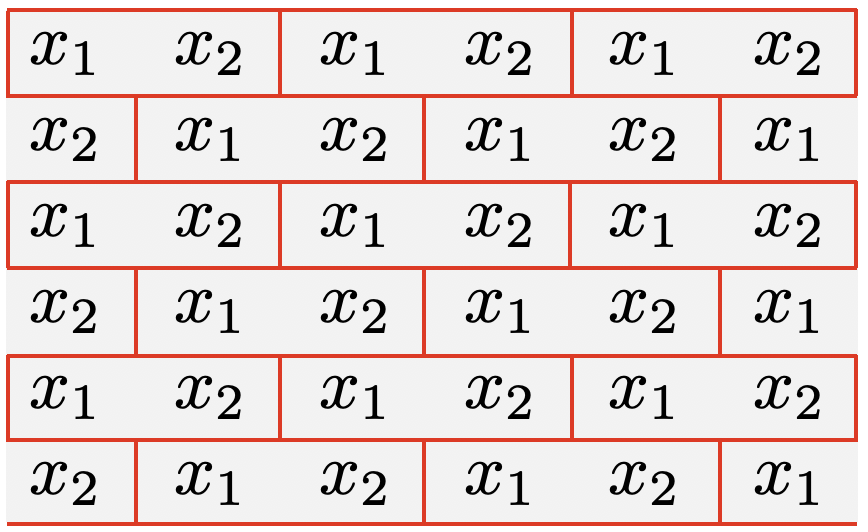
\includegraphics[width=1.0\textwidth]{HL2by1RelativePeriodicBlock}\\(a)
            \end{center}\end{minipage}
            \hskip 4ex
            \begin{minipage}[c]{0.46\textwidth}\begin{center}
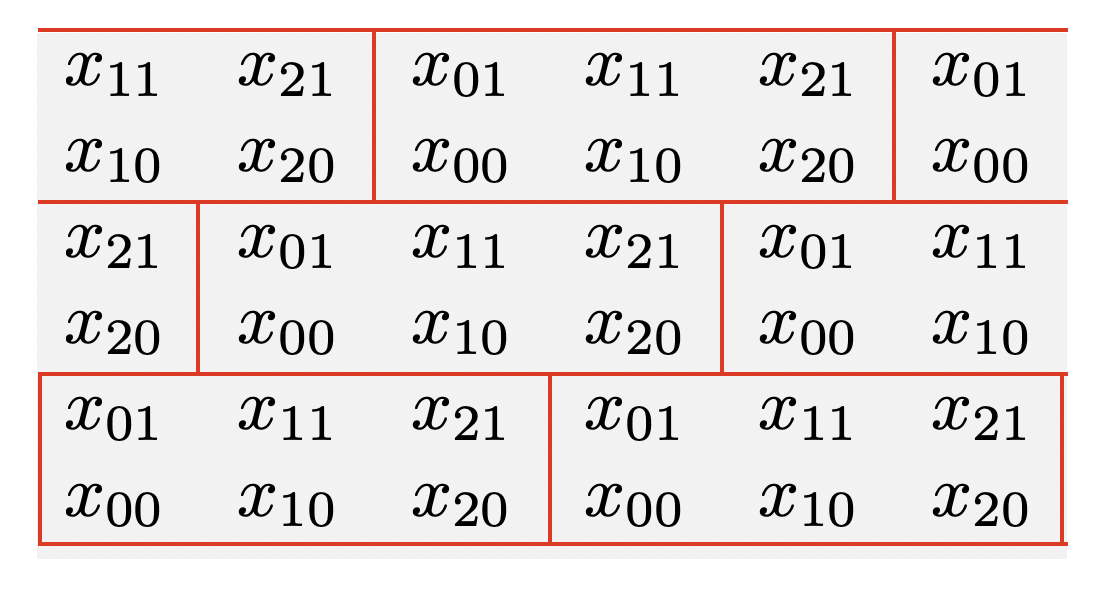
\includegraphics[width=1.0\textwidth]{HL2by3RelativePeriodicBlock}\\(b)
            \end{center}\end{minipage}
\end{center}
  \caption{\label{fig:2x1rpo}
Examples of $\LTS{}{}{}$ \twots\
together with their \spt\ Bravais lattice tilings \refeq{2DBravaisLattice}.
(a)
$\BravCell{2}{1}{1}$, basis vectors
$\mathbf{a}_1=\{2,0\}$ and $\mathbf{a}_2=\{1,1\}$;
(b)
$\BravCell{3}{2}{1}$, basis vectors
$\mathbf{a}_1=(3,0)$ and $\mathbf{a}_2=(1,2)$.
Rectangles enclose the Bravais cell and its Bravais lattice
translations.
}
\end{figure}
%%%%%%%%%%%%%%%%%%%%%%%%%%%%%%%%%%%%%%%%%%%%%%%%%%%%%%%%%%%%%%%




%\subsection{Admissible prime \twots}
%\label{s:prime2tAdmiss}
    \PC{2020-06-09}{explain \reftab{tab:LxTs}}

\begin{description}



	\HLpost{2020-06-09}{
\refFigs{fig:SpecialBravaisLatt}{fig:3x2rpo} are the plots of the
periodic \brick s by color. The three figures in
\reffig{fig:SpecialBravaisLatt} are the \brick s with periodicity
$\BravCell{1}{3}{0}$, $\BravCell{3}{1}{0}$ and $\BravCell{3}{1}{1}$,
which can show the periodicity of the space-\eqva, time-\eqva\ and
time-\reqva. \refFig{fig:3x2rpo} is the color coding of the periodic
blocks with periodicity $\BravCell{2}{1}{1}$, $\BravCell{3}{2}{1}$ and
$\BravCell{3}{2}{0}$.
	}

%%%%%%%%%%%%%%%%%%%%%%%%%%%%%%%%%%%%%%%%%%%%%%%%%%%%%%%%%%%%%
% HL 2020-06-09 siminos/figSrc/han/Mathematica/ColorBlock.nb
\begin{figure}\begin{center}
            \begin{minipage}[c]{0.25\textwidth}\begin{center}
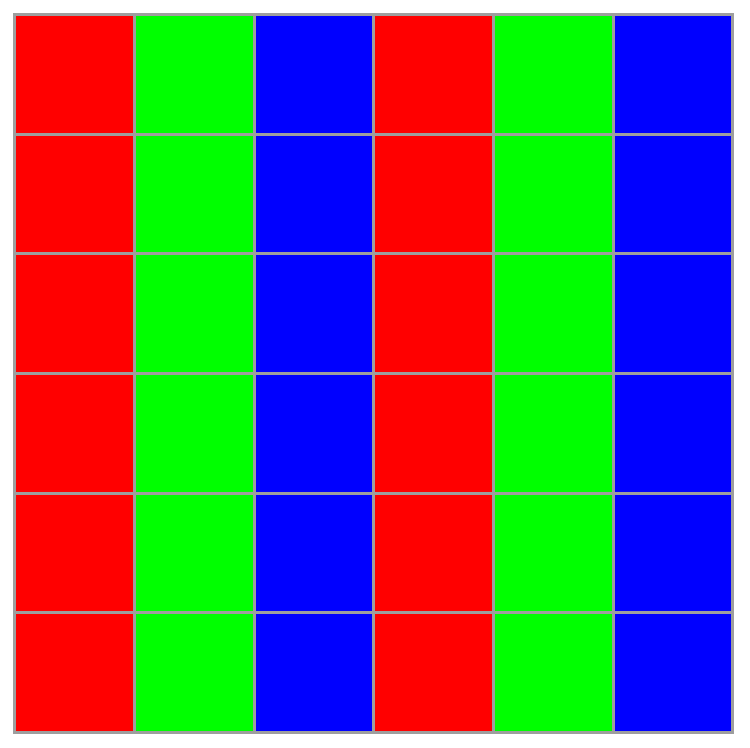
\includegraphics[width=1.0\textwidth]{HL310Block}\\(a)
            \end{center}\end{minipage}
            \hskip 4ex
            \begin{minipage}[c]{0.25\textwidth}\begin{center}
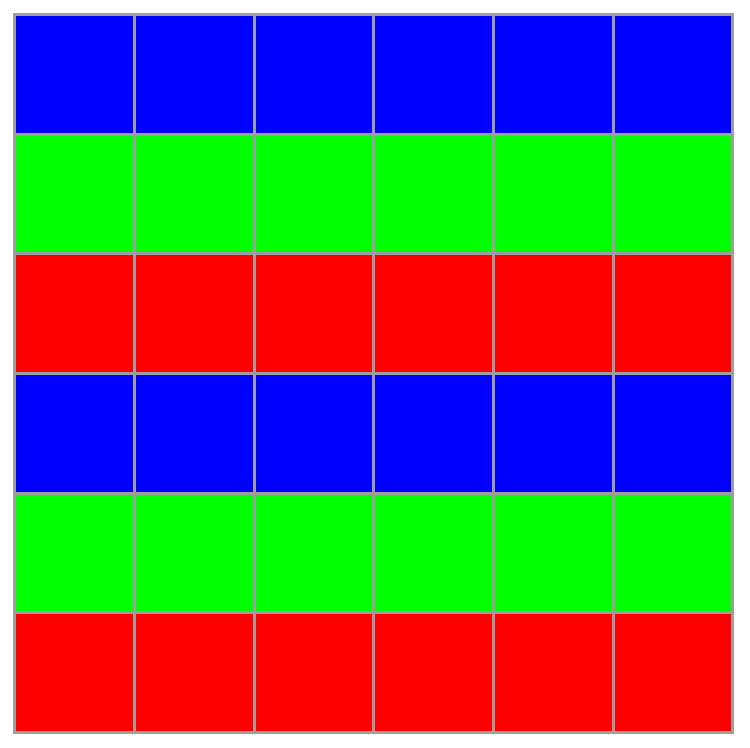
\includegraphics[width=1.0\textwidth]{HL130Block}\\(b)
            \end{center}\end{minipage}
            \hskip 4ex
            \begin{minipage}[c]{0.25\textwidth}\begin{center}
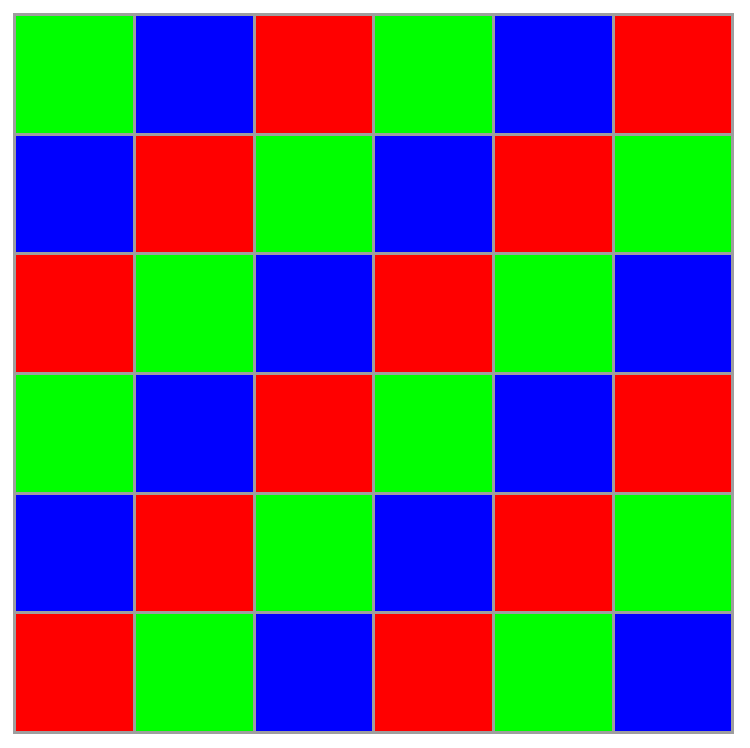
\includegraphics[width=1.0\textwidth]{HL311Block}\\(c)
            \end{center}\end{minipage}
\end{center}
  \caption{\label{fig:SpecialBravaisLatt}
Examples of $\LTS{}{}{}$ periodic \brick s
together with their \spt\ Bravais lattice tilings \refeq{2DBravaisLattice}.
(a)
$\BravCell{3}{1}{0}$, basis vectors
$\mathbf{a}_1=\{3,0\}$ and $\mathbf{a}_2=\{0,1\}$;
(b)
$\BravCell{1}{3}{0}$, basis vectors
$\mathbf{a}_1=\{1,0\}$ and $\mathbf{a}_2=\{0,3\}$;
(c)
$\BravCell{3}{1}{1}$, basis vectors
$\mathbf{a}_1=\{3,0\}$ and $\mathbf{a}_2=\{1,1\}$;
}
\end{figure}
%%%%%%%%%%%%%%%%%%%%%%%%%%%%%%%%%%%%%%%%%%%%%%%%%%%%%%%%%%%%%%%

%%%%%%%%%%%%%%%%%%%%%%%%%%%%%%%%%%%%%%%%%%%%%%%%%%%%%%%%%%%%%
% HL 2020-06-09 siminos/figSrc/han/Mathematica/ColorBlock.nb
\begin{figure}\begin{center}
            \begin{minipage}[c]{0.25\textwidth}\begin{center}
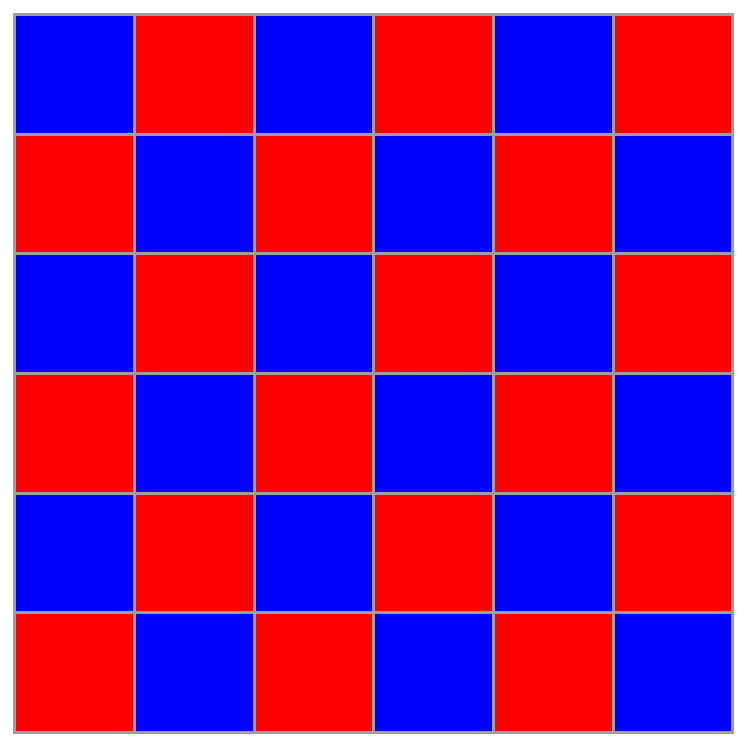
\includegraphics[width=1.0\textwidth]{HL211Block}\\(a)
            \end{center}\end{minipage}
            \hskip 4ex
            \begin{minipage}[c]{0.25\textwidth}\begin{center}
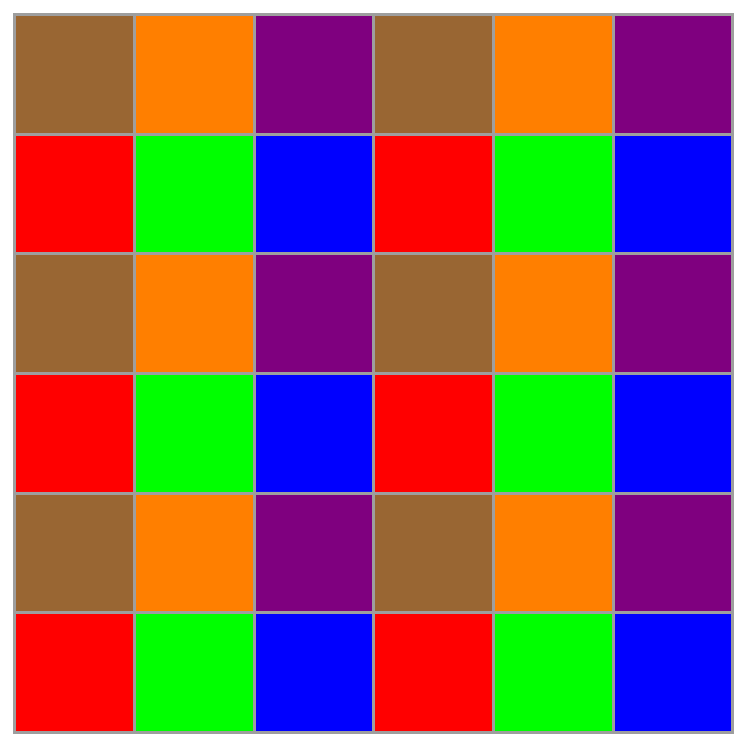
\includegraphics[width=1.0\textwidth]{HL320Block}\\(b)
            \end{center}\end{minipage}
            \hskip 4ex
            \begin{minipage}[c]{0.25\textwidth}\begin{center}
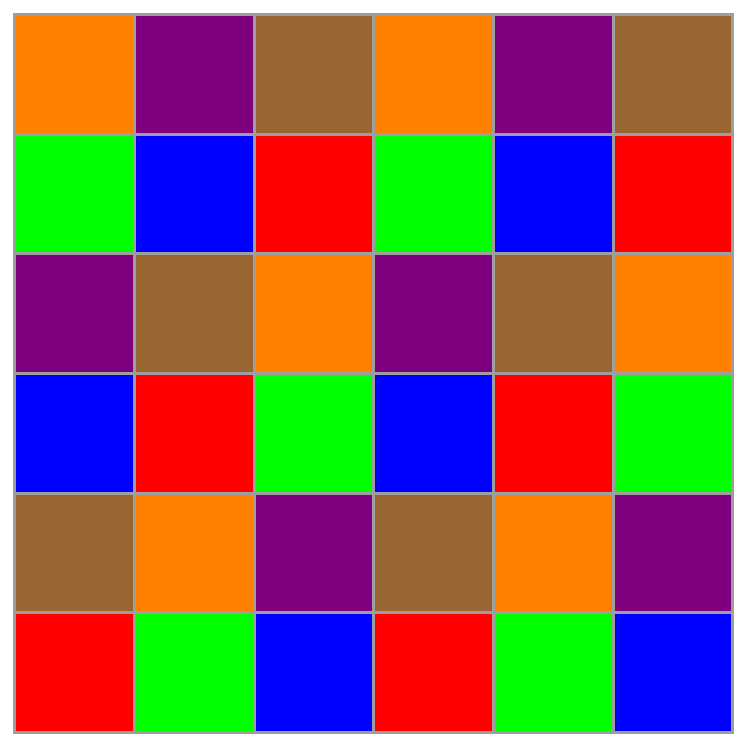
\includegraphics[width=1.0\textwidth]{HL321Block}\\(c)
            \end{center}\end{minipage}
\end{center}
  \caption{\label{fig:3x2rpo}
Examples of $\LTS{}{}{}$ periodic \brick s
together with their \spt\ Bravais lattice tilings \refeq{2DBravaisLattice}.
(a)
$\BravCell{2}{1}{1}$, basis vectors
$\mathbf{a}_1=\{2,0\}$ and $\mathbf{a}_2=\{1,1\}$;
(b)
$\BravCell{3}{2}{0}$, basis vectors
$\mathbf{a}_1=\{3,0\}$ and $\mathbf{a}_2=\{0,2\}$;
(c)
$\BravCell{3}{2}{1}$, basis vectors
$\mathbf{a}_1=\{3,0\}$ and $\mathbf{a}_2=\{1,2\}$;
}
\end{figure}
%%%%%%%%%%%%%%%%%%%%%%%%%%%%%%%%%%%%%%%%%%%%%%%%%%%%%%%%%%%%%%%



    \PCpost{2019-11-23}{
We always reduce relative-shift symmetries, so I am not happy about the
$\BravCell{2}{1}{1}$ relative-periodic {\brick} \refeq{eq:block2x1rp} being
counted as the $\BravCell{2}{2}{0}$ \twot. We'll have to revisit symmetry
reduction...
    }


	\HLpost{2020-03-17}{
\emph{PrimeTiles.nb} generates all prime tiles that can tile a
larger tile. It gives
some not obvious results. For example, let the large tile be
$\BravCell{3}{2}{1}$, and consider the full-shift 9-symbol
$\BravCell{3}{2}{1}$ \brick s. The number $\BravCell{3}{2}{0}$ \brick s is
given by \refeq{catlattN3x2}. The program shows that the
$\BravCell{3}{2}{0}$ tile can only be tiled by $\BravCell{1}{1}{0}$,
$\BravCell{1}{2}{0}$ and $\BravCell{3}{1}{0}$ tiles. So we get the result in
\refeq{catlattN3x2}:
\[
N_{\BravCell{3}{2}{0}} = 9^{3\times2} =
88440\,\BravCell{3}{2}{0}+240\,\BravCell{3}{1}{0}
  +36\,\BravCell{1}{2}{0}+9\,\BravCell{1}{1}{0}
\,.
\]
For the full-shift the number of periodic \brick s is given
by the area of the larger tile, and number of $\BravCell{3}{2}{\slant{}}$ \brick
s is the same for all $S$. But now
$\BravCell{3}{1}{0}$ tile cannot tile the $\BravCell{3}{2}{1}$ tile.
Instead, the $\BravCell{3}{2}{1}$ can be tiled by
$\BravCell{1}{1}{0}$, $\BravCell{3}{1}{2}$  and $\BravCell{1}{2}{0}$ tiles,
 \[
N_{\BravCell{3}{2}{1}} = 9^{3\times2} =
88440\,\BravCell{3}{2}{1}+ 240\,\BravCell{3}{1}{2}+36\,\BravCell{1}{2}{0}
   +9\,\BravCell{1}{1}{0}
\,.
\]
\emph{A priori} is not obvious that $\BravCell{3}{1}{2}$ tile can tile a
$\BravCell{3}{2}{1}$ tile. But if you stack $\BravCell{3}{1}{2}$ tile in the
shifted temporal direction by 2 then the left edge of the tile is shifted
by 4 in the spatial direction. With the spatial period being 3, shifted
by 4 in the spatial direction is same as shifted by 1. So the \bcs\ of
$\BravCell{3}{2}{1}$ tile are satisfied by the $\BravCell{3}{1}{2}$ tiles.
    }


\end{description}


%%%%%%%%%%%%%%%%%%%%%%%%%%%%%%%%%%%%%%%%%%%%%%%%%%%%%%%%%%%%%%%%%%%%%%%
%\printbibliography[heading=subbibintoc,title={References}]

    \ifboyscout\clearpage\fi
% siminos/kittens/Hill.tex      pdflatex CL18
% $Author: predrag $ $Date: 2020-09-21 23:51:15 -0500 (Mon, 21 Sep 2020) $

\section{{\HillDet}:
            stability of an orbit vs. its time-evolution stability}
\label{s:Hill}

The $d=2$ lattice \catlatt\ equations can be recast in a matrix form, by
rewriting the defining equations in terms of \emph{block
matrices}\rf{Dorr70,BuGoNi70,ChenM87,HuRyCo98}, constructed by the
\HREF{https://en.wikipedia.org/wiki/Kronecker_product} {Kronecker
product} $\mathbf{A}\otimes\mathbf{B}$, an operation
(introduced by Zehfuss in 1858) that replaces the $a_{ij}$
element of an [$n\times{n}$] matrix $\mathbf{A}$ by [$m\times{m}$]
matrix block $a_{ij}\mathbf{B}$, resulting in an [$mn\times mn$] block
matrix\rf{ArWeHa13,wikiKronProd}
\beq
\mathbf{A}\otimes\mathbf{B} =
\left[\begin{array}{ccc} %\begin{bmatrix}
  a_{11} \mathbf{B} & \cdots & a_{1n}\mathbf{B} \\
             \vdots & \ddots &           \vdots \\
  a_{n1} \mathbf{B} & \cdots & a_{nn} \mathbf{B}
\end{array}\right] %\end{bmatrix}
\,.
\ee{KronProd}
Consider $\mathbf{A}$, $\mathbf{A'}$ square matrices of size
[$n\times{n}$], and $\mathbf{B}$, $\mathbf{B'}$ square matrices of size
[$m\times{m}$].
The matrix product of two block matrices is a block
matrix\rf{ArWeHa13,wikiBlockMat},
\beq
(\mathbf{A}\otimes\mathbf{B})\,(\mathbf{A'}\otimes\mathbf{B'})
%= (\mathbf{A}\mathbf{A'})\otimes(\mathbf{B}\mathbf{D})
%  {\displaystyle (\mathbf {A} \otimes \mathbf {B} )(\mathbf {C} \otimes \mathbf {D} )
  =(\mathbf{AA'})\otimes (\mathbf{BB'})
  \,.
\ee{mixedProd}
The trace and the determinant of a block matrix are given by
\bea
\tr(\mathbf {A} \otimes \mathbf {B})
    &=& \tr\mathbf{A}\,\tr\mathbf{B}
    \continue
\det\left(\mathbf{A} \otimes \mathbf{B}\right)
    &=& \det\left(\mathbf{A}^{m}\right) \det\left(\mathbf{B}^{n}\right)
\,.
\label{wikiKron2}
\eea
The two [$mn\times mn$] block matrices $\mathbf{A}\otimes\mathbf{B}$ and
$\mathbf{B}\otimes\mathbf{A}$ are equivalent by a similarity
transformation
\beq
\mathbf {B} \otimes \mathbf {A}
=\transp{\mathbf {P}} \,(\mathbf {A} \otimes \mathbf {B} )\,\mathbf {P}
\,,
\ee{wikiKron3}
where $\mathbf{P}$ is permutation matrix. As $\det{\mathbf{P}}=1$,
the block matrix determinant
$\det\left(\mathbf{A}\otimes\mathbf{B}\right)
=
\det\left(\mathbf{B}\otimes\mathbf{A}\right)$
is independent of the order in which blocks are constructed.

Consider a rectangular $d=2$ lattice
$\BravCell{\speriod{}}{\period{}}{0}$ Bravais cell. The \jacobianOrb\
\refeq{catLatt} written as a
$[\speriod{}\period{}\times\speriod{}\period{}]$ Kronecker product block
matrix is
\beq
\jMorb
=
\unit_{1} \otimes \left(\hopMat_{2}+\hopMat_{2}^{-1}\right)
-
2 {s}\,\unit_1\otimes\unit_{2}
+
\left(\hopMat_{1}+\hopMat_{1}^{-1}\right) \otimes \unit_{2}
\,,
\ee{catalattLxT}
where the \refeq{KronProd} matrix $\mathbf{A}$ and identity
$\unit_1$ matrix are `spatial' [$\speriod{}\!\times\!\speriod{}$]
matrices, with blocks $\mathbf{B}$ and identity $\unit_2$ `temporal'
[$\period{}\!\times\!\period{}$] matrix blocks. Indices `1', `2'
referring to `spatial', `temporal' lattice directions, respectively.

Our task is to compute the {\HillDet} $|\det \jMorb|$. We first show how
to do that directly, by computing the volume of the {\fundPip}.

\subsection{{\HillDet}: fundamental parallelepiped evaluation}
\label{s:catLattRel3x2}
% 2020-02-16 Predrag computed  using siminos/mathematica/Tensors.nb
As a concrete example
consider the Bravais lattice \refeq{2DBravaisLattice} with basis
vectors $\mathbf{a}_1=(3,0)$ and $\mathbf{a}_2=(0,2)$. A \twot\ over this
Bravais cell has 6 field values, one for each lattice site $z=(n,\zeit)$
on a $\BravCell{3}{2}{0}$ rectangle:
\[
 \left[\begin{array}{ccc}
 \ssp_{01} & \ssp_{11} & \ssp_{21} \\
 \ssp_{00} & \ssp_{10} & \ssp_{20}
 \end{array}\right]
\,.
\]
Stack up the columns of this lattice state and the corresponding sources
into 6\dmn\ vectors,
\beq
\Xx_{\BravCell{3}{2}{0}} =
\left(\begin{array}{c}
 \ssp_{01} \\
 \ssp_{00} \\
  \hline
 \ssp_{11} \\
 \ssp_{10} \\
  \hline
 \ssp_{21} \\
 \ssp_{20} \\
      \end{array}\right)
\,,\qquad
\Mm_{\BravCell{3}{2}{0}} =
\left(\begin{array}{c}
 \Ssym{01} \\
 \Ssym{00} \\
  \hline
 \Ssym{11} \\
 \Ssym{10} \\
  \hline
 \Ssym{21} \\
 \Ssym{20} \\
        \end{array}\right)
\,.
\ee{3times2blockVect}
The corresponding {\jacobianOrb} \refeq{catlattFix}
%\([\BravCell{3}{2}{}\times \BravCell{3}{2}{}]\)
%4-index matrix $\jMorb_{zz'}$.
is the  block-matrix
\refeq{catalattLxT},
a block circulant matrix
with circulant blocks\rf{ChenM87},
\beq
\jMorb_{\BravCell{3}{2}{0}} =
\left(
\begin{array}{cc|cc|cc}
 -2 s & 2 & 1 & 0 & 1 & 0  \\
 2 & -2 s & 0 & 1 & 0 & 1  \\
  \hline
 1 & 0 & -2 s & 2 & 1 & 0  \\
 0 & 1 & 2 & -2 s & 0 & 1  \\
  \hline
 1 & 0 & 1 & 0 & -2 s & 2  \\
 0 & 1 & 0 & 1 & 2 & -2 s
\end{array}
\right)
\,.
\ee{3times2blockMat}
of $[\speriod{}\!\times\!\speriod{}]$ block form, $\speriod{}=3$,
with $[\period{}\!\times\!\period{}]$ blocks, $\period{}=2$.

The {\fundPip} generated by the action of {\jacobianOrb}
$\jMorb_{\BravCell{3}{2}{0}}$ is spanned by $\speriod{}\period{}=6$ basis
vectors, the columns \refeq{lattJac} of the {\jacobianOrb}
\refeq{3times2blockMat}:
\beq
\jMorb_{\BravCell{3}{2}{0}} =
\left(
\begin{array}{c|c|c|c|c|c}
 -2 s & 2 & 1 & 0 & 1 & 0  \\
 2 & -2 s & 0 & 1 & 0 & 1  \\
 1 & 0 & -2 s & 2 & 1 & 0  \\
 0 & 1 & 2 & -2 s & 0 & 1  \\
 1 & 0 & 1 & 0 & -2 s & 2  \\
 0 & 1 & 0 & 1 & 2 & -2 s
\end{array}
\right)
\,.
\ee{3times2basisVecs}
The `fundamental fact' \refeq{detBern0} now yields the {\HillDet}
as the number of
doubly-periodic lattice states,
\beq
N_{\BravCell{3}{2}{0}} = |\Det\jMorb_{\BravCell{3}{2}{0}}|
                   = 4({s}-2)s(2{s}-1)^2 (2{s}+3)^2
\,.
\ee{N3times2}

\subsection{{\HillDet}: time-evolution evaluation}
\label{s:HillHam}

In practice, one often
computes the {\HillDet} using a  Hamiltonian, or `transfer matrix'
formulation. An example is the \templatt\ 3-term recurrence
\refeq{catMapNewt} in the \PV\rf{PerViv} `two-configuration' cat map
representation \refeq{eq:StateSpCatMap}
\beq
 \hat{\mathbf{\ssp}}_{\zeit+1} =
      {\hat{\mathbf{\jMps}}_1}\,\hat{\mathbf{\ssp}}_\zeit - \hat{\mathsf{\Ssym{}}}_\zeit
\,,
\ee{PV2config}
with the one-time step temporal evolution [$2\!\times\!2$] {\jacobian}
matrix ${\hat{\mathbf{\jMps}}_1}$ generating a time orbit by acting on the
2\dmn\ `phase space' of successive configuration points
\beq
 {\hat{\mathbf{\jMps}}_1}
=
 \left[\begin{array}{cc}
 0 & 1 \\
 -1 & s
 \end{array} \right]
\,,\qquad
\hat{\mathbf{\ssp}}_\zeit
=
\left[\begin{array}{c}
 \ssp_{\zeit-1}\\
 \ssp_{\zeit}
\end{array}\right]
\,,\qquad
\hat{\mathsf{\Ssym{}}}_\zeit
=
\left[\begin{array}{c}
 0           \\
 \Ssym{\zeit}
\end{array}\right]
\,,
\ee{PV2configJ}
Similarly, for the $d=2$ \catlatt\ lattice at hand, one can
recast the 5-term recurrence \refeq{CatMap2d}
\bea
\ssp_{n\zeit}
&=& ~~\ssp_{n\zeit}
%(- \ssp_{n+1,\zeit-1} + 2{s} \, \ssp_{n,\zeit-1} - \ssp_{n-1,\zeit-1})
%- \Ssym{n,\zeit-1}
%- \ssp_{n,\zeit-2}
    \continue
\ssp_{n,\zeit+1}
&=&  - \ssp_{n,\zeit-1}
 +(- \ssp_{n-1,\zeit} + 2{s} \, \ssp_{n\zeit} - \ssp_{n+1,\zeit})
- \Ssym{n\zeit}
%\,,
\label{CatMap2dHill}
\eea
in the `two-configuration' matrix form \refeq{PV2config} by picking the
vertical direction (indexed `2') as the `time', with temporal 1-time step {\jacobian}
[$2\speriod{}\!\times\!2\speriod{}$] block matrix
% ${\hat{\mathbf{\jMps}}_1}$
\beq
{\hat{\mathbf{\jMps}}_1}  =
 \left[\begin{array}{c|c}
{\bf 0} & \unit_1\\ \hline
-\unit_1 & {-\mathbf{\jMorb}_1}
 \end{array} \right]
\,,
\ee{PV2catlattJ}
(known as a transfer matrix in statistical
mechanics\rf{Onsager44,MonMun94}) generating a `time'orbit by acting on a
$2\speriod{}$\dmn\ `phase space'  lattice strip
$\hat{\mathbf{\ssp}}_\zeit$ along the `spatial' direction  (indexed `1'),
\[  %\beq
\hat{\mathbf{\ssp}}_\zeit
=
\left[\begin{array}{c}
 {\mathbf{\ssp}}_{\zeit-1}\\ \hline
 {\mathbf{\ssp}}_\zeit
 \end{array}\right]
,\quad
\hat{\mathsf{\Ssym{}}}_\zeit
=
    \left[\begin{array}{c}
    \mathbf{0}\\ \hline
 \mathbf{\Ssym{}}_{\zeit}
 \end{array}\right]
,\qquad
\mathbf{\ssp}_\zeit
=
\left[\begin{array}{c}
 \ssp_{1\zeit}\\   \vdots\\ \ssp_{\speriod{}\zeit}
 \end{array}\right]
,\quad
\mathsf{\Ssym{}}_\zeit
=
    \left[\begin{array}{c}
 \Ssym{1\zeit}\\ \vdots\\ \Ssym{\speriod{}\zeit}
 \end{array}\right]
,
\] %\ee{PV2catlattJ1}
where the hat $\hat{~}$~ indicates a $2\speriod{}$\dmn\
`two-configuration' state, and $\mathbf{\jMorb}_1$ is the spatial
$[\speriod{}\!\times\!\speriod{}]$ {\jacobianOrb} of
$d=1$ \templatt\ form \refeq{tempCatFix},
\beq
\mathbf{\jMorb}_1
        =
\hopMat_{1}^{-1} - 2s \unit_1 + \hopMat_{1}
\label{Hessian_Hill}
\eeq
The `two-configuration' coupled cat maps system \refeq{PV2config} is a
generalization of the Bernoulli map time evolution formulation
\refeq{tempBern} to a high-dimensional spatially-coupled lattice. Just as
in the {temporal Bernoulli} condition \refeq{tempFixPoint}, the first
order in time difference equation \refeq{PV2config} can be viewed as a
lattice state fixed point condition \refeq{tempFixPoint}, a zero of the
function
\( %beq
F[\hat{\Xx}] = \hat{\mathbf{\jMorb}}\hat{\Xx}+\hat{\Mm} = 0
\,,
\) %\ee{tempPV2Point}
with the entire periodic \emph{lattice state} $\hat{\Xx}_{\Mm}$ treated as a
single fixed \emph{point} in the
$2\speriod{}\period{}$\dmn\ \statesp\ unit hyper-cube, and the
$[2\speriod{}\period{}\times2\speriod{}\period{}]$  block matrix \jacobianOrb\
given either by
\beq
\hat{\mathbf{\jMorb}} =
    \hat{\unit} - {\hat{\mathbf{\jMps}}_1}\otimes\hopMat_2^{-1}
\,,
\ee{tempPV2conf12}
or by
\beq
\hat{\mathbf{\jMorb}}' =
    \hat{\unit} -\hopMat_2^{-1} \otimes {\hat{\mathbf{\jMps}}_1}
\,.
\ee{tempPV2conf21}
Here the unity $\hat{\unit}=\hat{\unit}_1\otimes\unit_{2}$ is a
[$2\speriod{}\period{}\!\times\!2\speriod{}\period{}$] block matrix, and
the time-evolution \jacobianM\ ${\hat{\mathbf{\jMps}}_1}$
\refeq{PV2catlattJ} is a [$2\speriod{}\!\times\!2\speriod{}$] matrix.

The order in which the block matrix blocks are composed does not matter,
yielding the same the {\HillDet} $\det\hat{\mathbf{\jMorb}} =
\det\hat{\mathbf{\jMorb}}'$ by \refeq{wikiKron3}.
However, written out explicitly, the two \jacobianOrbs\
\refeq{eq:orbitJPVJxS} and \refeq{eq:orbitJPVtempJ} are of a very
different form.

For example, for the $\BravCell{\speriod{}}{\period{}}{0}$  rectangular
Bravais cell, the \catlatt\ \jacobianOrb\ \refeq{tempPV2conf12} involves the
[$\period{}\!\times\!\period{}$] time {\shiftOp} block matrix $\hopMat_2$
\refeq{hopMatrix} with the one-time-step [$2\speriod{}\!\times\!2\speriod{}$]
time-evolution \jacobianM\ ${\hat{\mathbf{\jMps}}_1}$ \refeq{PV2catlattJ}
\bea
\hat{\mathbf{\jMorb}}
    &=&
\left[\begin{array}{c|c}
 \unit_{1}\otimes\unit_{2}   & -\unit_1\otimes\hopMat_2^{-1}             \\ \hline
 \unit_1\otimes\hopMat_2^{-1}& \unit_{1}\otimes\unit_{2} +\mathbf{\jMorb}_1\otimes\hopMat_2^{-1}
\end{array}\right]
\,,
\label{eq:orbitJPVJxS}
\eea
and for \catlatt\ \refeq{CatMap2dHill} this is a time-periodic
[$\period{}\times\period{}$]  {\shiftOp} block matrix $\hopMat_2$
\refeq{hopMatrix}, each block now a space-periodic
[$2\speriod{}\!\times\!2\speriod{}$] matrix ${\hat{\mathbf{\jMps}}_1}$
\refeq{PV2catlattJ}.

If a block matrix is composed of four blocks,
\HREF{https://en.wikipedia.org/wiki/Block_matrix\#Block_matrix_inversion}
{its determinant} can be evaluated using Schur's 1917
formula\rf{Schur1917,wikiBlockMat}
%From \refeq{det2x2blockMat*** we have
\beq
\det\left[\begin{array}{c|c}
\mathbf{A} & \mathbf{B} \\ \hline
\mathbf{C} & \mathbf{D}
\end{array}\right]
=
\det(\mathbf{A})\,\det(\mathbf{D}-\mathbf{C}\mathbf{A}^{-1}\mathbf{B})
\,.
\ee{det2x2blockMat}
so, noting \refeq{mixedProd}, \refeq{catalattLxT} and
\refeq{Hessian_Hill}, we find that
\bea
\det\hat{\mathbf{\jMorb}}
    &=&
\det\left[\begin{array}{c|c}
 \unit_{1}\otimes\unit_{2}   & -\unit_1\otimes\hopMat_2^{-1}             \\ \hline
 \unit_1\otimes\hopMat_2^{-1}& \unit_{1}\otimes\unit_{2} +\mathbf{\jMorb}_1\otimes\hopMat_2^{-1}
\end{array}\right]
     \continue
     &=&
% \det(\unit_1)\,
\det\left[
       \unit_{1}\otimes\unit_{2} + \mathbf{\jMorb}_1\otimes\hopMat_2^{-1}
     + (\unit_1\otimes\hopMat_2^{-1})(\unit_{1}\otimes\unit_{2})(\unit_1\otimes\hopMat_2^{-1})
    \right]
     \continue
     &=&
\det\left[
       \unit_{1}\otimes\unit_{2} + \mathbf{\jMorb}_1\otimes\hopMat_2^{-1}
     +  \unit_1\otimes\hopMat_2^{-2}
    \right]
     \continue
     &=&
\det(\unit_1\otimes\hopMat_2^{-1})\,
\det\left[
       \unit_1\otimes\hopMat_2^{-1}
        +(\hopMat_{1}^{-1} - 2s \unit_1 + \hopMat_{1})\otimes\unit_2
     +  \unit_1\otimes\hopMat_2
    \right]
     \continue
     &=&
\det \jMorb
\,,
\label{det2x2blockMat2LH}
\eea
where we have used
$\det\unit_{1}=\det\unit_{2}=\det\hopMat_{1}=\det\hopMat_{2}=1$.

This proves that $\det\hat{\mathbf{\jMorb}}$ of the
`Hamiltonian' or `two-configuration'
$[2\speriod{}\period{}\times2\speriod{}\period{}]$ `phase space'
\jacobianOrb\ $\hat{\mathbf{\jMorb}}$ defined by \refeq{eq:orbitJPVJxS}
equals the `Lagrangian' {\HillDet} of the
$[\speriod{}\period{}\times\speriod{}\period{}]$ \jacobianOrb\
$\mathbf{\jMorb}$.

\subsection{Hill's formula}
\label{s:HillForm}

Consider next \refeq{tempPV2conf21}, the equivalent way of forming of the
block matrix for the $\BravCell{\speriod{}}{\period{}}{0}$  rectangular
Bravais cell, with temporal period taken for definitiveness
$\period{}=4$. The \catlatt\ \jacobianOrb\ \refeq{tempPV2conf21} is now
constructed as the [$4\times4$] time {\shiftOp} block matrix $\hopMat_2$
\refeq{hopMatrix}, with the one-time-step
[$2\speriod{}\!\times\!2\speriod{}$] time-evolution \jacobianM\
${\hat{\mathbf{\jMps}}_1}$ \refeq{PV2catlattJ} and unit matrix
$\hat{\unit}_1$ as blocks
\beq
\hat{\mathbf{\jMorb}}'
 =
\unit_2\otimes\hat{\unit}_{1} -\hopMat_2^{-1} \otimes {\hat{\mathbf{\jMps}}_1}
 =
\left[\begin{array}{c|c|c|c}
 \hat{\unit}_1    &  {\bf 0}   & {\bf 0}    &-{\hat{\mathbf{\jMps}}_1} \\ \hline
-{\hat{\mathbf{\jMps}}_1} &  \hat{\unit}_1   & {\bf 0}    & {\bf 0}    \\ \hline
 {\bf 0}    &-{\hat{\mathbf{\jMps}}_1} & \hat{\unit}_1    & {\bf 0}    \\ \hline
 {\bf 0}    &  {\bf 0}   &-{\hat{\mathbf{\jMps}}_1} & \hat{\unit}_1
\end{array}\right]
\,.
\label{eq:orbitJPVtempJ}
\eeq
The {\HillDet} $\det\hat{\mathbf{\jMorb}}'$ evaluation follows
essentially the same path as the Bernoulli {\HillDet} evaluation of
\refsect{s:bernCount}, generalized to block matrices. From the
block-matrix multiplication rule \refeq{mixedProd} and the determinant
rule \refeq{wikiKron2} it follows that
\beq
(\hopMat_2^{-1}\otimes{\hat{\mathbf{\jMps}}_1})
(\hopMat_2^{-1}\otimes{\hat{\mathbf{\jMps}}_1})
=
\hopMat_2^{-2}\otimes{\hat{\mathbf{\jMps}}_1}^2
\,,\quad\mbox{ so }
(\hopMat_2^{-1} \otimes {\hat{\mathbf{\jMps}}_1})^k =
\hopMat_2^{-k} \otimes {\hat{\mathbf{\jMps}}_1}^k
\,,
\ee{shiftPower}
and
\beq
\det(\hopMat_2^{-1}\otimes{{\hat{\mathbf{\jMps}}_1}})
=
(\det\hopMat_2)^{-\speriod{}}
(\det{\hat{\mathbf{\jMps}}_1})^\period{}
=
\det\hat{\mathbf{\jMps}}_p
\,,\qquad
\hat{\mathbf{\jMps}}_p = {\hat{\mathbf{\jMps}}_1}^\period{}
\,,
\ee{detShiftxJ}
where $\hat{\mathbf{\jMps}}_p$ is the {\jacobianM} of a
temporal periodic orbit $p$.
Expand
\(
 \ln\det\hat{\mathbf{\jMorb}}'
   =
 \tr\ln\hat{\mathbf{\jMorb}}'
\)
as a series using \refeq{wikiKron2} and \refeq{shiftPower},
\beq
\tr\ln\hat{\mathbf{\jMorb}}' =
\tr\ln(\unit-\hopMat_2^{-1} \otimes {{\hat{\mathbf{\jMps}}_1}})
  =
-\sum_{k=1}^\infty\frac{1}{k}{\tr(\hopMat_2^{-k})}\,\tr{{\hat{\mathbf{\jMps}}_1}}^{k}
\,,
\ee{LnDet=TrLn_Hill}
and use
$\tr \hopMat_2^k=\period{}$
if $k$ is a multiple of $\period{}$,
0 otherwise
(follows from $\hopMat_2^\period{}=\unit$):
\[
\ln\det(\unit-\hopMat_2^{-1} \otimes {{\hat{\mathbf{\jMps}}_1}})
  =
-\sum_{r=1}^\infty\frac{1}{r}\tr\hat{\mathbf{\jMps}}_p^{r}
  =
\ln\det(\hat{\unit}_{1}-\hat{\mathbf{\jMps}}_p)
\,.
\]
So for the {\catlatt} the {\jacobianOrb}  and the temporal evolution
\refeq{PV2config} stability ${{\hat{\mathbf{\jMps}}_{p}}}$ are related by
the remarkable (discrete time) Hill's formula\rf{MacMei83,BolTre10}
\beq
|\det\jMorb|
  =
|\det(\hat{\unit}_{1}-\hat{\mathbf{\jMps}}_p)|
\,.
\ee{HillDet}
which expresses the  {\HillDet} of the arbitrarily large \jacobianOrb\
$\jMorb$  in terms of a determinant of a small
[$2\speriod{}\!\times\!2\speriod{}$] time-evolution \jacobianM\
$\hat{\mathbf{\jMps}}_p$.


\bigskip

Two remarks.
First, the reformulation of the \catlatt\ 5-term recurrence
\refeq{CatMap2dHill} as the `two-configuration' form \refeq{PV2config} is
a passage from the Lagrangian to the Hamiltonian formulation, also known
as `transfer matrix' formulation of lattice field
theories\rf{MonMun94,MunWal00} and Ising
models\rf{Onsager44,Kastening02}. We chose to prove it here using only
elementary linear algebra, not only because the Lagrangian
formalism\rf{BolTre10} is not needed for the problem at hand, but because
it actually obscures the generality of Hill's formula, which works
equally well for dissipative systems (see Bernoulli Hill's formula
\refeq{noPerPts}), with no Lagrangian formulation.

Second,
for Hamiltonian evolution \refeq{catMap}, the $[2\!\times\!2]$
\jacobianM\ $\jMps^\period{}$ (the monodromy matrix of a \po) describes
the growth of an initial state perturbation in $\period{}$ steps. For the
corresponding Lagrangian system with action $\action$,
% (see \refsect{s:catLagrForm}),
the first variation of
the action $\delta\action=0$ yields the \templatt\ condition
\refeq{catTempLatt}, while the second variation, the
$[\period{}\!\times\!\period{}]$ {\jacobianOrb} \refeq{tempCatFix},
describes the stability of the \emph{entire} given \po. In this,
classical mechanics context, Bolotin and Treschev\rf{BolTre10} refer to
$\jMorb$ as the `Hessian operator', but, as it is clear from our
Bernoulli discussion of \refsect{s:JacobianOrb}, and applications to \KS\
and Navier-Stokes systems\rf{GuBuCv17}, this notion of global stability
of orbits is general, and applies to all dynamical systems, not only the
Hamiltonian ones.

Accordingly, by the discrete time Hill's formula \refeq{HillDet}, just as
for the Bernoulli example \refeq{detDet} these two expressions are
equivalent,
\beq
|\Det\jMorb_\Mm| = |\det(\unit-\jMps_\Mm)|
\,.
\ee{detDetCat}
As the cat map hyperbolicity is the same everywhere and
does not depend on a particular solution $\Xx_p$, counting \po s is all
that is needed to solve a cat-map dynamical system completely; once \po s
are counted, all {\cycForm s}\rf{CBtrace} follow.

    \ifboyscout\clearpage\fi
% siminos/kittens/summary.tex      pdflatex CL18
% $Author: predrag $ $Date: 2020-09-20 15:02:24 -0500 (Sun, 20 Sep 2020) $

\section{Summary and discussion}
\label{s:summary}

In this paper we have analyzed the {\catlatt}  \refeq{dDCatsT}
linear symbolic dynamics. We now summarize our main findings.

%%%%%%%%%%%%%%%%%%%%%%%%%%%%%%%%%%%%%%%%%%%%%%%%%%%%%%%%%%%%%%%%%%%%%%%%
    \PC{2016-11-08} {
Say: THE BIG DEAL is

for $d$\dmn\ field theory, symbolic dynamics is not one temporal sequence
with a huge alphabet, but $d$\dmn\ {\spt} tiling by a finite alphabet

corresponding dynamical zeta functions
should be sums over $d$\dmn\ {\twots}, rather than $1$\dmn\ \po s
    }
%%%%%%%%%%%%%%%%%%%%%%%%%%%%%%%%%%%%%%%%%%%%%%%%%%%%%%%%%%%%%%%%%%%%%%%%

%%%%%%%%%%%%%%%%%%%%%%%%%%%%%%%%%%%%%%%%%%%%%%%%%%%%%%%%%%%%%%%%%%%%%%%%
    \PC{2016-11-10} {Curb you enthusiasm
{\bf How to think about matters {\spt}?}
%\label{s:introSpTemp}
text currently purged from the introduction:
\\

Laws of motion drive a spatially extended system (clouds, say) through a
repertoire of unstable patterns, each defined over a finite  {\spt}
region.

But in dynamics, we have no fear of the infinite extent in time. That is \po\
theory's\rf{DasBuch} raison d'\^{e}tre; the dynamics itself describes the
infinite time strange sets by a hierarchical succession of \po s, of longer
and longer, but always finite periods (with no artificial external
periodicity imposed along the time axis). And, since 1996 we know how to deal
with both spatially and temporally infinite regions by tiling them with
finite {\spt}ly periodic tiles\rf{Christiansen97,GHCW07}. More
precisely: a time periodic orbit is computed in a finite time, with period
\period{}, but its repeats ``tile'' the time axis for all times. Similarly, a
{\spt}ly periodic ``tile'' or ``\twot'' is computed on a finite
spatial region $L$, for a finite period \period{}, but its repeats in both
time and space directions tile the infinite spacetime.

Taken together, these open a path to determining exact solutions on
\emph{spatially infinite} regions.
This is important, as many turbulent flows of physical interest come equipped
with $D$ continuous spatial symmetries. For example, in a pipe flow at
transitional Reynolds number, the azimuthal and radial directions (measured
in viscosity length units) are compact, while the pipe length is infinite.
If the theory is recast as a $d$\dmn\ space-time theory,
\(d= D +1\,,\)
{\spt}ly translational invariant recurrent solutions are \dtors\
(and \emph{not} the $1$\dmn\ \po s of the traditional periodic orbit theory),
and the symbolic dynamics is likewise $d$\dmn\ (rather than what is
today taken for given, a single 1\dmn\ temporal string of symbols).

This changes everything. Instead of studying time evolution of a chaotic
system, one now studies the repertoire of {\spt} patterns allowed by
a given PDE.
To put it more provocatively: junk your old equations and look for guidance
in clouds' repeating patterns.
There is no more \emph{time} in this vision of nonlinear \emph{dynamics}!
Instead, there is the space of all {\spt} patterns, and the
likelihood that a given finite {\spt}ly pattern can appear, like the
mischievous grin of Cheshire cat, anywhere in the turbulent evolution of a flow.
A bold proposal, but how does it work?
\\

and thus a $d$\dmn\ {\spt} pattern is
mapped one-to-one onto a $d$\dmn\ discrete lattice state, symbolic
dynamics labelled configuration - a configuration very much like that of an
Ising model of statistical mechanics.
    } %end censored \PC{2016-11-10 Curb you enthusiasm
%%%%%%%%%%%%%%%%%%%%%%%%%%%%%%%%%%%%%%%%%%%%%%%%%%%%%%%%%%%%%%%%%%%%%%%%



\subsection{Discussion.}

\PC{2020-05-31} {
Politi and Torcini\rf{PolTor92} note that
a problem in reconstructing the statistical properties of an
{\spt\ H{\'e}non} attractor
is ensuring that all \twots\  used are embedded into the inertial manifold.
For instance, in the single H{\'e}non map, one
of the two fixed points is isolated and it does not belong to the strange
attractor.
    }

\PC{2019-06-26}{
Mramor and Rink\rf{MraRin12}
{\bf $d$-dimensional Frenkel-Kontorova lattice:}
Here, the goal is to find a
$d$-dimensional ``lattice configuration'' $x:\integers^d\to \reals$ that satisfies
\beq\label{RR}
V'(\ssp_i) - (\Delta \ssp)_i = 0 \  \ \mbox{for all} \ i\in \mathbb{Z}^d
\,.
\eeq
The smooth function $V: \mathbb{R} \to \mathbb{R}$
satisfies $V(\xi+1)=V(\xi)$ for all $\xi\in\reals$. It has the interpretation
of a periodic onsite potential.

I like their definition of the discrete Laplace operator
$\Delta:\mathbb{R}^{\mathbb{Z}^d}\to\mathbb{R}^{\mathbb{Z}^d}$, defined as
\beq\label{Lap}
(\Delta x)_i := \frac{1}{2d} \sum_{||j-i||=1} \!\! (\ssp_j - \ssp_i)
\ \mbox{for all} \ i \in \integers^d
\,.
\eeq
where $||i||:=\sum_{k=1}^{d}|i_k|$.
Thus, $(\Delta x)_i$ is the average of the quantity $\ssp_j-\ssp_i$ computed
over the lattice points that are nearest to that with index $i$, \ie, the
graph Laplacian\rf{Pollicott01,Cimasoni12} \refeq{gaphLapl} for the case
of hypercubic lattice, or the ``central difference operator''\rf{PerViv}.
  }

\PC{2019-06-26}{
Mramor and Rink\rf{MraRin12}: ``
Eq.~(\ref{RR}) is relevant for statistical mechanics, because it is
related to the Frenkel-Kontorova Hamiltonian lattice differential
equation
\beq \label{FKHam}
\frac{d^2 \ssp_i}{dt^2} + V'(\ssp_i) - (\Delta \ssp)_i = 0 \ \mbox{for all} \ i\in\mathbb{Z}^d.
\eeq
This differential equation describes the motion of particles under the
competing influence of an onsite periodic potential field and nearest
neighbor attraction. Eq.~(\ref{RR}) describes its
stationary solutions.
  }

While the setting is classical,
such classical field-theory advances offer new semi-classical
approaches to quantum field theory and many-body problems.

%%%%%%%%%%%%%%%%%%%%%%%%%%%%%%%%%%%%%%%%%%%%%%%%%%%%%%%%%%%%%%%%%%%%%%%%%%

\ack
Work of P.~C. was in part supported by the family of late G. Robinson,
Jr..
We are grateful to Sara A. Solla's many perspicacious comments on
this manuscript.
No actual cats, graduate or undergraduate %, have shown interest in, or
were harmed during this research. This paper sets up the necessary
underpinnings for the quantum field theory of \catlatt, the details of
which we leave to our % always trustworthy
friends Jon Keating and Marcos Saraceno.

%%%%%%%%%%%%%%%%%%%%%%%%%%%%%%%%%%%%%%%%%%%%%%%%%%%%%%%%%%%%%%%%%%%%%%%%%%

%    \ifboyscout
%%    \clearpage
%\bigskip\noindent
%    {\scriptsize
%To obtain a simple heading of `Appendix' use the code
%\verb"\section*{Appendix}". If it contains numbered equations, figures or
%tables the command \verb"\setcounter{section}{1}" must follow it.
%    }
%    \fi %end of the internal draft switch

\appendix
    \ifboyscout\clearpage\fi
% siminos/kittens/appeFourier.tex      pdflatex CL18
% $Author: predrag $ $Date: 2020-09-06 19:08:10 -0500 (Sun, 06 Sep 2020) $

\section{Discrete Fourier transforms}
\label{appe:Fourier}

    \PC{2020-07-11}{
As $n$, $\zeit$ are integers, the 2{\dmn} Fourier transform is periodic
with rectangular period $2\pi\times2\pi$, and only needs be calculated
for one period, usually taken to be $[-\pi,\pi]\times[-\pi,\pi]$.
    }

%TEMPORARY
\bigskip



In this appendix we show how compute the {\jacobianOrb} or {\HillDet}s
$|\Det\jMorb|$ using crystallographer's favorite tool, the discrete
Fourier transform.

\subsection{Temporal Bernoulli}

Due to the time-translation invariance of Bernoulli time evolution law
\refeq{1stepDiffEq}, the {\jacobianOrb} $\jMorb=\unit-{s}\,\hopMat^{-1}$
is an $[\cl{}\!\times\!\cl{}]$ is a circulant matrix.
A circulant matrix is constant along each diagonal,
\beq
C=
 \left(\begin{array}{ccccc}
c_0     & c_{\cl{}-1} & \dots  & c_{2} & c_{1}  \\
c_{1} & c_0    & c_{\cl{}-1} &         & c_{2}  \\
\vdots  & c_{1}& c_0    & \ddots  & \vdots   \\
c_{\cl{}-2}  &        & \ddots & \ddots  & c_{\cl{}-1}   \\
c_{\cl{}-1}  & c_{\cl{}-2} & \dots  & c_{1} & c_0 \\
          \end{array} \right)
\,,\qquad
C_{jk} = c_{j-k}
\,,
\ee{circulMatr}
diagonalizable by a discrete Fourier transform,
\beq
 U^{\dagger} C U = \mathrm{diag}(\lambda)
\,,\qquad
 U_{jk} = \frac{1}{\sqrt{\cl{}}}\,\epsilon^{(j-1)(k-1)}
\,,
\ee{appe:FourTransMatr}
with discrete Fourier
mode eigenvectors
\beq
\tilde{e}_k =
    \frac{1}{\sqrt{\cl{}}}
    (1, \epsilon^k, \epsilon^{2k}, \ldots, \epsilon^{k(\cl{}-1)})^{\rm T}
    \,,\qquad k=0, 1,\ldots, \cl{}-1
\,,
\ee{appe:FourEigVecs}
and eigenvalues
\(
C \tilde{e}_k=\lambda_k \tilde{e}_k
\,,
\)
\beq
\lambda_k =
    c_0 + c_{\cl{}-1} \epsilon^k + c_{\cl{}-2} \epsilon^{2k} + \ldots
        + c_{1} \epsilon^{k(\cl{}-1)}
\,,
\ee{circulMatrEigs}
where
\beq
\epsilon=\e^{2\pi\mathrm{i}/\cl{}}
\ee{appe:rootUnityCL18}
is an $\cl{}$th root of unity. The eigenvalues of the Bernoulli
{\jacobianOrb} $(\unit-{s}\,\hopMat^{-1})$ are given by the nonzero
coefficients $c_0=1$, $c_1=-{s}$,
\beq
\lambda_k=1 - {s}\,\epsilon^{-k}
\,,
\ee{appe:tempBernFT}
with discrete Fourier transform diagonalizing the Bernoulli equation
\refeq{tempBern},
\beq
(\unit - {s} \,\hopMat^{-1})\,\tilde{\Xx}_k
= (1 - {s}\,\epsilon^{-k})\,\tilde{\Xx}_k
= - \,\tilde{\Mm}_k
\,,
\ee{tempBernFT}
where the $\tilde{\Xx}_k$ and $\tilde{\Mm}_k$ are the $k$th Fourier modes of the lattice state $\Xx$ and symbol block $\Mm$:
\beq
\tilde{\Xx}_k
= \left(\transp{\tilde{e}_k}\,{\Xx}\right) \tilde{e}_k
\,, \quad
\tilde{\Mm}_k
= \left(\transp{\tilde{e}_k}\,{\Mm}\right) \tilde{e}_k
\,.
\ee{tempBernFTFields}

The total number of the solutions of the fixed point condition
\refeq{tempFixPoint} is given by \refeq{detBern0}, the `fundamental fact'
{\HillDet} $|\Det\jMorb|$, \ie, the product of the {\jacobianOrb}
eigenvalues,
\beq
N_\cl{} = \left| \Det \jMorb \right|
 = \prod_{k=0}^{\cl{}-1}\left| 1 - {s}\,\epsilon^{-k}\right|
 = \prod_{k=0}^{\cl{}-1}\left| {s} - \epsilon^{k}\right|
 = s^{\cl{}} - 1
\,,
\ee{appe:detBern2n}
where the last equality follows from $\epsilon^k$ being the $k$th
root of equation ${s}^\cl{}-1=0$, so
\[
{s}^\cl{}-1 = \prod_{k=0}^{\cl{}-1} ({s} - \epsilon^k)
\,.
\] %ee{factorPoly}
This verifies the `fundamental fact' count of Bernoulli solutions
\refeq{detBern2n}.

\subsection{\tempLatt}

The \templatt\ \jacobianOrb\
$\jMorb = \hopMat-{s}\,\unit+\hopMat^{-1}$ %\refeq{tempCatFix}
is an $[\cl{}\!\times\!\cl{}]$ circulant matrix \refeq{Hessian}, with
eigenvalues  \refeq{circulMatrEigs}
\beq
\lambda_k
= \epsilon^{-k} - {s} + \epsilon^{k}
= - {s} + 2 \cos\left({2\pi k}/{\cl{}}\right)
\,,
\ee{appe:tempCatFT}
and the {\HillDet}
\beq
N_\cl{} = \left| \Det \jMorb \right|
 =
\prod_{k=0}^{\cl{}-1} \left|{s}-2\cos\left({2\pi k}/{\cl{}}\right)\right|
\,.
\ee{appe:detTemCat}
It is not immediately obvious that such products of trigonometric functions
should be integer-valued\rf{Dubout19}, and establishing that usually requires
some work\rf{Wu04}.

In case at hand we observe that as the Chebyshev polynomials of the first
kind\rf{boyd01} satisfy $T_{\cl{}}(\cos(x))=\cos(\cl{}x)$, for $x=2\pi
k/\cl{}$, $k=0,1,...,\cl{}-1$, $\cos(2\pi k/\cl{})$ is the $k$th root of
equation
\[
T_n(x)-1=0
\,.
\]
This equation,
in analogy with the Bernoulli eigenvalue product \refeq{appe:detBern2n},
can be written as a product over the eigenvalues \refeq{appe:tempCatFT}
\beq
T_{\cl{}}(x)-1 =
2^{\cl{}-1} \prod_{k=0}^{\cl{}-1} \left[x - \cos({2\pi k}/{\cl{}})\right]
\,.
\ee{factorChebPoly}
Here the coefficient $2^{\cl{}-1}$ comes from matching the coefficient
of $x^\cl{}$ term in the definition of $T_{\cl{}}(x)=\cdots+2^{\cl{}-1} x^\cl{}$.
For $x={s}/2$, this is the {\HillDet} formula
\refeq{POsChebyshev}
\beq
N_\cl{}
 = \prod_{k=0}^{\cl{}-1} \left[ {s} - 2\cos\left({2 \pi k}/{\cl{}}\right)\right]
 = 2 T_{\cl{}} \left({s}/{2}\right) - 2
\,.
\ee{appe:detTemCatCheb}

\subsection{\catLatt}

In order to count the periodic lattice states as we did for the
{\templatt} \refeq{appe:detTemCat}, we need to compute the eigenvalues
and eigenvectors of the {\jacobianOrb} \refeq{catlattFix}. The
eigenvalues determine the {\HillDet} of the {\jacobianOrb}, and thus
count the number of the periodic lattice states.
The eigenvectors enable us to diagonalize the {\jacobianOrb}.

In the {\catlatt} equation \refeq{dDCatsT} the operators, fields and sources are defined on the
{\spt}ly infinite $2$\dmn\ {cubic} lattice.
This equation is also satisfied on a single
tile, provided the translation operators satisfy the periodic
{\bcs} on the tile. Thus, in order to count the \po s, it suffices to
determine the eigenvalues of the {\jacobianOrb} on finite tiles.

Now consider 2\dmn\ \catlatt. The periodicity is described by 2\dmn\
Bravais lattice \refeq{2DBravaisLattice}.

Periodic fields with the periodicity described by Bravais lattice $\Lambda$ satisfy:
\beq
f(z+R) = f(z) \, ,
\quad
{R} \in \Lambda \, .
\ee{dDPeriodicCondition}

The {\jacobianOrb} \refeq{catlattFix} is constructed from $2$ commuting
translation operators $\{\hopMat_{1},\hopMat_{2}\}$. The eigenvectors of these translation
operators are plane waves:
 \beq
f_{k}({z}) = e^{i {k} \cdot {z}}
\,,
\ee{PlaneWave}
where $\mathbf{k}$ is a $2$\dmn\ wave vector. A general plane wave does not
satisfy the periodicity \refeq{dDPeriodicCondition}, unless
\beq
e^{i {k} \cdot {R}} = 1
\, .
\ee{PeriodicPlaneWave}
Since ${R}$ is a vector from the Bravais lattice $\Lambda$, the wave
vector $\mathbf{k}$ must lie in the reciprocal lattice of $\Lambda$:
\beq
\mathbf{k} \in \Lambda^*
\,,\quad
\Lambda^* =
\left\{ \sum_{i=1}^2 m_i \mathbf{b}_i\,|\,m_i \in \mathbb{Z}\right\} \, ,
\ee{dDReciprocalLattice}
where the primitive reciprocal lattice vectors $\mathbf{b}_i$ satisfy:
 \beq
\mathbf{b}_i \cdot \mathbf{a}_j = 2 \pi \delta_{ij} \, .
\ee{RecLattBasis}
To get the eigenvectors and the corresponding eigenvalues
of the \jacobianOrb, note that
\beq
(\hopMat_j + \hopMat_{j}^{-1}) e^{i {k} \cdot {z}}
=
e^{i ({k} \cdot {z} - k_j)} + e^{i ({k} \cdot {z} + k_j)}
=
(2 \cos k_j) e^{i {k} \cdot {z}} \, ,
\ee{EigenvalueTranslation}
where the $\mathbf{k}=(k_1,k_2)$. Hence the eigenvalue of the
{\jacobianOrb} \refeq{catlattFix} corresponding to the eigenvector with
the wave vector $\mathbf{k}$ is
% \refeq{PlaneWave}
\beq
\lambda_{k} = -2{s} + 2\cos k_1 + 2\cos k_2
\,.
\ee{dDEigenvalue}


Choosing primitive vectors with Hermite normal form \refeq{Hermite2d}, the reciprocal lattice is:
\beq
\Lambda^* = \{n_1 \mathbf{b}_1 + n_2 \mathbf{b}_2\,|\,n_i \in \mathbb{Z}\}
\,,
\ee{2DReciprocalLattice}
where the primitive reciprocal lattice vectors $\mathbf{b}_1$ and $\mathbf{b}_2$ are:
\beq
\left[
\begin{array}{cc}
\mathbf{b}_1 & \mathbf{b}_2 \\
\end{array}
\right]
=
\frac{2 \pi}{\speriod{} \period{}}
\left[
\begin{array}{cc}
 \period{} & 0 \\
 -{S} & \speriod{} \\
\end{array}
\right]
 \, ,
\ee{2DReciprocalBasis}
so \refeq{RecLattBasis} is satisfied.
The eigenvectors of the translation operator have the form
of a plane wave
\beq
f_{k}({z})
= e^{i {k} \cdot {z}} \, , \quad {k} \in \Lambda^*
\,,
\ee{2DEigenvectors}
and, in addition, satisfy the Bravais lattice \refeq{2DBravaisLattice}
periodicity. The eigenvalues are:
\beq
\lambda_{k} = 2\cos k_1 + 2\cos k_2 - 2s
\,,
\ee{2DEigenvalue}
where $\mathbf{k}=(k_1,k_2)$. If $\mathbf{k}= n_1 \mathbf{b}_1 + n_2
\mathbf{b}_2$, then $k_1$ and $k_2$ are:
\beq
\mathbf{k}
=
\left[
\begin{array}{c}
k_1 \\
k_2
\end{array}
\right]
=
\left[
\begin{array}{cc}
\mathbf{b}_1 & \mathbf{b}_2 \\
\end{array}
\right]
\left[
\begin{array}{c}
n_1 \\
n_2
\end{array}
\right]
=
\frac{2 \pi}{\speriod{} \period{}}
\left[
\begin{array}{c}
n_1 \period{} \\
- n_1 {S} + n_2 \speriod{}
\end{array}
\right]
\,.
\ee{2DWaveVector}
As the field has support only on the integer lattice sites, it suffices
to use the wave vectors $\mathbf{k} = n_1 \mathbf{b}_1 + n_2
\mathbf{b}_2$ with $n_1$ from 0 to $\speriod{}-1$ and $n_2$ from 0 to
$\period{}-1$ to get all of the eigenvectors.

This range contains all the wave vectors in one {primitive cell}
 of reciprocal lattice of the square lattice, as shown in
\reffig{fig:HLReciprocalLattice2}, where the wave vectors with $n_1$ from 0 to
$\speriod{}-1$, and $n_2$ from 0 to $\period{}-1$ are enclosed by the green dashed
square. Any wave vector on the reciprocal lattice
$\Lambda^*$ outside of this range will give an eigenvector
which is equivalent to an eigenvector with the wave vector within this
range. So the number of eigenvectors is $\speriod{} \period{}$, which is equal to the
number of integer lattice sites in the
%{primitive cell}
{Bravais cell}
of the Bravais lattice $\Lambda$.

The number of periodic lattice states is then given by the {\HillDet} of the \jacobianOrb, which is the product of the eigenvalues:
\bea
N_{\LTS{}{}{}}
&=& \left| \prod_{k}\lambda_{k} \right|
\continue
&=& \prod_{n_1=0}^{\speriod{}-1} \prod_{n_2=0}^{\period{}-1}
     \left[ 2s - 2 \cos(\frac{2 \pi n_1}{\speriod{}})
             - 2 \cos(-\frac{2 \pi n_1 \tilt{}}{\speriod{} \period{}}
             + \frac{2 \pi n_2}{\period{}})
     \right]
 \,.
\label{2DCountingFormula}
\eea
%Although there are infinite number of wave vectors on the reciprocal lattice $\Lambda^*$, we only need some of them to describe the eigenvectors of the \jacobianOrb.

%%%%%%%%%%%%%%%%%%%%%%%%%%%%%%%%%%%%%%%%%%%%%%%%%%%%%%%%%%%%%
\begin{figure}
  \centering
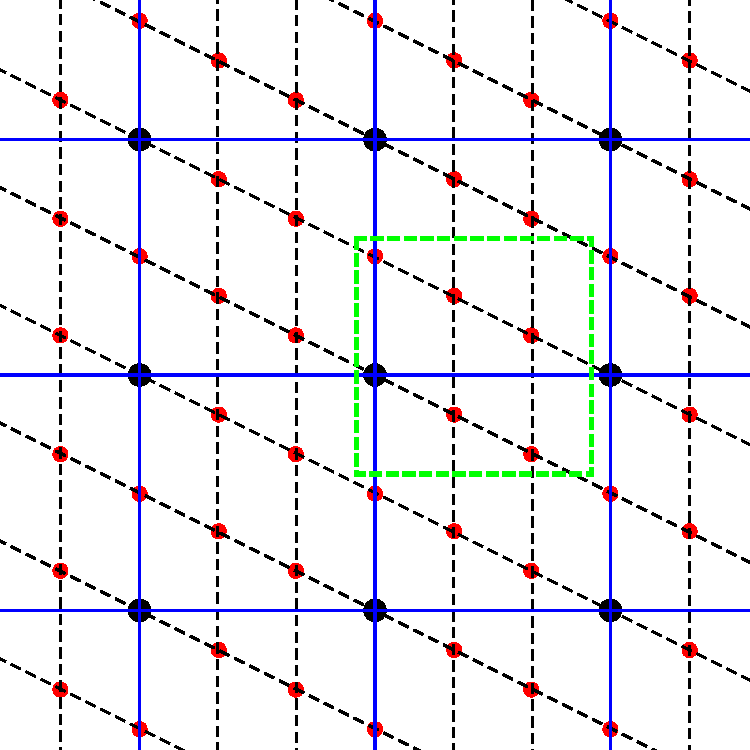
\includegraphics[width=0.40\textwidth]{HLReciprocalLattice2}
  \caption{\label{fig:HLReciprocalLattice2}
(Color online)
The reciprocal lattices of both the Bravais lattice $\Lambda$ and the
integer square lattice. The red points are the reciprocal lattice $\Lambda^*$ of the Bravais
lattice $\Lambda$ in \reffig{fig:BravaisLatt}. The black points are
the reciprocal lattice of the square lattice. Each of these squares
enclosed by the blue lines has edge length $2 \pi$.
%And these squares are also repeating unit of the wave vectors (the red dots in this figure).
Two wave vectors are equivalent if they are different by a
reciprocal lattice vector of the square lattice.
}
\end{figure}
%%%%%%%%%%%%%%%%%%%%%%%%%%%%%%%%%%%%%%%%%%%%%%%%%%%%%%%%%%%%%%%



\subsection{Backup from s previous version of \catlatt}

The set of all wave vectors $\mathbf{K}_m$ that yield plane waves with
the periodicity of a given Bravais lattice defines its reciprocal
lattice. The $\mathbf{K}_m$ are called reciprocal lattice vectors.

% from Barvinok \arXiv{/math/0504444}:
Let $\langle \cdot, \cdot \rangle$ be the scalar product on $\reals^d$.
% and the corresponding Euclidean norm $\| \cdot\|$.
Let $\Lambda \subset\reals^d$ be a lattice,
and let  $\Lambda^{\ast} \subset\reals^d$ be its {\it reciprocal} lattice
\beq
\Lambda^{\ast}=
\Bigl\{x \in \reals^d: \quad \langle x, y \rangle \in {\Bbb Z} \quad
\mbox{for all} \quad y \in \Lambda
\Bigr\}\,.
\ee{dualLatt}

The reciprocal lattice of the Bravais lattice \refeq{2DBravaisLattice} is
spanned by reciprocal basis \refeq{RecLattBasis}
\beq
\Lambda^* = \{n_1 \mathbf{b}_1 + n_2 \mathbf{b}_2\,|\,n_i \in \mathbb{Z}\}
\,.
\ee{2DReciprocalLattice}
The eigenvectors of the translation operator have the form
of a plane wave
\beq
f_{k}({z})
= e^{i {k} \cdot {z}} \, , \quad {k} \in \Lambda^*
\,,
\ee{2DEigenvectors}
and, in addition, satisfy the Bravais lattice \refeq{2DBravaisLattice}
periodicity.



Then the basis vectors of the reciprocal lattice are:
\beq
\left[
\begin{array}{cc}
\mathbf{b}_1 & \mathbf{b}_2 \\
\end{array}
\right]
=
\frac{2 \pi}{\speriod{} \period{}}
\left[
\begin{array}{cc}
 \period{} & 0 \\
 -{S} & \speriod{} \\
\end{array}
\right]
 \, .
\ee{2DReciprocalBasis}
A plane wave with wave vector $\mathbf{k}$ in
the reciprocal lattice $\Lambda^*$ is an eigenvector of the
{\jacobianOrb} \refeq{dDCatsT} that satisfies the periodic condition of
Bravais lattice $\Lambda$. The eigenvector with wave vector
$\mathbf{k}=n_1\mathbf{b}_1+n_2\mathbf{b}_2$ is
\beq
f_{k}({z}) = e^{i {k} \cdot {z}}
  = \exp\left(
      i\frac{2 \pi}{\speriod{} \period{}}(n_1 \period{} z_1 - n_1 {S} z_2 + n_2 \speriod{} z_2)
        \right)
\,,
\ee{2DEigenvector}
where the ${z}=(z_1,z_2)$, with the {\jacobianOrb}  eigenvalue
\beq
\lambda_{k}
= \sum_{j=1}^2 ({s} - 2 \cos k_j)
= 2s - 2 \cos2\pi(\frac{n_1}{\speriod{}})
    - 2 \cos2\pi(\frac{n_1 {S}}{\speriod{} \period{}}
                -\frac{n_2}{\period{}})
\,.
\ee{2DEigenvalue}
As the field has support on the square lattice sites, it suffices to use
the wave vectors
$\mathbf{k}= n_1 \mathbf{b}_1 + n_2 \mathbf{b}_2$
with $n_1$ from 0 to $\speriod{}-1$ and $n_2$ from 0 to $\period{}-1$ to
get all the reciprocal lattice eigenvectors.
    \PC{2020-05-28}{Perhaps use
\[
\cos(a-b) = \cos(a)\cos(b) + \sin(a)\sin(b)
\,?
\]
\[
\cos(2a) = \cos(a)^2 - \sin(a)^2 = 1 - 2\sin(a)^2
\,?
\]
\[
{s}-2\cos k_1  = ({s}-2) + 4(\sin(k_1/2))^2
\]
\[
{s}-2\cos k_2  = ({s}-2) + 4(\sin(k_1/2))^2
\]
Set \(q_1=2\pi{k_1}/{\speriod{}}\,,\)
\(q_2=2\pi{k_2}/{\period{}}\,,\)
\(C=\speriod{}/{\period{}}\,,\)
\[
2\cos(q_2-Cq_1) = 2\cos(q_2)\cos(Cq_1) + 2\sin(q_2)\sin(Cq_1)
\]
    }

This range contains all of the wave vectors in one lattice cell of
reciprocal lattice of the square lattice, as shown in
\reffig{fig:HLReciprocalLattice2}, where wave vectors with $n_1$ from 0
to $\speriod{}-1$, and $n_2$ from 0 to $\period{}-1$ are enclosed by the
green dashed square. Any wave vector on the reciprocal lattice
$\Lambda^*$ outside of this range will give an eigenvector which is
equivalent to an eigenvector with the wave vector within this range. So
the number of eigenvectors is $\speriod{} \period{}$, which is the number
of square lattice sites within the minimal repeating tile.

The 4-index {\jacobianOrb} \refeq{dDCatsT} is a matrix with indices in a
finite range. The {\jacobianOrb} has $\speriod{}\period{}$ eigenmodes. We
know that the number of {\twots} is equal to the {\HillDet} of the
{\jacobianOrb}, which is the product of all the eigenvalues,
% $N_{\LTS{}{}{}}=\prod_{k}\lambda_{k}$,
\beq
N_{\LTS{}{}{}}
=  2^{\speriod{}\period{}}\prod_{k_1=0}^{\speriod{}-1} \prod_{k_2=0}^{\period{}-1}
     \left[s  -  \cos\left(\frac{2\pi k_1}{\speriod{}}\right)
              -  \cos\left(
                            \frac{2\pi k_2}{\period{}}
                           -\frac{2\pi k_1}{\speriod{}}
                            \frac{ \tilt{}}{\period{}}
                     \right)
     \right]
%.
\label{2DCountingFormula}
\eeq

Given the eigenmodes with a given periodic condition, one can reduce the
2\dmn\ square lattice to a finite repeating tile. The {\sPe} in this tile
is still \refeq{dDCatsT}. But now the fields and sources are defined over an
$\LTS{}{}{}$ lattice.

\beq
N_{\BravCell{1}{1}{0}} =  2s - 4 = 1
 \,.
\label{1x1DCount}
\eeq

\beq
N_{\BravCell{\speriod{}}{1}{0}}
=  \prod_{k_1=0}^{\speriod{}-1}
     \left[2s_2 - 2 - 2 \cos\left(\frac{2\pi k_1}{\speriod{}}\right)
     \right]
 \,.
\label{2Dto1DCount}
\eeq
Comparing with the \templatt\ count \refeq{appe:detTemCatCheb} we see
that the count is the same, provided we replace
\(
{s}_1\to2({s}_2-1)
\,,
\)
in agreement with the 3-term recurrence \refeq{eq:CatLattT=1}.


\subsubsection{$\BravCell{2}{1}{1}$ \twots.}
\label{s:catLatt2x2rel1}
%    \HLpost{2019-11-22}{
For $s=5/2$ \catlatt.
\beq
N_{\BravCell{2}{1}{1}}
= \prod_{l=0}^{1}
  \Big[
  2s - 4 \cos2\pi\left(\frac{l}{2}\right)
  \Big]
= 9
 \,.
\ee{2x1_1Fourier}

\subsubsection{$\BravCell{2}{2}{0}$ \twots.}
\label{s:catLatt2x2}
For $s=5/2$ \catlatt.
\[
N_{[2\!\times\!2]} =
2^4({s}- 2)({s}- \cos\pi -1)({s}- 1 - \cos\pi)({s}- \cos\pi - \cos\pi) = 225
\,.
\]

\subsubsection{$\BravCell{3}{2}{0}$ \twots.}
\label{s:catLattRel3x2}
%    \HLpost{2019-11-23}{
For $s=5/2$ only 850 prime $\BravCell{3}{2}{0}$ \brick s are \admissible. The
integer points count \refeq{HL[3x2]count} is in agreement with the
counting formula \refeq{2DCountingFormula} for the $\BravCell{3}{2}{0}$
\twots:
     \[
N_{\BravCell{3}{2}{0}}
  = \prod_{l=0}^2\prod_{t=0}^1\left[
  2{s}-2\cos\left(\frac{2 \pi l}{3}\right)-2\cos\left(\frac{2 \pi t}{2}\right)
                              \right]
  = 5120
     \,.
     \]

%%%%%%%%%%%%%%%%%%%%%%%%%%%%%%%%%%%%%%%%%%%%%%%%%%%%%%%%%%%%%%%%%%%%%%%
\renewcommand{\statesp}{phase space}
\renewcommand{\Statesp}{Phase space}
\renewcommand{\stateDsp}{phase-space}
\renewcommand{\StateDsp}{Phase-space}

    \ifboyscout\clearpage\fi
% siminos/kittens/appeBernoulli.tex      pdflatex CL18
% $Author: predrag $ $Date: 2020-06-03 08:40:39 -0500 (Wed, 03 Jun 2020) $

\section{Temporal Bernuolli}
\label{appe:1D1dLatt}

\renewcommand{\statesp}{state space}
\renewcommand{\Statesp}{State space}
\renewcommand{\stateDsp}{state-space}
\renewcommand{\StateDsp}{State-space}

Applied to a temporal lattice state \Xx\ of period \cl{}, the {\shiftOp}
%\refeq{shiftBern},
\refeq{hopMatrix} acts as a cyclic permutation that
translates the lattice state $\Xx$ by one site, $\transp{(\hopMat
\Xx)}=(\ssp_2,\ssp_3, \cdots, \ssp_\cl{},\ssp_1)$, with `1' in the lower
left corner assuring periodicity.
\index{cyclic!permutation matrix}

After $\cl{}$ shifts, the lattice state \Xx\ returns to the initial
state, $\hopMat^\cl{}=\unit$. This relation leads to the explicit expression for
the orbit {\jacobianM} \refeq{tempBernGreen},
\beq
\gd
    =  \frac{\hopMat}{s\,\unit-\hopMat}
    = \frac{1}{\unit-\frac{\hopMat}{s}}\,\frac{\hopMat}{s}
    = \sum_{k=1}^\infty \frac{\hopMat^k}{s^k}
%    =  \sum_{m=0}^\infty \frac{1}{s^{\cl{}m}}
%      \sum_{k=1}^\cl{} \frac{\hopMat^k}{s^k}
    =  \frac{s^\cl{}}{s^\cl{} - 1}
      \sum_{k=1}^\cl{} \frac{\hopMat^k}{s^k}
\,.
\ee{appe:BernGreenFct}
From \refeq{tempBernGreen} it then follows that the last field in
$\Xx$ is the field at lattice site $\cl{}$
\beq
\ssp_{\cl{}}
=  \frac{s^\cl{}}{s^\cl{} - 1}
          .\Ssym{1}\Ssym{2}\Ssym{3}\cdots\Ssym{\cl{}}
=  \frac{1}{s - 1}\,%\sum_{k=1}^\cl{} \Ssym{k} 2^{\cl{}-k}
    \frac{s^{\cl{}-1}\Ssym{1}+\cdots+s\,\Ssym{\cl{}-1}+\Ssym{\cl{}}}
         {s^{\cl{}-1}+\cdots+s+1}
\,,
\label{appe:Bern_cyc}
\eeq
and the rest are obtained by cyclic permutations of $\Mm$.

% from ChaosBook \Chapter{appendKnead}
% \section{Pruned Bernoulli shift} \label{sect:PrunBernoulli}
For example, for ${s}=2$, the lattice fields are rational-valued,
\bea
\ssp_{\Ssym{1}\Ssym{2}\cdots \Ssym{n}}
&=&  \sum_{k=1}^\cl{} \frac{\Ssym{k}}{2^k} \sum_{m=0}^\infty \frac{1}{2^{\cl{}m}}
        = \frac{2^\cl{}}{2^\cl{} - 1} .\Ssym{1}\Ssym{2}\cdots \Ssym{\cl{}}
\continue
&=& \frac{1}{2^\cl{} - 1}\,\sum_{k=1}^\cl{} \Ssym{k} 2^{\cl{}-k}
\,,
\label{Bern_cyc1}
\eea
where $p=\overline{\Ssym{1}\Ssym{2}\cdots \Ssym{\cl{}}}$ is a prime cycle of period
\cl{}, with stability multiplier $\ExpaEig_p=2^\cl{}$.

For a Bernoulli map,
the rational $\ssp_{0}$ are either periodic or land eventually on a \po\
(the base-${s}$ version of the familiar fact that the decimal expansion
of a rational number is eventually periodic), while the orbit of a normal
irrational $\ssp_{0}$ is ergodic.
    \PC{2019-07-30}{
Since all coefficients in \refeq{OneCat} are integers, the lattice states
$\ssp_\zeit$  are always rational. This allows for their exact evaluation
by integer arithmetic.
    }

    \ifboyscout\clearpage\fi
% siminos/kittens/catHamilton.tex                   pdflatex CL18
% $Author: predrag $ $Date: 2020-07-28 01:02:24 -0500 (Tue, 28 Jul 2020) $

\section{Cat map: Hamiltonian formulation}
\label{s:catMapHam}
    % earlier names:
    % siminos/spatiotemp/chapter/catHamilton.tex
    % \section{Life of a single Hamiltonian cat}

\subsection{\AW\ partition of the cat map \statesp}
\label{s:catAW}

%%%%%%%%%%%%%%%%%%%%%%%%%%%%%%%%%%%%%%%%%%%%%%%%%%%%%%%%%%%%%
% PC 2018-02-09 PVAdlerWeissB-a.svg started from PCLect13p9.svg
% PC 2018-02-09 PVAdlerWeissB-b.svg started from PCLect13p15.svg
% PC 2018-02-09 PVAdlerWeissB-c.svg started from PCLect13p16a.svg
% PC 2018-02-09 PVAWMarkov.svg B&W started from Lect13p17.pdf
% PC 2018-02-11 PVAWMarkovCol.svg  started from PVAWMarkov.svg
%               bit too big - redraw from scratch
\begin{figure}\begin{center}
            \begin{minipage}[c]{0.23\textwidth}\begin{center}
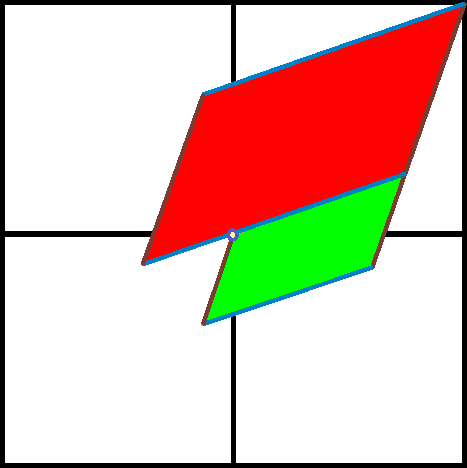
\includegraphics[width=1.0\textwidth]{PVAdlerWeissB-a}\\(a)
            \end{center}\end{minipage}
            \begin{minipage}[c]{0.23\textwidth}\begin{center}
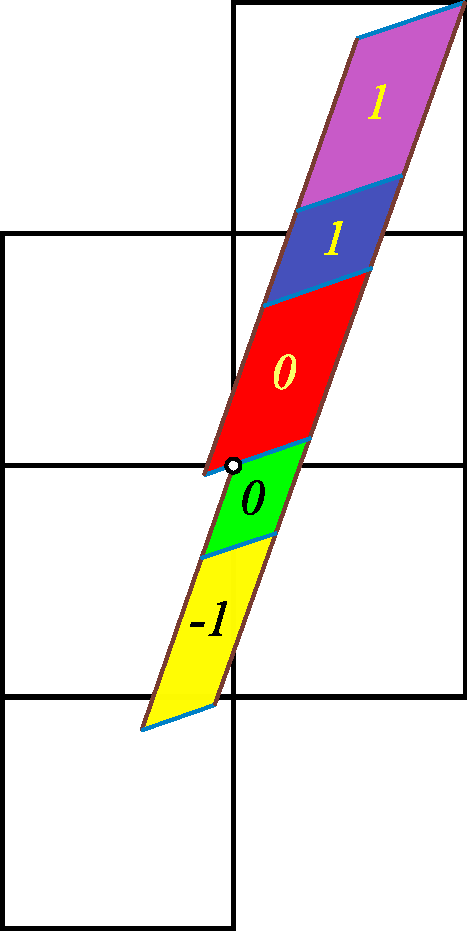
\includegraphics[width=1.0\textwidth]{PVAdlerWeissB-b}\\(b)
            \end{center}\end{minipage}
            \begin{minipage}[c]{0.23\textwidth}\begin{center}
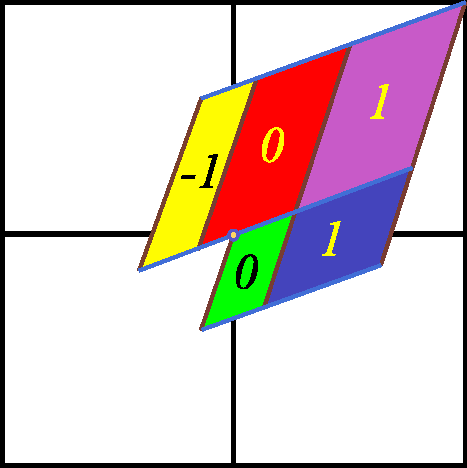
\includegraphics[width=1.0\textwidth]{PVAdlerWeissB-c}\\(c)
            \end{center}\end{minipage}
            ~~~
            \begin{minipage}[c]{0.12\textwidth}\begin{center}
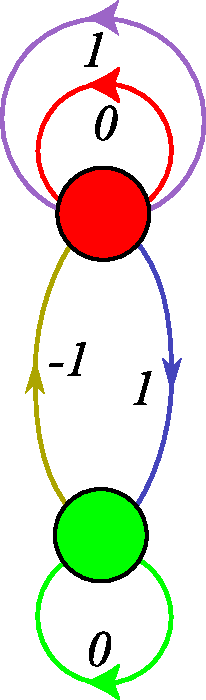
\includegraphics[width=1.0\textwidth]{PVAWMarkovCol}\\(d)
            \end{center}\end{minipage}
\end{center}
  \caption{\label{fig:PVAdlerWeiss}
(Color online)
(a)
An \AW\ generating partition of the unit torus for the $s=3$ \PV\ cat map
\refeq{eq:StateSpCatMap}, with rectangle $\pS_A$ (red) and $\pS_B$
(green) borders given by the cat map stable (blue) and unstable (dark
red) manifolds, \ie, along the two eigenvectors corresponding to the
eigenvalues \refeq{StabMtlpr}.
(b)
Mapped one step forward in time, the rectangles are stretched along the
unstable direction and shrunk along the stable direction. Sub-rectangles
$\pS_j$ that have to be translated back into the partition are indicated by
color and labeled by their lattice translation
$\Ssym{j}\in\A=\{\underline{1},0,1\}$, which also doubles as the 3-letter
alphabet $\A$.
(c)
The sub-rectangles $\pS_j$ translated back into the initial partition
yield a generating partition, with the finite grammar given by the
{\markGraph}
(d).
The nodes
refer to the rectangles $A$ and $B$, and the five links correspond to the five
sub-rectangles induced by one step forward-time dynamics.
For details, see ChaosBook\rf{DasBuch}.
% make ChaosBook link specific.
}
\end{figure}
%%%%%%%%%%%%%%%%%%%%%%%%%%%%%%%%%%%%%%%%%%%%%%%%%%%%%%%%%%%%%%%

Cat maps, also known as Thom-Anosov diffeomorphisms, or
Thom-Anosov-Arnol'd-Sinai {cat maps}\rf{ArnAve,deva87,StOtWt06}, have
been extensively studied as the simplest examples of chaotic Hamiltonian
systems.

\PV\ cat map \refeq{eq:StateSpCatMap} is a discrete time non-autonomous
Hamiltonian system, time-forced by `pulses' $\Ssym{\zeit}$.
The $\Ssym{\zeit}$ translations reshuffle the \statesp, as in
\reffig{fig:PVAdlerWeiss}, thus partitioning it into regions
$\pS_\Ssym{}$, labeled with letters $\Ssym{}$ of the $|\A|$-letter
alphabet $\A$, and associating a symbol sequence $\{\Ssym{\zeit}\}$ to
the dynamical trajectory $\{\ssp_{\zeit}\}$. As the relation
\refeq{eq:StateSpCatMap} between the trajectory \(\ssp_{\zeit}\) and its
symbolic dynamics encoding \(\m_{\zeit}\) is linear, Percival and Vivaldi
refer to \(\m_{\zeit}\) as a `linear code'.

As explained in the companion paper\rf{GHJSC16},
the deep problem with the \PV\ code prescription is that it does not
yield a generating partition; the borders (\ie, $\ssp_0$, $\ssp_1$ axes)
of their unit-square partition
$(\ssp_{\zeit-1},\ssp_{\zeit})\in(0,1]\times(0,1]$
do not map onto themselves, resulting in the infinity of, to us unknown,
grammar rules for {\inadmissible} symbol sequences.

This problem was resolved in 1967 by Adler and
Weiss\rf{AdWei67,ArnAve,AdWei70} who utilized the stable/\-unstable
manifolds of the fixed point at the origin to cover a unit area torus by
a two-rectangles generating partition; for the \PV\ cat map
\refeq{eq:StateSpCatMap}, such partition\rf{DasBuch} is drawn in
\reffig{fig:PVAdlerWeiss}. Following Bowen\rf{Bowen70}, one refers to
parallelograms in \reffig{fig:PVAdlerWeiss} as `rectangles'; for details
see Devaney\rf{deva87}, Robinson\rf{Robinson12}, or
ChaosBook\rf{DasBuch}. Siemaszko and Wojtkowski\rf{SieWoj11} refer to
such partitions as the `Berg partitions', and Creagh\rf{Creagh94} studies
their generalization to weakly nonlinear mappings. Symbolic dynamics on
this partition is a subshift of finite type, with the 3-letter alphabet
\beq
\A=\{\underline{1},0,1\}
\ee{catAlphabetPVAW}
that indicates the translation needed to return the given sub-rectangle
$\pS_{{j}}$ back into the two-rectangle partition $\pS= \pS_{{A}}\cup
\pS_{{B}}$.

While Percival and Vivaldi were well aware of \AW\ partitions, they felt
that their ``coding is less efficient in requiring more symbols, but it
has the advantage of linearity.'' Our construction demonstrates that one
can have both:  an \AW\ generating cat map partition, and a linear code.
The only difference from the \PV\ formulation\rf{PerViv} is that one
trades the single unit-square cover of the torus of
\refeq{eq:StateSpCatMap} for the dynamically intrinsic, two-rectangles
cover of \reffig{fig:PVAdlerWeiss}, but the effect is magic - now every
infinite walk on the {\markGraph}  of \reffig{fig:PVAdlerWeiss}\,(d)
corresponds to a unique {\admissible} orbit $\{\ssp_{\zeit}\}$, and the
{\markGraph} generates all {\admissible} itineraries $\{\Ssym{\zeit}\}$.

To summarize:
an explicit \AW\ generating partition, such as
\reffig{fig:PVAdlerWeiss}, completely solves the Hamiltonian cat map
problem, in the sense that it generates all {\admissible} orbits.
Rational and irrational initial states generate periodic and ergodic
orbits, respectively\rf{PerViv87b,Keating91}, with every \statesp\ orbit
uniquely labeled by an {\admissible} bi-infinite itinerary of symbols
from alphabet \A.

\subsection{Counting Hamiltonian cat map \po s}
\label{s:catHamCount}

                                \toCB
    %\PC{2019-08-01}{
The five sub-rectangles $\pS_{{j}}$ of the two-rectangle \AW\ partition
of \reffig{fig:PVAdlerWeiss}\,(c) motivate introduction of a 5-letter
alphabet
\beq
\Aa=\{ {1}, {2}, {3}, {4}, {5}\}
  = \{A{}^0\!A, B{}^1\!A, A{}^1\!A, B{}^0\!B, A{}^{\underline{1}}\!B\}
\,,
\ee{cat5AlphabetPVAW}
see \reffig{fig:PVAdlerWeissS}\,(b), which encodes the links of the
{\markGraph}  of \reffig{fig:PVAdlerWeiss}\,(d). The loop expansion  of
the determinant\rf{CBcount} of the {\markGraph} $T$ of
\reffig{fig:PVAdlerWeissS}\,(b)  is given by all non-intersecting walks
on the graph
\beq
\det(1-zT) = 1 - z(t_1+t_3+t_4)
               - z^2 (t_{25}-(t_1+t_3)t_4)
 \,,
\ee{CatMapDetTransMat}
where $t_p$ are traces over fundamental cycles, the three fixed points
\(
t_1 = T_{A{}^0\!A},
t_3 = T_{A{}^1\!A},
t_4 = T_{B{}^0\!B},
\)
and the 2-cycle
\(
t_{25} = T_{B{}^{1}\!A} T_{A{}^{\underline{1}}\!B}
\,.
\)

As the simplest application, consider counting all {\admissible} cat map
\po s. This is accomplished  by setting the non-vanishing links of the
{\markGraph} to $T_{ji}=1$, resulting in the ${s}=3$ cat map
\tzeta\rf{Isola90,DasBuch},
\beq
\zetatop(z) =  \frac{1 - 3 z + z^2}
                  {(1 - z)^2}
\,,
\ee{Isola90-13a}
where the numerator ${(1 - z)^2}$ corrects the overcounting of the fixed
point at the origin due to assigning it to both $\pS_A$ (twice) and
$\pS_B$ rectangles\rf{manning}.

    \PC{2020-02-08}{
Note:
$N_2=\Det\jMorb=({s}-2)({s}+2)$,
$N_3 %   = {s}^3-3{s}-2
    = ({s}-2)({s}+1)^2$,
$N_4 = ({s}-2)({s}+1)\,{s}^2$,
$N_5 = ({s}-2)(s^2+ s-1 )^2$.
I think the factorization is true for all $\cl{}$, as the $s=2$ Laplacian
has a zero mode (constant $\ssp_i$, I think).

an sequence of non-negative integers counting the orbits of
a map; the sequence of periodic points for that map.
    }


%    \PCpost{2020-01-16}
                               \toCB
The number of \emph{periodic points} of
period $n$ is given by \refeq{zetatop-N}, the logarithmic derivative of
the {\tzeta}. Substituting the cat map \tzeta\ \refeq{Isola90-13a} we
obtain
% ------------------- siminos/mathematica/ ----------
% CatMaptopZeta.nb                                    2020-01-16
%    Cat map periodic points counting for CL18.tex
% 1,5,16,45,121,320,841,2205,5776,15125,39601,
\bea
\sum_{n=1}N_n z^n
    &=&
 z+5 z^2+16 z^3+45 z^4+121 z^5+320 z^6+841 z^7
    \ceq
+2205 z^8+5776 z^9+15125 z^{10}
+39601 z^{11}
+\cdots
%+O\left(z^{11}\right)
\label{catMapN_n-s=3}
\eea
WolframAlpha says, compare with \refeq{1stChebGenF}:
\beq
\sum_{n=1}N_n z^n % = \frac{-z - 1}{z^3 - 4 z^2 + 4 z - 1}
            % = \frac{-z - 1}{(z - 1) (z^2 - 3 z + 1)}
            = \frac{s - 2 z}{1 - s z + z^2} - \frac{2}{1 - z}
\ee{s=3PPs}

The number of \emph{prime} cycles is given by
\refeq{primeCount},
% ------------------- siminos/mathematica/ ----------
% CatMaptopZeta.nb                                    2020-01-16
%    Cat map periodic points counting for CL18.tex
% 1,2,5,10,24,50,120,270,640,1500,3600,...
% see https://oeis.org/A032170 https://oeis.org/A072337
%     https://oeis.org/A004146/internal
% a(n) = 2*(T(n, 3/2)-1)with Chebyshev's polynomials T(n, x) of the first kind.
%        See their coefficient triangle https://oeis.org/A053120
% a(n) = 2*T(n, 3/2) - 2, with twice the Chebyshev's polynomials of the first kind,
%                           2*T(n, x=3/2)= https://oeis.org/A005248
\bea
\sum_{n=1}M_n z^n
    &=&
 z+2 z^2+5 z^3+10 z^4+24 z^5+50 z^6+120 z^7
    \ceq
+270 z^8+640 z^9+ 1500z^{10}+3600 z^{11}
+\cdots
% +O\left(z^{11}\right)
\,,
\label{catMapM_n-s=3}
\eea
in agreement with the Bird and Vivaldi\rf{BirViv} census.
% (they call that $N_T(\lambda)$ in their Table~1, with $s=K=3$ and $4$),

%%%%%%%%%%%%%%%%%%%%%%%%%%%%%%%%%%%%%%%%%%%%%%%%%%%%%%%%%%%%%
\begin{figure}\begin{center}
            \begin{minipage}[c]{0.30\textwidth}\begin{center}
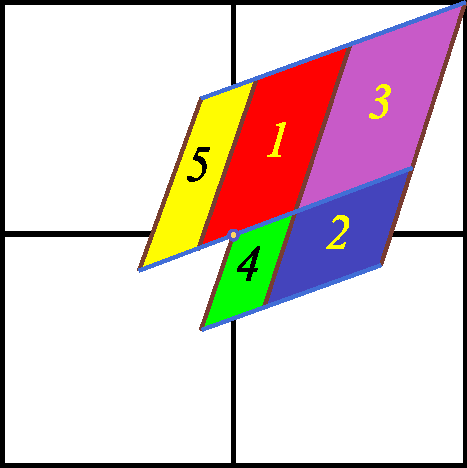
\includegraphics[width=1.0\textwidth]{PVAdlerWeissS-c}\\(a)
            \end{center}\end{minipage}
            \hskip 8ex
            \begin{minipage}[c]{0.12\textwidth}\begin{center}
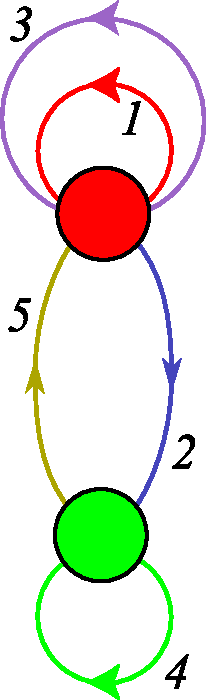
\includegraphics[width=1.0\textwidth]{PVAWMarkovSymb}\\(b)
            \end{center}\end{minipage}
\end{center}
  \caption{\label{fig:PVAdlerWeissS}
(Color online)
(a)
The sub-rectangles $\pS_j$ of \reffig{fig:PVAdlerWeiss}\,(c).
(b)
Admissible orbits correspond to walks on the {\markGraph} of
\reffig{fig:PVAdlerWeiss}\,(d), with rectangles $\pS_A$ (red) and
$\pS_B$ (green) as nodes, and the links labeled by
5-letter alphabet \refeq{cat5AlphabetPVAW}, see the
loop expansion \refeq{CatMapDetTransMat}.
}
\end{figure}
%%%%%%%%%%%%%%%%%%%%%%%%%%%%%%%%%%%%%%%%%%%%%%%%%%%%%%%%%%%%%%%

%%%%%%%%%%%%%%%%%%%%%%%%%%%%%%%%%%%%%%%%%%%%%%%%%%%%%%%%%%%%%%%
\begin{figure}
  \centering
(a)   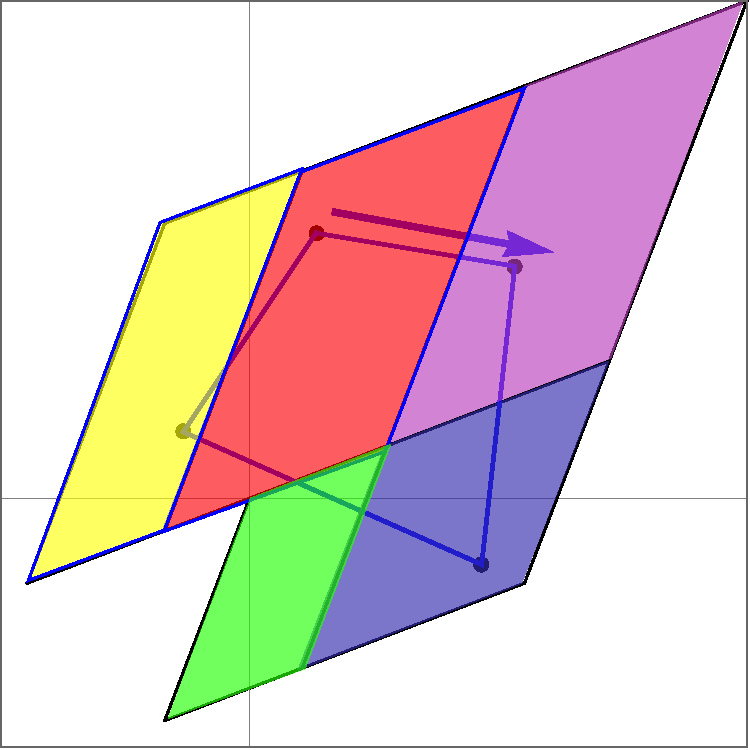
\includegraphics[width=0.35\textwidth]{HLPeriodicOrbit5}
\hskip 1ex
(b)   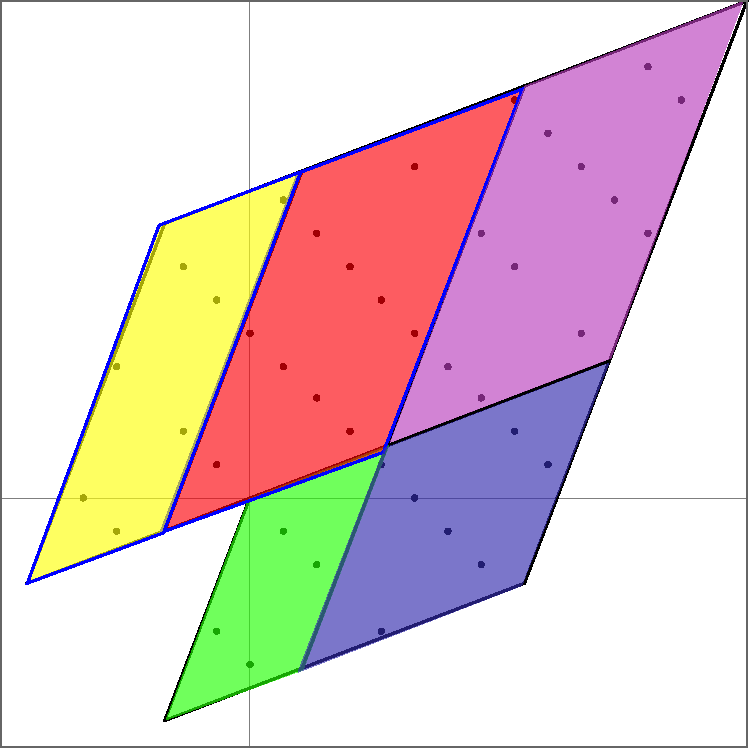
\includegraphics[width=0.35\textwidth]{HLAllCyclePointsB}
      % from \reffig{fig:HLAllCyclePoints}
 	\caption{\label{fig:HLPeriodicOrbitsA}
(a) An example of a 4-cycle:
$\Xx_{0 1 1 \underline{1}}$. %\frac{1}{15}(2,8,7,-2)$,
(b) All prime period-4 lattice states land in the partition of
\reffig{fig:PVAdlerWeissS}\,(a).
% Added colors to these two figures so readers can compare the orbit
% with the transition graph \reffig{fig:PVAdlerWeissS} (b).
}
\end{figure}
%%%%%%%%%%%%%%%%%%%%%%%%%%%%%%%%%%%%%%%%%%%%%%%%%%%%%%%%%%%%%%%

This derivation was based on the \AW\ generating partition, a clever
explicit visualization of the cat map dynamics, whose generalization to
several coupled maps (let alone spatially infinite coupled cat
maps lattice) is far from obvious: one would have to construct covers of
high-dimensional {\fundPip}s by sets of sub-volumes.
However, as Keating\rf{Keating91} explains, no such explicit generating
partition is needed to count cat map \po s.
Cat map \refeq{eq:StateSpCatMap} lattice states are the fixed points of
\[
\left[\begin{array}{c}
  \coord_\zeit  \\ p_\zeit
  \end{array}\right]
=
   \left[\begin{array}{c}
  \coord_{\zeit+\cl{}}  \\ p_{\zeit+\cl{}}
  \end{array}\right]
=
  \jMps^\cl{}
  \left[\begin{array}{c}
  \coord_\zeit  \\ p_\zeit
  \end{array}\right]
  \quad (\mbox{mod}\;1)
\,,
\]
so on the unwrapped phase space lattice, tiled by repeats of the
unit square of the cat map torus,
\beq
 (\jMps^\cl{} - \matId)
    \left[\begin{array}{c}
 \coord_\zeit  \\ p_\zeit
    \end{array}\right]
=
    \left[\begin{array}{c}
m_{\zeit}^\coord \\ m_{\zeit}^p
    \end{array}\right]
\,,\qquad
    (m_{\zeit}^\coord,m_{\zeit}^p)\in\integers^2
\,,
\ee{fundParallelo}
matrix $(\jMps^\cl{} - \matId)$ stretches the unit square into
the `{\fundPip}'.

\subsection{An example: period-4 prime cycles}
\label{s:cat4cycles}

% \PCpost{2018-02-11}{
As a hands-on example, let us count the $M_4=10$ {\admissible} prime
4-cycles, as stated in \refeq{noPrimeCycs=3}.
The {\admissible} \brick s $\Mm_p$ can be read off as walks on
either the 5-letter alphabet \refeq{cat5AlphabetPVAW} graph, see
\reffig{fig:PVAdlerWeissS}\,(b),
or the 3-letter alphabet \refeq{catAlphabetPVAW} graph, see
\reffig{fig:PVAdlerWeiss}\,(d). They are, in 5-letter (top), and
3-letter (bottom) alphabets
        \PC{2019-12-20}{
For covering symbolic dynamics, use/refer to ChaosBook.

Order \refeq{prime4cycles} lexically.
    }

\bea
&&
\begin{array}{c} \cycle{1113} \\  0 0 0            1 \end{array} \;
\begin{array}{c} \cycle{1125} \\  0 0 1 \underline{1}\end{array} \;
\begin{array}{c} \cycle{1245} \\  0 1 0 \underline{1}\end{array} \;
\begin{array}{c} \cycle{1253} \\  0 1 \underline{1}1 \end{array} \;
\begin{array}{c} \cycle{1325} \\  0 1 1 \underline{1}\end{array} \;
        \continue
&&
\begin{array}{c} \cycle{1133} \\  0 0 1            1 \end{array} \;
\begin{array}{c} \cycle{3325} \\  1 1 1 \underline{1}\end{array} \;
\begin{array}{c} \cycle{3331} \\  1 1 1            0 \end{array} \;
\begin{array}{c} \cycle{3245} \\  1 1 0 \underline{1}\end{array} \;
\begin{array}{c} \cycle{4452} \\  0 0 \underline{1}1 \end{array}
\,.
\label{prime4cycles}
\eea
% with the corresponding overall translation per cycle given by
% the sum of the 3-letter alphabet labels.

% \HLpost{2018-02-11}{
The corresponding \po s $\Xx_p$ are computed using Green's function
\refeq{1dLatGreenFct} (the inverse of the $[4\times4]$ {\jacobianOrb} \refeq{Hessian},
easiest to evaluate by discrete Fourier transforms, see
\refappe{appe:Fourier}):
\[
\Mm_{0 0 0 1}
            \Rightarrow\quad
\Xx_{0 0 0 1}= g
\left[\begin{array}{c}
 0 \\
 0 \\
 0 \\
 1 \\
\end{array}\right]
   =
\frac{1}{15}
\left[\begin{array}{c}
 {3} \\
 {2} \\
 {3} \\
 {7} \\
\end{array}\right]
\,.
\]
Likewise,
        \PC{2019-12-20}{
To Han: order lexically.
    }

\bea
\transp{\Xx}_{0 0 1 \underline{1}} &=& \frac{1}{15}
\left[\begin{array}{cccc}
 {-1} &
 {1} &
 {4} &
 {-4}
\end{array}\right]
    \,,\qquad
\transp{\Xx}_{0 1 0 \underline{1}}= \frac{1}{15}
\left[\begin{array}{cccc}
 {0} &
 {5} &
 {0} &
 {-5}
\end{array}\right]
    \continue
\transp{\Xx}_{0 1 \underline{1}1} &=& \frac{1}{15}
\left[\begin{array}{cccc}
 {4} &
 {6} &
 {-1} &
 {6}
\end{array}\right]
    \,,\qquad~~
\transp{\Xx}_{0 1 1 \underline{1}}= \frac{1}{15}
\left[\begin{array}{cccc}
 {2} &
 {8} &
 {7} &
 {-2}
\end{array}\right]
    \continue
\transp{\Xx}_{0 0 1 1} &=& \frac{1}{15}
\left[\begin{array}{cccc}
 {5} &
 {5} &
 {10} &
 {10}
\end{array}\right]
    \,,\qquad~~
\transp{\Xx}_{1 1 1 \underline{1}}= \frac{1}{15}
\left[\begin{array}{cccc}
 {9} &
 {11} &
 {9} &
 {1}
\end{array}\right]
    \continue
\transp{\Xx}_{1 1 1 0} &=& \frac{1}{15}
\left[\begin{array}{cccc}
 {12} &
 {13} &
 {12} &
 {8}
\end{array}\right]
    \,,\qquad
\transp{\Xx}_{1 1 0 \underline{1}}= \frac{1}{15}
\left[\begin{array}{cccc}
 {7} &
 {8} &
 {2} &
 {-2}
\end{array}\right]
    \continue
\transp{\Xx}_{0 0 \underline{1}1} &=& \frac{1}{15}
\left[\begin{array}{cccc}
 {1} &
 {-1} &
 {-4} &
 {4}
\end{array}\right]
\,.
\label{4-cyclePPs}
\eea
One can verify that for each of these 10 prime 4-cycles the  lattice
states $(\ssp_t,\ssp_{t+1})$ visit the rectangles $\pS_A$ or $\pS_B$ of
\reffig{fig:PVAdlerWeiss}\,(b) in the temporal order dictated by the
\markGraph, and thus they are all {\admissible} cycles.
    \PC{2020-01-28}{
Perhaps summarize here our failed efforts to make an time-reversal
invariant \AW\ partition; Ihara zeta functions, ...
    }

    \ifboyscout\clearpage\fi
% siminos/kittens/stab.tex  % called by CL18.tex
% $Author: predrag $ $Date: 2020-09-05 23:05:02 -0500 (Sat, 05 Sep 2020) $

\section{\Spt\ stability}
\label{s:stab}
% was siminos/spatiotemp/stability.tex  % called by blogCats.tex

\renewcommand{\deltaX}{\ensuremath{{\Delta \ssp}}}       %trajectory displacement

Here we address two questions:
(i) how is the high-dimensional orbit \jacobianM\ $\jMorb$ related
to the temporal [$d\!\times\!d$] \jacobianM\ $\jMps$?
and
(ii) how does one evaluate the orbit \jacobianM\ $\jMorb$?

\subsection{Temporal lattice}
\label{s:TempLatt}
% excerpted from \Chapter{cycles}{28sep2019}{Fixed points, and how to get them}
%

    \PCedit{
\beq
\jMorb_\Mm  = \unit-\jMps \otimes \hopMat^{-1}
\,,
\ee{dDmnForwardJacobianTMP}

the {temporal Bernoulli}
condition \refeq{tempBern} is the zero of function
\beq
F[\Xx;\Mm[ = \jMorb\Xx+\Mm = 0
\,,\qquad
\jMorb = \unit-{s}{\hopMat}^{-1}
\,,
\ee{tempBern-TMP}
    }

For a $d$\dmn\ discrete time map $\map$, with the lattice state $\Xx$ of
discrete period $\cl{}$, every temporal lattice site satisfies
\beq
\ssp_{\zeit+1}=\map(\ssp_\zeit)
\,,
\ee{CyclePntErr}
where $\ssp_\zeit$ is a $d$\dmn\ field at lattice site $\zeit$.
Consider an approximate lattice state, known only to a finite precision
\beq
\hat{\Xx}=(\hat{\ssp}_1,\hat{\ssp}_2,\cdots,\hat{\ssp}_\cl{})
\,,\quad
\hat{\ssp}_\zeit = \ssp_\zeit+\deltaX_\zeit
\,,
\ee{nXdCycleErr}
where $\ssp_\zeit$ is the exact field at lattice site \zeit.
Define the error field by
$F[\hat{\Xx}]=\map(\hat{\Xx})-\hopMat^{-1}\otimes\hat{\Xx}$, an operator
which compares the forward map of every point in $\hat{\Xx}$ with the
next point $\hat{\Xx}\otimes\hopMat$.

$F[\hat{\Xx}]$ is a $(\cl{}\!\times\!d)$\dmn\ temporal
lattice field obtained by stacking a $d$\dmn\ field $\hat{\ssp}_\zeit$ at
each of the $\cl{}$ lattice sites,
\beq
 F[\hat{\Xx}] \, = \, F
\left (
\begin{array}{l}
 \hat{\ssp}_1 \\ \hat{\ssp}_2 \\ \cdots \\ \hat{\ssp}_\cl{}
\end{array}
\right )
=
\left (
\begin{array}{l}
  \hat{\ssp}_1 - \hat{\map}_\cl{} \\ \hat{\ssp}_2 - \hat{\map}_1 \\
  ~~~\cdots \\ \hat{\ssp}_\cl{} - \hat{\map}_{\cl{}-1}
\end{array}
\right )
\,,\qquad \hat{\map}_\zeit = \map(\hat{\ssp}_\zeit)
\,,
\ee{errorVecs1D}
which measures the misalignment of every finite forward-in-time segment
$\map(\hat{\ssp})_\zeit$ with the next site $\hat{\ssp}_{\zeit+1}$ on the
lattice state $\hat{\Xx}$.

By \refeq{CyclePntErr}, the exact lattice state $\Xx$
% \refeq{nXdCycle}
is a zero of this vector field, $F[\Xx]=0$. Assuming that the $d$\dmn\
error vectors $\deltaX_\zeit$ are small in magnitude, and Taylor expanding the
{one discrete time-step} map $\map$ to linear order around the exact
solution,
\[
\map(\ssp_\zeit + \deltaX_\zeit)
   = \ssp_{\zeit+1} + \jMps_\zeit \deltaX_\zeit
    + (\cdots)
%\,,\qquad \map_\zeit = \map(\ssp_\zeit) = \ssp_{\zeit+1}
\,,
\]
where
\beq
[\jMps_\zeit]_{ij} = \frac{\pde \map_i(\ssp_\zeit)}{\pde \ssp_j}
    \,,\quad
\zeit
    = (1,2,\cdots,\cl{})
    \,,\quad
i,j
    \,=\, (1,2,\cdots,d)
\label{Hill:FntTimeJac}
\eeq
one finds that the neigh\-bor\-hood of entire cycle $p$ is
linearly deformed by the $[\cl{}d\times\cl{}d]$ orbit \jacobianM\
\beq
    \deltaX' = \jMorb(\ssp) \, \deltaX
    \,, \qquad
\jMorb_{ij}(\ssp)
  =  \frac{\delta F[\ssp]_i}{\delta \ssp_j}
\,,
\ee{stab:hOdes}
with
\[
{\cal J} \,=\,
1 - \hopMat \jMps
\,,
\]
the one discrete time-step temporal [$d\!\times\!d$] \jacobianM\
$\jMps$ evaluated on the entire cycle $p$, and $\hopMat$ the {\shiftOp}
\beq
\hopMat
= \left(
\begin{array}{cccccc}
%=\begin{bmatrix}
             0    &       &        &        &   &  \unit\cr
           \unit  &  0    &        &        &   &  \cr
                  & \unit &   0    &        &   &  \cr
                  &       & \unit  &        &  &  \cr
                  &       &        &   \ddots & 0 &  \cr
                  &       &        &        & \unit & 0
%        \end{bmatrix}
\end{array}
\right)
\,,\quad
\jMps
= \left(
\begin{array}{cccccc}
%=\begin{bmatrix}
          \jMps_1 &      &        &        &   &  \cr
                  & \jMps_2 &    &        &   &  \cr
                  &       &\jMps_3 &      &   &  \cr
                  &       &        & \ddots & &  \cr
                  &       &        & & \jMps_{\cl{}-1} &  \cr
                  &       &        &      &   & \jMps_{\cl{}}
%         \end{bmatrix}
\end{array}
\right)
\,,
\ee{shiftMatrix}
with $\unit$ in the upper right corner assuring periodicity,
$\hopMat^\cl{}=\unit$.

Consider a $d$-\dmn\ map $\ssp_{\zeit+1}=\map(\ssp_{\zeit})$, where
$\ssp_{\zeit}=\{\ssp_{\zeit,1},\ssp_{\zeit,2},\dots,\ssp_{\zeit,d}\}$ is
the state of the system at time $\zeit$. In case at hand, the one time step \jacobianM\
\beq
\jMps(\ssp_{\zeit})_{ij}
=
\left.\frac{\partial \map(\ssp)_i}{\partial \ssp_{j}}\right|_{\ssp_{i}=\ssp_{i,\zeit}}
%\,.
\ee{dDmn1stepJac}
stretches uniformly, so the \jacobianM\ does not depend on
the field value $\ssp_{\zeit}$ or time $\zeit$, $\jMps(\ssp_{\zeit}) =
\jMps$.

For a lattice state $\Xx_p$ with period $\cl{}$, the \jacobianOrb\ is a
$[\cl{}d\times\cl{}d]$ block matrix
\beq
\begin{array}{cc}
 \\ \\ \jMorb & = \\ \\
\end{array}
\left(
\begin{array}{ccccc}
\matId & & & & -\jMps \\
-\jMps & \matId & \\
& ~~\cdots~~ & \matId \\
 & & ~~\cdots~~ & \matId \\
 & & &-\jMps & \matId
\end{array}
\right)
= \unit-\jMps \otimes \hopMat^{-1}
\,,
\ee{dDmnForwardJacobian}
where \matId\ is a $d$-\dmn\ identity matrix, $\jMps$ is the
one time step $[d\times d]$ \jacobianM\ \refeq{dDmn1stepJac},
and $\hopMat$ is the $[\cl{}\times\cl{}]$ {\shiftOp} matrix with period $\cl{}$.

To evaluate the {\HillDet} of the \jacobianOrb, expand $\ln \Det \jMorb_p = \Tr \ln \jMorb_p$:
\bea
\ln \Det \jMorb_p
&=& \Tr \ln (\unit-\jMps \otimes \hopMat^{-1}) \continue
&=& - \sum_{k=1}^{\infty} \frac{\Tr (\jMps \otimes \hopMat^{-1})^k}{k}
\, .
\label{dDmnForwardJacobianLnDet}
\eea
Note that $(\jMps \otimes \hopMat^{-1})^k = \jMps^k \otimes \hopMat^{-k}$ and
$\Tr (\jMps^k \otimes \hopMat^{-k})
= \Tr (\jMps^{\cl{}r} \otimes \unit_{[\cl{}\times\cl{}]}) \delta_{k,\cl{}r}
= \cl{} \tr (\jMps^{\cl{}r}) \delta_{k,\cl{}r}
$
 which is not 0 only when $k$ is a multiple of $\cl{}$.
\bea
\ln \Det \jMorb_p
&=& - \sum_{r=1}^{\infty} \frac{\cl{} \tr (\jMps^{r\cl{}})}{r\cl{}}
 =  \tr [- \sum_{r=1}^{\infty} \frac{(\jMps^{\cl{}})^r}{r}] \continue
&=& \tr \ln (\unit - \jMps^{\cl{}})
 =  \ln \det (\unit - \jMps^{\cl{}})
\, .
\label{dDmnForwardJacobianLnDet2}
\eea
So the {\HillDet} of the \jacobianOrb\ is $\Det \jMorb = \det (\unit - \jMps^{\cl{p}})$.

\HL{2020-01-21}{
A possible problem is $\jMorb_p$ could be negative. And here we have the one time step
 \jacobianM\ instead of a scalar $s$ so I'm not sure if we can expand $\ln (\unit-\jMps \otimes \hopMat^{-1})$
 as a series in $\jMps \otimes \hopMat^{-1}$...
}


%%%%%%%%%%%%%%%%%%%%%%%%%%%%%%%%%%%%%%%%%%%%%%%%%%%%%%%%%%%%%
\subsection{Temporal stability}

% ``Hill's formula''
To summarize, a discretized, temporal lattice \po\ linear stability can
be computed in two ways - either by computing the
$[\cl{}d\times\cl{}d]$ {\jacobianOrb} $jMorb$, or by computing $\jMps_p$
\beq
\Det \jMorb_\Mm = \det (1-\jMps_\Mm)
\,,
\ee{dissipHill}
where $\jMps_\Mm$ is the $\cl{}$ time-steps $[d\!\times\!d]$ forward-time
\jacobianM. In the limit of discretization $\cl{}\to\infty$ the left
hand side is a {\em functional} {\HillDet} of an $\infty$\dmn\ {\em
operator}. Nevertheless, thanks to the discrete Fourier diagonalization
of $\jMorb(x)$, \refappe{appe:Fourier}, the {\HillDet} $\Det \jMorb_\Mm$ is easier to compute
than the ill-posed $\jMps_\Mm$.
    \PC{2019-10-10}{
$\jMorb(x)$ is block-diagonalized by the discrete Fourier transform on a
periodic lattice of three sites.
Write up next the discrete Fourier evaluation of $\Det \jMorb_p$.
    }
    \PC{2019-10-10}{
Rewrite the derivation of the Hill-\Poincare-Van Vleck stability matrix
\refeq{HL2DJacobianUpperTriangular} for symplectic / Lagrangian {\jacobianOrb}
using the {\shiftOp} \refeq{tempStab3cyc:shift}.
    }

The projection operator on the $k$th Fourier mode is
\beq
P_k = \prod_{j\not= k}^{} \frac{\hopMat-\omega_j \unit }
                           {\omega_k - \omega_j}
\,.
\ee{hToN-ProjOp}
The set of the projection operators is complete,
\beq
\sum_k P_k = \unit
\,,
\label{compl-ProjOp}
\eeq
 and orthonormal
\beq
P_k P_j = \delta_{kj} P_k
 \qquad (\hbox{no sum on} \ k)
\label{orthon-ProjOp}
\,.
\eeq
[TO BE CONTINUED]


\section{\Spt\ lattice}
\label{s:SptLatt}

In \spt\ settings, $\jMps_p$ can be defined only for finite numbers of
spatial sites, and it gets funkier and funkier as the spatial direction
increases (that is why we are able to work only with very small spatial
domain \KS\ discretizations). But, as shown for the \catlatt\ in
\refref{CL18}, $\Det {\cal J}_p$ works just fine on any
\spt\ torus. In particular, for any \twot\ \KS\ discretization.

\PC{2020-05-31} {
Politi and Torcini\rf{PolTor92} numerical method for finding \twots\ of
\emph{\spt\ H{\'e}non} is an extension of Biham and Wenzel\rf{afind} for
a single H{\'e}non map. Any fixed point in Biham-Wenzel fictitious time
corresponds to a doubly-periodic \spt\ cycle
$\BravCell{\speriod{}}{\period{}}{\tilt{}}$.
    }


\renewcommand{\deltaX}{\ensuremath{{\delta \ssp}}}       %trajectory displacement

    \ifboyscout\clearpage\fi
% siminos/kittens/symbolic.tex  % called by blogCats.tex and CL18.tex
% $Author: predrag $ $Date: 2020-05-07 16:34:06 -0500 (Thu, 07 May 2020) $

\ifblog
\chapter{Symbolic dynamics: a glossary}
\label{s-SymbDynGloss}
\else % called by kittens/CL18.tex
\section{Symbolic dynamics: a glossary}
\label{s-SymbDynGloss}
\fi
%%%%%% ChaosBook convention start %%%%%%%%%%%%%%%%%%%%%
\renewcommand{\statesp}{state space}
\renewcommand{\Statesp}{State space}
\renewcommand{\stateDsp}{state-space}
\renewcommand{\StateDsp}{State-space}

Analysis of a low\dmn\ chaotic dynamical system typically
starts\rf{DasBuch} with establishing that a flow is locally stretching, globally
folding. The flow is then reduced to a discrete time return map by appropriate
Poincar\'e sections. Its state space is partitioned, the partitions labeled by an
alphabet, and the qualitatively distinct solutions classified by their temporal
symbol sequences. Thus our analysis of the cat map and the {\catlatt} requires
recalling and generalising a few standard symbolic dynamics notions.

%\noindent
{\bf Partitions, alphabets.}
A division of {\statesp} $\pS$ into a disjoint union of distinct regions
$\pS_A,\pS_B,\ldots,\pS_Z$ constitutes a {\em
partition}. Label each region by a symbol $\Ssym{}$ from an
$N$-letter  {\em alphabet}
$\A=\{A,B,C,\cdots,Z\}$, where $N=\cl{\A}$ is
the number of such regions. Alternatively, one can distinguish different
regions by coloring them, with colors serving as the ``letters'' of the
alphabet.
% missing in kittens:  , as in \reffigs{fig:SingleCatPartit}{fig:AKScloseActSp}.
For notational convenience, in alphabets we sometimes denote negative integer
$\Ssym{}$ by underlining it, as in
\(
\A = \{ -{2}, -{1}, 0, 1\}
   = \{ \underline{2}, \underline{1}, 0, 1\}
\,.
\)


%\noindent
{\bf Itineraries.}
For a dynamical system evolving in time,
every {\statesp} point $\xInit \in \pS$ has the {\em future itinerary},
an infinite sequence of symbols
$\Sfuture(\xInit)=\Ssym{1}\Ssym{2}\Ssym{3}\cdots$ which indicates the
temporal order in which the regions shall be visited. Given a trajectory
$\ssp_1,\ssp_2,\ssp_3,\cdots$ of the initial point $\xInit$ generated
by a time-evolution law
\( %beq
   \ssp_{n+1}=f(\ssp_n)
    % \,, \quad \ssp_0=\xInit
\,,
\) %ee{CMx-iterated}
the itinerary is given by the symbol sequence
\beq
   \Ssym{n} = \Ssym{} \qquad \mbox{if\ } \qquad  \ssp_n \in \pS_{\Ssym{}}
 \,.
\ee{CMsymbol-def}
The {\em past itinerary} $\Spast(\xInit)=\cdots\Ssym{-2}
\Ssym{-1}\Ssym{0} $ describes the order in which the regions were visited
up to arriving to the point $\xInit$. Each point $\xInit$ thus has
associated with it the bi-infinite itinerary
\beq
\Sbiinf(\xInit) % = (\Ssym{k})_{k\in \integers}
        = \Spast.\Sfuture  =
 \biinf{\Ssym{-2}\Ssym{-1}\Ssym{0}}{\Ssym{1}\Ssym{2} \Ssym{3}}
\,,
\ee{CMbiifs}
or simply `itinerary', if we chose not to use the decimal point
to indicate the present,
\beq
   \{\Ssym{\zeit}\} = \cdots\Ssym{-2}\Ssym{-1}\Ssym{0}\Ssym{1}\Ssym{2} \Ssym{3}\cdots
\ee{Itinerary}


%\noindent
{\bf Shifts.}
A forward iteration of temporal dynamics $x\rightarrow x' = f(x)$ shifts
the entire itinerary to the left through the `decimal point'. This
operation, denoted by the {\shiftOp} \shift{},
\beq
   \shift{}(\biinf{\Ssym{-2}\Ssym{-1}\Ssym{0}}{\Ssym{1}\Ssym{2} \Ssym{3}})
     =  \biinf{ \Ssym{-2}\Ssym{-1}\Ssym{0}\Ssym{1}}{ \Ssym{2} \Ssym{3}}
\,,
\ee{CMshift-s}
demotes the current partition label $\Ssym{1}$ from the future $\Sfuture$
to the past $\Spast$.
The inverse shift $\shift{}^{-1}$ shifts the entire itinerary one step
to the right.

The set of all itineraries that can be formed from the letters of the
alphabet $\A$ is called the {\em full shift}
\beq
% \A^\integers 2017-08-05 Predrag dropped this notation
\hat{\AdmItnr} = \{ (\Ssym{k})
              : \Ssym{k} \in \A \quad \mbox{for all} \quad k \in  \integers \}
\,.
\ee{CMFullSh}

The itinerary is infinite for any trapped (non-escaping or \nws\ orbit) orbit
(such as an orbit that stays on a chaotic
repeller), and infinitely repeating for a periodic orbit $p$ of period \cl{p}.
A map $f$ is said to be a \emph{horseshoe} if its restriction to the \nws\ is
hyperbolic and topologically conjugate to the full $\A$-shift.

%\noindent
{\bf Lattices.}
Consider a $d$\dmn\ hypercubic lattice infinite in extent, with each site
labeled by $d$ integers $z\in \integers^{d}$. Assign to each site $z$ a
letter \Ssym{z}\ from a finite alphabet $\A$. A particular fixed set
of letters  \Ssym{z}\ corresponds to a particular lattice state
\(
\Mm= \{\Ssym{z}\} % \in \A \,,\; z\in \integers^d \}
\,.
\)
%infinite in extent along all directions.
In other words, a $d$\dmn\ lattice requires a {$d$\dmn\ code}
\(
% \{\m_{z}\}
\Mm = \{\m_{n_1 n_2 \cdots n_d}\}
%\,,
\)
for a complete specification of the corresponding state $\Xx$.
In the lattice case, the {\em full shift} is the set of all $d$\dmn\
symbol \brick s that can be formed from the letters of the alphabet $\A$
\beq
% \A^{\integers^d}   2017-08-05 Predrag dropped this notation
\hat{\AdmItnr} = \{ \{\Ssym{z}\} % (\Ssym{z}) %_{z\in\integers^d}
              : \Ssym{z} \in \A \quad \mbox{for all} \quad z \in  \integers^d\}
\,.
\ee{LatticeFullSh}

%\noindent
{\bf Commuting discrete translations.}
%{\bf .}
%%%%%%%%%%%%%%%%%%%%%%%%%%%%%%%%%%%%%%%%%%%%%%%%%%%%%%%%%%%%%%%%%%%%%%%%
%    \PC{2016-01-12} {
% in the spirit of \refRefs{PetCorBol07}:
For an autonomous dynamical system, the evolution law $f$ is of the same form for
all times. If $f$ is also of the same form at every lattice site, the group of
lattice translations (sometimes called multidimensional shifts), acting along
$j$th lattice direction by shift $\shift{j}$, is a spatial symmetry that commutes
with the temporal evolution. A temporal mapping $f$ that satisfies
$f\circ\shift{j}=\shift{j}\circ{f}$ along the $d\!-\!1$ spatial lattice directions
is said to be {\em shift invariant}, with the associated symmetry of dynamics
given by the $d$\dmn\ group of discrete {\spt} translations.

\bigskip

Assign to each site $z$ a
letter \Ssym{z}\ from the alphabet $\A$. A particular fixed set
of letters  \Ssym{z}\ corresponds to a particular lattice symbol array
\(
\Mm= \{\Ssym{z}\} % \in \A \,,\; z\in \integers^d \}
 = \{\Ssym{n_1 n_2 \cdots n_d}\}
\,,
\)
which yields a complete specification of the corresponding state $\Xx$.
In the lattice case, the {\em full shift} is the set of all $d$\dmn\
symbol arrays that can be formed from the letters of the alphabet $\A$

as in \refeq{LatticeFullSh}

A $d$\dmn\ {\spt} field
\(
\Xx=\{\ssp_{z}\}
\)
is determined by the corresponding {\em $d$\dmn} {\spt}
symbol array
\(
\Mm=\{\Ssym{z}\}
\,.
\)
Consider next a finite \brick\ of symbols $\Mm_{\R}\subset\Mm$,
over a finite rectangular $[\speriod{1}\!\times\!\speriod{2}\!\times\cdots\times\!\speriod{d}]$
lattice region $\R\subset \integers^d$.
In particular, let $\Mm_{p}$ over a finite rectangular
$[\speriod{1}\!\times\!\speriod{2}\!\times\cdots\times\!\speriod{d}]$ lattice region be the
$[\speriod{1}\!\times\!\speriod{2}\!\times\cdots\times\!\speriod{d}]$ $d$-periodic \brick\ of
\Mm\ whose repeats tile $\integers^d$.

%\noindent
{\bf {\Brick s}.} In the case of temporal dynamics, a finite itinerary
\\
$\Mm_{\R}={\Ssym{k+1}\Ssym{k+2}\cdots\Ssym{k+\speriod{}}}$ of symbols from
$\A$ is called a {\em \brick} of length $\speriod{}=\cl{\R}$. More generally, let
$\R\subset\integers^d$  be a
$[\speriod{1}\!\times\!\speriod{2}\!\times\!\cdots\speriod{d}]$ rectangular lattice region,
$\speriod{k}\geq1$,
whose lower left corner is the $n=(n_{1}n_{2}\cdots{n_{d}})$ lattice site
\beq
  \R = \R_{n}^{[\speriod{1}\!\times\!\speriod{2}\!\times\!\cdots\speriod{d}]}
  =\{(n_1+j_1,\cdots n_d+j_d) \mid 0\leq j_k\leq \speriod{k}-1\}
\,.
\ee{dDimRect}
The associated finite {\brick} of symbols $\Ssym{z}\in\A$ restricted to  \R,
\(
\Mm_{\R}=\{\Ssym{z}| z\in \R \} \subset \Mm
\)
is called the \brick\ $\Mm_{\R}$ of volume
$\cl{\R} = \speriod{1}\speriod{2}\cdots\speriod{d}$. For example, for a 2\dmn\ lattice
a
$\R = [3\!\times\!2]$ \brick\ is of form
\beq
\Mm_{\R}=\left[\begin{array}{c}
\Ssym{12}\ \Ssym{22}\ \Ssym{32}\\
\Ssym{11}\ \Ssym{21}\ \Ssym{31}
\end{array}\right]
\ee{3times2brick}
and volume (in this case, an area) equals $3\times 2 = 6$.
In our convention, the first index is `space', increasing from left to right,
and the second index is `time', increasing from bottom up.

%\noindent
{\bf Cylinder sets.}
While a particular {\admissible} infinite symbol array
\(
\Mm= \{\Ssym{z}\} % \in \A \,,\; z\in \integers^d \}
\)
defines a point $\Xx$ (a unique lattice state) in the \statesp,
the \emph{cylinder set}
$\pS_{\Mm_{\R}}$,
% $ \pS_{\R}$,
corresponds to the totality  of
\statesp\ points $\Xx$ that share the same given finite {\brick} $\Mm_{\R}$
symbolic representation over the region \R. For example, in $d=1$ case
\beq
\pS_{\Mm_{\R}} =
    \{\cdots a_{-2} a_{-1}\,.\,
   \Ssym{1}\Ssym{2}\cdots \Ssym{\speriod{}}
   a_{\speriod{}+1}a_{\speriod{}+2}\cdots\}
\,,
\ee{finiteBlock}
with the symbols  $a_{j}$ outside of the {\brick}
$\Mm_{\R}=[\Ssym{1}\Ssym{2}\cdots \Ssym{\speriod{}}]$
unspecified.
\index{block!finite sequence}
\index{cylinder!set}

%\noindent
{\bf \Po s, \dtors.}
A {\statesp} point $\ssp_z\in\Xx$ is {\spt}ly
{\em periodic}, $\ssp_z=\ssp_{z+\speriod{}}$, if its spacetime orbit returns to it
after a finite lattice shift
\(
\speriod{}= (\speriod{1},\speriod{2},\cdots,\speriod{d})
\)
over region $\R$ defined in \refeq{dDimRect}.
The infinity of repeats of the corresponding {\brick} $\Mm_{\R}$ then tiles the lattice.
For a {\spt}ly {periodic} state $\Xx$, a {\em prime} {\brick}
$\Mm_{p}$ (or $p$) is a smallest such \brick\
\(
\speriod{p}= (\speriod{1},\speriod{2},\cdots,\speriod{d})
\)
that cannot itself be tiled by repeats of a shorter {\brick}.

The periodic tiling of the lattice by the infinitely many repeats of a prime
{\brick} is denoted by a bar: $\cycle{\Mm}_{p}$. We shall omit the bar whenever
it is clear from the context that the state is periodic.
    \PC{2019-01-19}{eliminate \prune{ \Ssym{-m+1}\cdots \Ssym{0}} and
    \rctngl{ \Ssym{-m+1}\cdots \Ssym{0}},
    notation in favor a single convention}
    \PC{2018-11-07}{
    Generalize to \dtors.
    }


In $d=1$ dimensions, prime {\brick} is called a {\em prime} cycle $p$, or a
single traversal of the orbit; its label is a {\brick} of $\cl{p}$ symbols that
cannot be written as a repeat of a shorter {\brick}.
Each {\em periodic point}
\(
      \ssp_{ \Ssym{1} \Ssym{2} \cdots \Ssym{\cl{p}}}
\)
is then labeled by the starting symbol $\Ssym{1}$, followed by
the next $(\cl{p}-1)$ steps of its future itinerary.
The set of periodic points $\pS_p$ that belong to a given periodic orbit
form a {\em cycle}
\beq
p =  \cycle{ \Ssym{1} \Ssym{2} \cdots \Ssym{\cl{p}}}
  = \{
      \ssp_{ \Ssym{1} \Ssym{2}\cdots \Ssym{\cl{p}}},
      \ssp_{ \Ssym{2} \cdots \Ssym{\cl{p}} \Ssym{1}},
    \cdots,
      \ssp_{ \Ssym{\cl{p}} \Ssym{1}\cdots \Ssym{\cl{p}-1}}
     \}
\,.
\ee{PeriodCyc}

More generally, a {\statesp} point is {\em {\spt}ly periodic} if
it belongs to an \dtor, \ie, its symbolic representation is a \brick\
over region $\R$ defined by \refeq{dDimRect},
\beq
  \Mm_{p} = \Mm_{\R}
  \,,\qquad
  \R = \R_{0}^{[\speriod{1}\!\times\!\speriod{2}\!\times\cdots\times\!\speriod{d}]}
\,,
\ee{dTorus}
that
tiles the lattice state  $\Mm$ periodically, with period $\speriod{j}$ in the
$j$th lattice direction.


%\noindent
{\bf Generating partitions.}
A temporal partition is called {\em generating} if every bi-infinite itinerary
corresponds to a distinct point in {\statesp}.
In practice almost any
generating partition of interest is infinite.
Even when the dynamics assigns a unique infinite itinerary
$\biinf{\Ssym{-2}\Ssym{-1}\Ssym{0}}{\Ssym{1}\Ssym{2} \Ssym{3}}$ to each
distinct orbit, there generically exist full shift itineraries
\refeq{CMFullSh} which are not realized as orbits; such sequences are
called {\em \inadmissible}, and we say that the symbolic dynamics is {\em
pruned}.

%\noindent
{\bf Dynamical partitions.}
If the symbols outside of given temporal {\brick} $b$ remain unspecified, the
set of all {\admissible} {\brick s} of length $\cl{b}$ yield a dynamically
generated partition of the \statesp, $\pS = \cup_b \pS_b$.

%\noindent
{\bf Subshifts.}
A dynamical system $(\pS,f)$ given by a mapping $f : \pS \to \pS$
together with a {partition} $\A$ induces {\em topological dynamics}
$(\AdmItnr,\shift{})$, where the {\em subshift}
\beq
\AdmItnr = \{  (\Ssym{k})_{k\in \integers} \}
\,,
\ee{subshift}
is the set of all {\em \admissible} itineraries, and
$\shift{} \,:\, \AdmItnr \to \AdmItnr$
is the {\shiftOp} \refeq{CMshift-s}. The designation `subshift' comes
from the fact that $\AdmItnr$
% \subset \hat{\AdmItnr}$
% \A^\integers 2017-08-05 Predrag dropped this notation
is a subset of the full shift.

%%%%%%%%%%%%%%%%%%%%%%%%%%%%%%%%%%%%%%%%%%%%%%%%%%%%%%%%%%%%%%%%%%%%%%%%
%    \PC{2016-10-11} { inspired by {Ban} \etal\rf{BHLL11}
Let $\hat{\AdmItnr}$ be the full lattice shift  \refeq{CMFullSh}, \ie,
the set of all possible lattice state $\Mm$ labelings by the alphabet
$\A$, and $\hat{\AdmItnr}(\Mm_{\R})$ is
the set of such {\brick s} over a region {\R}. The principal task
in developing the symbolic dynamics of a dynamical system is to determine
$\AdmItnr$, the set of all \emph{{\admissible}} itineraries/lattice states,
\ie, all states that can be realized by the given system.

%\noindent
{\bf Pruning, grammars, recoding.}
If certain states are {\inadmissible}, the alphabet must be supplemented by a
{\em grammar},
a set of pruning rules.
Suppose that
the grammar can be stated as a finite number of pruning rules, each
forbidding a {\brick} of finite size,
\beq
 {\cal G} = \left\{
        b_1, b_2, \cdots b_k
        \right\}
\,,
\ee{grammar}
where a {\em pruned {\brick}} $b$ is an array of symbols defined over a
finite $\R$ lattice region of size
$[\speriod{1}\!\times\!\speriod{2}\!\times\cdots\times\speriod{d}]$. In
this case we can construct a finite Markov partition by replacing finite
size \brick s of the original partition by letters of a new alphabet. In
the case of a 1\dmn, the temporal lattice, if the longest forbidden {\brick}
is of length $L+1$, we say that the symbolic dynamics is Markov, a shift
of finite type with {$L$-step memory}.

%\noindent
{\bf Subshifts of finite type.}
A {topological dynamical system} $(\AdmItnr,\shift{})$ for which all
{\admissible} states $\Mm$ are generated by recursive application
of the finite set of pruning rules \refeq{grammar}
%of the  finite transition matrix
%\beq
%\AdmItnr = \left\{ (\Ssym{k})_{k\in \integers}
%           \,:\,
%                 T_{\Ssym{k} \Ssym{k+1}} = 1
%        \quad \mbox{for all $k$} \right\}
%\ee{AdmItnr}
is called a subshift of {\em finite type}.

                                            \toCB % to kneading.tex
If a map can be topologically conjugated to a linear map, the symbolic
dynamics of the linear map offers a dramatically simplified description
of all {\admissible} solutions of the original flow, with the temporal
symbolic dynamics and the state space dynamics related by linear recoding
formulas. For example, if a map of an interval, such as a parabola, can
be conjugated to a piecewise linear map, the kneading theory\rf{MilThu88}
classifies \emph{all} of its {\admissible} orbits.

%%%%%% ChaosBook convention,  BORIS conventions start %%%%%%%%%%%%%%%%%%%%%
\renewcommand{\statesp}{phase space}
\renewcommand{\Statesp}{Phase space}
\renewcommand{\stateDsp}{phase-space}
\renewcommand{\StateDsp}{Phase-space}
%%%%%% BORIS convention end   %%%%%%%%%%%%%%%

%%%%%%%%%%%%%%%%%%%%%%%%%%%%%%%%%%%%%%%%%%%%%%%%
\ifblog
% siminos/spatiotemp/chapter/symbolicIns.tex  pdflatex blog; biber blog
% $Author: predrag $ $Date: 2019-12-14 01:25:58 -0600 (Sat, 14 Dec 2019) $

%Predrag            2016-12-20

\section{Symbolic dynamics, inserts}
\label{s-SymbDynDefs}
% from ChaosBoook  \Chapter{knead}{15feb2015}{Charting the state space}

{\bf 2019-01-19 Predrag} Merge everything here to \refchap{s-SymbDynGloss}
{\em Symbolic dynamics: a glossary} then \texttt{svn rm} this file.

{\bf 2017-08-05 Predrag}
Consult / harmonize with  ChaosBook.org Chapter~{\em Charting the state space} (source file knead.tex).



%%%%%%%%%%%%%%%%%%%%%%%%%%%%%%%%%%%%%%%%%%%%%%%%%%%%%%%%%%%%%%%
\bigskip

to Predrag: check that all this is in Chaos\-Book, then erase:

\bigskip


The set of all bi-infinite itineraries that can be formed from the
letters of the alphabet ${\cal A}$ is called the
{\em full shift} (or {\em topological Markov chain})
\index{shift!full}
\index{Markov!chain}\index{topological!Markov chain}
% before \ee{FullSh}

Here we refer to this set of all conceivable itineraries
as the {\em covering} symbolic dynamics.
\index{symbolic dynamics!covering}
\index{covering!symbolic dynamics}

Orbit that starts out as a finite {\brick} followed by infinite number of
repeats of another {\brick} $p = (\Ssym{1} \Ssym{2} \Ssym{3} \cdots
\Ssym{\period{}})$ is said to be {\em heteroclinic} to the cycle $p$. An
orbit that starts out as $p^{\infty}$ followed by a different finite
{\brick} followed by $(p')^{\infty}$ of another {\brick} $p'$ is said to be a
{\em heteroclinic connection} from cycle $p$ to cycle $p'$.
    \index{heteroclinic!connection}



Suppose that
the grammar can be stated as a finite number of pruning rules, each
forbidding a {\brick} of finite length,
\index{symbolic dynamics!coding}
\beq
 {\cal G} = \left\{
        b_1, b_2, \cdots b_k
        \right\}
\,,
\ee{grammar}
where a {\em pruned {\brick}} $b$ is a sequence of symbols
$b=\block{ \Ssym{1} \Ssym{2} \cdots \Ssym{\cl{b}}}$,
 $\Ssym{} \in {\cal A}$,
of finite length $\cl{b}$.
\index{block, pruning}
\index{pruning!block}
\index{shift!finite type}
\index{symbolic dynamics!recoding}
\index{recoding}


\noindent{\bf Subshifts of finite type.}
A {topological dynamical system} $(\Sigma,\sigma)$ for
which all {\admissible} itineraries are generated by a finite
transition matrix
\beq
\Sigma = \left\{ (\Ssym{k})_{k\in \integers} \,:\, T_{s_k s_{k+1}} = 1
        \quad \mbox{for all $k$} \right\}
\ee{AdmItnr}
is called a subshift of {\em finite type}.

\noindent{\bf Reflection symmetries.}
Symmetries of the cat map induce  invariance with respect to
corresponding symbol exchanges. Define $\bar{m}=s\!-\!m\!-\!2$ to be the
conjugate of symbol $m \in \A$. For example, the two exterior
alphabet \Ae\ symbols are conjugate to each other, as illustrated by
\refeq{eq:StateSpCatMap}.
\PC{2019-05-27}{fix this eq. reference; edit it away}
If ${b}=\Ssym{1} \Ssym{2} \dots \Ssym{\ell}$ is a
\brick, and  $\bar{{b}}=\bar{m}_1 \bar{m}_2 \dots
\bar{m}_\ell$ its conjugate, then by  reflection symmetry of the cat
map we have  $|\Pol_{{b}}|= |\Pol_{\bar{{b}}}|$. Similarly, if
$b^*=\Ssym{l}\Ssym{l-1}\dots \Ssym{1}$, the time reversal invariance implies
$|\Pol_{{b}}|=|\Pol_{{b}^*}|$.

There are many ways to skin a cat. For example, due to the space
reflection symmetry about $\ssp=1/2$ of the \PV\ cat map
\refeq{eq:StateSpCatMap}, it is natural (especially in studies of
deterministic diffusion on periodic
lattices\rf{ArtStr97,CBdiffusion,CBappendDiff}) to center  the \statesp\
unit interval\rf{PerViv} as $\ssp\in[-1/2,1/2)$. In this formulation the
\PV\  cat map has a 5-letter alphabet
$\A=\{\underline{2},\underline{1},0,1,2\}$, in which the spatial
reflection symmetry is explicit (the ``conjugate'' of a symbol $m \in \A$
is $\bar{m}= -\!m$).
% , with \statesp\ partitions and pruning rules taking a symmetric form.

%%%%%%%%%%%%%%%%%%%%%%%%%%
% \renewcommand{\cl}[1]{{\ensuremath{|#1|}}}  % the length of a periodic orbit, Ronnie
 %symbolicIns}
\printbibliography[heading=subbibintoc,title={References}]
\fi
%%%%%%%%%%%%%%%%%%%%%%%%%%%%%%%%%%%%%%%%%%%%%%%%


    \ifsubmission
\section*{References}
    % from ctan.org/tex-archive/biblio/bibtex/contrib/iopart-num/ :
\bibliographystyle{iopart-num}       % APS-like style for physics
\bibliography{../bibtex/siminos}
    \else
\printbibliography[
heading=bibintoc,
title={References}
				  ] %, type=online]  % if not using default "Bibliography"
    \fi

%%%%%%%%%% Submission: cut here  %%%%%%%%%%%%%%%%%%%%%%%%%%%

    \ifboyscout
%    \clearpage
%\input{censored}
%    \PCedit{ %2019-05-27
%\section{Hill's formula}
%\label{c-Hill}  % temporary, while being edited in spatiotemp/
%\input{../spatiotemp/chapter/action}
%% siminos/kittens/Hill.tex      pdflatex CL18
% $Author: predrag $ $Date: 2020-09-21 23:51:15 -0500 (Mon, 21 Sep 2020) $

\section{{\HillDet}:
            stability of an orbit vs. its time-evolution stability}
\label{s:Hill}

The $d=2$ lattice \catlatt\ equations can be recast in a matrix form, by
rewriting the defining equations in terms of \emph{block
matrices}\rf{Dorr70,BuGoNi70,ChenM87,HuRyCo98}, constructed by the
\HREF{https://en.wikipedia.org/wiki/Kronecker_product} {Kronecker
product} $\mathbf{A}\otimes\mathbf{B}$, an operation
(introduced by Zehfuss in 1858) that replaces the $a_{ij}$
element of an [$n\times{n}$] matrix $\mathbf{A}$ by [$m\times{m}$]
matrix block $a_{ij}\mathbf{B}$, resulting in an [$mn\times mn$] block
matrix\rf{ArWeHa13,wikiKronProd}
\beq
\mathbf{A}\otimes\mathbf{B} =
\left[\begin{array}{ccc} %\begin{bmatrix}
  a_{11} \mathbf{B} & \cdots & a_{1n}\mathbf{B} \\
             \vdots & \ddots &           \vdots \\
  a_{n1} \mathbf{B} & \cdots & a_{nn} \mathbf{B}
\end{array}\right] %\end{bmatrix}
\,.
\ee{KronProd}
Consider $\mathbf{A}$, $\mathbf{A'}$ square matrices of size
[$n\times{n}$], and $\mathbf{B}$, $\mathbf{B'}$ square matrices of size
[$m\times{m}$].
The matrix product of two block matrices is a block
matrix\rf{ArWeHa13,wikiBlockMat},
\beq
(\mathbf{A}\otimes\mathbf{B})\,(\mathbf{A'}\otimes\mathbf{B'})
%= (\mathbf{A}\mathbf{A'})\otimes(\mathbf{B}\mathbf{D})
%  {\displaystyle (\mathbf {A} \otimes \mathbf {B} )(\mathbf {C} \otimes \mathbf {D} )
  =(\mathbf{AA'})\otimes (\mathbf{BB'})
  \,.
\ee{mixedProd}
The trace and the determinant of a block matrix are given by
\bea
\tr(\mathbf {A} \otimes \mathbf {B})
    &=& \tr\mathbf{A}\,\tr\mathbf{B}
    \continue
\det\left(\mathbf{A} \otimes \mathbf{B}\right)
    &=& \det\left(\mathbf{A}^{m}\right) \det\left(\mathbf{B}^{n}\right)
\,.
\label{wikiKron2}
\eea
The two [$mn\times mn$] block matrices $\mathbf{A}\otimes\mathbf{B}$ and
$\mathbf{B}\otimes\mathbf{A}$ are equivalent by a similarity
transformation
\beq
\mathbf {B} \otimes \mathbf {A}
=\transp{\mathbf {P}} \,(\mathbf {A} \otimes \mathbf {B} )\,\mathbf {P}
\,,
\ee{wikiKron3}
where $\mathbf{P}$ is permutation matrix. As $\det{\mathbf{P}}=1$,
the block matrix determinant
$\det\left(\mathbf{A}\otimes\mathbf{B}\right)
=
\det\left(\mathbf{B}\otimes\mathbf{A}\right)$
is independent of the order in which blocks are constructed.

Consider a rectangular $d=2$ lattice
$\BravCell{\speriod{}}{\period{}}{0}$ Bravais cell. The \jacobianOrb\
\refeq{catLatt} written as a
$[\speriod{}\period{}\times\speriod{}\period{}]$ Kronecker product block
matrix is
\beq
\jMorb
=
\unit_{1} \otimes \left(\hopMat_{2}+\hopMat_{2}^{-1}\right)
-
2 {s}\,\unit_1\otimes\unit_{2}
+
\left(\hopMat_{1}+\hopMat_{1}^{-1}\right) \otimes \unit_{2}
\,,
\ee{catalattLxT}
where the \refeq{KronProd} matrix $\mathbf{A}$ and identity
$\unit_1$ matrix are `spatial' [$\speriod{}\!\times\!\speriod{}$]
matrices, with blocks $\mathbf{B}$ and identity $\unit_2$ `temporal'
[$\period{}\!\times\!\period{}$] matrix blocks. Indices `1', `2'
referring to `spatial', `temporal' lattice directions, respectively.

Our task is to compute the {\HillDet} $|\det \jMorb|$. We first show how
to do that directly, by computing the volume of the {\fundPip}.

\subsection{{\HillDet}: fundamental parallelepiped evaluation}
\label{s:catLattRel3x2}
% 2020-02-16 Predrag computed  using siminos/mathematica/Tensors.nb
As a concrete example
consider the Bravais lattice \refeq{2DBravaisLattice} with basis
vectors $\mathbf{a}_1=(3,0)$ and $\mathbf{a}_2=(0,2)$. A \twot\ over this
Bravais cell has 6 field values, one for each lattice site $z=(n,\zeit)$
on a $\BravCell{3}{2}{0}$ rectangle:
\[
 \left[\begin{array}{ccc}
 \ssp_{01} & \ssp_{11} & \ssp_{21} \\
 \ssp_{00} & \ssp_{10} & \ssp_{20}
 \end{array}\right]
\,.
\]
Stack up the columns of this lattice state and the corresponding sources
into 6\dmn\ vectors,
\beq
\Xx_{\BravCell{3}{2}{0}} =
\left(\begin{array}{c}
 \ssp_{01} \\
 \ssp_{00} \\
  \hline
 \ssp_{11} \\
 \ssp_{10} \\
  \hline
 \ssp_{21} \\
 \ssp_{20} \\
      \end{array}\right)
\,,\qquad
\Mm_{\BravCell{3}{2}{0}} =
\left(\begin{array}{c}
 \Ssym{01} \\
 \Ssym{00} \\
  \hline
 \Ssym{11} \\
 \Ssym{10} \\
  \hline
 \Ssym{21} \\
 \Ssym{20} \\
        \end{array}\right)
\,.
\ee{3times2blockVect}
The corresponding {\jacobianOrb} \refeq{catlattFix}
%\([\BravCell{3}{2}{}\times \BravCell{3}{2}{}]\)
%4-index matrix $\jMorb_{zz'}$.
is the  block-matrix
\refeq{catalattLxT},
a block circulant matrix
with circulant blocks\rf{ChenM87},
\beq
\jMorb_{\BravCell{3}{2}{0}} =
\left(
\begin{array}{cc|cc|cc}
 -2 s & 2 & 1 & 0 & 1 & 0  \\
 2 & -2 s & 0 & 1 & 0 & 1  \\
  \hline
 1 & 0 & -2 s & 2 & 1 & 0  \\
 0 & 1 & 2 & -2 s & 0 & 1  \\
  \hline
 1 & 0 & 1 & 0 & -2 s & 2  \\
 0 & 1 & 0 & 1 & 2 & -2 s
\end{array}
\right)
\,.
\ee{3times2blockMat}
of $[\speriod{}\!\times\!\speriod{}]$ block form, $\speriod{}=3$,
with $[\period{}\!\times\!\period{}]$ blocks, $\period{}=2$.

The {\fundPip} generated by the action of {\jacobianOrb}
$\jMorb_{\BravCell{3}{2}{0}}$ is spanned by $\speriod{}\period{}=6$ basis
vectors, the columns \refeq{lattJac} of the {\jacobianOrb}
\refeq{3times2blockMat}:
\beq
\jMorb_{\BravCell{3}{2}{0}} =
\left(
\begin{array}{c|c|c|c|c|c}
 -2 s & 2 & 1 & 0 & 1 & 0  \\
 2 & -2 s & 0 & 1 & 0 & 1  \\
 1 & 0 & -2 s & 2 & 1 & 0  \\
 0 & 1 & 2 & -2 s & 0 & 1  \\
 1 & 0 & 1 & 0 & -2 s & 2  \\
 0 & 1 & 0 & 1 & 2 & -2 s
\end{array}
\right)
\,.
\ee{3times2basisVecs}
The `fundamental fact' \refeq{detBern0} now yields the {\HillDet}
as the number of
doubly-periodic lattice states,
\beq
N_{\BravCell{3}{2}{0}} = |\Det\jMorb_{\BravCell{3}{2}{0}}|
                   = 4({s}-2)s(2{s}-1)^2 (2{s}+3)^2
\,.
\ee{N3times2}

\subsection{{\HillDet}: time-evolution evaluation}
\label{s:HillHam}

In practice, one often
computes the {\HillDet} using a  Hamiltonian, or `transfer matrix'
formulation. An example is the \templatt\ 3-term recurrence
\refeq{catMapNewt} in the \PV\rf{PerViv} `two-configuration' cat map
representation \refeq{eq:StateSpCatMap}
\beq
 \hat{\mathbf{\ssp}}_{\zeit+1} =
      {\hat{\mathbf{\jMps}}_1}\,\hat{\mathbf{\ssp}}_\zeit - \hat{\mathsf{\Ssym{}}}_\zeit
\,,
\ee{PV2config}
with the one-time step temporal evolution [$2\!\times\!2$] {\jacobian}
matrix ${\hat{\mathbf{\jMps}}_1}$ generating a time orbit by acting on the
2\dmn\ `phase space' of successive configuration points
\beq
 {\hat{\mathbf{\jMps}}_1}
=
 \left[\begin{array}{cc}
 0 & 1 \\
 -1 & s
 \end{array} \right]
\,,\qquad
\hat{\mathbf{\ssp}}_\zeit
=
\left[\begin{array}{c}
 \ssp_{\zeit-1}\\
 \ssp_{\zeit}
\end{array}\right]
\,,\qquad
\hat{\mathsf{\Ssym{}}}_\zeit
=
\left[\begin{array}{c}
 0           \\
 \Ssym{\zeit}
\end{array}\right]
\,,
\ee{PV2configJ}
Similarly, for the $d=2$ \catlatt\ lattice at hand, one can
recast the 5-term recurrence \refeq{CatMap2d}
\bea
\ssp_{n\zeit}
&=& ~~\ssp_{n\zeit}
%(- \ssp_{n+1,\zeit-1} + 2{s} \, \ssp_{n,\zeit-1} - \ssp_{n-1,\zeit-1})
%- \Ssym{n,\zeit-1}
%- \ssp_{n,\zeit-2}
    \continue
\ssp_{n,\zeit+1}
&=&  - \ssp_{n,\zeit-1}
 +(- \ssp_{n-1,\zeit} + 2{s} \, \ssp_{n\zeit} - \ssp_{n+1,\zeit})
- \Ssym{n\zeit}
%\,,
\label{CatMap2dHill}
\eea
in the `two-configuration' matrix form \refeq{PV2config} by picking the
vertical direction (indexed `2') as the `time', with temporal 1-time step {\jacobian}
[$2\speriod{}\!\times\!2\speriod{}$] block matrix
% ${\hat{\mathbf{\jMps}}_1}$
\beq
{\hat{\mathbf{\jMps}}_1}  =
 \left[\begin{array}{c|c}
{\bf 0} & \unit_1\\ \hline
-\unit_1 & {-\mathbf{\jMorb}_1}
 \end{array} \right]
\,,
\ee{PV2catlattJ}
(known as a transfer matrix in statistical
mechanics\rf{Onsager44,MonMun94}) generating a `time'orbit by acting on a
$2\speriod{}$\dmn\ `phase space'  lattice strip
$\hat{\mathbf{\ssp}}_\zeit$ along the `spatial' direction  (indexed `1'),
\[  %\beq
\hat{\mathbf{\ssp}}_\zeit
=
\left[\begin{array}{c}
 {\mathbf{\ssp}}_{\zeit-1}\\ \hline
 {\mathbf{\ssp}}_\zeit
 \end{array}\right]
,\quad
\hat{\mathsf{\Ssym{}}}_\zeit
=
    \left[\begin{array}{c}
    \mathbf{0}\\ \hline
 \mathbf{\Ssym{}}_{\zeit}
 \end{array}\right]
,\qquad
\mathbf{\ssp}_\zeit
=
\left[\begin{array}{c}
 \ssp_{1\zeit}\\   \vdots\\ \ssp_{\speriod{}\zeit}
 \end{array}\right]
,\quad
\mathsf{\Ssym{}}_\zeit
=
    \left[\begin{array}{c}
 \Ssym{1\zeit}\\ \vdots\\ \Ssym{\speriod{}\zeit}
 \end{array}\right]
,
\] %\ee{PV2catlattJ1}
where the hat $\hat{~}$~ indicates a $2\speriod{}$\dmn\
`two-configuration' state, and $\mathbf{\jMorb}_1$ is the spatial
$[\speriod{}\!\times\!\speriod{}]$ {\jacobianOrb} of
$d=1$ \templatt\ form \refeq{tempCatFix},
\beq
\mathbf{\jMorb}_1
        =
\hopMat_{1}^{-1} - 2s \unit_1 + \hopMat_{1}
\label{Hessian_Hill}
\eeq
The `two-configuration' coupled cat maps system \refeq{PV2config} is a
generalization of the Bernoulli map time evolution formulation
\refeq{tempBern} to a high-dimensional spatially-coupled lattice. Just as
in the {temporal Bernoulli} condition \refeq{tempFixPoint}, the first
order in time difference equation \refeq{PV2config} can be viewed as a
lattice state fixed point condition \refeq{tempFixPoint}, a zero of the
function
\( %beq
F[\hat{\Xx}] = \hat{\mathbf{\jMorb}}\hat{\Xx}+\hat{\Mm} = 0
\,,
\) %\ee{tempPV2Point}
with the entire periodic \emph{lattice state} $\hat{\Xx}_{\Mm}$ treated as a
single fixed \emph{point} in the
$2\speriod{}\period{}$\dmn\ \statesp\ unit hyper-cube, and the
$[2\speriod{}\period{}\times2\speriod{}\period{}]$  block matrix \jacobianOrb\
given either by
\beq
\hat{\mathbf{\jMorb}} =
    \hat{\unit} - {\hat{\mathbf{\jMps}}_1}\otimes\hopMat_2^{-1}
\,,
\ee{tempPV2conf12}
or by
\beq
\hat{\mathbf{\jMorb}}' =
    \hat{\unit} -\hopMat_2^{-1} \otimes {\hat{\mathbf{\jMps}}_1}
\,.
\ee{tempPV2conf21}
Here the unity $\hat{\unit}=\hat{\unit}_1\otimes\unit_{2}$ is a
[$2\speriod{}\period{}\!\times\!2\speriod{}\period{}$] block matrix, and
the time-evolution \jacobianM\ ${\hat{\mathbf{\jMps}}_1}$
\refeq{PV2catlattJ} is a [$2\speriod{}\!\times\!2\speriod{}$] matrix.

The order in which the block matrix blocks are composed does not matter,
yielding the same the {\HillDet} $\det\hat{\mathbf{\jMorb}} =
\det\hat{\mathbf{\jMorb}}'$ by \refeq{wikiKron3}.
However, written out explicitly, the two \jacobianOrbs\
\refeq{eq:orbitJPVJxS} and \refeq{eq:orbitJPVtempJ} are of a very
different form.

For example, for the $\BravCell{\speriod{}}{\period{}}{0}$  rectangular
Bravais cell, the \catlatt\ \jacobianOrb\ \refeq{tempPV2conf12} involves the
[$\period{}\!\times\!\period{}$] time {\shiftOp} block matrix $\hopMat_2$
\refeq{hopMatrix} with the one-time-step [$2\speriod{}\!\times\!2\speriod{}$]
time-evolution \jacobianM\ ${\hat{\mathbf{\jMps}}_1}$ \refeq{PV2catlattJ}
\bea
\hat{\mathbf{\jMorb}}
    &=&
\left[\begin{array}{c|c}
 \unit_{1}\otimes\unit_{2}   & -\unit_1\otimes\hopMat_2^{-1}             \\ \hline
 \unit_1\otimes\hopMat_2^{-1}& \unit_{1}\otimes\unit_{2} +\mathbf{\jMorb}_1\otimes\hopMat_2^{-1}
\end{array}\right]
\,,
\label{eq:orbitJPVJxS}
\eea
and for \catlatt\ \refeq{CatMap2dHill} this is a time-periodic
[$\period{}\times\period{}$]  {\shiftOp} block matrix $\hopMat_2$
\refeq{hopMatrix}, each block now a space-periodic
[$2\speriod{}\!\times\!2\speriod{}$] matrix ${\hat{\mathbf{\jMps}}_1}$
\refeq{PV2catlattJ}.

If a block matrix is composed of four blocks,
\HREF{https://en.wikipedia.org/wiki/Block_matrix\#Block_matrix_inversion}
{its determinant} can be evaluated using Schur's 1917
formula\rf{Schur1917,wikiBlockMat}
%From \refeq{det2x2blockMat*** we have
\beq
\det\left[\begin{array}{c|c}
\mathbf{A} & \mathbf{B} \\ \hline
\mathbf{C} & \mathbf{D}
\end{array}\right]
=
\det(\mathbf{A})\,\det(\mathbf{D}-\mathbf{C}\mathbf{A}^{-1}\mathbf{B})
\,.
\ee{det2x2blockMat}
so, noting \refeq{mixedProd}, \refeq{catalattLxT} and
\refeq{Hessian_Hill}, we find that
\bea
\det\hat{\mathbf{\jMorb}}
    &=&
\det\left[\begin{array}{c|c}
 \unit_{1}\otimes\unit_{2}   & -\unit_1\otimes\hopMat_2^{-1}             \\ \hline
 \unit_1\otimes\hopMat_2^{-1}& \unit_{1}\otimes\unit_{2} +\mathbf{\jMorb}_1\otimes\hopMat_2^{-1}
\end{array}\right]
     \continue
     &=&
% \det(\unit_1)\,
\det\left[
       \unit_{1}\otimes\unit_{2} + \mathbf{\jMorb}_1\otimes\hopMat_2^{-1}
     + (\unit_1\otimes\hopMat_2^{-1})(\unit_{1}\otimes\unit_{2})(\unit_1\otimes\hopMat_2^{-1})
    \right]
     \continue
     &=&
\det\left[
       \unit_{1}\otimes\unit_{2} + \mathbf{\jMorb}_1\otimes\hopMat_2^{-1}
     +  \unit_1\otimes\hopMat_2^{-2}
    \right]
     \continue
     &=&
\det(\unit_1\otimes\hopMat_2^{-1})\,
\det\left[
       \unit_1\otimes\hopMat_2^{-1}
        +(\hopMat_{1}^{-1} - 2s \unit_1 + \hopMat_{1})\otimes\unit_2
     +  \unit_1\otimes\hopMat_2
    \right]
     \continue
     &=&
\det \jMorb
\,,
\label{det2x2blockMat2LH}
\eea
where we have used
$\det\unit_{1}=\det\unit_{2}=\det\hopMat_{1}=\det\hopMat_{2}=1$.

This proves that $\det\hat{\mathbf{\jMorb}}$ of the
`Hamiltonian' or `two-configuration'
$[2\speriod{}\period{}\times2\speriod{}\period{}]$ `phase space'
\jacobianOrb\ $\hat{\mathbf{\jMorb}}$ defined by \refeq{eq:orbitJPVJxS}
equals the `Lagrangian' {\HillDet} of the
$[\speriod{}\period{}\times\speriod{}\period{}]$ \jacobianOrb\
$\mathbf{\jMorb}$.

\subsection{Hill's formula}
\label{s:HillForm}

Consider next \refeq{tempPV2conf21}, the equivalent way of forming of the
block matrix for the $\BravCell{\speriod{}}{\period{}}{0}$  rectangular
Bravais cell, with temporal period taken for definitiveness
$\period{}=4$. The \catlatt\ \jacobianOrb\ \refeq{tempPV2conf21} is now
constructed as the [$4\times4$] time {\shiftOp} block matrix $\hopMat_2$
\refeq{hopMatrix}, with the one-time-step
[$2\speriod{}\!\times\!2\speriod{}$] time-evolution \jacobianM\
${\hat{\mathbf{\jMps}}_1}$ \refeq{PV2catlattJ} and unit matrix
$\hat{\unit}_1$ as blocks
\beq
\hat{\mathbf{\jMorb}}'
 =
\unit_2\otimes\hat{\unit}_{1} -\hopMat_2^{-1} \otimes {\hat{\mathbf{\jMps}}_1}
 =
\left[\begin{array}{c|c|c|c}
 \hat{\unit}_1    &  {\bf 0}   & {\bf 0}    &-{\hat{\mathbf{\jMps}}_1} \\ \hline
-{\hat{\mathbf{\jMps}}_1} &  \hat{\unit}_1   & {\bf 0}    & {\bf 0}    \\ \hline
 {\bf 0}    &-{\hat{\mathbf{\jMps}}_1} & \hat{\unit}_1    & {\bf 0}    \\ \hline
 {\bf 0}    &  {\bf 0}   &-{\hat{\mathbf{\jMps}}_1} & \hat{\unit}_1
\end{array}\right]
\,.
\label{eq:orbitJPVtempJ}
\eeq
The {\HillDet} $\det\hat{\mathbf{\jMorb}}'$ evaluation follows
essentially the same path as the Bernoulli {\HillDet} evaluation of
\refsect{s:bernCount}, generalized to block matrices. From the
block-matrix multiplication rule \refeq{mixedProd} and the determinant
rule \refeq{wikiKron2} it follows that
\beq
(\hopMat_2^{-1}\otimes{\hat{\mathbf{\jMps}}_1})
(\hopMat_2^{-1}\otimes{\hat{\mathbf{\jMps}}_1})
=
\hopMat_2^{-2}\otimes{\hat{\mathbf{\jMps}}_1}^2
\,,\quad\mbox{ so }
(\hopMat_2^{-1} \otimes {\hat{\mathbf{\jMps}}_1})^k =
\hopMat_2^{-k} \otimes {\hat{\mathbf{\jMps}}_1}^k
\,,
\ee{shiftPower}
and
\beq
\det(\hopMat_2^{-1}\otimes{{\hat{\mathbf{\jMps}}_1}})
=
(\det\hopMat_2)^{-\speriod{}}
(\det{\hat{\mathbf{\jMps}}_1})^\period{}
=
\det\hat{\mathbf{\jMps}}_p
\,,\qquad
\hat{\mathbf{\jMps}}_p = {\hat{\mathbf{\jMps}}_1}^\period{}
\,,
\ee{detShiftxJ}
where $\hat{\mathbf{\jMps}}_p$ is the {\jacobianM} of a
temporal periodic orbit $p$.
Expand
\(
 \ln\det\hat{\mathbf{\jMorb}}'
   =
 \tr\ln\hat{\mathbf{\jMorb}}'
\)
as a series using \refeq{wikiKron2} and \refeq{shiftPower},
\beq
\tr\ln\hat{\mathbf{\jMorb}}' =
\tr\ln(\unit-\hopMat_2^{-1} \otimes {{\hat{\mathbf{\jMps}}_1}})
  =
-\sum_{k=1}^\infty\frac{1}{k}{\tr(\hopMat_2^{-k})}\,\tr{{\hat{\mathbf{\jMps}}_1}}^{k}
\,,
\ee{LnDet=TrLn_Hill}
and use
$\tr \hopMat_2^k=\period{}$
if $k$ is a multiple of $\period{}$,
0 otherwise
(follows from $\hopMat_2^\period{}=\unit$):
\[
\ln\det(\unit-\hopMat_2^{-1} \otimes {{\hat{\mathbf{\jMps}}_1}})
  =
-\sum_{r=1}^\infty\frac{1}{r}\tr\hat{\mathbf{\jMps}}_p^{r}
  =
\ln\det(\hat{\unit}_{1}-\hat{\mathbf{\jMps}}_p)
\,.
\]
So for the {\catlatt} the {\jacobianOrb}  and the temporal evolution
\refeq{PV2config} stability ${{\hat{\mathbf{\jMps}}_{p}}}$ are related by
the remarkable (discrete time) Hill's formula\rf{MacMei83,BolTre10}
\beq
|\det\jMorb|
  =
|\det(\hat{\unit}_{1}-\hat{\mathbf{\jMps}}_p)|
\,.
\ee{HillDet}
which expresses the  {\HillDet} of the arbitrarily large \jacobianOrb\
$\jMorb$  in terms of a determinant of a small
[$2\speriod{}\!\times\!2\speriod{}$] time-evolution \jacobianM\
$\hat{\mathbf{\jMps}}_p$.


\bigskip

Two remarks.
First, the reformulation of the \catlatt\ 5-term recurrence
\refeq{CatMap2dHill} as the `two-configuration' form \refeq{PV2config} is
a passage from the Lagrangian to the Hamiltonian formulation, also known
as `transfer matrix' formulation of lattice field
theories\rf{MonMun94,MunWal00} and Ising
models\rf{Onsager44,Kastening02}. We chose to prove it here using only
elementary linear algebra, not only because the Lagrangian
formalism\rf{BolTre10} is not needed for the problem at hand, but because
it actually obscures the generality of Hill's formula, which works
equally well for dissipative systems (see Bernoulli Hill's formula
\refeq{noPerPts}), with no Lagrangian formulation.

Second,
for Hamiltonian evolution \refeq{catMap}, the $[2\!\times\!2]$
\jacobianM\ $\jMps^\period{}$ (the monodromy matrix of a \po) describes
the growth of an initial state perturbation in $\period{}$ steps. For the
corresponding Lagrangian system with action $\action$,
% (see \refsect{s:catLagrForm}),
the first variation of
the action $\delta\action=0$ yields the \templatt\ condition
\refeq{catTempLatt}, while the second variation, the
$[\period{}\!\times\!\period{}]$ {\jacobianOrb} \refeq{tempCatFix},
describes the stability of the \emph{entire} given \po. In this,
classical mechanics context, Bolotin and Treschev\rf{BolTre10} refer to
$\jMorb$ as the `Hessian operator', but, as it is clear from our
Bernoulli discussion of \refsect{s:JacobianOrb}, and applications to \KS\
and Navier-Stokes systems\rf{GuBuCv17}, this notion of global stability
of orbits is general, and applies to all dynamical systems, not only the
Hamiltonian ones.

Accordingly, by the discrete time Hill's formula \refeq{HillDet}, just as
for the Bernoulli example \refeq{detDet} these two expressions are
equivalent,
\beq
|\Det\jMorb_\Mm| = |\det(\unit-\jMps_\Mm)|
\,.
\ee{detDetCat}
As the cat map hyperbolicity is the same everywhere and
does not depend on a particular solution $\Xx_p$, counting \po s is all
that is needed to solve a cat-map dynamical system completely; once \po s
are counted, all {\cycForm s}\rf{CBtrace} follow.
 % eventually move to here
%    } %end \PCedit{

    \clearpage
    % siminos/kittens/nonlinTips.tex
% $Author: predrag $ $Date: 2019-08-06 15:59:23 -0500 (Tue, 06 Aug 2019) $

\section{Nonlinearity journal tips}
\label{s:NonlinTips}


\subsection{Naming your files}

Please name all your files, both figures and text, as follows:
\begin{itemize}
\item Use only characters from the set a to z, A to Z, 0 to 9 and underscore (\_).
\item Do not use spaces or punctuation characters in file names.
\item Do not use any accented characters such as
\'a, \^e, \~n, \"o.
\item Include an extension to indicate the file type (e.g., \verb".tex", \verb".eps", \verb".txt", etc).
\item Use consistent upper and lower case in filenames and in your \LaTeX\ file.
If your \LaTeX\ file contains the line \verb"\includegraphics{fig1.eps}" the figure file must be called
\verb"fig1.eps" and not \verb"Fig1.eps" or \verb"fig1.EPS".  If you are on a Unix system, please ensure that
there are no pairs of figures whose names differ only in capitalization, such as \verb"fig_2a.eps" and \verb"fig_2A.eps",
as Windows systems will be unable to keep the two files in the same directory.
\end{itemize}

\subsection{Preparing your article}

%    \PC{2016-08-18}{
Footnotes should be avoided whenever possible and can often be included
in the text as phrases or sentences in parentheses. If required, they
should be used only for brief notes that do not fit conveniently into the
text. The use of displayed mathematics in footnotes should be avoided
wherever possible and no equations within a footnote should be numbered.
The standard \LaTeX\ macro \verb"\footnote" should be used.  Note that in
\verb"iopart.cls" the \verb"\footnote" command produces footnotes indexed
by a variety of different symbols, whereas in published articles we use
numbered footnotes.  This is not a problem: we will convert
symbol-indexed footnotes to numbered ones during the production process.
%    }

\subsection{The abstract}
The abstract should be self-contained---there should be no references to
figures, tables, equations, bibliographic references etc.

\subsection{Some matters of style}
It will help the readers if your article is written in a clear,
consistent and concise manner. During the production process
we will try to make sure that your work is presented to its
readers in the best possible way without sacrificing the individuality of
your writing.

\begin{enumerate}
\item We recommend using `-ize' spellings (diagonalize,
renormalization, minimization, etc) but there are some common
exceptions to this, for example: devise,
promise and advise.

Do not include `eq.', `equation' etc before an equation number or `ref.'\, `reference' etc before a reference number.
\end{enumerate}

\subsection{Two-line constructions}
For simple fractions in the text the solidus \verb"/", as in
$\lambda/2\pi$, should be used instead of \verb"\frac" or \verb"\over",
using parentheses where necessary to avoid ambiguity,
for example to distinguish between $1/(n-1)$ and $1/n-1$. Exceptions to
this are the proper fractions $\frac12$, $\frac13$, $\frac34$,
etc, which are better left in this form. In displayed equations
horizontal lines are preferable to solidi provided the equation is
kept within a height of two lines. A two-line solidus should be
avoided where possible; the construction $(\ldots)^{-1}$ should be
used instead. For example use:
\begin{equation*}
\frac{1}{M_{\rm a}}\left(\int^\infty_0{\rm d}
\omega\;\frac{|S_o|^2}{N}\right)^{-1}\qquad\mbox{instead of}\qquad
\frac{1}{M_{\rm a}}\biggl/\int^\infty_0{\rm d}
\omega\;\frac{|S_o|^2}{N}.
\end{equation*}

\subsection{Roman and italic in mathematics}
In mathematics mode there are some cases where it is preferable to use a
Roman font; for instance, a Roman d for a differential d, a Roman e for
an exponential e and a Roman i for the square root of $-1$. To
accommodate this and to simplify the  typing of equations,
\verb"iopart.cls" provides some extra definitions. \verb"\rmd",
\verb"\rme" and \verb"\rmi" now give Roman d, e and i respectively for
use in equations, e.g.\ $\rmi x\rme^{2x}\rmd x/\rmd y$ is obtained by
typing \verb"$\rmi x\rme^{2x}\rmd x/\rmd y$".

Certain other common mathematical functions, such as cos, sin, det and
ker, should appear in Roman type. Standard \LaTeX\ provides macros for
most of these functions
(in the cases above, \verb"\cos", \verb"\sin", \verb"\det" and \verb"\ker"
respectively); \verb"iopart.cls" also provides
additional definitions for $\Tr$, $\tr$ and
$\Or$ (\verb"\Tr", \verb"\tr" and \verb"\Or", respectively).

Subscripts and superscripts should be in Roman type if they are labels
rather than variables or characters that take values. For example in the
equation
\[
\epsilon_m=-g\mu_{\rm n}Bm
\]
$m$, the $z$ component of the nuclear spin, is italic because it can have
different values whereas n is Roman because it
is a label meaning nuclear ($\mu_{\rm n}$
is the nuclear magneton).

\subsection{Special characters for mathematics}
Bold italic characters can be used in our journals to signify vectors
(rather than using an upright bold or an over arrow). To obtain this
effect when using \verb"iopart.cls", use \verb"\bi{#1}" within maths
mode, e.g. $\bi{ABCdef}$. Similarly, in \verb"iopart.cls", if upright
bold characters are required in maths, use \verb"\mathbf{#1}" within
maths mode, e.g. $\mathbf{XYZabc}$. The calligraphic (script) uppercase
alphabet is obtained with \verb"\mathcal{AB}" or \verb"\cal{CD}"
($\mathcal{AB}\cal{CD}$).


The package \verb"iopams.sty" uses the definition \verb"\boldsymbol" in \verb"amsbsy.sty"
which allows individual non-alphabetical symbols and Greek letters to be
made bold within equations.
The bold Greek lowercase letters \ifiopams$\balpha \ldots\bomega$,\fi
are obtained with the commands
\verb"\balpha" \dots\ \verb"\bomega" (but note that
bold eta\ifiopams, $\bfeta$,\fi\ is \verb"\bfeta" rather than \verb"\beta")
and the capitals\ifiopams, $\bGamma\ldots\bOmega$,\fi\ with commands
\verb"\bGamma" \dots\
\verb"\bOmega". Bold versions of the following symbols are
predefined in \verb"iopams.sty":
bold partial\ifiopams, $\bpartial$,\fi\ \verb"\bpartial",
bold `ell'\ifiopams, $\bell$,\fi\  \verb"\bell",
bold imath\ifiopams, $\bimath$,\fi\  \verb"\bimath",
bold jmath\ifiopams, $\bjmath$,\fi\  \verb"\bjmath",
bold infinity\ifiopams, $\binfty$,\fi\ \verb"\binfty",
bold nabla\ifiopams, $\bnabla$,\fi\ \verb"\bnabla",
bold centred dot\ifiopams, $\bdot$,\fi\  \verb"\bdot". Other
characters are made bold using
\verb"\boldsymbol{\symbolname}".

\begin{table}
\caption{\label{math-tab2}Other macros defined in {\tt iopart.cls} for use in maths.}
\begin{tabular*}{\textwidth}{@{}l*{15}{@{\extracolsep{0pt plus
12pt}}l}}
\br
Macro&Result&Description\\
\mr
\verb"\fl"&&Start line of equation full left\\
\verb"\case{#1}{#2}"&$\case{\#1}{\#2}$&Text style fraction in display\\
\verb"\Tr"&$\Tr$&Roman Tr (Trace)\\
\verb"\tr"&$\tr$&Roman tr (trace)\\
\verb"\Or"&$\Or$&Roman O (of order of)\\
\verb"\lshad"&$\lshad$&Text size left shadow bracket\\
\verb"\rshad"&$\rshad$&Text size right shadow bracket\\
\br
\end{tabular*}
\end{table}

\subsection{Alignment of displayed equations}

The \verb"iopart.cls" class file aligns left and indents each line of a
display.  To make any line start at the left margin of the page, add
\verb"\fl" at start of the line (to indicate full left).

Using the \verb"eqnarray" environment equations will naturally be aligned
left and indented without the use of any ampersands for alignment, see
equations (\ref{eq1}) and (\ref{eq2})
\begin{eqnarray}
\alpha + \beta =\gamma^2, \label{eq1}\\
\alpha^2 + 2\gamma + \cos\theta = \delta. \label{eq2}
\end{eqnarray}

Where some secondary alignment is needed, for instance a second part of
an equation on a second line, a single ampersand is added at the point of
alignment in each line  (see  (\ref{eq3}) and (\ref{eq4})).
\begin{eqnarray}
\alpha &=2\gamma^2 + \cos\theta + \frac{XY \sin\theta}{X+ Y\cos\theta} \label{eq3}\\
 & = \delta\theta PQ \cos\gamma. \label{eq4}
\end{eqnarray}

Two points of alignment are possible using two ampersands for alignment
(see  (\ref{eq5}) and (\ref{eq6})).  Note in this case extra space
\verb"\qquad" is added before the second ampersand in the longest line
(the top one) to separate the condition from the equation.
\begin{eqnarray}
\alpha &=2\gamma^2 + \cos\theta + \frac{XY \sin\theta}{X+ Y\cos\theta}\qquad& \theta > 1 \label{eq5}\\
 & = \delta\theta PQ \cos\gamma &\theta \leq 1.\label{eq6}
\end{eqnarray}

For a long equation which has to be split over more than one line the
first line should start at the left margin, this is achieved by inserting
\verb"\fl" (full left) at the start of the line. The use of the alignment
parameter \verb"&" is not necessary unless some secondary alignment is
needed.
\begin{eqnarray}
\fl \alpha + 2\gamma^2 = \cos\theta + \frac{XY \sin\theta}{X+ Y\cos\theta} +  \frac{XY \sin\theta}{X- Y\cos\theta} +
+ \left(\frac{XY \sin\theta}{X+ Y\cos\theta}\right)^2 \nonumber\\
+  \left(\frac{XY \sin\theta}{X- Y\cos\theta}\right)^2.\label{eq7}
\end{eqnarray}

The plain \TeX\ command \verb"\eqalign" can be used within an
\verb"equation" environment to obtain a multiline equation with a single
centred number, for example
\begin{equation}
\eqalign{\alpha + \beta =\gamma^2 \cr
\alpha^2 + 2\gamma + \cos\theta = \delta.}
\end{equation}

\subsection{Miscellaneous}

Exponential expressions, especially those containing subscripts or
superscripts, are clearer if the notation $\exp(\ldots)$ is used, except for
simple examples. For instance $\exp[\rmi(kx-\omega t)]$ and $\exp(z^2)$ are
preferred to $\e^{\rmi(kx-\omega t)}$ and $\e^{z^2}$, but
$\e^x$
is acceptable.

The square root sign $\sqrt{\phantom{b}}$ should
only be used with relatively
simple expressions, e.g.\ $\sqrt2$ and $\sqrt{a^2+b^2}$;
in other cases the
power $1/2$ should be used; for example, $[(x^2+y^2)/xy(x-y)]^{1/2}$.

It is important to distinguish between $\ln = \log_\e$ and $\lg
=\log_{10}$. Braces, brackets and parentheses should be used in the
following order: $\{[(\;)]\}$.

Decimal fractions should always be preceded by a zero: for example 0.123
{\bf not} .123. For long numbers use thin spaces after every third
character away from the position of the decimal point, unless this leaves
a single separated character: e.g.\ $60\,000$, $0.123\,456\,78$ but 4321
and 0.7325.

Equations should be followed by a full stop (periods) when at the end
of a sentence.

\subsection{Equation numbering and layout in {\tt iopart.cls}}
\label{eqnum}

If the command \verb"\eqnobysec" is included in the preamble, equation
numbering by section is obtained, e.g.\ (2.1), (2.2), etc.
Refer to equations in the text using the
equation number in parentheses. It is not normally necessary to include
the word equation before the number; and abbreviations such as eqn or eq
should not be used. In \verb"iopart.cls", there are alternatives to the
standard \verb"\ref" command that you might find useful---see
\tref{abrefs}.

Sometimes it is useful to number equations as parts of the same
basic equation. This can be accomplished in \verb"iopart.cls" by inserting the
commands \verb"\numparts" before the equations concerned and
\verb"\endnumparts" when reverting to the normal sequential numbering.
For example using \verb"\numparts \begin{eqnarray}" ... \verb"\end{eqnarray} \endnumparts":

\numparts
\begin{eqnarray}
T_{11}&=(1+P_\e)I_{\uparrow\uparrow}-(1-P_\e)
I_{\uparrow\downarrow},\label{second}\\
T_{-1-1}&=(1+P_\e)I_{\downarrow\downarrow}-(1-P_\e)I_{\uparrow\downarrow},\\
S_{11}&=(3+P_\e)I_{\downarrow\uparrow}-(3-P_e)I_{\uparrow\uparrow},\\
S_{-1-1}&=(3+P_\e)I_{\uparrow\downarrow}-(3-P_\e)
I_{\downarrow\downarrow}.
\end{eqnarray}
\endnumparts

Equation labels within the \verb"\eqnarray" environment will be referenced
as subequations, e.g. (\ref{second}).

\subsection{Miscellaneous extra commands for displayed equations}
The \verb"\cases" command has been amended slightly in \verb"iopart.cls" to
increase the space between the equation and the condition.
\Eref{cases}
demonstrates simply the output from the \verb"\cases" command
\begin{equation}
\label{cases}
X=\cases{1&for $x \ge 0$\\
-1&for $x<0$\\}
\end{equation}
%The code used was:
%\small\begin{verbatim}
%\begin{equation}
%\label{cases}
%X=\cases{1&for $x \ge 0$\\
%-1&for $x<0$\\}
%\end{equation}
%\end{verbatim}
%\normalsize

To obtain text style fractions within displayed maths the command
\verb"\case{#1}{#2}" can be used instead
of the usual \verb"\frac{#1}{#2}" command or \verb"{#1 \over #2}".

When two or more short equations are on the same line they should be
separated by a `qquad space' (\verb"\qquad"), rather than
\verb"\quad" or any combination of \verb"\,", \verb"\>", \verb"\;"
and \verb"\ ".

\subsection{Preprint references}
Preprints may be referenced but if the article concerned has been
published in a peer-reviewed journal, that reference should take
precedence. If only a preprint reference can be given, it is helpful to
include the article title. Examples are:
\vskip6pt
\numrefs{1}
\item Neilson D and Choptuik M 2000 {\it Class. Quantum Grav.} {\bf 17}
        761 (arXiv:gr-qc/9812053)
\item Sundu H, Azizi K, S\"ung\"u J Y and Yinelek N 2013
        Properties of $D_{s2}^*(2573)$ charmed-strange tensor meson
        arXiv:1307.6058
\endnumrefs


\subsection{Cross-referencing\label{xrefs}}

\verb"label" may contain letters, numbers
or punctuation characters but must not contain spaces or commas. It is also
recommended that the underscore character \_{} is not used in cross
referencing.

Thus labels of the form \verb"eq:partial", \verb"fig:run1",
\verb"eq:dy'", etc, may be used. When several references occur together
in the text \verb"\cite" may be used with multiple labels with commas but
no spaces separating them; the output will be the numbers within a single
pair of square brackets with a comma and a thin space separating the
numbers. Thus \verb"\cite{label1,label2,label4}" would give [1,\,2,\,4].
Note that no attempt is made by the style file to sort the labels and no
shortening of groups of consecutive numbers is done. Authors should
therefore either try to use multiple labels in the correct order, or use
a package such as \verb"cite.sty" that reorders labels correctly.


\Table{\label{abrefs}
Alternatives to the normal references command {\tt $\backslash$ref}
available in {\tt iopart.cls}, and the text generated by them. Note it is
not normally necessary to include the word equation before an equation
number except where the number starts a sentence. The versions producing
an initial capital should only be used at the start of sentences.}
\br
Reference&Text produced\\
\mr
\verb"\eref{<label>}"&(\verb"<num>")\\
\verb"\Eref{<label>}"&Equation (\verb"<num>")\\
\verb"\fref{<label>}"&figure \verb"<num>"\\
\verb"\Fref{<label>}"&Figure \verb"<num>"\\
\verb"\sref{<label>}"&section \verb"<num>"\\
\verb"\Sref{<label>}"&Section \verb"<num>"\\
\verb"\tref{<label>}"&table \verb"<num>"\\
\verb"\Tref{<label>}"&Table \verb"<num>"\\
\br
\endTable

\subsection{Tables and table captions}
Tables are numbered serially and referred to in the text
by number (table 1, etc, {\bf not} tab. 1). Each table should have an
explanatory caption which should be as concise as possible. If a table
is divided into parts these should be labelled \pt(a), \pt(b),
\pt(c), etc but there should be only one caption for the whole
table, not separate ones for each part.

The standard form for a table in \verb"iopart.cls" is:
\small\begin{verbatim}
\begin{table}
\caption{\label{label}Table caption.}
\begin{indented}
\item[]\begin{tabular}{@{}llll}
\br
Head 1&Head 2&Head 3&Head 4\\
\mr
1.1&1.2&1.3&1.4\\
2.1&2.2&2.3&2.4\\
\br
\end{tabular}
\end{indented}
\end{table}
\end{verbatim}\normalsize

\begin{enumerate}
\item The caption comes before the table. It should have a period at
the end.

\item Tables are normally set in a smaller type than the text.
The normal style is for tables to be indented. This is accomplished
by using \verb"\begin{indented}" \dots\ \verb"\end{indented}"
and putting \verb"\item[]" before the start of the tabular environment.
Omit these
commands for any tables which will not fit on the page when indented.

\item The default is for columns to be aligned left and
adding \verb"@{}" omits the extra space before the first column.

\item Tables have only horizontal rules and no vertical ones. The rules at
the top and bottom are thicker than internal rules and are set with
\verb"\br" (bold rule).
The rule separating the headings from the entries is set with
\verb"\mr" (medium rule).  These are special \verb"iopart.cls" commands.

\item Numbers in columns should be aligned on the decimal point;
to help do this a control sequence \verb"\lineup" has been defined
in \verb"iopart.cls"
which sets \verb"\0" equal to a space the size of a digit, \verb"\m"
to be a space the width of a minus sign, and \verb"\-" to be a left
overlapping minus sign. \verb"\-" is for use in text mode while the other
two commands may be used in maths or text.
(\verb"\lineup" should only be used within a table
environment after the caption so that \verb"\-" has its normal meaning
elsewhere.) See table~\ref{tabone} for an example of a table where
\verb"\lineup" has been used.
\end{enumerate}

\begin{table}
\caption{\label{tabone}A simple example produced using the standard table commands
and $\backslash${\tt lineup} to assist in aligning columns on the
decimal point. The width of the
table and rules is set automatically by the
preamble.}

\begin{indented}
\lineup
\item[]\begin{tabular}{@{}*{7}{l}}
\br
$\0\0A$&$B$&$C$&\m$D$&\m$E$&$F$&$\0G$\cr
\mr
\0\023.5&60  &0.53&$-20.2$&$-0.22$ &\01.7&\014.5\cr
\0\039.7&\-60&0.74&$-51.9$&$-0.208$&47.2 &146\cr
\0123.7 &\00 &0.75&$-57.2$&\m---   &---  &---\cr
3241.56 &60  &0.60&$-48.1$&$-0.29$ &41   &\015\cr
\br
\end{tabular}
\end{indented}
\end{table}

\subsection{Simplified coding and extra features for tables}
The basic coding format can be simplified using extra commands provided in
the \verb"iopart" class file. The commands up to and including
the start of the tabular environment
can be replaced by
\small\begin{verbatim}
\Table{\label{label}Table caption}
\end{verbatim}\normalsize
and this also activates the definitions within \verb"\lineup".
The final three lines can also be reduced to \verb"\endTable" or
\verb"\endtab". Similarly for a table which does not fit on the page when indented
\verb"\fulltable{\label{label}caption}" \dots\ \verb"\endfulltable"
can be used. \LaTeX\ optional positional parameters can, if desired, be added after
\verb"\Table{\label{label}caption}" and \verb"\fulltable{\label{label}caption}".


\verb"\centre{#1}{#2}" can be used to centre a heading
\verb"#2" over \verb"#1"
columns and \verb"\crule{#1}" puts a rule across
\verb"#1" columns. A negative
space \verb"\ns" is usually useful to reduce the space between a centred
heading and a centred rule. \verb"\ns" should occur immediately after the
\verb"\\" of the row containing the centred heading (see code for
\tref{tabl3}). A small space can be
inserted between rows of the table
with \verb"\ms" and a half line space with \verb"\bs"
(both must follow a \verb"\\" but should not have a
\verb"\\" following them).

\Table{\label{tabl3}A table with headings spanning two columns and containing notes.
To improve the
visual effect a negative skip ($\backslash${\tt ns})
has been put in between the lines of the
headings. Commands set-up by $\backslash${\tt lineup} are used to aid
alignment in columns. $\backslash${\tt lineup} is defined within
the $\backslash${\tt Table} definition.}
\br
&&&\centre{2}{Separation energies}\\
\ns
&Thickness&&\crule{2}\\
Nucleus&(mg\,cm$^{-2}$)&Composition&$\gamma$, n (MeV)&$\gamma$, 2n (MeV)\\
\mr
$^{181}$Ta&$19.3\0\pm 0.1^{\rm a}$&Natural&7.6&14.2\\
$^{208}$Pb&$\03.8\0\pm 0.8^{\rm b}$&99\%\ enriched&7.4&14.1\\
$^{209}$Bi&$\02.86\pm 0.01^{\rm b}$&Natural&7.5&14.4\\
\br
\end{tabular}
\item[] $^{\rm a}$ Self-supporting.
\item[] $^{\rm b}$ Deposited over Al backing.
\end{indented}
\end{table}

Units should not normally be given within the body of a table but
given in brackets following the column heading; however, they can be
included in the caption for long column headings or complicated units.
Where possible tables should not be broken over pages.
If a table has related notes these should appear directly below the table
rather than at the bottom of the page. Notes can be designated with
footnote symbols (preferable when there are only a few notes) or
superscripted small roman letters. The notes are set to the same width as
the table and in normal tables follow after \verb"\end{tabular}", each
note preceded by \verb"\item[]". For a full width table \verb"\noindent"
should precede the note rather than \verb"\item[]". To simplify the coding
\verb"\tabnotes" can, if desired, replace \verb"\end{tabular}" and
\verb"\endtabnotes" replaces
\verb"\end{indented}\end{table}".

\subsection{Inclusion of graphics files\label{figinc}}

Below each figure should be a brief caption describing it and, if
necessary, interpreting the various lines and symbols on the figure.
As much lettering as possible should be removed from the figure itself
and included in the caption. If a figure has parts, these should be
labelled ($a$), ($b$), ($c$), etc and all parts should be described
within a single caption. \Tref{blobs} gives the definitions for describing
symbols and lines often used within figure captions (more symbols are
available when using the optional packages loading the AMS extension fonts).

\subsection{Supplementary Data}

Supplementary data
enhancements typically consist of video clips, animations or
data files, tables of extra information or extra figures. See
guidelines on supplementary data file formats,
`Author Guidelines' link at \verb"http://authors.iop.org".

Software, in the form of input scripts for mathematical packages (such as
Mathematica notebook files), or source code that can be interpreted or
compiled (such as Python scripts or Fortran or C programs), or executable
files, can sometimes be accepted as supplementary data, but the journal
may ask you for assurances about the software and distribute them from
the article web page only subject to a disclaimer.  Contact the journal
in the first instance if you want to submit software.

\begin{table}[t]
\caption{\label{blobs}Control sequences to describe lines and symbols in figure
captions.}
\begin{indented}
\item[]\begin{tabular}{@{}lllll}
\br
Control sequence&Output&&Control sequence&Output\\
\mr
\verb"\dotted"&\dotted        &&\verb"\opencircle"&\opencircle\\
\verb"\dashed"&\dashed        &&\verb"\opentriangle"&\opentriangle\\
\verb"\broken"&\broken&&\verb"\opentriangledown"&\opentriangledown\\
\verb"\longbroken"&\longbroken&&\verb"\fullsquare"&\fullsquare\\
\verb"\chain"&\chain          &&\verb"\opensquare"&\opensquare\\
\verb"\dashddot"&\dashddot    &&\verb"\fullcircle"&\fullcircle\\
\verb"\full"&\full            &&\verb"\opendiamond"&\opendiamond\\
\br
\end{tabular}
\end{indented}
\end{table}




\begin{table}
\caption{Macros defined within {\tt iopart.cls}
for use with figures and tables.}
\begin{indented}
\item[]\begin{tabular}{@{}l*{15}{l}}
\br
Macro name&Purpose\\
\mr
\verb"\Figures"&Heading for list of figure captions\\
\verb"\Figure{#1}"&Figure caption\\
\verb"\Tables"&Heading for tables and table captions\\
\verb"\Table{#1}"&Table caption\\
\verb"\fulltable{#1}"&Table caption for full width table\\
\verb"\endTable"&End of table created with \verb"\Table"\\
\verb"\endfulltab"&End of table created with \verb"\fulltable"\\
\verb"\endtab"&End of table\\
\verb"\br"&Bold rule for tables\\
\verb"\mr"&Medium rule for tables\\
\verb"\ns"&Small negative space for use in table\\
\verb"\centre{#1}{#2}"&Centre heading over columns\\
\verb"\crule{#1}"&Centre rule over columns\\
\verb"\lineup"&Set macros for alignment in columns\\
\verb"\m"&Space equal to width of minus sign\\
\verb"\-"&Left overhanging minus sign\\
\verb"\0"&Space equal to width of a digit\\
\br
\end{tabular}
\end{indented}
\end{table}


    \clearpage
    % GitHub cvitanov/reducesymm/kittens/sidney.tex
% Predrag                                       2020-08-18
	
\section{Sidney blog on matters spatiotemporal}
\label{sect:sidney}

\begin{description}

\item[2020-05-20 Predrag]
You can write up your narrative in this file.
Can clip \& paste anything from above sections you
want to discuss, that saves you LaTeXing time.


\item[2020-08-22 Predrag]
First task:

Start reading \refsect{s:Bernoulli}~{\em Bernoulli map}.
Everything up to \refsect{s:1D1dLatt}~{\em Temporal Bernuolli}
you know from the ChaosBook course.

New stuff starts here. See how much you understand. Write your
study notes up here, ask questions - this is your personal blog.

You refer to an equation like this: \refeq{tempBern};

to figure like
this: \reffig{fig:BernCyc2Jacob};

to table like this:
\reftab{tab:LxTs=5/2};

to a reference like this: Gutkin and Osipov\rf{GutOsi15} (\emph{GutOsi15}
refers to an article listed in \emph{../bibtex/siminos.bib}).

and to external link like this:
``For great wallpapers, see overheads in
\HREF{http://www-personal.umich.edu/~engelmm/lectures/ShortCourseSymmetry.html}
{Engel's} course.''

\item[2020-08-22 Predrag] An example of referring to the main text:
Why do you write \emph{\jacobianOrb}
\refeq{jacobianOrb} as a partial derivative, when you already
know $\jMorb$, see \refeq{tempFixPoint}?

\item[2020-08-24 Sidney]
Started reading from the beginning as that only adds an additional 4 pages, and it would be beneficial to review.

\vspace{3mm}

General Notes:
Showing what modern chaos calculations look like.
The \catlatt\ is the arbitrary dimension generalization of the 1-D Bernoulli map.

(mod 1) subtracts the integer part of $s\phi_t$, this keeps $\phi_{t+1}$
within the unit interval (group theoretic analogue?). Also partitions
the state-space into $s$ sub-intervals.

\item[2020-08-24 Predrag]
The group theory here compatifying translations on (infinite) line
$\phi\in(-\infty,\infty)$ to translations on (compact) circle
$\phi\in[0,2\pi)$.

\item[2020-08-24 Sidney]
Reminder to self: review the symbolic dynamics, and binary operations from chapter 14 of Chaosbook
The unit interval is partitioned into $s^n$ subintervals, each with one unstable period-n point, except the rightmost fixed point is the same as the fixed point at the origin. So there are $s^n-1$ total period-n periodic points.
$\sigma$ in \refeq{tempBern} is a cyclic permutation that translates forward in time the lattice state by one site. Inverse $\sigma$ because the second term is always one step behind the first term and an inverse $\sigma$ moves the state back one.
\vspace{3mm}

Questions
1. I've pretty much never done modular arithmetic before, I understand \refeq{BerStretch} in the idea that the circle map wraps in on itself and contributes the value of its slope after one go around, but I am unsure on how to use the modular arithmetic to do that, should I look into that?

\item[2020-08-24 Predrag]
As I do not know what ``modular arithmetic'' is, don't worry about :)

\item[2020-08-25 Sidney]
General Notes

\refeq{pathBern} appears to be a vector of a periodic (or relative periodic orbit) through the Bernoulli map. Review Multishooting. Total number of of periodic points of period n is $N_n=s^n-1$ but it also equals the magnitude of the determinant of the orbit Jacobian matrix. (got to page 7)

\vspace{3mm}

\begin{itemize}
  \item[Q1]
Is \refeq{tempBernFix} the evolution function $f^t(y)$ that was
referenced throughout ChaosBook?
  \item[Q2]
What exactly is meant by a ``lattice"?
\end{itemize}

\item[2020-08-24 Predrag].

\begin{itemize}
  \item[A1]
The whole point of the paper us that ChaosBook is obsolete - in the new
formulation, there is no `time' evolution, no time trajectory $f^t(y)$,
there are only sets of fields the live on lattice points that satisfy
recurrence relations. Eq.~\refeq{tempBernFix} is \emph{\jacobianOrb}, the
stability of a lattice state, to be related to stability forward in time
in \refsect{s:Hill}. This is a revolution: there is no more time, there
is only spacetime.
  \item[A2]
Temporal lattice $\integers$ is defined in \refeq{pathBern}. Spacetime
integer lattice $\integers^2$, (or more generally $\integers^d$) in
\refeq{KanekoCML}, \refeq{CatMap2d}.
When you get to it, a 2\dmn\ \emph{Bravais lattice} $\Lambda$ is defined
in \refeq{2DBravaisLattice}.

If this is unclear, read up on integer lattices, give your own precise definition.
\end{itemize}

\item[2020-08-26 Sidney]
Point Lattice (integer lattice seems to be a special case of point lattice) notes from \HREF{https://mathworld.wolfram.com/PointLattice.html}{Wolfram}: "A point lattice is a regularly spaced array of points." The integer lattice is where all of these points are integers. I will look at the Barvinok lecture tomorrow, I have to finish moving to a different house today. (Stayed on page 7)

\begin{itemize}
	\item[Q3]
Please correct me if I am wrong, but a lattice seems to be a collection of points where are all regularly spaced, so does "regularly" mean that it is controlled by a deterministic law? If this is the case, the $\phi_n$ states in a periodic orbit can be grouped as a lattice and ordered by location along the periodic orbit, then the associated "winding" number $m_t$ can be grouped in its own lattice, which in this case is an integer lattice. What is the "regular" spacing for the winding numbers? Have missed the point?
\end{itemize}

\begin{itemize}
  \item[A3]
Wolfram is right. When you have a discrete time map, time takes integer
values $\zeit=\cdots,-1,0,1,2,\cdots$. That is called 1\dmn\ integer lattice
$\integers$. Once you are in $d=2$ or higher, the name makes sense, as
you can visualize $\integers^2$ as a `lattice'. It is regular, because all spacings
between neighboring points are 1. There is nothing `deterministic' about
this, it just says that time takes its values on integers, rather than on a continuum.

There is only one lattice, but on each lattice site there is a
real-valued field $\ssp_\zeit$ and the integer valued `source' \Ssym{\zeit}.
\end{itemize}

\item[2020-08-27 Sidney]
Thank you for A1, that makes complete sense now. Calculated the orbit Jacobian using equation \refeq{tempBernFix}, matched with the paper, yay. Orbit Jacobian maps the basis vectors of the unit hyper-cube into a fundamental parallelepiped basis vectors, each of which is given by a column in the orbit Jacobian. $|Det(s/\sigma|=s^n$ because $\sigma$ and its inverse are both unitary matrices, and if you multiply every row of an $[n\times{n}]$ matrix, the determinant is multiplied by the constant raised to the power n. Periodicity $\sigma^n=1$ accounts for $\overline{0}$ and $\overline{s-1}$ fixed points being a single periodic point. (got to page 9)

\begin{itemize}
	\item[Q4]
I was trying to calculate the orbit Jacobian using the $\sigma$ matrix, but the delta function equation \refeq{hopMatrix} for $\sigma$ doesn't seem to work for the Bernoulli map, I know that $\sigma_{2,1}=1$ and $\sigma_{1,2}=1$ which works with the delta function definition. However, $\sigma_{2,1}=\delta_{3,1}$ from \refeq{hopMatrix}, which should equal zero. Other than just the idea of being cyclic, I don't know why it yields one instead of zero, what am I missing?
  \item[A4]
Work it out $\hopMat$ matrices for $n=1,2,3,\cdots$. It will start making sense.
	\item[Q5]
So, does ``lattice state" mean the set of all points (field of all points?) which running through the Bernoulli map requires the specific winding number at that lattice site?
  \item[A5]
Interesting, grad students too seem to confuse coordinates (for example,
$(x,\zeit)=(3.74,-0.02)$ in continuum, $(n,\zeit)=(7,-6)$ on a discrtized space)
and the
fields $\ssp(n,\zeit)$. Physical ``state'' refers to value of field $\ssp$
over every $(n,\zeit)$ - is the grass high or low? rather than the coordinates
of spacetime.

How would you state this precisely if you were trying to explain this
paper to another student?
\end{itemize}

\item[2020-08-30 Sidney].
\begin{itemize}
  \item[A5.1]
Sidney: ``
$\Xx_\Mm$ is the set of all values the field $\ssp_z$ takes over
the set of coordinates $\Mm$.
% Please let me know if I have missed something here.
''
  \item[A5.2]
Predrag: Please reread 2nd paragraph of \refsect{s:1D1dLatt} and explain what
is wrong with your answer A5.1
\end{itemize}

\vspace{3mm}

Notes: For an n-periodic lattice state $\Xx_\Mm$ the Jacobian
matrix is now a function of a [d x d] matrix J, so the formula for the
number of periodic points of period n (number of lattice states of period
n) is now $|\det(1-J_M)|$ where $J_M=\prod^n_{t=1}J_t$ where $J_t$ is the
one-step Jacobian matrix which is assumed to vary in time.

\begin{itemize}
	\item[Note to self:]
look back over the topological zeta function, specifically try to
understand derivation of:
\[
\frac{1}{\zeta_{top}(z)}=\exp\left(-\sum^{\infty}_{n=1}\frac{z^n}{n}N_n\right)
\]
(got to \refpage{s:bernODE})
	\item[Predrag:]
\HREF{http://chaosbook.org/chapters/ChaosBook.pdf\#section.18.4} {(click here)}
	\item[Q6]
Is ``there are ${s}$ fundamental lattice states, and every other lattice state
is built from their concatenations and repeats"
is simply a restatement of the fact that the Bernoulli map is a full shift?
	\item[A6]
For Bernoulli, yes. But search for word `fundamental' in ChaosBook
chapter \HREF{http://chaosbook.org/chapters/ChaosBook.pdf\#chapter.18}
{{\em Counting}}. For example, `We refer to the set of all
non-self-intersecting loops $\{ t_{p_1}, t_{p_2}, \cdots t_{p_f} \}$ as
the {\em fundamental cycles}'. Write up here a more nuanced statement of
`fundamental' cycles might be (I do not have firm grip on this either...).
	\item[Q7]
Is \refeq{bernN_n-s=2} a result of expanding in a Taylor the result of the derivative (and product of $1/\zeta_{top}$ and $z$)? Because the topological zeta function of the Bernoulli map is a closed form function, not an infinite sum.
\end{itemize}

\item[2020-08-31 Sidney]
Via a finite difference method, \refeq{1stepDiffEq} can be viewed as a
first order ODE dynamical system. Back-substituted with \refeq{tempBern}
to show that with $\Delta t=1$ the velocity field does satisfy the diffeq
\refeq{1stepVecEq}.
The Bernoulli system can be recast into a discretized ODE whose global
linear stability is described by the {\jacobianOrb}.
(Stayed on \refpage{s:bernODE}))

\item[2020-09-01 Sidney]
Started reading \refsect{s:kickRot}~{\em A kicked rotor}.

\refeq{PerViv2.1b}
and \refeq{PerViv2.1a} describe the motion of a rotor being subjected to
periodic momentum pulses. The mod is present for the q equation to make
sure that the angle varies from $0$ to $2\pi$. As in the Bernoulli map case,
here
mod is also added to the momentum equation to keep it bounded to a unit
square. Cat maps with the stretching parameter ${s}$ are the same up to a
similarity transformation. An automorphism is an isomorphism of a system
of objects onto itself. An isomorphism is a map that preserves sets and
relations among elements.

\begin{itemize}
	\item[Q8]
Do the kicked rotor equations with Hooke's law force, and bounded momentum (mod 1 added to \refeq{PerViv2.1a}) only take the form of \refeq{catMap} if K is an integer?
	\item[A8]
The text states: ``The
$(\mbox{mod}\;1)$ added to \refeq{PerViv2.1a} makes the map a
discontinuous `sawtooth,' unless $K$ is an integer.'' How would you make that clearer?
	\item[Q9]
How does \refeq{catMap} have a state space which is a 2-torus? I am having a hard time visualizing how this came about.
	\item[A9]
Do you understand how  $(\mbox{mod}\;1)$ operation turns unbounded stretch
\refeq{BerStretch} into a circle map \refeq{n-tuplingMap}? Circle map is
1-torus. If both
\(
(\coord_{\zeit},p_{\zeit}) \in  (0,1]\times(0,1]
\)
are wrapped into unit circles, the phase space $(\coord_{\zeit},p_{\zeit})$
is not an infinite 2\dmn\ plane, but a compact, doubly periodic unit square with
opposite edges glued together, \ie, 2-torus.
\end{itemize}

%	\item[2020-09-02 Predrag]
%Your every commit's description is ``Update sidney.tex'',
%while my commits describe the edits. ``Update sidney.tex'' is not
%informative, especially later, if you try to find a particular commit...

\item[2020-09-03 Sidney]
I was typing my description into "summary" textbox above the commit to
master button. Obviously I was incorrect, I'll try to type in the
"description" for this commit.

\item[2020-09-02 Predrag]
``Tripping Through Fields'' showed up :)

\item[2020-09-03 Sidney].
\begin{itemize}
	\item[A5.3] Sidney:
I'm not actually quite sure what's wrong with my given definition. From
your answer A5 it seems that \Mm\ is a set of
coordinates (the location of the blade of grass) and $\Xx_\Mm$ is
the value at that coordinate (the height of the grass at that point).
Perhaps I forgot that these lattice states are for periodic orbits, so I
forgot the second coordinate (period of length n).
	\item[A5.4] Predrag: %2020-09-03
The textbook inhomogeneous \emph{Helmoltz equation} is an elliptical
equation of form
\beq
   (\Box+k^2)\,\ssp(z)= -\m(z)\,,\qquad z\in \reals^d
\,,
\label{CatMapContinuesPC}
\eeq
where the \emph{field} $\ssp(z)$ is a $C^2$ functions of
\emph{coordinates} $z$, and $\m(z)$ are \emph{sources}. For example,
charge density is a \emph{source} of electrostatic \emph{field}.

Suppose you are so poor, your computer lacks infinite memory, you only
have miserly only 10\,Tb, so you cannot store the infinitely many values
that \emph{coordinates} $z\in \reals^d$ take. So what do you do?

Perhaps a peak at ChaosBook
\HREF{http://chaosbook.org/chapters/ChaosBook.pdf\#section.X.1} {A24.1
Lattice derivatives} can serve as an inspiration. And once you have done
what a person must do, your Helmoltz equation (hopefully) has the form of
\refeq{OneCat}.
What is a \emph{field}, a \emph{source}, a \emph{coordinate} then?
\end{itemize}


\item[2020-09-03 Sidney].
\begin{itemize}
	\item[A8.1]
The sawtooth statement made sense, what made it unclear for me was the second sentence which started with "in this case" it was (again for me, I might not have been paying enough attention) ambiguous, I didn't know if it was talking about the integer case or the sawtooth case.  	
	\item[A8.2] Predrag: thanks, I rephrased that sentence.
	\item[A9.1]
I understand, your explanation makes sense, thank you :).
\end{itemize}

\vspace{3mm}

Notes: The discrete time Hamiltonian system induces forward in time evolution on the 2-torus phase space. The orbit Jacobian can take many different forms depending on the map. Despite this the Hill determinant can still count the number of periodic lattice states.
(got to page \refpage{s:tempCatCountTEMP})

\item[2020-09-05 Sidney].
\begin{itemize}
	\item[A5.5]
If I was so unlucky to only have 10Tb of memory, I would take a finite
interval of points z that I was interested in, and discretize them
(evenly, or unevenly) and then evaluate the field (that was probably the
wrong wording) at a finite set of points, either of particular interest
within the interval, or closely spaced enough so that the values were
representative of the values the field took over a continuum. I think
that a coordinate is a point in state space specified by specific values
of state variables (position, time, momentum etc.). To try to answer
source, and field, I'll be thinking of an electric charge, a source is
what generates the medium by which other sources are effected, and the
field is the medium which acts upon other sources.

	\item[A5.6]
I did look at
Chaosbook \HREF{http://chaosbook.org/chapters/ChaosBook.pdf\#section.X.1}
{A24.1 Lattice derivatives}, but it didn't seem to address quite the
fundamental confusion I seem to be facing. I'm relatively confident in my
coordinate definition, but not at all in my source, and field definition.
\end{itemize}

\item[2020-09-05 Predrag].
\begin{itemize}
	\item[A5.7]
Expression ` state space' $\pS$ refers to `states': cats, dancers,
\ie, `fields' \Xx\ and their
names \Mm. `Coordinates' refer to markings on the floor that they stand on.

Does reading \refsect{s:lattState}~{\em Lattice states} now helps in
distinguish a skater from the skating ring's ice? I rewrote it for your
pleasure :)
	\item[A5.7]
Re. the fundamental confusion of reading
\HREF{http://chaosbook.org/chapters/ChaosBook.pdf\#section.X.1} {A24.1
Lattice derivatives}: If you mark every inch on the floor, this is
`discretization'. But the floor is still a floor, no?
\end{itemize}

%\item[2020-09-05 Predrag] It looks like you do not use `diff' to find out
%what has been edited. Also, GitHub Desktop shows the edited text by coloring
%it. I keep edition your text to help you learn the macros used in writing
%the article.
%
%\item[2020-09-05 Sidney]
%I see why you do the editing, I'll try to incorporate the fancier
%\LaTeX{} footwork into my blog.

\item[2020-09-05 Sidney].
\begin{itemize}
	\item[A5.8]
I read the pink bits of \refsect{s:lattState}~{\em Lattice states} (as I
assume that was the parts that you rewrote specially). From it I (think)
I understand. We're looking at two coordinates for most of the Bernoulli
and cat map stuff: a spacial one, and a Temporal one, the maps only
effect the temporal placement, but effect it differently depending on
where the point was in space when the map acted on it, because the field
takes a different value at every point in space (and time). So the
coordinates are the field point placement in time and space. The field is
the value that is assigned to every lattice point. \Mm\ keeps getting
referred to as an alphabet, so that makes me think that it is similar
(perhaps the multidimensional generalization) to the ``alphabet" which was
used to partition state space in the 1D maps of Chaosbook, such as 0 for
the left half of the interval and 1 for the right, and then further
partitioning the more the map is applied. Is that close at least?
\end{itemize}

\item[2020-09-05 Predrag].
\begin{itemize}
	\item[A5.9]
Getting hotter. Look at \refeq{circ-m} and \refeq{catMapNewt};
$\ssp_{\zeit}$ and $\Ssym{\zeit}$ are the same kind of a beast,
$\Ssym{\zeit}$ is just the integer part of the ``stretched'' field in
\refeq{BerStretch}. In this particular, linear map setting, this integer
does double duty, as a letter of an ``alphabet''. It cannot possibly be a
``coordinate'', it like saying that a dancer's head is ``floor.''
	\item[A5.10]
In temporal lattice formulation no ``map is applied.'' That is the
brilliance of the global \spt\ reformulation: there is no stepping
forward in time, so there is no map - the only thing that exists is the
global fixed point condition that has to be satisfied by field values
everywhere on the lattice, simultaneously.

Time is dead.
\end{itemize}

\item[2020-09-08 Sidney]
\begin{itemize}
	\item[A5.11]
So the cat equations are moving around points in the lattice instead of through time? Is something of the form of \refeq(tempFixPoint) an example of the "global fixed point condition"?
\end{itemize}

Notes: Equations such as \refeq{catMapNewt} can be solved using similar methods to linear odes: guessing a solution of the form $\Lambda^t$ and finding the characteristic equation. Then assuming all terms are site independent because the difference of any two solutions of \refeq{catMapNewt} solve its homogeneous counterpart \refeq{diffEqs:CatCharEq}. Got to \refpage{s:tempCatZeta}.

\item[2020-09-09 Sidney]
Notes: Topological zeta functions count prime orbits, i.e. time invariant sets of equivalent lattice states related by cyclic permutations. The "search for zeros" \refeq{tempCatFixPoint} is the "fixed point condition." Which is a global statement which enforces \refeq{catMapNewt} at every point in the lattice. Got to \refpage{s:catlatt}
\end{description}

    % siminos/spatiotemp/chapter/lattLit.tex      pdflatex CL18, blogCats
% $Author: predrag $ $Date: 2020-11-02 22:19:40 -0600 (Mon, 02 Nov 2020) $

\section{Integer lattices literature}
\label{appe:lattLit}

There are many reasons why one needs to compute an ``{\jacobianOrb}''
{\HillDet} $|\Det\jMorb|$, in fields ranging from number theory to
engineering, and many methods to accomplish that:

discretizations of Helmholtz\rf{DiHaHu01,Lick89,FetWal03}
and screened Poisson (also known as Klein–Gordon or Yukawa)%
\rf{Dorr70,GoVanLo96,HuCon96,HuRyCo98}
 equations

Green's functions on integer lattices%
\rf{Glaser70,BuGoNi70,Wood71,KMIHA71,KatIna71,KaInAb71,Morita71,
    MorHor71,Horiguchi71,Fiedler73,HorMor75,
    AndMor85,varcyc,PerViv,ChenM87,ChuYau00,dlLlave00,
    Martin06,Asad07,BhaOst10,SteGok19}

Gaussian model%
\rf{Kadanoff00,Fradkin13,Shankar17,Marino17}
% see {sect:GaussianModel}
% Kadanoff sect.~{\em 3.4 Lattice Green Function}.
% Fradkin p.~336: the quantum partition function of the dimer model which
% is given by the classical partition function of a discrete Gaussian model
% in three Euclidean dimensions on a cubic lattice. See also p.~332, 345
% and 354.
% Shankar defines the Gaussian model in Eqs.~(13.2), (6.219).
% Marino see  5.2 Gaussian Functional Integrals

linearized {Hartree-Fock} equation on finite lattices\rf{KhoKho17}

random walks, resistor networks%
\rf{Kirchhoff1847,Venezian94,Hughes95,AtkSte99,Cserti00,DoySne00,Wu04,
    Grimmett09,Guttmann10,BlaVol11,CsSzDa11,Sunada13,Pozrikidis14}

tight-binding Hamiltonians\rf{Economou06,Cserti00,CsSzDa11}

quasilattices\rf{BoySte16,Flicker18}

circulant tensor systems%
\rf{BuGoNi70,ChenM87,Rezghi11,XiJiWe16,QiChCh18,MicStu20}

Ising model\rf{HurGre60,McCWu73,OKKH99,IvIzHu02,WuHu02,LHCLL06,IzmHu07,%
     Izmailian12,Lyberg13,PoIzKe17,Baxter16,Hucht17,HobHuc18,HobHuc20},

Ising model transfer matrices\rf{Onsager44,WuHu02}

lattice field theory%
\rf{MonMun94,MunWal00,Smit02,Rothe05,Jansen07,Wiese09,Sommer15,Meyer15}

modular transformations\rf{Cardy86,ZiLoKl99}

lattice string theory\rf{GilTho77,PapTho13}

{\spt} stability in coupled map lattices\rf{AGGN91,GadAmr93,ZGBG94}

Van Vleck determinant, Laplace operator spectrum,
semiclassical Gaussian path integrals%
\rf{VanVleck28,Verdiere07,LevSmi77,LevSmi77a}%
% {Colin de Verdi{\`{e}}re}
% Levit and Smilansky compute
% Gaussian path integral with a Laplacian kernel;  propagator

{\HillDet}\rf{MacMei83,BolTre10,Verdiere07};
discrete Hill's formula and the Hill discriminant\rf{Toda89}
% Toda {\em Theory of Nonlinear Lattices}

Lindstedt-\Poincare\ technique\rf{DV02,DV03,DV04}

heat kernel\rf{PerViv,varcyc,JorLan01,Elaydi05,KarNeu06,ChJoKa10,Yamasaki17,Dubout19}

chronotopic models\rf{PoToLe98}

lattice points enumeration\rf{Barvinok02,DeLHTY04,BecRob07,Barvinok08}

{primitive} parallelogram\rf{Nielsen1920,BBPT75,BaHePl97,Wigman05}

difference equations\rf{FGHLW74,Suarez89,DaElLi00}

digital signal processing\rf{DudMer84,Lim90,Woods12}

generating functions, Z-transforms\rf{Wilf94,Elaydi05}

integer-point transform\rf{BecRob07}

graph Laplacians\rf{LindMar95,Pollicott01,Cimasoni12,GodRoy13}

graph zeta functions%
\rf{Ihara66,BowLan70,Serre80,Hashimoto89,Bass92,
    StaTer96,KotSun00,ClMoSh01,ClMoSh02,
    Pollicott01,Sato05,Horton07,GuIsLa09,TarPer09,Terras10,RAEWH10,BHJ12,
    Clair14,LePoSc14,ZhXiHe15,Deitmar15,AGHN18,Dubout19}

zeta functions for multi-dimensional shifts%
\rf{Lind96,LinSch02,BHLL13,Miles15}

zeta functions on discrete tori\rf{ChJoKa10,ChJoKa14,Yamasaki17}

%    % siminos/spatiotemp/chapter/CL18blog.tex
% $Author: predrag $ $Date: 2020-09-06 19:08:10 -0500 (Sun, 06 Sep 2020) $

\section{Kittens' CL18blog}
\label{s:CL18blog}

Internal discussions of \refref{CL18} edits:
Move good text not used in \refref{CL18} to this file, for possible
reuse later.

\bigskip

Tentative title:    ``Is there anything cats cannot do?"

\begin{description}

\item[2016-11-18 Predrag]
A theory of turbulence that has done away with \emph{dynamics}?
We rest our case.

\item[2016-10-05 Predrag]
My approach is that this is written for field theorists, fluid dynamicists
etc., who do not see any reason to look at cat maps, so I am trying to be
pedagogical, motivate it as that chaotic counterpart of the harmonic
oscillator, something that field theorists fell comfortable with (they should
not, but they do).

\item[2016-11-13 Predrag]
The next thing to rethink: Green's functions for periodic lattices are in
ChaosBook sections D.3 Lattice derivatives and on, for the Hermitian
Laplacian and $s=2$. For real $s>2$ cat map, the potential is inverted
harmonic oscillator, the frequency is imaginary (Schr\"odinger in
imaginary time), eigenvectors real - should
be a straightforward generalization. Have done this already while studying
Ornstein-Uhlenbeck with Lippolis and Henninger - the eigenfunctions are
Hermite polynomials times Gaussians.

\item[2016-11-13 Predrag]
{\bf Potential inserts, varied temptations}

B. Fernandez and P. Guiraud\rf{FerGui04}
\\
B. Fernandez and M. Jiang\rf{FerJia04}
\\
W. Just\rf{Just98,Just01}

\bigskip

the cat map is linear and the trivial trajectory located at the origin can be
regarded as distinguished

\item[2016-11-13 Predrag]
We write \refeq{OneCat} {\sPe} as
\begin{equation}
(\Box +2 - s)\ssp_{t} =\Ssym{t}
%    \,,  \qquad
% \Box\,\ssp_{t}:= \ssp_{t-1}-2\ssp_{t} +\ssp_{t+1}
\,,
\label{OneCatBl}
\end{equation}
Percival and Vivaldi\rf{PerViv} write their Eq.~(3.6)
\beq
(\Box +2 - s) \ssp_{t} = -b_t
\ee{PerViv3.6Bl}
so their ``stabilising impulses'' $b_t$ (defined on interval
$x\in[-1/2,1/2)$) have the opposite sign to our ``winding numbers'' $\Ssym{t}$
(defined on $\ssp\in[0,1)$).

Did not replace Arnol'd
by PerViv choice.
\beq
A = \left (
\begin{array}{cc}
0 & 1 \\
-1 & s \\
\end{array}
\right )
\,,
% \qquad\det A= 1 \,,
\ee{PerViv2.10b}

\bea
 \coord_{t+1} &=&  p_t            \quad (\mbox{mod}\;1)
    \continue
 p_{t+1} &=& -x_t +  s\,p_t               \quad (\mbox{mod}\;1)
\label{eq:CatMapPspace1}
\eea

Predrag's formula, removed by Boris 2017-01-15:
\bea
\begin{array}{ccl}
  x_{t+1} &=& (s-1)\,x_t + p_t     \\
  p_{t+1} &=& (s-2)\,x_t + p_t
\end{array}
            \quad (\mbox{mod}\;1)
\,,
\label{eq:CatMapPspace}
\eea

Predrag's formula, removed by Boris 2017-01-15:
\\
 As the 3-term
discretization of the second time derivative ${d^2}/{dt^2}$
(central difference operator) is
\(
\Box\, \ssp_t \equiv \ssp_{t+1} - 2\ssp_{t} + \ssp_{t-1}
\)
(with the time step set to $\Delta\zeit= 1$), the {\em temporal} cat map
\refeq{eq:CatMapIntr} can be rewritten as the discrete time Newton equation
for inverted harmonic potential,
\beq
(\Box +2 - s)\, \ssp_{t} = \Ssym{t}
\,.
\ee{eq:CatMapNewton4}

%Predrag's formula, replaced by a more abstract form by Boris 2017-01-15:
%\\
a $d$\dmn\ {\spt} pattern
\(
\{\ssp_{z}\} = \{\ssp_{n_1 n_2 \cdots n_d}\}
\)
requires {\em $d$\dmn} {\spt} {\brick}
\(
\{\m_{z}\} = \{\m_{n_1 n_2 \cdots n_d}\}
\,,
\)

%for
%definiteness written as
%\beq
%A = \left (
%\begin{array}{cc}
%2 & 1 \\
%1 & 1 \\
%\end{array}
%\right )
%\,,
%% \qquad\det A= 1 \,,
%\ee{ArnoldCat1}

\item[2016-08-20 Predrag]
``
The fact that even Dyson\rf{DysFal92} counts cat map periods should give
us pause - clearly, some nontrivial number theory is afoot.
''

Not sure whether this is related to cat map symbolic dynamics that we use,
    dropped for now: ``
Problems with the discretization of Arnol'd cat map were pointed out in
\refrefs{Blank97,BlaKel98}. \refRef{BlaKel98} discusses two partitions of
the cat map unit square.
    ''

``
and resist the
siren song of the Hecke operators\rf{KurRud00,Mezzadri02}
''
%\bigskip
%While stability multipliers depend only on the trace $s$, the \statesp\
%eigenvectors depend on the explicit matrix $A$, and so do ``winding numbers''
%$\Ssym{t}$ (which also depend on the defining interval $x\in[-1/2,1/2)$, Percival
%and Predrag choice, or Boris choice $x\in[0,1)$.
%Time-reversed has different eigenvectors (orthogonal to the forward-time
%ones), so I am not even sure how time reversed $\Ssym{t}$ look.

\item[2016-05-21 Predrag]
Behrends\rf{Behrends98,BehFie98} {\em The ghosts of the cat} is fun - he
uncovers various regular patterns in the iterates of the cat map.

\item[2016-09-27 Boris]
{\bf Cat maps and \catlatt s}

In the {\catlatt}, ``particles'' (\ie, a cat map at each  periodic lattice
site) are coupled by the next-neighbor coupling rules:
\[
q_{n, t+1}=p_{n\zeit}+(s-1)q_{n\zeit} - q_{n+1,t} - q_{n-1,t} - {m}^q_{n,t+1}
\]
\[
p_{n,t+1}= p_{n\zeit} + (s-2) q_{n\zeit} - q_{n+1,t} - q_{n-1,t} - {m}^p_{n,t+1}
\]
The symbols of interest can be found by:
\[
\Ssym{n\zeit} = q_{n,t+1} + q_{n,t-1} + q_{n+1,t} + q_{n-1, t} -  s \, q_{n\zeit}
\,.
\]

\item[2016-10-27 Boris]
Gutkin and Osipov\rf{GutOsi15} write:
``In general, calculating periodic orbits of a  non-integrable  system  is a
non-trivial  task.   To  this  end  a  number  of  methods have  been
developed,'' and then,  for a mysterious reasons, they refer to
\refref{baranger88}.

%%%%%%%%%%%%%%%%%%%%%%%%%%%%%%%%%%%%%%%%%%%%%%%%%%%%%%%%%%%%%%%%%%%%%%%%
\item[2016-11-07 Predrag]

The dynamical systems literature tends to focus on \emph{local} problems:
bifurcations of a single time-invariant solution (\eqv, \reqv, \po\ or
\rpo) in low\dmn\ settings (3-5 coupled ODEs, 1\dmn\ PDE).
The problem that we face is \emph{global}: organizing and relating
\emph{simultaneously} infinities of unstable \rpo s in
$\infty$\dmn\\ state spaces, orbits that are presumed to form the
skeleton of turbulence (see \refref{GibsonMovies} for a gentle
introduction) and are typically not solutions that possess the symmetries
of the problem. In this quest we found the standard equivariant
bifurcation theory literature not very helpful, as its general focus is
on bifurcations of solutions, which admit all or some of the symmetries
of the problem at hand.
%%%%%%%%%%%%%%%%%%%%%%%%%%%%%%%%%%%%%%%%%%%%%%%%%%%%%%%%%%%%%%%%%%%%%%%%

%%%%%%%%%%%%%%%%%%%%%%%%%%%%%%%%%%%%%%%%%%%%%%%%%%%%%%%%%%%%%%%%%%%%%%%%
    \PC{2016-11-15} {
{\bf Homework for all cats}:
Write the correct \refeq{cycleIgnorant} for an $n$-cycle. For inspiration:
check ChaosBook.org discussion of the kneading theory, where such formula is
written down for unimodal maps. Might require thinking.

Hint: the answer is in the paper:)
%(2) (bonus points, not need for this paper)
%Rewrite ChaosBook.org mapping from temporal sequences to spatial ordering as
%a \HREF{http://www.nature.com/nphys/journal/v2/n10/full/nphys411.html}
%{Green's function}. In the book I do it just by thinking, no explicit
%statement that the tent-map code is a linear code.
    }
%%%%%%%%%%%%%%%%%%%%%%%%%%%%%%%%%%%%%%%%%%%%%%%%%%%%%%%%%%%%%%%%%%%%%%%%

\item[2016-11-17 Boris]
Unlike the systems studied in \refref{BunSin88}, \catlatt\ cannot be
conjugated to a product of non-interacting  cat maps; a way to see that is to
compare the numbers of \po s in the two cases -- they differ.

%%%%%%%%%%%%%%%%%%%%%%%%%%%%%%%%%%%%%%%%%%%%%%%%%%%%%%%%%%%%%%%%%%%%%%%%
\item[2016-11-17 Predrag] a simple generalization of a Bernoulli map  to a
    Hamiltonian setting

finite grammars whenever all partition borders map onto partition borders.

If one neglects the width of the stretched-out area, get sawtooth maps, with
infinity of finite grammars.

\bigskip\bigskip

The cat map partitions the \statesp\ into $|\A|$ regions, with borders defined
by the condition that the two adjacent labels $k,k+1$ simultaneously satisfy
\refeq{OneCat},
\beq
\ssp_{1} -s\ssp_{0} + \ssp_{-1} - \epsilon =k
\,,
\ee{OneCat1}
\beq
\ssp_{1} -s\ssp_{0} + \ssp_{-1} + \epsilon =k+1
\,,
\ee{OneCat2}
\beq
\ssp_{2} -s\ssp_{1} + \ssp_{0}=\Ssym{1}
\,,
\ee{OneCat3}
\beq
\ssp_{1} -s\ssp_{0} + \ssp_{-1} =\Ssym{0}
\,,
\ee{OneCat4}

\[
  (\ssp_{0},\ssp_{1}) = (0,0) \to (0,0)
  \,,\quad
  (1,0) \to (0,-1)
  \,,\quad
  (0,1) \to (1,s)
  \,,\quad
  (1,1) \to (1,s-1)
\]


%%%%%%%%%%%%%%%%%%%%%%%%%%%%%%%%%%%%%%%%%%%%%%%%%%%%%%%%%%%%%%%%%%%%%%%%

\item[2016-11-05 Predrag] Dropped this:
\\
Note the two  symmetries of the dynamics\rf{Keating91a}:
%
%\subsection{Cat maps and their symmetries}
%\label{s:catMsymms}
%
The calculations generalize directly to any cat map invariant
under time reversal\rf{KeaMez00}.

\item[2016-11-11 Boris]
{\bf ``Deeper insight'' into $d=2$ symbolic dynamics}
Information comes locally (both in space and time). Allows to understand
correlations between {\twots}. Connection with field theories.

\item[2016-12-12 Predrag]

Predrag text, recycle: ``
Here the piecewise linearity of the {\catlatt} enables us to go far analytically.
Essentially, as the cat map stretching is uniform, distinct {\admissible} symbol
\brick s count all \brick s of a given shape (they all have the same
stability, and thus the same dynamical weight), and that can be accomplished
by linear, Green's function methods.
''

%%%%%%%%%%%%%%%%%%%%%%%%%%%%%%%%%%%%%%%%%%%%%%%%%%%%%%%%%%%%%%%%%%%%%%%%
    \PCpost{2017-08-28} {
``Average state'' depends on {\bcs}. Average state
GHJSC16.tex eq.~{catMapAverCoord} is computed for
the very unphysical Dirichlet {\bcs} $\ssp_z=0$ for $z\in \R$
which breaks translation invariance.
If one takes the much gentler, translationally invariant doubly periodic b.c.,
the ``average state'' $\bar{x}_z$ is the \twot\ periodic point, a
more natural choice.
    }
%%%%%%%%%%%%%%%%%%%%%%%%%%%%%%%%%%%%%%%%%%%%%%%%%%%%%%%%%%%%%%%%%%%%%%%%

%%%%%%%%%%%%%%%%%%%%%%%%%%%%%%%%%%%%%%%%%%%%%%%%%%%%%%%%%%%%%%%%%%%%%%%%
\item[2017-08-28 Predrag]
% was in siminos/cats/censored.tex
Probably lots of repeats with existing text:

% was \subsection{\catLatt}
%     \label{sect:introCats}

Consider a linear, area preserving map of a 2-torus onto itself
    \PC{2019-10-31}{
compare with \refeq{catMap}
    }
\beq
 \left(\begin{array}{c}
   x_{t+1}  \\
   p_{t+1}
  \end{array} \right )=
  A \left(\begin{array}{c}
   x_t  \\
   p_t
  \end{array} \right )\quad (\mbox{mod}\;1)
\,,\qquad
A = \left (
\begin{array}{cc}
s-1 & 1 \\
s-2 & 1 \\
\end{array}
    \right )
\,,
\ee{eq:CatMapIntr}
where both $x_t$ and $p_t$ belong to the unit interval.  For integer
$s=\tr{A} > 2$ the map is referred to as a cat map\rf{ArnAve}. It is a
fully chaotic Hamiltonian dynamical system, which, rewritten as a
second-order difference equation in $(\ssp_{t},\ssp_{t-1})$ takes a
particularly simple form \refeq{eq:CatMapNewt} with a unique integer
``winding number'' $\Ssym{t}$  at every time step $t$ ensuring that
$\ssp_{t+1}$ lands in the unit interval\rf{PerViv}.  While the dynamics
is linear, the nonlinearity comes through the $(\mod 1)$ operation,
encoded in $\Ssym{t}\in  \A$, where  \A\ is finite alphabet of possible
values for $\Ssym{t}$.

A generalization to the {\em spatiotemporal} cat map is now immediate.
Consider a 1\dmn\ spatial lattice, with field $\ssp_{n,t}$  (the angle of
a kicked rotor ``particle'' at instant $t$)  at site $n$. If each site
couples only to its nearest neighbors $\ssp_{n\pm1,t}$, and if we require
(1) invariance under spatial translations, (2) invariance under spatial
reflections, and (3) invariance under the space-time exchange, we arrive
at the 2\dmn\ Euclidean cat map lattice  \refeq{CatMap2d}.
Note that both equations \refeq{eq:CatMapNewt},
\refeq{CatMap2d} can be brought into uniform notation  and
generalized  to $d$ dimensions by converting the spatialtemporal
differences to discrete derivatives. This yields the Newton (or Lagrange)
equation for the $d$\dmn\ {\em \catlatt} \refeq{dDCatsT}
where $\Box$ is the discrete $d$\dmn\ Euclidean space-time Laplacian,
given by $\Box\, \ssp_t \equiv \ssp_{t+1} - 2\ssp_{t} + \ssp_{t-1}$,
$\Box \ssp_{n,t+1}\equiv \ssp_{n,t+1} + \ssp_{n,t-1} - 4 \, \ssp_{n,t} +
\ssp_{n+1,t} + \ssp_{n-1, t}$  in $d=1$ and $d=2$ dimensions,
respectively.  The key insight (an insight that applies to all
coupled-map lattices, and all PDEs modeled by them, not only the system
considered here) is that a $d$\dmn\ spatiotemporal pattern
\(
\{\ssp_{z}\} = \{\ssp_{z},  z\in \integers^{d}  \}
\)
is described by the corresponding {\em $d$\dmn} spatiotemporal
symbols {\brick}
\(
\{\m_{z}\} = \{\m_{z}, z\in \integers^{d}\}
\,,
\)
rather than a \emph{single} temporal symbol sequence (as one is tempted
to do when describing a finite coupled $N^{d-1}$-``particle'' system).

the cat map
% \refeq{eq:CatMapNewton1}
in one dimension (temporal dynamics of a single
``particle'') and for the \catlatt\ \refeq{dDCatsT} in $d$~dimensions
(temporal dynamics of a ($d$-1)\dmn\ spatial lattice of $N^{d-1}$
interacting ``particles,'' $N\to\infty$).
Linearity of \refeq{dDCatsT} enables us to solve for $\{\ssp_{z}\}$ given
$\{\Ssym{z}\}$ by lattice Green's function methods. However, dependence
on the parameter $s$ introduces an infinite set of grammar rules for
{\admissible} itineraries $\{\Ssym{z}\}$.
In this paper we focus on the $d=1$ case (introduced in \refref{PerViv}), and
the $d=2$ case (introduced in \refref{GutOsi15}).
% end of 2017-08-28  %%%%%%%%%%%%%%%%%%%%%%%%%%%%%%%%%%%%%%%%%%%%


    \PCpost{2018-11-16} {
some potential verbiage for abstract, introduction:

% predrag/lectures/DD19/abstract.txt                2018-11-16
Recent advances in fluid dynamics reveal that the recurrent patterns
observed in turbulent flows result from close passes to unstable
invariant solutions of Navier-Stokes equations. While hundreds of such
solutions been computed, they are always confined to small computational
domains, while the flows of interest (pipe, channel, plane flows), are
flows on infinite spatial domains. To describe them, we recast the
Navier-Stokes equations as a spacetime theory, with all infinite
translational directions treated on equal footing.

We illustrate this by solving what is arguably the simplest classical
field theory, the discretized {\sPe}, or the
"{\spt} cat", and describe its repertoire of {\admissible}
{\spt} patterns. We encode these by {\spt} symbol
dynamics (rather than a single temporal string of symbols).

In the {\spt} formulation of turbulence there are no periodic
orbits, as there is no time evolution. Instead, the theory is formulated
in terms of unstable spacetime tori, which are minimal tilings of
spacetime. The measure concept here is akin to the statistical mechanics
understanding of the Ising model - what is the likelihood of occurrence
of a given spacetime configuration?

\bigskip

Herding cats

In the {\spt} formulation of turbulence the zeta functions
(Fredholm determinants) are presumably 2-d or (1+3)-d
Laplace/Fourier transforms of trace formulas, one dimension for
each continuous symmetry: one Laplace transform for time, and one
Fourier transform for each infinite spatial direction.

We have not written either the trace or the determinant formulas
yet. The \catlatt\ periodic points (invariant 2-tori)
counting suggests a way, so far unexplored.

We sketch how these are
to be encoded by {\spt} symbol dynamics, in terms of
minimal exact coherent structures. To determine these, radically
different kinds of codes will have to be written, with space and
time treated on equal footing.

\begin{itemize}
  \item review cat map in damped Poisson formulation
  \item explain solution for {\templatt}
  \item show few plots of 2D solutions
  \item future: computational literature that advocates for {\spt} computations
\end{itemize}
    }

    \PCpost{2018-02-16}{
We need a simple explanation for why the 2\dmn\ $1-A^n$ and the
linearization of the \po\ $2n$\dmn\ {\jacobianOrb} give the same
multipliers. (DONE since)
    }


    \HLpost{2019-05-20} {
My action of cat map is different from Keating's action \rf{Keating91} by
two constant terms, which do not affect the computation.
    }

    \HLpost{2019-05-23}{
I rewrote the section of Perron-Frobenius operators and \po s theory of
cat maps and moved the original version here.
    }

    \PCpost{2018-02-16}{Dropped this:
``
, both for the cat map
\refeq{eq:CatMapNewt} in one dimension (temporal dynamics of a single
``particle'') and for the \catlatt\ \refeq{dDCatsT} in $d$~dimensions
(temporal dynamics of a ($d$-1)\dmn\ spatial lattice of $N^{d-1}$
interacting ``particles,'' $N\to\infty$).
Given a set of $\{\Ssym{z}\}$, the linearity of \refeq{dDCatsT}
enables us to find solution  for $\{\ssp_{\zeit}\}$ by lattice Green's
function methods.

However, for our purposes, \AW\ codes still have one fatal shortcoming,
and are therefore not used in this paper:
for $L$ coupled cat maps the size of the alphabet $|\A|$ (the number of
partitions of the \statesp, a $2L$\dmn\ unit hypercube) grows exponentially
with $L$.
    }

\PC{2018-04-05}{
In the ``Lagrangian'' coordinates $\{\ssp_{t-1},\, \ssp_{t+1}\}$ formulation
the 2-cycles are self-dual, as in \refeq{LaplacianSelfDual11-1-1}, and the
fixed point is very special, as it sits in the maximally invariant subspace.
   }

    \PCpost{2019-08-10}{.\\
\beq
N_{\cl{}}
= |\det({A}^\cl{} - {\bf I} )|
=  |\tr ({A}^\cl{})\ - \ 2\ |
 = | \ExpaEig^\cl{} + \ExpaEig^{-\cl{}} -\, 2\, |
 \,,
\ee{noPerPts1}
if , or
\beq
N_{\cl{}}
=  |\tr ({A}^\cl{})|
 = | \ExpaEig^\cl{} + \ExpaEig^{-\cl{}}|
 \,,
\ee{noPerPtsNegVol}
if $\det({A}^\cl{})=-1$. Here $\ExpaEig$ is the larger eigenvalue
\refeq{StabMtlpr} of ${A}$.
    }

    \PCpost{2018-12-01}{
    Give reference for \refeq{noPerPtsNegVol}. I see it nowhere in
    Isola\rf{Isola90} or Keating\rf{Keating91}.
    }
    \HLpost{2019-06-06}{
    I cannot find \refeq{noPerPtsNegVol} either, but it can be proved by
    explicitly computing the determinant.
    }

%    \HLpost{2019-05-23}{
%Removed the Green's function of periodic {\bcs} part because
%it is not used in the counting formula. And eventually we will use the
%Fourier transform to compute the Green's function of periodic {\bcs} instead of the method of finding the general Green's function
%then applying the periodic {\bcs}, which already failed in
%2\dmn\ \catlatt.
%    }

\end{description}


%\section{Perron-Frobenius operators and \po s theory of cat maps}
%\label{s:perOrbits}

% \subsection{Cat map \tzeta}
%%%%% pased on \HLpost{2018-11-30}{ start
\renewcommand\period[1]{{\ensuremath{n_{#1}}}}
%    \HL{2018-12-03}{
%    Here we should use absolute value of the determinant. For
%    cat map this determinant will be negative.
%    }
%    \HL{2018-12-03}{
%I'm not sure what is the reference of the determinant of the {\jacobianOrb}. We
%get the determinant \refeq{perOrbits:??-2} by using Fourier transform to
%diagonalize the matrix. I haven't seen any article calculated the {\jacobianOrb}
%of the cat map before.
%                    }

The {\jacobianOrb} $\jMorb_\period{}$ is given by \refeq{Hessian}.

Hill's formula here is the discrete Hill's formula\rf{MacMei83,BolTre10}
\refeq{MacMei83(17)}.
For our problem, $-\genF_{12}[i,i+1] = 1$.

\renewcommand\period[1]{{\ensuremath{T_{#1}}}}
%%%%% } %\HLpost{2018-11-30} end


\medskip

In practice one can supply only symbol sequences of finite length, in which
case the truncated \refeq{1dLatGreenFct} returns a finite trajectory $\ssp_{t}$, with a
finite accuracy. However, a periodic orbit $p$ of period $n$ (an $n$-cycle)
is infinite in duration, but specified by a finite {\admissible} {\brick}
     \(p=[\Ssym{1}\Ssym{2}\cdots \Ssym{n}]\). %\,,\;\Ssym{t}\in\A\).
To generate all {\admissible} $n$-cycles for a given $n$, list all prime
symbol sequences
      \([\Ssym{1}\Ssym{2},\cdots \Ssym{n}]\,,\) %\;\Ssym{t}\in\A\),
(one string per its $n$ cyclic permutations, not composed from
repeats of a shorter cycle),
apply \refeq{1dLatGreenFct} with cyclic $[n\!\times\!n]$ $g_{tt'}$, and then apply
modulus one to all points in the cycle,
\beq
  \ssp_{t}=\sum_{t'=t}^{n+t-1} g_{tt'} \Ssym{t'}
       \quad \mod \, 1
\,.
\ee{cyleIgnorant}
If the cycle is {\admissible}, $\mod \, 1$ does not affect it. If it is
{\inadmissible}, add the string to the list of pruned symbol strings.
One can even start with any random sequence
      \([\Ssym{1}\Ssym{2}\cdots \Ssym{n}]\),
have $\mod \, 1$ corral back the stray $\ssp_{t}$'s into the unit interval, and
in this way map any {\inadmissible} symbol sequence into an {\admissible}
trajectory of the same duration.
    \PC{2018-12-03}{
Mixing $\Ssym{t'}$ and $\mod \, 1$ strikes me as profoundly wrong.
    }
\begin{description}

%%%%%%%%%%%%%%%%%%%%%%%%%%%%%%%%%%%%%%%%%%%%%%%%%%%%%%%%%%%%%%%%%%%%%%%%
    \PCpost{2016-11-15} {
{\bf Homework for all cats}:
Write the correct \refeq{cyleIgnorant} for an $n$-cycle. For inspiration:
check ChaosBook.org discussion of the kneading theory, where such formula is
written down for unimodal maps. Might require thinking.

Hint: the answer is {\em this} paper :)
%(2) (bonus points, not need for this paper)
%Rewrite ChaosBook.org mapping from temporal sequences to spatial ordering as
%a \HREF{http://www.nature.com/nphys/journal/v2/n10/full/nphys411.html}
%{Green's function}. In the book I do it just by thinking, no explicit
%statement that the tent-map code is a linear code.
    }
%%%%%%%%%%%%%%%%%%%%%%%%%%%%%%%%%%%%%%%%%%%%%%%%%%%%%%%%%%%%%%%%%%%%%%%%

    \HLpost{2019-06-10}{
    Currently the argument of \refref{CL18} (this paper) is organized as:
\begin{enumerate}
  \item Hamiltonian cat map
  \item Periodic orbits theory of cat maps
  \item Lagrangian cat map
  \item {\Spt} cat (Predrag: I call it simply \catlatt, as it
       is not a ``map'')
\end{enumerate}
    In the section of Hamiltonian cat map we also introduced the
    Adler-Weiss generating partition and used the Markov diagram of this
    partition to compute the \tzeta.

We need to introduce\templatt\ before the discussion of the
periodic orbit theory. Although we can also get the \templatt\
\refeq{eq:LargrangianPerOrbits} from the linear code
\refeq{OneCat}, we still need to write down the Lagrangian explicitly to
define the {\jacobianOrb},
$(\jMorb_{\cl{}})_{ij} = \partial^2\genF(\bi{x})/\partial x_i \partial x_j$.
Then we can use the Hill's formula to show
that the two counting methods are equivalent.
    }

    \HLpost{2019-06-25}{
I added %\refsect{s:dDcatMap}.
~{\em Invariant tori in $d$\dmn\ \catlatt}
that introduces the method of finding eigenmodes in
$d$\dmn\ \catlatt.

%\refSect{s:2DCounting}~{\em Counting {\twots}} gives the eigenmodes
%and counting formula of the 2\dmn\ \catlatt\ in detail as an
%example.

I also wrote \emph{catMapLatt.tex}, refsect~{s:2DcatCounting}~{\em
Counting {\twots}}, which is an alternative version that starts from 2D
cat map without giving the formula of general $d$\dmn\ \catlatt. I feel
this is less clear than starting with the $d$\dmn\ \catlatt, but it
follows directly from the section on \templatt.
    }

	\PCpost{2019-08-13}{
\emph{catMapLatt.tex} was an experimental,
alternative version that starts from $d=2$ cat
map without giving the formula of general $d$\dmn\ \catlatt. Now kept
only in blogCats.tex.
    }

%    \PCpost{2019-08-04}{
%The two-configuration representation \refeq{eq:StateSpCatMap}
%was introduced in \PV\rf{PerViv} (2.4).
%                    }

    \PCpost{2019-08-04}{
Note configuration part of the map \refeq{PerViv2.1b} differs from
\PV\rf{PerViv} (2.1). However, it agrees with MacKay, Meiss and
Percival\rf{MKMP84} definition (3.4), and  Meiss\rf{meiss92} (no
discussion of cat maps) definition of the standard map (1.36).
                    }

    \PCpost{2019-08-04}{
\PV\rf{PerViv} get \refeq{eq:CatMapNewt} immediately, their (2.2) for any force from their
Hamiltonian (2.1), rather than our Hamiltonian of form \refeq{PerViv2.1a}.
                    }

    \HLpost{2019-08-01}{
    I changed the letter of action \refeq{pAction} from $\genF$ to $W$,
    which is the same letter as in\rf{MKMP84,meiss92}. $\genF$ is the
    generating function, and $W$ is the sum of $\genF$.
    \\ {\bf PC 2019-8-03}
    Yes, but check defsKittens.tex.
    \action\ has been defined your way since 07jan2018.
                    }

    \PCpost{2019-08-05}{
Rewrite \refeq{eq:HamEqMot} as:
\bea
q_{\zeit+1} &=&  q_\zeit  + p_\zeit + (s-2) q_\zeit - \Ssym{\zeit+1}^q
    \continue
p_{\zeit+1} &=&  p_\zeit  + (s-2) q_\zeit  - \Ssym{\zeit+1}^q - (\Ssym{\zeit+1}^p - \Ssym{\zeit+1}^q)
\,.
\label{HL1dCatMap2a1}
\eea
Comparing this with the Hamiltonian mapping
(\ref{PerViv2.1b},\ref{PerViv2.1a})
we identify the impulse $F(\coord_{\zeit})$
\bea
q_{\zeit+1} &=& q_{\zeit} + p_{\zeit+1}
    \continue
p_{\zeit+1} &=&  p_\zeit + (s-2) q_\zeit - \Ssym{\zeit+1}^p \, .
\label{PC1dCatMap2a}
\eea
where the $\Ssym{\zeit+1}^q$ seems happily absorbed into $p_{\zeit+1}$.
The generating function (1-step Lagrangian density) is
    }

    \HLpost{2019-05-16}{
For the cat map, the problem of solving for a periodic string eventually
becomes solving the linear equation \refeq{eq:LargrangianPerOrbits}
for $x$'s. For any set of integers $\bi{m}$, there is a solution $\bi{x}$. But the
solution is {\admissible} only when each one of the field values in $\bi{x}$ is
larger or equal to 0 and smaller than 1.
}

    \HLpost{2019-05-16}{
Will need to change the range of $\ssp_z$ to $-1/2 \leq \ssp_z < 1/2$ if
we add the shadowing to this paper.
    }

    \PCpost{2019-08-06}{
We shall refer here to the least unstable of the cat maps
\refeq{catMap}, with $s=3$, as the `Arnol'd', or `Arnol'd-Sinai cat
map'\rf{ArnAve,deva87}.
    }

    \PCpost{2019-05-27}{
I see no \refeq{noPerPts} in Percival and Vivaldi\rf{PerViv,PerViv87b} or
Isola\rf{Isola90} - papers preceding Keating\rf{Keating91}, though it is
implicit in Isola\rf{Isola90} eq.~(11).
    }

    \HLpost{2019-06-06}{
The method of using the determinant $\det({A}^\cl{} - {\bf I})$ to count
periodic points is given by Keating\rf{Keating91} eq.(28) and the
following paragraph.
    }

    \PCpost{2019-06-26}{
    Currently the argument flow of \refref{CL18} (this paper) is:
\begin{enumerate}
  \item Bernoulli map
    \begin{enumerate}
    \item coin flip map
    \item {temporal Bernoulli}i orbits, linear code,
    discrete Fourier transform \refappe{appe:Fourier}
    \end{enumerate}
  \item Hamiltonian cat map
    \begin{enumerate}
    \item \PV\ map
    \item Appendix: \AW\ generating partition, transition graph
    \end{enumerate}
  \item \tempLatt\
    \begin{enumerate}
    \item Hamiltonian $\to$ Lagrangian
    \item {\sPe}
    \end{enumerate}
  \item Periodic orbits theory of cat maps
    \begin{enumerate}
    \item orbit counting
    \item \AW\ zeta function of transition graph
    \item Hamiltonian volume formula
    \item Lagrangian {\jacobianOrb}
    \item Hill's formula
    \end{enumerate}
  \item {\Spt} cat (Predrag: \catlatt, as it is not a ``map'')
    \begin{enumerate}
    \item time, space Laplacians $\to$ {\sPe}
    \item Lagrangian
    \item {\jacobianOrb}, reciprocal lattice, spectrum formula for volume
    \end{enumerate}
\end{enumerate}

In language of statistical mechanics and $q$ state clock models, in this
paper we focus on the description of the high-temperature  paramagnetic
(or disordered) phase.

Although we can also get the \templatt\
\refeq{eq:LargrangianPerOrbits} from the linear code
\refeq{OneCat}, we still need to write down the Lagrangian explicitly to
define the {\jacobianOrb},
$(\jMorb_{\cl{}})_{ij} = \delta^2\genF[\Xx]/\delta \ssp_i \delta \ssp_j$.
Then we can use the Hill's formula to show
that the two counting methods are equivalent.
    }

\PCpost{2019-06-26}{
which symbol \brick s are {\admissible}?

The  linearity of the {\catlatt} enables us to

standard crystallographic  methods\rf{Dresselhaus07} and
integer lattices counting\rf{Barvinok08} enable us to count {\spt}ly finite \brick s,
and give explicit formulas for the number of \dtor\ solutions
for \brick s of any size.

coupled map lattice models

the spacetime discretized

dynamics of small-scale spatial structures modeled by discrete time
maps

single cell dynamics  attached to lattice sites,

coupling to neighboring sites

the Gutkin and Osipov\rf{GutOsi15}
$d$\dmn\ coupled cat maps lattice
(``{\catlatt}'' for short, in what follows),
a {\spt} generalization of the Percival and Vivaldi\rf{PerViv} {linear
code} for temporal evolution of a single cat map



from the cat maps (modeling the
Hamiltonian dynamics of individual ``particles'') at sites of a
$(d\!-\!1)$\dmn\ spatial lattice, linearly coupled to their nearest
neighbors.


Before turning to the spatially infinite field theory in
\refsect{s:catlatt}, it is instructive to motivate our formulation of the
{\catlatt} by investigating the temporal lattice Bernoulli and cat
systems (\ie, `\spt\ lattices' with only one site in the spatial
direction).
    }

    \PCpost{2017-01-25} {
Do not remember where it came from, but it sure looks wrong:
Action of an \twot\ $p$ is
\beq
S_{p}=-\frac{1}{2}\sum_{\zeit=1}^T\sum_{n=1}^L \Ssym{nt}\ssp_{nt}
\ee{GutOsi15-3.1:actionaction1}
Still, why the `-' sign?
    }

%    \PCpost{2017-09-01} {Boris wrote ``$g$ is an element of dihedral group \Dn{4}''.
%Sure it is the order  eight \Dn{4}, and not the order four \Dn{2}?
%Write out the list of group elements \Dn{8} $= \{e, \cdots\}$.
%    }
   \BGpost{2017-09-15} {
The measures of the following {\brick}s are  equal by \Dn{4} symmetry,
see the example in \refref{GHJSC16}, following \refeq{2dCatLattAlph7}.
                 }

    \PCpost{2019-08-06}{
For a discrete % $d$\dmn\
Euclidean space-time the Laplacian is given by
\bea
\Box\,\ssp_\zeit &\equiv& \ssp_{\zeit+1} - 2\,\ssp_{\zeit} + \ssp_{\zeit-1}
    \label{LaplTime}\\
\Box\,\ssp_{n\zeit}
     &\equiv&
\ssp_{n,\zeit+1} + \ssp_{n+1,\zeit} - 4\,\ssp_{n\zeit}
                 + \ssp_{n,\zeit-1} + \ssp_{n-1,\zeit}
    \label{LaplSpaceTime}
\eea
in $d=1$ and $2$ dimensions, respectively.
                 }

    \PCpost{2018-02-09}{
If I understood his remark correctly, Howie Weiss suggested that we read
and cite Weiss-Bowen paper. But I cannot find such paper anywhere where?
    }

    \PCpost{2019-08-04}{
By MacKay, Meiss and Percival\rf{MKMP84,meiss92} convention (3.2),
and Li and Tomsovic\rf{LiTom17b} convention (9) we
should always have $\genF(\coord_{\zeit},\coord_{\zeit+1})$  .
Unfortunately Keating\rf{Keating91} definition (3) corresponds to
$\genF(\coord_{\zeit},\coord_{\zeit-1})$, but we do not take that one.
                    }

%    \PCpost{2019-08-05}{
%Not sure we need generating functions, etc. So confine
%\refeq{HLOneStepAction}-\refeq{ActVariantion} to their appendix, or ignore
%them in this paper altogether.
%    }

    \HLpost{2019-08-08}{
We derived generating function because the {\jacobianOrb} is defined by the
second order partial derivatives of the generating function, $-(\jMorb)_{ij} =
\partial^2\genF(\bi{x})/\partial x_i \partial x_j$. This concept is used
in the Hill's formula \refeq{BolTre10(2.2)}\rf{BolTre10}. I think it's
fine to keep that in the appendix.
    }

\HLpost{2019-08-08}{
In examples of \refsect{s:catLattRel3x2} and \refsect{s:catLattRel2x1} I
used the symmetric $\ssp\in[-1/2,1/2)$ field range of values. And the shadowing that we
did before is also in the symmetric domain. I can change them back to the
asymmetric $\ssp\in[0,1)$ domain if needed, since in \refsect{s:catlatt}
the alphabet \refeq{dDCatsT} is asymmetric.
}

%\HLpost{2018-08-08}{
%I have been trying to write the counting formula
%\refeq{2DCountingFormula} in a concise form since last year, but haven't
%reached any success... Not even with the simplest regular periodic
%condition ($l_3 = 0$ in \refeq{2DBravaisBasis}) (see our blog
%\refeqs{HLnumberOfPeriodicOrbits}{HLnumberOfPeriodicOrbits7}). A good
%thing about \refeq{2DCountingFormula} is that when the basis vectors have
%a symmetric form in \refeq{2DBravaisBasis}, for example, $l_3=0$, the
%counting formula becomes:
%\beq
%N
%= \prod_{n_1=0}^{l_1-1} \prod_{n_2=0}^{l_4-1} \left[
%2s - 2 \cos(\frac{2 \pi n_1}{l_1}) - 2 \cos(\frac{2 \pi n_2}{l_4})
%\right] \,.
%\ee{HLvolBravaisHess}
%The number of \twots\ is unchanged under the exchange of spatial length
%and temporal length of the \brick. Anyway, I'm still checking the
%references in Green2d.tex, trying to make this formula prettier.
%}

%    \PCpost{2019-08-10}{
%I find \reffig{fig:PVAdlerWeiss} very helpful in giving us a visual
%understanding of what a Hamiltonian cat map does, and how the \po\
%counting comes about. Can you draw the corresponding \PV\ representation
%{\fundPip} \refeq{fundParallelo} for $s=3$, $n=2$ or $n=3$, let's say? to
%visualize how \refeq{noPrimeCycs=3} comes about.
%    } % DONE

        \HLpost{2019-08-08}{
\twoTs\ \refeq{catLattRel2x1} written out:
\[
\Xx_{\underline{3}3} = \frac{1}{9}
 \left[
 \begin{array}{cc}
 -3 & 3
 \end{array}
 \right]
 \,,
\quad
\Xx_{\underline{2}2} = \frac{1}{9}
 \left[
 \begin{array}{cc}
 -2 & 2
 \end{array}
 \right]
 \,,
\quad
\Xx_{\underline{1}1} = \frac{1}{9}
 \left[
 \begin{array}{cc}
 -1 & 1
 \end{array}
 \right]
 \,,
\]
\[
\Xx_{00} = \frac{1}{9}
 \left[
 \begin{array}{cc}
 0 & 0
 \end{array}
 \right]
 \,,
\quad
\Xx_{1\underline{1}} = \frac{1}{9}
 \left[
 \begin{array}{cc}
 1 & -1
 \end{array}
 \right]
 \,,
\quad
\Xx_{2\underline{2}} = \frac{1}{9}
 \left[
 \begin{array}{cc}
 2 & -2
 \end{array}
 \right]
 \,,
\]
\beq
\Xx_{3\underline{3}} = \frac{1}{9}
 \left[
 \begin{array}{cc}
 3 & -3
 \end{array}
 \right]
 \,,
\quad
\Xx_{4\underline{4}} = \frac{1}{9}
 \left[
 \begin{array}{cc}
 4 & -4
 \end{array}
 \right]
 \,.
\ee{X_[4-4]}
    }

    \PCpost{2019-08-10}{
The example of \reffig{fig:2x1rpo} is a very important, great you are writing it
up. Our notational convention, in the spirit
of \refeq{4-cyclePPs}, \refeq{X_[4-4]}:
\beq
\Xx_{4\underline{4}}
= \frac{1}{9}
 \left[\begin{array}{cc}
 4 & -4
 \end{array}\right]
\,,
\ee{X_[4-4]short}
use \Mm\ array as a subscript of the periodic state \Xx,
(the label for prime orbit $p$).
    }

%	\HLpost{2019-08-10}{
% \refFig{fig:PVAdlerWeiss2Steps} is the generating partition with $s=3$
% evolved after 2 steps.
% \PC{2019-08-13} moved to siminos/spatiotemp/Solutions/soluCatMap.tex

    \PCpost{2019-08-11}{
Can one visualize the {\em {\fundPip}} \refeq{fundParallelo} for $s=3$,
$n=2$ (or $n=3$)? Formula \refeq{noPerPts} is so hard to \emph{explain}
to anyone. The real triumph would be a figure that explains the {\jacobianOrb}
\refeq{perOrbits:Fourier1} and (one has a right to dream!) the Hill's
formula \refeq{detDetCat}.
    }

	\HLpost{2019-08-12}{
I have figures in the blog tried to visualize the {\jacobianOrb}
\refeq{perOrbits:Fourier1}. The figures and the post are moved here. We
can only visualize this for $n \leq 3$. A longer period can only be shown
in higher dimensional space. The two figures in
\reffig{fig:HLCountingFigures} are made with asymmetric {\admissible} domain
$\ssp\in[0,1)$. If these two figures are helpful I can redo these using
the symmetric domain $\ssp\in[-1/2,1/2)$.
    }

    \PCpost{2019-08-08}{
For \refeq{Hessian}, refer to \refappe{appe:Fourier}, full of Toeplitz,
discrete Fourier, Chebyshev

Expand the determinant of $\jMorb_n$ by minors at the first row, use
$U_n(x)$ recurrence relations and a relation between $U_n(x)$'s and
$T_n(x)$'s to derive \refeq{POsChebyshev}.
    } %\HLpost{2020-01-28}{
	
	\HLpost{2019-01-08}{
I made \reffig{fig:HLCountingFigures} to show how the volume (area) of
the stretched torus counts the number of periodic points. Consider the
cat map with $s=3$. The periodic solutions satisfy:
\bea
\jMorb\,\Xx = -\Mm \, ,
\label{HLCountingFigure}
\eea
where $\jMorb_n$ is the {\jacobianOrb} of the periodic orbit with period $n$. If any
${\bf \ssp}$ on the torus satisfies \refeq{HLCountingFigure}, this ${\bf
\ssp}$ is a periodic solution. So we can count the periodic points using
$\jMorb_n$ to stretch the torus and counting the number of integer points
enclosed in the stretched region. I plotted the stretched region of
periodic solutions with $n=2$ and $n=3$. The {\jacobianOrb} for $n=2$ and $n=3$
are:
\bea
-\jMorb=
\left(
\begin{array}{cc}
 3 & -2 \\
 -2 & 3 \\
\end{array}
\right)
\label{HLCountingFigure2}
\eea

\bea
-\jMorb=
\left(
\begin{array}{ccc}
 3 & -1 & -1 \\
 -1 & 3 & -1 \\
 -1 & -1 & 3 \\
\end{array}
\right)
\label{HLCountingFigure3}
\eea
Let the range of the field value $\ssp$ be $0 \leq \ssp <1$.
\refFig{fig:HLCountingFigures}\,(a) shows the number of periodic points with
length 2. The unit square enclosed by black lines is the available region of
$(\ssp_n,\ssp_{n+1})$. The parallelogram with red borders are the region of the
unit square stretched by the {\jacobianOrb} $\jMorb$. There are 4 {\color{blue} blue} dots
which are the integer points in the {\fundPip}. Each one of these
{\color{blue} blue} dots corresponds to a periodic point. The 4 {\color{green}
green} dots are integer points on the vertices of the {\fundPip}. These 4
points contribute to 1 periodic point. So there are 5 periodic points with period
2, corresponding to 3 periodic solutions (1 fixed point and 2 2-cycles). The area
of this {\fundPip} is 5.

\refFig{fig:HLCountingFigures}\,(b) shows the periodic points with length 3. The
square cube with black border is the available region of torus $(\ssp_n,
\ssp_{n+1}, \ssp_{n+2})$. After stretched by {\jacobianOrb} $\jMorb$ it becomes the
{\fundPip} with red border. There are 6 {\color{blue} blue} dots which are
the integer points completely enclosed in the {\fundPip}. The 8
{\color{green} green} dots are integer points on the vertices of the
{\fundPip}, which contribute to 1 periodic points. There are 18 {
pink} points which are integer points on the surface of the {\fundPip}. These
18 points contribute to 9 periodic points. So the number of periodic points is 16
which is also the volume of the {\fundPip}








. I have a Mathematica notebook
with this 3d plot in {\color{red} siminos/figSrc/han/Mathematica}
{\color{red}/HLCountingFigures.nb} so you can rotate it.
}


	\PCpost{2019-08-13}{
I am starting to worry that you have not only forgotten point
groups \refeq{eq:C4v} from our group theory course, but also the discrete
Fourier transforms?

How do you prove formulas such as \refeq{POsChebyshev}? Are
you sticking the formula into Mathematica? The product of
eigenvalues of $H$,
\bea
N_\cl{} = \det H
 = \prod_{j=0}^{\cl{}-1}
             \left[s - 2 \cos\left(\frac{2 \pi j}{\cl{}}\right)\right]
\,,
\label{perOrbits:Fourier1}
\eea
goes over all eigenfunctions $\exp 2\pi{j}/{\cl{}}$, so one presumably
uses the orthonormality of discrete Fourier eigenmodes in replacing
$\cos$'s by a polynomial in $s$.

Is that how you are trying to simplify \refeq{HLvolBravaisHess}?
    }

    \HLpost{2019-08-13}{
I get \refeq{POsChebyshev} by calculating the determinant of the
circulant {\jacobianOrb} directly (basically a recurrence relation). I
haven't figured out how to get the Chebyshev polynomial using the
orthonormality of discrete Fourier eigenmodes...
    }
	\PCpost{2020-01-11}{
Where is that derivation written down in this blog, or anywhere?
    }
	\PCpost{2019-08-13}{
I remember this funky argument from your blog (right?), was never a fan.
If you just copied that to here with on further edits, we can erase it again.

Try substituting \refeq{perOrbits:Fourier1} into \tzeta\
\refeq{Isola90-13}, see whether there are some doable sums over discrete
Fourier eigenvalues $\exp 2\pi{jk}/{\cl{}}$?
    }

	\HLpost{2019-08-21}{
I redid the shadowing plot in a larger $[18 \times 18]$ \brick\ with
$s=5$. The algorithm is same as before:

(1) Start with a random {\admissible} state $\Xx^{0}$ with $-1/2 \leq \ssp_z
< 1/2$. Calculate the corresponding symbol \brick\ $\Mm^{0}$. The
$\Ssym{z}$s in this symbol \brick\ are not integers. So we need to round
these $\Ssym{z}$s to the nearest integers and get symbol \brick\
$\Mm^{1}$

(2) Use the Green's function and the integer symbol \brick\ $\Mm^{1}$ to
calculate the state $\Xx^{1}$. If the maximum $\ssp_{max}$ is larger or
equal to 1/2, calculate the distance $\delta \ssp_{max} = \ssp_{max} -
1/2$. Round up $s \delta \ssp_{max}$ (and call it $\delta \Ssym{max}$).
Then change the corresponding symbol $\Ssym{max}$ to $\Ssym{max} - \delta
\Ssym{max}$. If the minimum $\ssp_{min}$ is smaller than 1/2, calculate
the distance $\delta \ssp_{min} = - \ssp_{min} - 1/2$. Round up $s \delta
\ssp_{min}$ (and call it $\delta \Ssym{min}$). Then change the
corresponding symbol $\Ssym{min}$ to $\Ssym{min} + \delta \Ssym{min}$.

(3) Now we get a new symbol \brick\ $\Mm^{2}$. Repeat step (2) until all
$\ssp_z$ in $\Xx$ are in the {\admissible} range.

Using this method we get two periodic \brick s of symbols shown in
\reffig{fig:HL18Shadowing12Source}. In these two \brick s of symbols the
$\Ssym{z}$ within the $[12\times12]$ square region with black borders are
the same. The periodic field generated by these two \brick s of symbol
are shown in \reffig{fig:HL18Shadowing12Field}.
\refFig{fig:HL18Shadowing12Distance} shows the pointwise distance and the
logarithm of the absolute value of the pointwise distance between the two
\twots\ in \reffig{fig:HL18Shadowing12Field}.
	}

%%%%%%%%%%%%%%%%%%%%%%%%%%%%%%%%%%%%%%%%%%%%%%%%%%%%%%%%%%%%%
\begin{figure}
  \centering
(a)\includegraphics[width=0.40\textwidth]{HL18Shadowing12SourceA}
(b)\includegraphics[width=0.40\textwidth]{HL18Shadowing12SourceB}
  \caption{\label{fig:HL18Shadowing12Source}
(a) and (b) are two {\admissible} [18$\times$18] \brick s corresponding to the two
distinct \twots\ of \reffig{fig:HL18Shadowing12Field}. They coincide within the shared
[12$\times$12] \brick\  $\Mm_\R$, region $\R$ indicated by the black border.
}
\end{figure}
%%%%%%%%%%%%%%%%%%%%%%%%%%%%%%%%%%%%%%%%%%%%%%%%%%%%%%%%%%%%%%%

%%%%%%%%%%%%%%%%%%%%%%%%%%%%%%%%%%%%%%%%%%%%%%%%%%%%%%%%%%%%%
\begin{figure}
  \centering
(a)\includegraphics[width=0.40\textwidth]{HL18Shadowing12FieldA}
(b)\includegraphics[width=0.40\textwidth]{HL18Shadowing12FieldB}
  \caption{\label{fig:HL18Shadowing12Field}
(a) and (b) are two \twots\ whose symbol arrays are given by the $[18\times18]$ \brick s of symbols of \reffig{fig:HL18Shadowing12Source}.
}
\end{figure}
%%%%%%%%%%%%%%%%%%%%%%%%%%%%%%%%%%%%%%%%%%%%%%%%%%%%%%%%%%%%%%%

%%%%%%%%%%%%%%%%%%%%%%%%%%%%%%%%%%%%%%%%%%%%%%%%%%%%%%%%%%%%%
\begin{figure}
  \centering
(a)\includegraphics[width=0.40\textwidth]{HL18Shadowing12FieldDistance}
(b)\includegraphics[width=0.40\textwidth]{HL18Shadowing12FieldDistanceLog}
  \caption{\label{fig:HL18Shadowing12Distance}
(a) The pointwise distance between the two \twots\ of \reffig{fig:HL18Shadowing12Field}.
(b) The logarithm of the absolute value of the distance between the two \twots\ indicate exponential shadowing close to the center of the shared $\Mm_\R$.
}
\end{figure}
%%%%%%%%%%%%%%%%%%%%%%%%%%%%%%%%%%%%%%%%%%%%%%%%%%%%%%%%%%%%%%%

	\HLpost{2019-08-21}{
I also did the shadowing plot of $[18\times18]$ \brick s with a smaller shared region of symbols. As shown in \reffigs{fig:HL18Shadowing8Source}{fig:HL18Shadowing8Field}, the shared region is a $[8\times8]$ \brick.

What I'm considering is: the symbols are on \twots,  so as we go further from the center of the shared region, we are getting closer to the shared region of the next tile. Using a smaller shared region we can probably reduce the effect of the next shared region. But compare \reffig{fig:HL18Shadowing12Distance} (b) and \reffig{fig:HL18Shadowing8Distance} (b), the logarithm of the distance is not too different. So I guess we don't need these figures with small shared region...

Also I think this exponential shadowing only exist in the region with shared symbols? In \reffig{fig:HL18Shadowing12Distance} (b) and \reffig{fig:HL18Shadowing8Distance} (b), the distance outside of the shared region looks random, while the distance within the shared region shrink exponentially as we go closer to the center.
	}
	
%%%%%%%%%%%%%%%%%%%%%%%%%%%%%%%%%%%%%%%%%%%%%%%%%%%%%%%%%%%%%
\begin{figure}
  \centering
(a)\includegraphics[width=0.40\textwidth]{HL18Shadowing8SourceA}
(b)\includegraphics[width=0.40\textwidth]{HL18Shadowing8SourceB}
  \caption{\label{fig:HL18Shadowing8Source}
(a) and (b) are two {\admissible} [18$\times$18] \brick s corresponding to the two
distinct \twots\ of \reffig{fig:HL18Shadowing8Field}. They coincide within the shared
[8$\times$8] \brick\  $\Mm_\R$, region $\R$ indicated by the black border.
}
\end{figure}
%%%%%%%%%%%%%%%%%%%%%%%%%%%%%%%%%%%%%%%%%%%%%%%%%%%%%%%%%%%%%%%

%%%%%%%%%%%%%%%%%%%%%%%%%%%%%%%%%%%%%%%%%%%%%%%%%%%%%%%%%%%%%
\begin{figure}
  \centering
(a)\includegraphics[width=0.40\textwidth]{HL18Shadowing8FieldA}
(b)\includegraphics[width=0.40\textwidth]{HL18Shadowing8FieldB}
  \caption{\label{fig:HL18Shadowing8Field}
(a) and (b) are two \twots\ whose symbol arrays are given by the $[18\times18]$ \brick s of symbols of \reffig{fig:HL18Shadowing8Source}.
}
\end{figure}
%%%%%%%%%%%%%%%%%%%%%%%%%%%%%%%%%%%%%%%%%%%%%%%%%%%%%%%%%%%%%%%

%%%%%%%%%%%%%%%%%%%%%%%%%%%%%%%%%%%%%%%%%%%%%%%%%%%%%%%%%%%%%
\begin{figure}
  \centering
(a)\includegraphics[width=0.40\textwidth]{HL18Shadowing8FieldDistance}
(b)\includegraphics[width=0.40\textwidth]{HL18Shadowing8FieldDistanceLog}
  \caption{\label{fig:HL18Shadowing8Distance}
(a) The pointwise distance between the two \twots\ of \reffig{fig:HL18Shadowing8Field}.
(b) The logarithm of the absolute value of the distance between the two \twots\ indicate exponential shadowing close to the center of the shared $\Mm_\R$.
}
\end{figure}
%%%%%%%%%%%%%%%%%%%%%%%%%%%%%%%%%%%%%%%%%%%%%%%%%%%%%%%%%%%%%%%

	\HLpost{2019-08-21}{
Another thing I tried is to generate 11 different $[18\times18]$ \twots\ shared a same $[12\times12]$ \brick\ of symbols. Take one of these \twots\ and compute the distance between this \twot\ and other 10 \twots, then compute the ensemble average. The result is shown in \reffig{fig:HL18Shadowing12DistanceAverage}, which looks very similar to \reffig{fig:HL18Shadowing12Distance}. Perhaps using a larger group of ensemble we can get a better result?
	}
	
%%%%%%%%%%%%%%%%%%%%%%%%%%%%%%%%%%%%%%%%%%%%%%%%%%%%%%%%%%%%%
\begin{figure}
  \centering
(a)\includegraphics[width=0.40\textwidth]{HL18ShadowingDistanceAverage}
(b)\includegraphics[width=0.40\textwidth]{HL18ShadowingDistanceAverageLog}
  \caption{\label{fig:HL18Shadowing12DistanceAverage}
(a) The average of the absolute value of the pointwise distance between the one \twot\ and other 10 different \twots\ with shared $[12\times12]$ \brick\ of symbols.
(b) The logarithm of the average of the absolute value of the distance between the \twots\ indicate exponential shadowing close to the center of the shared $\Mm_\R$.
}
\end{figure}
%%%%%%%%%%%%%%%%%%%%%%%%%%%%%%%%%%%%%%%%%%%%%%%%%%%%%%%%%%%%%%%

	\HLpost{2019-08-22}{
I generated 500 different \twots\ with a shared $[12\times12]$ \brick\ of symbols at the center, labeled as $\Xx_1, \Xx_2, \dots, \Xx_{500}$. Then I compute the distance between $\Xx_i$ and $\Xx_{i+250}$ where $i$ goes from 1 to 250, and get 250 distance field. \refFig{fig:HL18ShadowingDistanceAverage3D} is the log plot of the absolute value of the distance field. \refFig{fig:HL18ShadowingDistanceAverage3D} (a) is the logarithm of the distance between field $\Xx_1$ and $\Xx_{251}$, and (b) is the the logarithm of the average of the 250 distance field. By doing the average, the distance field becomes smooth. \refFig{fig:HL18ShadowingDistanceAverageCrossSection} is the cross section of \reffig{fig:HL18ShadowingDistanceAverage3D} through the center of the field. In \reffig{fig:HL18ShadowingDistanceAverageCrossSection} (b) the logarithm of the distance is straight line in the region with shared symbols, which shows that the distance shrink exponentially as getting closer to the center.

In \reffig{fig:HL18ShadowingDistanceAverageCrossSection} (b), the logarithm of the distance outside of the shared symbol \brick\ is approximately equal to $\ln(1/3) = -1.0986$, where $1/3$ is the average distance between two random numbers within the range $[-1/2, 1/2)$.

I still need to add axis labels to these figures... (It seems like Mathematica doesn't allow me to use LaTeX for writing the labels.)
	}

%%%%%%%%%%%%%%%%%%%%%%%%%%%%%%%%%%%%%%%%%%%%%%%%%%%%%%%%%%%%%
\begin{figure}
  \centering
(a)\includegraphics[width=0.40\textwidth]{HL18ShadowingDistanceLog3D}
(b)\includegraphics[width=0.40\textwidth]{HL18ShadowingDistanceAverageLog3D}
  \caption{\label{fig:HL18ShadowingDistanceAverage3D}
(a) The logarithm of the absolute value of the pointwise distance between the solutions $\Xx_1$ and $\Xx_{251}$ with shared $[12\times12]$ \brick\ of symbols at the center.
(b) The logarithm of the average of the absolute value of 250 different distance fields.
}
\end{figure}
%%%%%%%%%%%%%%%%%%%%%%%%%%%%%%%%%%%%%%%%%%%%%%%%%%%%%%%%%%%%%%%

%%%%%%%%%%%%%%%%%%%%%%%%%%%%%%%%%%%%%%%%%%%%%%%%%%%%%%%%%%%%%
\begin{figure}
  \centering
(a)\includegraphics[width=0.40\textwidth]{HL18ShadowingDistanceLogCrossSection}
(b)\includegraphics[width=0.40\textwidth]{HL18ShadowingDistanceAverageLogCrossSection}
  \caption{\label{fig:HL18ShadowingDistanceAverageCrossSection}
(a) The cross section through the center of the \reffig{fig:HL18ShadowingDistanceAverage3D} (a).
(b) The cross section through the center of the \reffig{fig:HL18ShadowingDistanceAverage3D} (b). The logarithm of the distance decreases linearly as the coordinate of the field approaches the center of the shared symbol \brick.
}
\end{figure}
%%%%%%%%%%%%%%%%%%%%%%%%%%%%%%%%%%%%%%%%%%%%%%%%%%%%%%%%%%%%%%%


	\PCpost{2019-09-05}{dropped this:\\
\( %\beq
(\ssp \mapsto A \ssp
    \,%\qquad
|\,
\ssp
    % = \left(\begin{array}{c} \coord\\p \end{array} \right )
  \in \mathbb{T}^2 =  \reals^2/\integers^2
    \,;\; %\qquad
A \in \SLn{2}{\integers}
)
\,,
\) %\ee{LinSympMap}

on no time-forward map,

\bigskip
In \refappe{s:GenFctn} we derive the Lagrangian formulation of cat maps.

Cat map is so simple that going from Hamiltonian to Lagrangian
formulation amounts to replacement \refeq{Ham2Lagr} of momentum
by velocity.
Still, for what follows, it might pay off to understand the general
theory of transformations from discrete Hamiltonians to discrete
Lagrangians; we review that in  refappe {s:GenFctn}.

The new results follow from our determination of \statesp\ generating partitions
generated by the iterations of the cat map, for different integer values
of the stretching parameter $s$.

, new kinds of
determinants, new relations between propagation of temporal vs. spatial
disturbances; some of these are derived in XXX eq.~{s:Green}.

Following eqs. {PerViv2.1a} and {PerViv2.1b}:
Here $2\pi \coord$ is the  angle of the rotor, $p$ is the
momentum conjugate to the angular coordinate $\coord$, the angular pulse
$P(\coord)=P(\coord+1)$ is periodic with period $1$, and the time step
has been set to $\Delta\zeit= 1$.
Eq.~\refeq{PerViv2.1b} says that in one time step $\Delta\zeit$ the
configuration trajectory starting at $\coord_{\zeit}$ reaches
$\coord_{\zeit+1} = \coord_{\zeit}+p_{\zeit+1}\Delta {\zeit}$,
and
\refeq{PerViv2.1a} says that at each kick the angular momentum
$p_{\zeit}$ is accelerated to $p_{\zeit+1}$ by the force
$P(\coord_{\zeit})\Delta\zeit$.
As the values of $\coord$ differing by integers are identified, and the
momentum $p$ is unbounded, the phase space is a cylinder. However, one
can analyze the dynamics just as well on the compactified phase space,
with the momentum wrapped around a circle, \ie, adding $\mod 1$ to
\refeq{PerViv2.1a}. Now the dynamics is a toral automorphism acting on a
$(0,1]\times(0,1]$ phase space square of unit area, with the opposite
edges identified.

We shall refer here to the least unstable of the cat maps
\refeq{catMap}, with $s=3$, as the `Arnol'd cat
map'\rf{ArnAve,deva87}, and to maps with integer $s\geq 3$ as `cat
maps'.

Cat maps have been extensively analyzed as particularly simple examples
of chaotic Hamiltonian dynamics. They  exhibit ergodicity, mixing,
exponential sensitivity to variation of the initial  conditions (the
positivity of the Lyapunov exponent), and  the
positivity of  the  Kolmogorov-Sinai  entropy\rf{StOtWt06}.
Detailed understanding of dynamics of cat maps is important also for the
much richer world of nonlinear hyperbolic toral automorphisms, see
\refrefs{Creagh94,GarSar04,SlBaJu16} for examples.

For {\catlatt} \refeq{CatMap2d} the field $\ssp_{n\zeit}$ takes values in
the $\speriod{}\period{}$\dmn\ unit hyper-cube
$\Xx\in[0,1)^{\speriod{}\period{}}$, where $\speriod{}$ is the `spatial',
and $\period{}$ the `temporal' lattice period.

    }

	\PCpost{2019-12-15}{move to GuBuCv17.tex:\\
Flows described by {\pdes} are in principle infinite dim\-ens\-ion\-al,
and, at first glance, turbulent dynamics that they exhibit might appear
hopelessly complex. However, what is actually observed in experiments and
simulations is that turbulence is dominated by repertoires of
identifiable recurrent vortices, rolls, streaks and the
like\rf{science04}. Dynamics on a low-dim\-ens\-ion\-al chaotic attractor
can be visualized as a succession of near visitations to exact unstable
periodic  solutions of the equations of motion, interspersed by transient
interludes\rf{DasBuch}. In the same spirit, the long-term turbulent
dynamics  of spatially   extended systems can  be thought of as a
sequence of visitations through the repertoire of {\admissible}  {\spt}
patterns, each framed by a finite {\spt}
window. The question we address here is: can states of a strongly
nonlinear field theory  be described by such repertoires of {\admissible}
patterns explored by turbulence?
And if yes, what is the likelihood to observe any such pattern?

Such  questions have been   studied  extensively for systems of  small
spatial extension, where the attractor dimension is relatively
small\rf{Christiansen97,SCD07,CviGib10,ACHKW11,KreEck12}.
However, going from  spatially small to spatially infinite systems
will require completely new tools.
For small systems the
long time dynamics can be thought of as motion of a point within an
inertial  manifold  of a moderate dimension.

    }



	\PCpost{2019-12-14}{restore this somewhere in cat map discussions:\\
The key property of hyperbolic flows is that nearby trajectories can
\emph{shadow} each other for finite times controlled by their stability
exponents. One common way to quantify `nearness' is to determine the
minimal Euclidean distance between pairs of trajectories. That kind of
distance is not invariant under symplectic transformations, and is thus
meaningless in the Hamiltonian phase space. Here the notion of action
comes to rescue:
\emph{the symplectic invariant distance between a pair of shadowing
orbits is given by the difference of their actions}\rf{LiTom17b}.
    }

    \PCpost{2019-12-20}{dropped\\
Incorporate \emph{spatiotemp/Examples/tempStab3cyc.tex},
eq.~{tempStab3cyc:inv}
    }

    \PCpost{2020-01-13}{Implemented now in the article:\\
I know LU is a method in textbooks, but in this example, cannot you use
the periodicity of $\hopMat$, as I do in \refsect{s:bernCount}~{\em
Counting Bernoulli \po s}, \refsect{exam:tempStab3cyc}~{\em Temporal
lattice stability of a 3-cycle}, but for $d$\dmn\ example done here?
\refeq{dDmnForwardJacobian} is the same as \refeq{LnDet=TrLn}, but for a
$d$\dmn\ \jacobianM\ $\jMps$, rather than the $d$\dmn\ matrix ${s}$.
    }

	\PCpost{2019-12-18}{dropped\\
Restrict the
admissible field values $\ssp_{t}$ at time-lattice site $t$ to the
symmetric unit interval $\ssp\in[-1/2,1/2)$, with ??-letter alphabet
\beq
\A=\{\underline{4},\underline{3},\underline{2},\underline{1},
     0,1,2,3,4\}
\,.
\ee{SawtoothFace6alph}

It maps the unit
interval onto itself, with fixed points $\ssp_0=0$, $\ssp_1=1$.

reduction
$\hflow{}{\ssp_{\zeit}}\mapsto\flow{}{\ssp_{\zeit}}$

Recall how the subpartitions of \reffig{fig:BernPart} were used to
obtain the total number of periodic points \refeq{noPerPtsBm}, as every
subpartition contained one and only one periodic point.

%
%%%%%%%%%%%%%%%%%%%%%%%%%%%%%%%%%%%%%%%%%%%%%%%%%%%%%%%%%%%%%%%%%%
%\FIG{
\begin{figure}
  \centering
\includegraphics[width=0.30\textwidth]{fig_d_1CL18}
  \caption{\label{fig-d-1}
$\hflow{}{\ssp}$, the full space sawtooth map \refeq{KD-mapCL18}, ${s} >
2$.
            }
\end{figure}
%%%%%%%%%%%%%%%%%%%%%%%%%%%%%%%%%%%%%%%%%%%%%%%%%%%%%%%%%%%%%%%%%%
%
The closely related {\em sawtooth map}, sketched in \reffig{fig-d-1},
with `stretching' parameter $s>2$,
\index{sawtooth map}
\beq
\hx_{\zeit+1}
    \,=\, \hflow{}{\hx_{\zeit}}
    \,=\,\left\{
\begin{array}{ll}
{s} \hx_{\zeit}\,,          & \hx_{\zeit} \in [0,{1/2}) \\
{s} \hx_{\zeit} +1 - {s}\,, & \hx_{\zeit} \in ({1/2},1]
\end{array}
\right.
%\,,\qquad {s} \in \{2,3,4, \cdots\}
%\,,
\label{KD-mapCL18}
\eeq

 Since the relation between $\Ssym{\zeit}$ symbol
sequences and $\ssp_{\zeit}$ states is linear, it is straightforward  to
go back and forth between a lattice state and its symbolic
representation.

The $n$th
preimages $b^{-(n-1)}(\ssp)$ of the critical point $\ssp_c=1/2$
partition the \statesp\ into $2^n$ subintervals, each labeled
by the first $n$ binary digits of points $\ssp=.\Ssym{1}
\Ssym{2} \Ssym{3} \ldots $ within the subinterval:
\reffig{fig:BernPart} illustrates such 4-intervals \statesp\
partition $\{\pS_{00},\pS_{01},\pS_{11},\pS_{10}\}$  for
$\cl{}=2$.

known as the {\em doubling} map if ${s}=2$,
    \index{doubling map}\index{circle map}
\beq
\ssp_{\zeit+1} = 2 \ssp_{\zeit} \;\; (\mbox{mod}\;1)
%    \,,\qquad \qquad \ssp_{\zeit}\in [0,1)
\,,
\ee{DoublingMap}
and {\em ${s}$-tupling} map, \reffig{fig-d-1}\,(b), for
integer stretching parameter ${s}\geq3$,

The relation is linear, and a given \brick\ $\Mm$, or `code' in terms of
alphabet  \refeq{base-sAlph}, corresponds to a unique temporal lattice
state $\Xx$ given by the lattice Green's function
\beq
\Xx
= \gd\,\Mm
\,,\qquad
\gd = - \frac{\hopMat}{\hopMat - s\,\unit}
\,,
\ee{appe:tempBernGreen}
provided we specify the boundary conditions ({\bcs}) for the {\shiftOp}
$\hopMat$.

The power of the linear encoding of the {temporal
Bernoulli} condition \refeq{1stepDiffEq} is that the
\emph{integer}-valued symbols $\Ssym{\zeit}$ from the finite alphabet
\refeq{base-sAlph} encode the \emph{real-valued} lattice site states
$\ssp_{\zeit}$.

For the  %\rf{GroFuj,art91},
piecewise linear map of \reffig{fig:BernPart}\,(b)
we can evaluate the \dzeta\ in closed form.
Each branch has the same value of the
slope, and the map can be parameterized
by the single parameter ${s}$.
The larger ${s}$ is, the stronger is the stretching action of the map.

The power of the code % $\{\Ssym{\zeit}\}$
\beq
\transp{\Mm} % = \{\ssp_j\}
             = (\Ssym{\zeit},\Ssym{{\zeit+1}},\cdots,\Ssym{{\zeit+k}})
\ee{linCode}
for the {\templatt} \refeq{OneCat} is that one can use \emph{integers}
$\Ssym{\zeit}$ to encode the \emph{real-valued} lattice states $\ssp_{\zeit}$.

,
\beq
(\partial - (s-1)\,\hopMat^{-1})\,\Xx = -\Mm
\,.
\ee{app:1stepVecEq}

For
the $s=3$ cat map example at hand, they are
\beq
\{M_j\} = (M_1,M_2,M_3,M_4,M_5,\cdots)
=(1,2,5,10,24,\cdots)
\,,
\ee{noPrimeCycs=3}

Visualizing the volume relation \refeq{detBern0} for a general \cl{}\dmn\
{\fundPip} is not easy, but

As the temporal Bernoulli
\refeq{tempBern} is linear, eigenmodes of $\jMorb$, shifted by $\Mm$
as in \refeq{tempBern} for each distinct lattice state, are also
periodic lattice states of temporal Bernoulli.

    }

    \PCpost{2019-08-04}{
to Han - Please make sure that all definitions and signs
agree with the discrete lattice sections of ChaosBook\rf{DasBuch}.
                    }

\HLpost{2020-01-28}{
To prove that the product of cosines gives Chebyshev polynomial, the
simplest way is to use the identity from Grashteyn I S and Ryzhik I M
1965 {\em Table of Integrals, Summations and Products} (New York:
Academic) 1.395.2:
\beq
\cosh nx -\cos ny
  = 2^{n-1} \prod_{k=0}^{n-1} \big\{ \cosh x - \cos(y+\frac{2 k \pi}{n}) \big\}
\, .
\label{TableOfISP13952}
\eeq
Let $y=0$, $\cosh x = s/2$, and multiply both side by 2, \refeq{TableOfISP13952} becomes:
\beq
\prod_{k=0}^{n-1} \big\{ s - 2 \cos(\frac{2 k \pi}{n}) \big\}
=2 \{\cosh[n \, \mbox{arcosh}(s/2)] - 1\}
\, .
\label{TableOfISP13952-2}
\eeq
By the definition of the Chebyshev polynomials of the first kind:
\[
T_n(x) = \cosh(n \, \mbox{arcosh} \, x), \quad \mbox{if} \, x \geq 1 \, ,
\]
the right hand side of \refeq{TableOfISP13952-2} is $2\,T_{n}(s/2) -2$,
same as \refeq{POsChebyshev}.

%Using the standard theory of Toeplitz matrices (or the orthonormality of
%discrete Fourier eigenmodes, see \refappe{appe:Fourier}), one can write
%determinant \refeq{POsChebyshev} compactly as
%\beq
%N_\cl{} = \det \jMorb
% = 2\,T_{\cl{}}(s/2) -2
%% = \ExpaEig^{\cl{}} + \ExpaEig^{-\cl{}} - 2
%\,,
%\label{POsChebyshevFT}
%\eeq
%where $T_{\cl{}}(s/2)$ is the Chebyshev polynomial of the first kind.
%
%Or, without any explicit reference to Chebyshev polynomials, see
%\refeq{Isola90-13} below.
     } %\HLpost{2020-01-28}{

    \PCpost{2019-12-18}{
turn the final version into
\emph{spatiotemp/chapter/examSawtoothLin.tex} examples,
then move to ChaosBook.
    }

    \HLpost{2020-01-17}{
The determinant of this $\jMorb$ from \refeq{tempBern} is negative so
we cannot use the determinant trace formula directly. A correct way is:
first rewrite the $\jMorb$ as in \refeq{tempBernGreen}
\[
\jMorb = \unit-{s}{\hopMat}^{-1}
       = - \frac{s}{\hopMat} \left(\unit-\frac{\hopMat}{s}\right)
\, .
\]
Note that $\det(\hopMat)=(-1)^{\cl{}-1}$. The determinant of $\jMorb$ is:
\[
\det \jMorb = \det(\frac{\hopMat}{s}-\unit) s^{\cl{}}(-1)^{\cl{}-1}
   = - s^{\cl{}} \det(\unit-\frac{\hopMat}{s}) \, .
\]
Then use the determinant-trace formula:
\[
\ln\det(\unit-\frac{\hopMat}{s}) = \tr\ln({\unit- {\hopMat}/{s}})
  =
-\sum_{k=1}^\infty\frac{1}{k}\frac{\tr(\hopMat^k)}{s^k}
\, ,
\]
and use
$\tr \hopMat^k= \cl{}\delta_{k,\cl{}r}$ if $k$ is a multiple of $\cl{}$,
0 otherwise
(follows from $\hopMat^\cl{}=\unit$),
\[
\ln\det(\unit-\frac{\hopMat}{s}) = -\sum_{r=1}^\infty\frac{1}{r}\frac{1}{s^{\cl{}r}}
=
\ln(1-s^{-\cl{}})
\, ,
\]
and the determinant of $\jMorb$ is:
\[
\det \jMorb = - s^{\cl{}} \det(\unit-\frac{\hopMat}{s}) = 1 - s^{\cl{}}
\, ,
\]
which is negative. So for the temporal Bernoulli the count is:
\[
N_\cl{} = |\det \jMorb| = s^{\cl{}} - 1
\, ,
\]
in agreement with the time-evolution count \refeq{noPerPtsBm}.
}

    \PCpost{2019-12-24}{
Thanks for catching my sign error.
Is the derivation of \refeq{detBern2n}
OK now?
    }

    \HLpost{2020-01-17}{
For
a lattice state $\Xx_\Mm$ with period $\cl{}$, the \jacobianOrb\
\refeq{jacobianOrb} is a $[\cl{}d\times\cl{}d]$ block matrix
\beq
\begin{array}{cc}
 \\ \\ \jMorb & = \\ \\
\end{array}
\left(
\begin{array}{ccccc}
\matId & & & & -\jMps \\
-\jMps & \matId & \\
& ~~\cdots~~ & \matId \\
 & & ~~\cdots~~ & \matId \\
 & & &-\jMps & \matId
\end{array}
\right)
= \unit-\jMps \otimes \hopMat^{-1}
\,,
\ee{dDmnForwardJacobian}
where \matId\ is a $d$-\dmn\ identity matrix, $\jMps$ is the one time
step $[d\times d]$ \jacobianM\ \refeq{dDmn1stepJac1}, and $\hopMat$ is
the $[\cl{} \times \cl{}]$ {\shiftOp} matrix with period $\cl{}$.

To evaluate the determinant of the \jacobianOrb, expand $\ln \det \jMorb = \tr \ln \jMorb$:
\bea
\ln \det \jMorb
&=& \tr \ln (\unit-\jMps \otimes \hopMat^{-1}) \continue
&=& - \sum_{k=1}^{\infty} \frac{1}{k}\tr (\jMps \otimes \hopMat^{-1})^k
\, .
\label{dDmnForwardJacobianLnDet}
\eea
Note that $(\jMps \otimes \hopMat^{-1})^k = \jMps^k \otimes \hopMat^{-k}$ and
$\tr (\jMps^k \otimes \hopMat^{-k})
= \tr (\jMps^{\cl{}r} \otimes \unit_{[\cl{}\times\cl{}]}) \delta_{k,\cl{}r}
= \cl{} \tr (\jMps^{\cl{}r}) \delta_{k,\cl{}r}
$
 which is not 0 only when $k$ is a multiple of $\cl{}$.
\bea
\ln \det \jMorb
&=& - \sum_{r=1}^{\infty} \frac{\cl{} \tr (\jMps^{r\cl{}})}{r\cl{}}
 =  \tr [- \sum_{r=1}^{\infty} \frac{(\jMps^{\cl{}})^r}{r}] \continue
&=& \tr \ln (\unit - \jMps^{\cl{}})
 =  \ln \det (\unit - \jMps^{\cl{}})
\, .
\label{dDmnForwardJacobianLnDet2}
\eea
So the determinant of the \jacobianOrb\ is $\det \jMorb = \det (\unit - \jMps^{\cl{}})$.


hence
\beq
\det \jMorb_\Mm
=
    \det(\jMps_\Mm-\matId)
=
    \det(\jMps^\cl{} - \matId)
\,.
\label{bernNotHill}
\eeq
}

\HLpost{2020-01-21}{
A possible problem is $\jMorb$ could be negative. And here we have the one time step
 \jacobianM\ instead of a scalar $s$ so I'm not sure if we can expand $\ln (\unit-\jMps \otimes \hopMat^{-1})$
 as a series in $\jMps \otimes \hopMat^{-1}$...
}

\HLpost{2020-01-13}{
\refeq{NotHillDeterminant} is different from \refeq{bernNotHill}. I think
\refeq{NotHillDeterminant} is correct. Will check again.
}

    \PCpost{2020-01-13}{
You are right about the sign - I was hoping to avoid $N_\cl{} =
|\det \jMorb|$ in \refeq{detBern0}, but I cannot change the sign of the
matrix $\jMorb$ without making the fixed {point} condition
\refeq{tempBern} look awkward.
    }

    \PCpost{2020-01-24}{
I think (now commented out) \reffig{fig:FundPar}\,(b) was illegal - we
are not allowed to define a Bravais cell off the unit cell, on the 1/2
integer lattice. Removed, unless Han has a counterargument. It is kept
for the record in \emph{spatiotemp/chapter/catHamilton.tex}
    }

\HLpost{2020-01-21}{
A possible problem with \refeq{detDet} is that $\jMorb$ could be
negative. And here we have the one time step \jacobianM\ instead of a
scalar $s$ so I'm not sure if we can expand $\ln (\unit-\jMps \otimes
\hopMat^{-1})$ as a series in $\jMps \otimes \hopMat^{-1}$...
}

    \PCpost{2020-01-27}{Dropped:
This overcounting happens if the initial unit square is on the integer
lattice. If initial states lie off the integer lattice, within the
symmetric unit square $(-1/2,1/2]\times(-1/2,1/2]$ (Wigner-Seitz cell?),
the fundamental parallelogram \reffig{fig:FundPar}\,(b) all 5 integer
points lie within the fundamental parallelogram, without any
over-counting. This is not the situation studied here, so we will not
pursue it further.

Much of ergodic theory can be illustrated by a Bernoulli
map\rf{Driebe99,BoyGor97}. One can explicitly construct a \FPoper, and
compute its eigenvalues and its eigenvectors; construct the {\dzeta}, and
count periodic points and prime \po s\rf{ChaosBook}.

 (for  $\hopMat$ written out as a matrix, see
\refeq{appe:Bern_cyc})

We are not aware of any useful visualizations of {\jacobianOrb}
{\fundPip} for $n > 3$ \templatt\ and 2- and $d$\dmn\
\catlatt\ of \refsect{s:catlatt}.

---------------------------------------------------------------
\[
(- \Box +s -4)_{0,0,i_2, j_2} = (\jMorb_{0,0})_{i_2, j_2} =
 \left[
 \begin{array}{ccc}
 -1 & -1 & 0 \\
 5 & -1 & -1
 \end{array}
 \right]_{i_2, j_2} \, ,
\]
\[
 (- \Box +s -4)_{0,1,i_2, j_2} = (\jMorb_{0,1})_{i_2, j_2} =
 \left[
 \begin{array}{ccc}
 5 & -1 & -1 \\
 -1 & 0 & -1
 \end{array}
 \right]_{i_2, j_2} \, ,
\]
\[
 (- \Box +s -4)_{1,0,i_2, j_2} = (\jMorb_{1,0})_{i_2, j_2} =
 \left[
 \begin{array}{ccc}
 0 & -1 & -1 \\
 -1 & 5 & -1
 \end{array}
 \right]_{i_2, j_2} \, ,
\]
\[
 (- \Box +s -4)_{1,1,i_2, j_2} = (\jMorb_{1,1})_{i_2, j_2} =
 \left[
 \begin{array}{ccc}
 -1 & 5 & -1 \\
 -1 & -1 & 0
 \end{array}
 \right]_{i_2, j_2} \, ,
\]
\[
 (- \Box +s -4)_{2,0,i_2, j_2} = (\jMorb_{2,0})_{i_2, j_2} =
 \left[
 \begin{array}{ccc}
 -1 & 0 & -1 \\
 -1 & -1 & 5
 \end{array}
 \right]_{i_2, j_2} \, ,
\]
\[
 (- \Box +s -4)_{2,1,i_2, j_2} = (\jMorb_{2,1})_{i_2, j_2} =
 \left[
 \begin{array}{ccc}
 -1 & -1 & 5 \\
 0 & -1 & -1
 \end{array}
 \right]_{i_2, j_2} \, .
\]
To diagonalize this rank-4 {\jacobianOrb} we need to use the the eigenvectors \refeq{2DEigenvector} to form a rank-4 tensor:
\[
U_{i_1,j_1,i_2,j_2}=
\exp\left(
      i\frac{2 \pi}{6}(2 i_2 i_1 - i_2 j_1 + 3 j_2 j_1)
        \right) \, .
\]
The inverse of this tensor is the conjugate transpose $U^\dagger$:
\[
(U^\dagger)_{i_1,j_1,i_2,j_2} = (U_{i_2,j_2,i_1,j_1})^* \, .
\]
The diagonalized {\jacobianOrb} is:
\[
(\jMorb_{\mathrm{diagonalized}})_{i_1,j_1,i_2,j_2}
= \sum_{i_3=0}^2 \sum_{j_3=0}^1 \sum_{i_4=0}^2 \sum_{j_4=0}^1 (U^\dagger)_{i_1,j_1,i_3,j_3} \jMorb_{i_3,j_3,i_4,j_4} U_{i_4,j_4,i_2,j_2} \, .
\]
The diagonalized {\jacobianOrb}'s element $(\jMorb_{\mathrm{diagonalized}})_{i_1,j_1,i_2,j_2}$ is not 0 only when $i_1 = i_2$ and $j_1 = j_2$. We can get the inverse of this diagonalized tensor, $\jMorb_{\mathrm{diagonalized}}^{-1}$, by changing the non-zero elements to their inverse. Then inverse of the {\jacobianOrb} is:
\[
(\jMorb^{-1})_{i_1,j_1,i_2,j_2} =
\sum_{i_3=0}^2 \sum_{j_3=0}^1 \sum_{i_4=0}^2 \sum_{j_4=0}^1 U_{i_1,j_1,i_3,j_3} (\jMorb_{\mathrm{diagonalized}}^{-1})_{i_3,j_3,i_4,j_4} (U^\dagger)_{i_4,j_4,i_2,j_2} \, .
\]
The elements of the inverse {\jacobianOrb} are:
\[
(\jMorb^{-1}_{0,0})_{i_2, j_2} = \frac{1}{35}
 \left[
 \begin{array}{ccc}
 5 & 5 & 4 \\
 11 & 5 & 5
 \end{array}
 \right]_{i_2, j_2} \, ,
\]
\[
(\jMorb^{-1}_{0,1})_{i_2, j_2} = \frac{1}{35}
 \left[
 \begin{array}{ccc}
 11 & 5 & 5 \\
 5 & 4 & 5
 \end{array}
 \right]_{i_2, j_2} \, ,
\]
\[
(\jMorb^{-1}_{1,0})_{i_2, j_2} = \frac{1}{35}
 \left[
 \begin{array}{ccc}
 4 & 5 & 5 \\
 5 & 11 & 5
 \end{array}
 \right]_{i_2, j_2} \, ,
\]
\[
(\jMorb^{-1}_{1,1})_{i_2, j_2} = \frac{1}{35}
 \left[
 \begin{array}{ccc}
 5 & 11 & 5 \\
 5 & 5 & 4
 \end{array}
 \right]_{i_2, j_2} \, ,
\]
\[
(\jMorb^{-1}_{2,0})_{i_2, j_2} = \frac{1}{35}
 \left[
 \begin{array}{ccc}
 5 & 4 & 5 \\
 5 & 5 & 11
 \end{array}
 \right]_{i_2, j_2} \, ,
\]
\[
(\jMorb^{-1}_{2,1})_{i_2, j_2} = \frac{1}{35}
 \left[
 \begin{array}{ccc}
 5 & 5 & 11 \\
 4 & 5 & 5
 \end{array}
 \right]_{i_2, j_2} \, .
\]
---------------------------------------------------------------

    }

    \PCpost{2020-01-30}{Dropped everything mentioning `Brillouin zones',
    for example   \reffig{fig:HLReciprocalLattice}\,(b);
they are OK for condensed matter physics, but our job is to count integer lattice
points, and Brillouin zones live off integer lattices.

Dropped: The periodicity of a periodic state  $\Xx({z})$ over a $d$\dmn\ lattice, with
the state described by repeats of a Bravais cell
spanned by basis vectors
\(({\bf a}_1,{\bf a}_2,\cdots,{\bf a}_d)\),
 \beq
\Lambda
= \left\{ \sum_{i=1}^d n_i {\bf a}_i\,\mid\,n_i \in \mathbb{Z}\right\}
\,.
\ee{dDBravaisLattice}

and combine them as columns of matrix
\beq
  \Lambda =
\left(\begin{array}{cc}
  \speriod{}&{S}\\
  0&\period{}
\end{array}\right)
\ee{Holmin12-Hermite2dOld}

\beq
\left[
\begin{array}{cc}
{\bf a}_1 & {\bf a}_2 \\
\end{array}
\right]
=
\left[
\begin{array}{cc}
 \speriod{} & {S} \\
 0 & \period{} \\
\end{array}
\right]
 \,.
\ee{2DBravaisBasis}

This is the simplest example
of a \catlatt\ tiling that is not just a 1\dmn\ {\templatt} \po\ solution
along one direction, repeated along the other.
    }


%%%%%%%%%%%%%%%%%%%%%%%%%%%%%%%%%%%%%%%%%%%%%%%%%%%%%%%%%%%%%
\begin{figure}
  \centering
% kept this(a)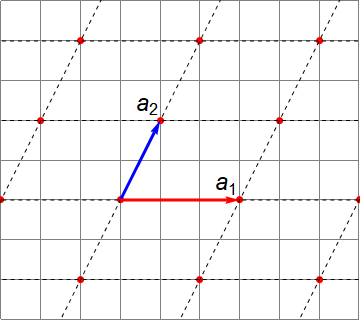
\includegraphics[width=0.40\textwidth]{HLBravaisLattice}
~~~
(b)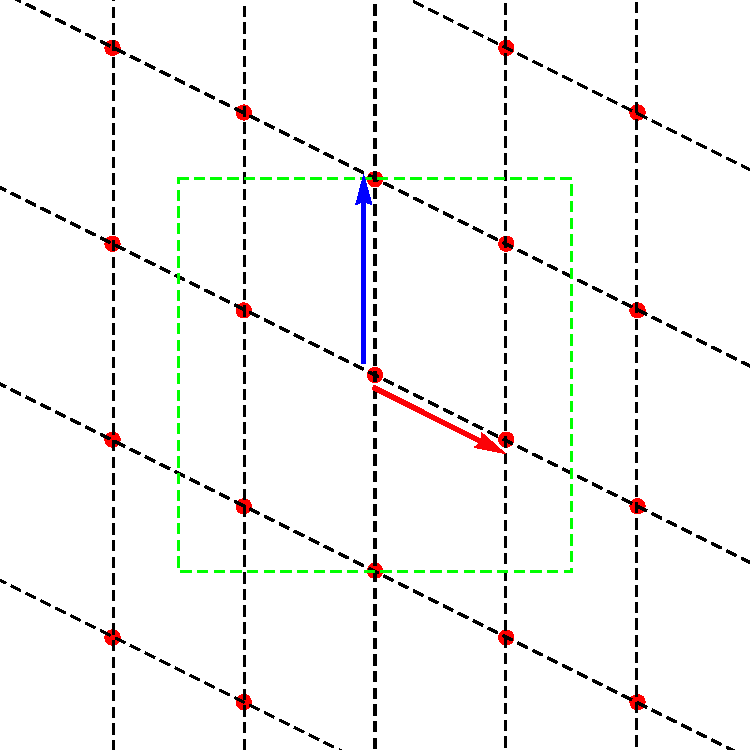
\includegraphics[width=0.40\textwidth]{HLReciprocalLattice1}
  \caption{\label{fig:HLReciprocalLattice}
%  (Color online)
(b)
    The reciprocal lattice \refeq{ReciprLattBasis}. Each reciprocal
    lattice point is a wave vector of the eigenvector of the translation
    operator with periodicity given by the Bravais lattice. The green
    dashed square encloses the first Brillouin zone of the {\em square
    lattice} (not the Bravais lattice). The wave vectors in the
    first Brillouin zone give all eigenvectors of the translation
    operator. Any wave vector outside of the first Brillouin zone is
    equivalent to a wave vector within it.
}
\end{figure}
%%%%%%%%%%%%%%%%%%%%%%%%%%%%%%%%%%%%%%%%%%%%%%%%%%%%%%%%%%%%%%%

    \PCpost {2019-09-11}{
Perhaps - if that helps:
copy to here the nomenclature used in \emph{PHYS-7143-19 week8}.
    }

    \PCpost{2019-11-24}{
    Do you have a closed form formula for counting these?
    We will need to include it in the paper. My
    $[2\!\times\!2]$ count
\(36 =
9+8+7+\cdots+1
\)
    was wrong.}

    \PCpost{2018-12-01}{ % 2020-01-11}{
Keep it as elementary as possible. Look at the beginning of the
\HREF{https://en.wikipedia.org/wiki/Chebyshev_polynomials} {wiki} - you can
already see our zeta function there. We need none of these funky trigonometric functions,
we only need the recurrence relations - they either already in this wiki, or in blogCats.tex,
or referred to in blogCats.tex.
    }

%\HLpost{2018-12-06}{
%I have a different way to prove \refeq{TableOfISP13952-2}. By the definition of the Chebyshev polynomials of the first kind:
%$\cos(n \theta) = T_n(\cos \theta)$, we can see that:
%\[
%T_\period{}\left[\cos\left(\frac{2 \pi j}{\period{}}\right)\right] = \cos(2\pi j) = 1 \, .
%\]
%So $\cos(2 \pi j /\period{})$, $j=0,1,...,\period{}-1$ are the roots of equation:
%\[
%T_n(x)-1=0 \, .
%\]
%So we have the identity:
%\beq
%T_n(x)-1 = 2^{\period{}-1} \prod_{j=0}^{\period{}-1} \left[x - \cos\left(\frac{2 \pi j }{\period{}}\right) \right]
%\, .
%\label{ProductToChebyshev}
%\eeq
%There is a coefficient $2^{\period{}-1}$ because the leading term in $T_n(x)$ is $2^{\period{}-1} x^\period{}$. Let $x=s/2$, and multiply both sides by 2, \refeq{ProductToChebyshev} becomes:
%\beq
%2T_n(s/2) - 2 = \prod_{j=0}^{\period{}-1} \left[s - 2\cos\left(\frac{2 \pi j }{\period{}}\right) \right]
%\, .
%\label{ProductToChebyshev-2}
%\eeq
%}

%%%%%%%%%%%%%%%%%%%%%%%%%%%%%%%%%%%%%%%%%%%%%%%%%%%%%%%%%%%%%
\begin{figure}
  \centering
(a)\includegraphics[width=0.45\textwidth]{HLLength2Counting}
(b)\includegraphics[width=0.45\textwidth]{HLLength3Counting-7210}
  \caption{\label{fig:HLCountingFigures}
(a) A 2-dimensional torus (with black border) stretched by $\jMorb$.
    The {\color{blue} blue} dots are internal integer points in the
    {\fundPip} (with red border). The {\color{green} green}
    dots are on the vertices of the {\fundPip}.
(b) A 3-dimensional torus (with black border) stretched by $\jMorb$.
    The {\color{blue} blue} dots are internal integer points in the
    stretched {\fundPip} (with red border). The {\color{green} green}
    dots are on the vertices of the {\fundPip}. The {
    pink} dots are on the surface of the {\fundPip}.
}
\end{figure}
%%%%%%%%%%%%%%%%%%%%%%%%%%%%%%%%%%%%%%%%%%%%%%%%%%%%%%%%%%%%%%%

%%%%%%%%%%%%%%%%%%%%%%%%%%%%%%%%%%%%%%%%%%%%%%%%%%%%%%%%%%%%%
% Predrag 2020-02-08 replaced Han's uneditable
% {HLLength2Counting}.pdf by catCyc2Jacob.svg
\begin{figure}
  \centering
(a)~\includegraphics[width=0.35\textwidth]{catCyc2Jacob}
~~~
(b)~\includegraphics[width=0.40\textwidth]{HLLength3Counting}
  \caption{\label{fig:catCycJacobOld}
Was \reffig{fig:catCycJacob}, now superannuated:
(a)
    $[2\!\times\!2]$ {\jacobianOrb} $\jMorb$ \refeq{catFundPar2}
    had a wrong sign, meaningless partition into 9 rectangles.
(b) Han 2020-02-11: Intermediate attempt to draw \reffig{fig:catCycJacob}.
$[3\!\times\!3]$ {\jacobianOrb} $\jMorb$  had tons of irrelevant points plotted,
    is unintelligible.
}
\end{figure}
%%%%%%%%%%%%%%%%%%%%%%%%%%%%%%%%%%%%%%%%%%%%%%%%%%%%%%%%%%%%%%%

    \PCpost{2020-0131}{
Maybe if you plot only the points within (inside, and on the 3 faces
connected to the origin) the {\fundPip} of
\reffig{fig:catCycJacob}, no other integer points, it might be easier
to understand. Also, if you trace out the cubic lattice in light gray, it
will be clear the periodic points are on the integer lattice, in the
spirit of \reffig{fig:BernCyc2Jacob}\,(b).
    }

    \PCpost{2020-02-08}{
To Han: not writing up what you are working on in the blog is
self-defeating, as I cannot help you as long as I am not aware of you
doing anything. However, not saving figure-generating code in
\emph{siminos/mathematica} is also inefficient, as you are making me
regenerate all figures from scratch.
    }

    \PCpost{2018-06-21}{
Your difficulty is that you keep on thinking in Hamiltonian way, where
one steps in time, using the Hamilton's equations for $(q_t,p_t)$, where
we had replaced the momentum $p_t$ (at spatial position $\ell$) by
velocity $p_t=(\ssp_{\ell t}-\ssp_{\ell,t-1})/\Delta t$, and thus
initializing the Hamiltonian, a second-order difference equation for
\emph{evolution in time} by two horizontal rows $(\ssp_{\ell
t},\ssp_{\ell,t-1})\,,\;\ell\in\integers$ in the spacetime plane.

You have to think in the spacetime, Lagrangian way instead. On each
lattice site $z=(\ell,t)$ there is a scalar field $\ssp_{\ell t}$, not a
two-torus. The field $\ssp_{\ell,t-1}$ belongs to a neighboring site
$z=(\ell,t-1)$. The two fields do not form a dynamical system on a
two-torus, as the dynamics is also influenced by spatial neighbors
$\ssp_{\ell\pm1, t}$.
    }

\PCpost{2017-09-16}{
%%%%%%%%%%%%%%%%%%%%%%%%%%%%%%%%%%%%%%%%%%%%%%%%%%%%%%%%%%%%%%%%%%%%%%%%
Methods described above make it an easy task to obtain a
particular class of \twots\ for  the {\catlatt}.

\twoT's
coordinate representation $\Gamma=\{\ssp_z, z\in \ZLT\}$, is obtained by
taking inverse of \refeq{2dCoupledCats}:
  \begin{equation}
   \ssp_z=\sum_{z'\in \ZLT} \gp_{zz'} \Ssym{z'}, \qquad    \Ssym{z'}\in \Ai,
  \end{equation}
where $\gp_{zz'}$ is the corresponding Green's function with periodic
{\bcs}.
%%%%%%%%%%%%%%%%%%%%%%%%%%%%%%%%%%%%%%%%%%%%%%%%%%%%%%%%%%%%%%%%%%%%%%%%
    } %end \PCpost

    \PCpost{2018-12-01}{
Include here the song and dance from the remark.
    \\
    What Hill's formula? Is it
    \refeq{MacMei83(17)}? Not any longer sure that
     \rf{MacMei83} contains the Hill's formula...


discrete Hill's formula\rf{BolTre10}:
\beq
\det(\jMps_\Mm - \matId) = \frac{(-1)^n \det \jMorb_\Mm}{\prod_{i=1}^n \det B_i}
\,,
\ee{BolTre10(2.8)a}
where for the one dimensional cat map the $B$ here is an $\BravCell{1}{1}{0}$ matrix:
\beq
B = - \frac{\delta^2 \genF[\ssp_{n+1},\ssp_{n}]}{\delta \ssp_{n+1} \delta \ssp_{n}} = 1
\,,
\ee{BolTre10(2.2)a}
    }


    \PCpost{2020-02-02}{
It is hard to find \refeq{LinearCatLatt} in {\GO}\rf{GutOsi15}. The paper
is mostly about the Hamiltonian formulation. Their (3.4) is the equation,
once on sets $c=d$ space-time isotropy, and drops their potential $V$.
Their perturbed equation (7.1) comes close to it. Their action (3.9) is a
bit mysterious as well.

Gutkin and Osipov\rf{GutOsi15}
refer to an \sPe\ \twot\ solution $p$ as a `many-particle periodic orbit', with
$\ssp_{n\zeit}$ `doubly-periodic', or `closed,'
\[
\ssp_{n\zeit} = \ssp_{n+\speriod{p},\zeit+\period{p}}
    \,,\quad
n = 0,1,2,\cdots, \speriod{p}-1
    \,;\quad
\zeit = 0,1,2,\cdots, \period{p}-1
    \,.
\]
    }

    \PCpost{2020-02-02}{
Note that in \refeq{catLatt} and throughout I have redefined the
stretching parameter ${s}$ to be stretching per dimension, \ie, ${s}$ in
\refeq{CatMap2d} is replaced by $d{s}$. This is consistent with
how one defines a diffusion constant on an isotropic $d$\dmn\ hypercubic
lattice.
    }

	\PCpost{2019-08-06}{% Is the lattice cell called the primitive cell?
    I do not think ``lattice cell'' is the standard terminology, and as
    you have chosen not to quotient the point group, what you have is not
    `primitive' - that would be 1/8th triangle that tiles the first
    Brillouin zone, I think. Please strictly follow the nomenclature of a
    single reference -presumably Dresselhaus \etal\rf{Dresselhaus07}, or
    Barvinok\rf{Barvinok08} or whatever  - and state so clearly in your
    text. Whenever you use a reference, ethics of the profession requires
    that you clearly cite it.
       }

    \PCpost{2020-01-27}{{\bf to Han -}
For us there is no field $\Xx({z})$ defined over continuum space
$z\in\reals^d$, only $\ssp_z$. Our problems live on the integer lattices
$z\in\integers^d$. This might be called `tight-binding models'. Please
verify whether that's what `tight-binding models' are.
    }

    \HLpost{2020-02-20}{
\refFig{fig:HLfundPip2by1_1} is the \fundPip\ of a $[2\!\times\!1]_1$
\twot. The pattern of this periodic state is shown in \reffig{fig:2x1rpo}
(a). The \jacobianOrb\ of this \twot\ can be written as a
$[2\!\times\!2]$ matrix:
\[
    \jMorb
    =
     \left(\begin{array}{cc}
 -2s &  4 \\
  4 & -2s
 \end{array} \right) \, .
    \]
The shape of the \fundPip\ is very similar to \reffig{fig:catCycJacob} (a).
    }
%%%%%%%%%%%%%%%%%%%%%%%%%%%%%%%%%%%%%%%%%%%%%%%%%%%%%%%%%%%%%%%%%%
%\FIG{
\begin{figure}
  \centering
\includegraphics[width=0.40\textwidth]{HLfundPip2by1_1}
  \caption{\label{fig:HLfundPip2by1_1}
The \fundPip\ of a $[2\!\times\!1]_1$ \twot\ with $s=5/2$. Admissible field values lie within the unit square with blue boundaries. This unit square is stretched by the \jacobianOrb\ $\jMorb$ into the \fundPip\ with red boundaries. Integer points in the \fundPip\ are marked by the circles. There are 9 integer points in the \fundPip, in agreement with the counting formula.
            }
\end{figure}
%%%%%%%%%%%%%%%%%%%%%%%%%%%%%%%%%%%%%%%%%%%%%%%%%%%%%%%%%%%%%%%%%%

    \PCpost{2018-12-13}{
Must rethink the DIMENSION of $F[\Xx]$ and $\jMorb$. $F[\Xx]_i$
is a $\cl{}$\dmn\ vector function - is it dimensionally the same as
$\ssp_j$? Otherwise \jacobianOrb\ is not dimensionless, and cannot be
referred to as a `Jacobian'. Relation \refeq{detDet} only makes sense for
the dimensionless case. I think we are OK, but we have to be sure.
    }

%%%%%%%%%%%%%%%%%%%%%%%%%%%%%%%%%%%%%%%%%%%%%%%%%%%%%%%%%%%%%%%%%%%%%%%
% BernCyc2Jacob.svg
% derived from CatMapStatesp.svg
\begin{figure}
  \centering
{(a)}
\includegraphics[width=0.35\textwidth]{BernCyc2Jacob}
~~~
{(b)} %$\!\!\!\!$
\includegraphics[width=0.35\textwidth]{BernCyc2JacobUnit}
  \caption{\label{fig:BernCyc2JacobOld}
[OLD VERSION] The Bernoulli map \refeq{BerShift} period-2 lattice states
$\Xx_\Mm=(\ssp_0,\ssp_1)$ are the $\cycle{0}=(0,0)$ fixed
point, and the 2-cycle $\Xx_{01}=({1}/{3},{2}/{3})$, see
\reffig{fig:BernPart}\,(a). They all lie within the unit square $[0BCD]$,
one within each $\pS_{\Ssym{0}\Ssym{1}}$ subregion, and are mapped by the
$[2\!\times\!2]$ {\jacobianOrb} $\jMorb$ \refeq{bernFundPar} into the
{\fundPip} $[0B'C'D']$. The images
of periodic points $\Xx_\Mm$ land on the integer lattice, and are sent back
into the origin by integer translations $\Mm$, in order to satisfy the
fixed point condition \refeq{tempFixPoint}, $\jMorb\Xx_\Mm+\Mm=0$.
\refFig{fig:BernPart}\,(a) suggests subdividing the {\fundPip}
into (a) 4 areas, but they are not unit areas. The theory of integer lattices
dictates instead (b) covering the {\fundPip} by 3 unit area
rectangles, with
all vertices on the integer lattice.
          }
\end{figure}
%%%%%%%%%%%%%%%%%%%%%%%%%%%%%%%%%%%%%%%%%%%%%%%%%%%%%%%%%%%%%%
%


    \PCpost{2019-08-11}{
to Han: this is wrong alphabet, for the
symmetric unit interval $\ssp\in[-1/2,1/2)$.
For all our examples we pick
the `least stretching' \catlatt\ with $s=5/2$,
with 9-letter alphabet
\beq
\A=\{\underline{4},\underline{3},\underline{2},\underline{1},
     0,1,2,3,4\}
\,.
\ee{catLattAlphabet}
    }

    \PCpost{2020-02-17}{
Now in \reftab{tab:LxTs}:
\bea
N_{\BravCell{1}{1}{0}}({s}) = 2({s}-2)
    \continue
N_{[2\!\times\!1]}({s}) = 4({s}-2)s
    \continue
N_{[2\!\times\!1]_1}({s}) = 4({s}-2)({s}+2)
    \continue
N_{[2\!\times\!2]}({s}) = 16({s}-2)s^2({s}+2)
    \continue
N_{\BravCell{3}{2}{0}}({s}) = 4({s}-2)s(2{s}-1)^2 (2{s}+3)^2
    \continue
N_{\BravCell{3}{2}{1}}({s}) = 64({s}-2){s}^3 ({s}+1)^2
    \continue
N_{\BravCell{3}{2}{2}}({s}) = 64({s}-2){s}^3 ({s}+1)^2
    \continue
N_{[3\!\times\!3]}({s}) = -32({s}-2)({s}+1)^4(2{s}-1)^4
\,.
\label{PC[LxT]volume}
\eea
    }

    \PCpost{2019-11-23}{Dropped:
For all our examples we pick
the `least stretching' hyperbolic \catlatt\ with $s=5$,
and restrict the
admissible field values $\ssp_{z}$ at lattice site $z=(n_1,n_2)$ to the
symmetric unit interval $\ssp\in[-1/2,1/2)$, with 9-letter alphabet
\refeq{catLattAlphabet}

the code depends on the choice of the unit interval:
the alphabet \A\ for $\ssp_{\zeit} \in [-1/2,1/2)$
differs from the alphabet for  $\ssp_{\zeit} \in [0,1)$.

Here $s=5/2$ and $\ssp_z\in[-1/2,1/2)$, so the
interior alphabet is one letter alphabet $\Ai=\{0\}$...

    }

    \PCpost{2020-02-24}{
Thanks for fixing \reftab{tab:LxTs=5/2} and \reftab{tab:LxTs}. Apparently
I am not evaluating \emph{Tensors.nb} correctly - you'll show me how.
    }

    \PCpost{2020-02-23}{
Just curious - what does the Bernoulli {\fundPip} defined by the columns
of $[3\!\times\!3]$ {\jacobianOrb}
\beq
\jMorb =
\left(
\begin{array}{ccc}
  1 & -2 &  0 \\
  0 &  1 & -2 \\
  -2&  0 &  1
\end{array}
\right)
\,,
\qquad
N_3 = |\Det \jMorb|
    = 2^3-1
\,,
\label{bernFundPar3}
\eeq
look like in a 3\dmn\ rendition? Hopefully it is not symmetric, like
\reffig{fig:catCycJacob}\,(b).
    }

    \PCpost{2020-02-08}{
I think the $N_\cl{}=({s}-2)\cdots$ factorization is true for all $\cl{}$
in \refeq{1stChebGenF} and \reftab{tab:LxTs}. Do you understand it? Does
in the \templatt\ $s=2$ case, the Laplacian has a zero mode? A constant
$\ssp_i$ eigenvector? If so, why doesn't the \catlatt\ have
$N=({s}-2)^2\cdots$, one for each direction? Instead, one gets only a factor 2,
$N=2({s}-2)\cdots$.
    }

%    \PCpost{2020-02-24}{
%I had naively thought that $N_{\BravCell{\speriod{}}{1}{0}}$ families were
%the same as the 1\dmn\ \templatt\ \refeq{1stChebGenF}. Apparently not. Do
%you see something like a Chebyshev series here, or generating function
%similar to \refeq{Isola90-13}? If we cannot figure the bivariate zeta
%function, at least this family should work out?
%    }

    \PCpost{2020-02-24}{
Not urgent, but can you complete the primitive counts
$M_{[\speriod{}\!\times\!\period{}]_S}$ and decompositions of
$N_{[\speriod{}\!\times\!\period{}]_S}$ into primitive \twots\ in
\reftab{tab:LxTs=5/2} and perhaps also in \reftab{tab:LxTs}?
    }


    \PCpost{2020-03-05}{\tempLatt\ counting (all messed up,
    fix using \\ \emph{CatMaptopZeta.nb} output):
\bea
\sum_{{n}=0}^\infty N_{n} z^{n}
    & = & \frac{2-{s}z}{1 - s z + z^2}-\frac{2}{1 - z}
    \continue
\{N_{n}\} & = & s-2,s^2-4,
       s^3-3s-2,
        s^4-4s^2,
    \ceq
        2 \left(s^5-4 s^3+3 s\right)-s \left(s^4-3 s^2+1\right)-2,
    \ceq
        -2 \left(s^3-2s\right)-s\left(s^4-3 s^2+1\right)
    \ceq
-2 - s (-1 + 6 s^2 - 5 s^4 + s^6) + 2 (-4 s + 10 s^3 - 6 s^5 + s^7),
    \ceq
        -2s \left(s^5-4 s^3+3 s\right)-2 \left(s^4-3s^2+1\right)-2,
    \ceq
        -2 \left(s^5-4 s^3+3 s\right)
        +s \left(s^6-5 s^4+6s^2-1\right)-2,
        %s \left(s^7-6 s^5+10 s^3-4 s\right)-2 \left(s^6-5 s^4+6
%s^2-1\right)-2,-2 \left(s^7-6 s^5+10 s^3-4 s\right)+s \left(s^8-7 s^6+15
%s^4-10 s^2+1\right)-2,s \left(s^9-8 s^7+21 s^5-20 s^3+5 s\right)-2
%\left(s^8-7 s^6+15 s^4-10 s^2+1\right)-2,-2 \left(s^9-8 s^7+21 s^5-20
%s^3+5 s\right)+s \left(s^{10}-9 s^8+28 s^6-35 s^4+15 s^2-1\right)-2,s
%\left(s^{11}-10 s^9+36 s^7-56 s^5+35 s^3-6 s\right)-2 \left(s^{10}-9
%s^8+28 s^6-35 s^4+15 s^2-1\right)-2
\,,
\label{1stChebGenFdrop}
\eea
    }

     \PCpost{2020-03-23} {
Lot's of headless \KSe\ floundering in preparing \emph{BlogCats.tex}
\refsect{sect:KSe} saved below. Hopefully the resulting discretized \KSe\
\refeq{KSdiscr5} is correct...

\medskip

The discretized \KSe\ is of the form
\beq
\pde_\zeit \mathsf{U} + \frac{\alpha}{2}\pde_x\mathsf{U}^2
  - \beta\,\Laplacian_x \mathsf{U} + \gamma\,\Laplacian_x^2 \mathsf{U}
= 0
\,.
\ee{KSdiscr1}
Rescale $\mathsf{U}\to\mathsf{U}/\Delta\zeit$
%, divide by $\Delta x$:
\beq
\frac{\pde_\zeit}{\Delta\zeit}\mathsf{U}
+ \frac{(\Delta x)^2}{\Delta\zeit}\frac{\alpha}{2}\frac{\pde_x}{\Delta x}\mathsf{U}^2
  - \frac{(\Delta x)^2}{\Delta\zeit}\beta\,\frac{\Laplacian_x}{(\Delta x)^2} \mathsf{U}
  + \frac{(\Delta x)^4}{\Delta\zeit}\gamma\,\frac{\Laplacian_x^2}{(\Delta x)^4}\mathsf{U}
= 0
\,.
\ee{KSdiscr2}
Our canonical choice is setting these
\beq
\alpha=\frac{\Delta\zeit}{(\Delta x)^2}
    \,,\quad
\beta=-\frac{\Delta\zeit}{(\Delta x)^2}
    \,,\quad
\gamma=\frac{\Delta\zeit}{(\Delta x)^4}
\,,
\ee{KSscales}
equal to 1, parametrazing the problem with
$\speriod{}=1/\Delta x$, $\period{}=1/\Delta\zeit$,
\beq
\frac{1}{\period{}}\frac{\pde_\zeit}{\Delta\zeit} \mathsf{U}
  + \frac{1}{\speriod{}}\frac{\alpha}{2}\frac{\pde_x}{\Delta x}\mathsf{U}^2
  - \frac{1}{\speriod{}^2}\beta\,\frac{\Laplacian_x}{(\Delta x)^2} \mathsf{U}
  + \frac{1}{\speriod{}^4}\gamma\,\frac{\Laplacian_x^2}{(\Delta x)^4}\mathsf{U}
= 0
\,.
\ee{KSdiscr3}
Rescale $\mathsf{U}\to\mathsf{U}\,\period{}$
\beq
\frac{\pde_\zeit}{\Delta\zeit} \mathsf{U}
  + \frac{\period{}^2}{\speriod{}}\frac{\alpha}{2}\frac{\pde_x}{\Delta x}\mathsf{U}^2
  - \frac{\period{}}{\speriod{}^2}\beta\,\frac{\Laplacian_x}{(\Delta x)^2} \mathsf{U}
  + \frac{\period{}}{\speriod{}^4}\gamma\,\frac{\Laplacian_x^2}{(\Delta x)^4}\mathsf{U}
= 0
\,.
\ee{KSdiscr4}
Our canonical choice is setting these
\beq
\alpha=\speriod{}/\period{}^2
    \,,\quad
\beta=-\speriod{}^2/\period{}
    \,,\quad
\gamma=\speriod{}^4/\period{}
\,,
\ee{KSscales1}
equal to 1,
\beq
\frac{\pde_\zeit}{\Delta\zeit} \mathsf{U}
  + \frac{1}{2}\frac{\pde_x}{\Delta x}\mathsf{U}^2
  + \frac{\Laplacian_x}{(\Delta x)^2} \mathsf{U}
  + \left(\frac{\Laplacian_x}{(\Delta x)^2}\right)^2\mathsf{U}
= 0
\,,
\ee{KSdiscr4}
    }

%    \PCpost{2020-02-24}{
% Priority \# 1: {\em appeFourier.tex}.
%    }

    \PCpost{2019-12-28}{
My argument along the following lines was unnecessarily complicated:
%where we have used
\beq
%\sum_{k=0}^{\cl{}-1} \epsilon^{k} = 0 \,,\qquad
\epsilon^0\epsilon^1\epsilon^2\cdots\epsilon^{\cl{}\!-\!1}=1
\,.
\ee{circKron}
can be eliminated by going from products
to sums over cyclic eigenvalues. For example, if
a polynomial is of form
\(
G(x)/(x-\lambda_0)
\,,
\)
with the zeroth root
\(
(x-\epsilon^0)= (x-1)
\)
quotiented out from the characteristic polynomial, % \refeq{CNcharPoly},
\[
\frac{x^N-1}{x-1}
=
(x-\epsilon)(x-\epsilon^2)\cdots(x-\epsilon^{N-1})
\,.
\]
Consider a sum of the first $N$ terms of a geometric series,
multiplied by $(x-1)/(x-1)$:
\beq
1+x+\cdots + x^{N-1}
=
\sum_{m=0}^{N-1} x^m
=
\frac{1}{x-1} \sum_{m=0}^{N-1} (x-1)\,x^m
=
\frac{x^N-1}{x-1}
\,.
\ee{BG:PartSum}
So, the products can be written as sums
\beq
(x-\epsilon)(x-\epsilon^2)\cdots(x-\epsilon^{N-1})
=
1+x+\cdots + x^{N-1}
\,.
\ee{BG:PartSum1}
In \Cn{N} $P_n$ projection operators, the denominators are
evaluated by substituting $x\to1$ into \refeq{BG:PartSum1}; that adds up
to $N$.
The numerator is evaluated by substituting $x\to\epsilon^{-n} M$.
We obtain the projection operator as a discrete Fourier weighted sum
of matrices $M^m$,
\beq
P_n=\frac{1}{N}\sum_{m=0}^{N-1}e^{-i\,\frac{2\pi}{N}nm}\,M^m
\,,
\ee{examDisFourT}
instead of the usual product form.
    }

    \PCpost{2020-06-02}{dropped:
A given \brick\ $\Mm$ is \emph{\admissible} if the corresponding lattice
state $\Xx$ satisfies the temporal Bernoulli \refeq{1stepDiffEq}
condition \(\ssp_{\zeit} \in [0,1)\) at {every lattice site}
$\zeit\in\integers$.
In case at hand, all itineraries are allowed, except for the rightmost
fixed point
\(
\{\Ssym{\zeit}\}=s-1
\,,
\)
which is identified with
\(
\{\Ssym{\zeit}\}=0
\,,
\)
see \reffig{fig:BernPart}.
    }

    \PCpost{2020-06-08}{dropped:
The periodicity of the periodic lattice states are described by the $d$\dmn\ Bravais lattice:
\beq
\Lambda =
\left\{ \sum_{i=1}^d n_i \mathbf{a}_i\,|\,n_i \in \mathbb{Z}\right\} \, .
\ee{dDBravaisLattice}

The {\jacobianOrb} \refeq{catlattFix} is constructed from $d$ commuting
translation operators $\hopMat_{i}$ with $i=1, \dots, d$. The eigenvectors of these translation
operators are plane waves:
 \beq
f_{k}({z}) = e^{i {k} \cdot {z}}
\,,
\ee{PlaneWave}
where $\mathbf{k}$ is a $d$\dmn\ wave vector. A general plane wave does not
satisfy the periodicity \refeq{dDPeriodicCondition}, unless
\beq
e^{i {k} \cdot {R}} = 1
\, .
\ee{PeriodicPlaneWave}
Since ${R}$ is a vector from the Bravais lattice $\Lambda$, the wave
vector $\mathbf{k}$ must lie in the reciprocal lattice of $\Lambda$:
\beq
\mathbf{k} \in \Lambda^*
\,,\quad
\Lambda^* =
\left\{ \sum_{i=1}^d m_i \mathbf{b}_i\,|\,m_i \in \mathbb{Z}\right\} \, ,
\ee{dDReciprocalLattice}
where the primitive reciprocal lattice vectors $\mathbf{b}_i$ satisfy:
 \beq
\mathbf{b}_i \cdot \mathbf{a}_j = 2 \pi \delta_{ij} \, .
\ee{ReciprLattBasis}
To get the eigenvectors and the corresponding eigenvalues
of the \jacobianOrb, note that
\beq
(\hopMat_j + \hopMat_{j}^{-1}) e^{i {k} \cdot {z}}
=
e^{i ({k} \cdot {z} - k_j)} + e^{i ({k} \cdot {z} + k_j)}
=
(2 \cos k_j) e^{i {k} \cdot {z}} \, ,
\ee{EigenvalueTranslation}
where the $\mathbf{k}=(k_1,k_2,\cdots,k_d)$. Hence the eigenvalue of the
{\jacobianOrb} \refeq{catlattFix} corresponding to the eigenvector with
the wave vector $\mathbf{k}$ \refeq{PlaneWave} is
\beq
\lambda_{k} = \sum_{j=1}^d \left( 2\cos k_j - s \right)
\,.
\ee{dDEigenvalue}

, and compute
its inverse, the Green's function.
\bigskip

The generalization to $d$ \spt\ dimensions is immediate.
A periodic {lattice state} ${\Xx}=\{\ssp_z\}$, $z\in\integers^d$ is
a {point} within the $(\ell_1\ell_2\cdots\ell_d)$\dmn\
unit hyper-cube $[0,1)^{\ell_1\ell_2\cdots\ell_d}$, where $\ell_j$
is the lattice period in direction $j$, and the
$(\ell_1\ell_2\cdots\ell_d)^2$\dmn\ {\jacobianOrb} $\jMorb_{zz'}$ is
given by
\beq
\jMorb = \sum_{j=1}^{d}\left(\hopMat_j-{s}\unit+\hopMat_{j}^{-1}\right)
\,.
\ee{catlattFixover}
Here $\hopMat_i$ is a {\shiftOp}
\refeq{hopMatrix} which translates the field in the $i$th
direction by one lattice spacing. Its inverse $\hopMat_{i}^{-1}$
translates the field in the negative $i$th direction.


From now on we specialize to the 2\dmn, $z=(n,\zeit)\in\integers^2$
\spt\ lattice, and replace the $(\ell_1,\ell_2)$ notation for lattice
periods by $(\speriod{},\period{})$, where $\speriod{}$ is the `spatial',
and $\period{}$ the `temporal' lattice period. The field $\ssp_i$
takes values in the $\speriod{}\period{}$\dmn\ unit hyper-cube
$\Xx\in[0,1)^{\speriod{}\period{}}$.

Throw away all {\brick}s which are repeats of
shorter {\brick}s in the temporal direction. What
remains in $N_k$ prime periodic \brick s $p$ of the same size
$[\speriod{p}\times\period{p}]=[\speriod{k}\times\period{k}]$.

This is essential to all that follows, as the Lagrangian formulation will
apply to \catlatt\ in any number of spatial dimensions as well.

  }

\PCpost{2020-05-31} {
  {\em Periodic
orbits in coupled {H{\'e}non} maps: {Lyapunov} and multifractal analysis}
is quite close to our \catlatt. The problem is harder,
as the {H{\'e}non} map is nonlinear.
    }



    \PCpost{2020-05-28}{
    Track this down:
Vicky Weiskopf: ``It is better to uncover a little than cover a lot''
    }
\end{description}


\subsection{Hill's formula:
             stability of an orbit vs. its time-evolution stability}

{\bf 2020-07-14 Han}

To prove the Hill's formula \refeq{detDetCat} for the cat map, first note that both the left hand side and right hand side are polynomials with the same leading terms $s^\cl{}$. The left hand side is the determinant of the tri-diagonal Toeplitz matrix \refeq{Hessian}.  From the \refeq{StabMtlpr} and \refeq{noPerPts}, the right hand side can be written in the form
\bea
|\det(\jMps^{\cl{}} - \matId)|
          &=& \ExpaEig^{\cl{}} + \ExpaEig^{-\cl{}} - 2 \continue
          &=& 2 \cosh( \cl{} \Lyap) -2 \continue
          &=& 2 \cosh \left[ \cl{} \textrm{arc}\cosh\left(\frac{s}{2}\right)\right] -2
          \,,
\label{HillsForRight}
\eea
where we used $s=2\cosh(\Lyap)$. Known that the Chebyshev polynomial of the first kind can be written as $T_\cl{}(x) = \cosh [ \cl{} \textrm{arc}\cosh(x)]$, the right hand side of \refeq{detDetCat} is
\[
|\det(\jMps^{\cl{}} - \matId)|
=
2 T_\cl{}\left(\frac{s}{2}\right)-2 \, ,
\]
which has the leading term $s^\cl{}$.

Let $u = (u_j)_{j = 1, 2, \dots, \cl{}}$ be the variation to the periodic orbit $\Xx$ with length $\cl{}$. $\jMorb u = 0$ only if $\jMps^\cl{} w = w$ where $w=(u_1,u_2)$. Then $|\det(\jMps^{\cl{}} - \matId)|=0$ is equivalent to $|\det(\jMorb)|=0$. Then the polynomials $|\det(\jMorb)|$ and $|\det(\jMps^{\cl{}} - \matId)|$ have the same roots and the same leading terms so they are equal.

{\bf 2020-07-17 Han}

Let $s$ go to infinity. Then the stability multipliers becomes:
\bea
\lim_{s \to \infty} \ExpaEig = \lim_{s \to \infty} \frac{s+\sqrt{s^2-4}}{2} = s \, , \continue
\lim_{s \to \infty} \ExpaEig^{-1} = \lim_{s \to \infty} \frac{2}{s+\sqrt{s^2-4}} = \lim_{s \to \infty} \frac{1}{s} =0 \, .
\label{StabMtlprLimit}
\eea
Then in the limit:
\beq
\lim_{s \to \infty} |\det(\jMps^{\cl{}} - \matId)|
          = \lim_{s \to \infty} \ExpaEig^{\cl{}} + \ExpaEig^{-\cl{}} - 2
          = s^\cl{}
          \,,
\ee{HillsForRightLimit}
So the leading term of the right hand side of \refeq{detDetCat} is $s^\cl{}$.

\bea
|\det(\jMps^{\cl{}} - \matId)|
          &=& \ExpaEig^{\cl{}} + \ExpaEig^{-\cl{}} - 2 \continue
          &=& \left(\frac{s+\sqrt{s^2-4}}{2}\right)^\cl{} + \left(\frac{s-\sqrt{s^2-4}}{2}\right)^\cl{} -2 \continue
          &=& \frac{1}{2^\cl{}} \sum_{k=0}^{\frac{\cl{}}{2}} {2k \choose \cl{}} s^{\cl{}-2k}(s^2-4)^k - 2
          \,,
\label{HillsForRight}
\eea

{\bf 2020-07-21 Han}
The \jacobianOrb\ of the \templatt\ has form:
\[
\jMorb
=
\left(
\begin{array}{cccc}
 -s & 1 & 0 & 1 \\
 1 & -s & 1 & 0 \\
 0 & 1 & -s & 1 \\
 1 & 0 & 1 & -s \\
\end{array}
\right)
\, ,
\]
while the \jacobianOrb\ from \refeq{bernNotHill} is
\[
\jMorb'=\unit- \hopMat^{-1} \otimes \jMps
=
\left(
\begin{array}{cc|cc|cc|cc}
 1 & 0 & 0 & 0 & 0 & 0 & 0 & -1 \\
 0 & 1 & 0 & 0 & 0 & 0 & 1 & -s \\ \hline
 0 & -1 & 1 & 0 & 0 & 0 & 0 & 0 \\
 1 & -s & 0 & 1 & 0 & 0 & 0 & 0 \\ \hline
 0 & 0 & 0 & -1 & 1 & 0 & 0 & 0 \\
 0 & 0 & 1 & -s & 0 & 1 & 0 & 0 \\ \hline
 0 & 0 & 0 & 0 & 0 & -1 & 1 & 0 \\
 0 & 0 & 0 & 0 & 1 & -s & 0 & 1 \\
\end{array}
\right)
\, .
\]
We know that
\[
\det \left( \unit- \hopMat^{-1} \otimes \jMps \right)
=
\det \left( \unit-\jMps \otimes \hopMat^{-1} \right)
=
\det \left[\left( \unit-\jMps \otimes \hopMat^{-1} \right) \left( \unit_{[2\times 2]} \otimes \hopMat \right)\right]
\, ,
\]
where
\[
\unit-\jMps \otimes \hopMat^{-1}
=
\left(
\begin{array}{cccc|cccc}
 1 & 0 & 0 & 0 & 0 & 0 & 0 & -1 \\
 0 & 1 & 0 & 0 & -1 & 0 & 0 & 0 \\
 0 & 0 & 1 & 0 & 0 & -1 & 0 & 0 \\
 0 & 0 & 0 & 1 & 0 & 0 & -1 & 0 \\ \hline
 0 & 0 & 0 & 1 & 1 & 0 & 0 & -s \\
 1 & 0 & 0 & 0 & -s & 1 & 0 & 0 \\
 0 & 1 & 0 & 0 & 0 & -s & 1 & 0 \\
 0 & 0 & 1 & 0 & 0 & 0 & -s & 1 \\
\end{array}
\right)
\, ,
\]
and
\[
\left( \unit-\jMps \otimes \hopMat^{-1} \right) \left( \unit_{[2\times 2]} \otimes \hopMat \right)
=
\left(
\begin{array}{cccc|cccc}
 0 & 1 & 0 & 0 & -1 & 0 & 0 & 0 \\
 0 & 0 & 1 & 0 & 0 & -1 & 0 & 0 \\
 0 & 0 & 0 & 1 & 0 & 0 & -1 & 0 \\
 1 & 0 & 0 & 0 & 0 & 0 & 0 & -1 \\ \hline
 1 & 0 & 0 & 0 & -s & 1 & 0 & 0 \\
 0 & 1 & 0 & 0 & 0 & -s & 1 & 0 \\
 0 & 0 & 1 & 0 & 0 & 0 & -s & 1 \\
 0 & 0 & 0 & 1 & 1 & 0 & 0 & -s \\
\end{array}
\right)
\,.
\]
The determinant of a block matrix is
\[
\det
\left(
\begin{array}{cc}
A & B \\
C & D \\
\end{array}
\right)
=
\det(A)\det(D-CA^{-1}B)
\, .
\]
Then we have:
\[
\det \left[\left( \unit-\jMps \otimes \hopMat^{-1} \right) \left( \unit_{[2\times 2]} \otimes \hopMat \right)\right]
=
\det [-s \unit + \hopMat - \unit \hopMat^{-1} (-\unit)]
=
\det \jMorb
\,.
\]


What happens if we change the order of how we block the matrix, and
consider ${\mathbf{\jMps}_1} \otimes \hopMat_2^{-1}$ instead of
$\hopMat_2^{-1}\otimes{\mathbf{\jMps}_1}$ in \refeq{eq:orbitJPVtempJ}?

In particular, by similarity relation \refeq{wikiKron3},
\refeq{eq:orbitJPVtempJ} is equivalent to ...

\begin{description}
    \PCpost{2020-07-25} {
%\subsection{\catLatt\ Hill's formula leftovers}
%\label{sect:catlattHillover}
%Not used in {\em CL18}:




\bigskip\bigskip



using
\beq
\det
\left(
\begin{array}{cc}
A & B \\
C & D \\
\end{array}
\right)
=
\det(D)\,\det(A-BD^{-1}C)
\,.
\ee{det2x2blockMat1}
so (not rechecked),
\bea
\det(1-\mathbf{\jMps} \otimes \hopMat^{-1})
    &=&
\det
 \left[\begin{array}{cc}
\unit_1 & -\unit_1\\
\unit_1 & {\unit_1+\mathbf{\jMorb}_1}
\end{array}
\right]
=
\det({2\unit_1+\mathbf{\jMorb}_1})\,\det(\unit_1)
%\det [- 2(s-1)\unit + \hopMat - \unit \hopMat^{-1} (-\unit)] =
    \continue
    &=&
\det [\hopMat - 2(s-1)\unit + \hopMat^{-1}]
    =
|\det \jMorb |
\,.
\label{det2x2blockMat2}
\eea

in time with a [$2\speriod{}\!\times\!2\speriod{}$] block matrix
$\hat{\mathbf{\jMps}}$,
    \PC{2020-07-15}{
    Rewriting here \refeq{HLpartition2d}, \refeq{HLpartition2d2} as
    \refeq{CatMap2dHill}; will use $\mathsf{U}$ for the variation of \Xx.
    }
\bea
\hat{\Xx}_{\zeit+1} &=&
  \hat{\mathbf{\jMps}} \hat{\Xx}_\zeit - \hat{\mathsf{\Ssym{}}}_\zeit
\,,\qquad %\continue
\hat{\mathbf{\jMps}}  =
 \left[\begin{array}{cc}
{\bf 0} & {\bf I}\\
{\bf -I} & {-{\bf \jMorb}_\zeit}
 \end{array} \right]
 \,.
\label{HLpartition2d_Hill}
\eea

The \HREF{https://en.wikipedia.org/wiki/Kronecker_product} {Kronecker
product} $\mathbf{A}\otimes\mathbf{B}$ is an operation by [$m\times n$]
matrix $\mathbf{A}$ on [$p\times q$] matrix $\mathbf{B}$, resulting in an
[$pm\times qn$] block matrix:
\beq
\mathbf{A}\otimes\mathbf{B} =
\left(\begin{array}{ccc} %\begin{bmatrix}
  a_{11} \mathbf{B} & \cdots & a_{1n}\mathbf{B} \\
             \vdots & \ddots &           \vdots \\
  a_{m1} \mathbf{B} & \cdots & a_{mn} \mathbf{B}
\end{array}\right) %\end{bmatrix}
\,,
\ee{KroneckerProdover}

\beq
\tr(\mathbf {A} \otimes \mathbf {B} )
=\tr\mathbf {A} \,\tr\mathbf {B} \quad\mbox{and}\quad \det(\mathbf {A} \otimes \mathbf {B} )=(\det \mathbf {A} )^{m}(\det \mathbf {B} )^{n}
\,.
\ee{wikiKron2over}

$\mathbf{\jMorb}_1$ is the spatial $[\speriod{}\!\times\!\speriod{}]$
{\jacobianOrb} of  form (XX),
\bea
\mathbf{\jMorb}_1
        &=&
\hopMat_{1}^{-1} - 2s \unit_1 + \hopMat_{1}
        \continue
        &=&
\left(\begin{array}{cccccc}
 -{2s}& 1 & 0 & \dots   & 1 \\
 1 &  -{2s}& 1 & \dots  & 0 \\
\vdots & \vdots &\vdots &\ddots &\vdots\\
 1 & 0 & \dots & 1      & -{2s}
        \end{array} \right)
\,.
\label{Hessian_Hillover}
\eea

If $\mathbf{A}$, $\mathbf{B}$, $\mathbf{C}$ and $\mathbf{D}$ are matrices
of such size that one can form the matrix products $\mathbf{AC}$ and
$\mathbf{BD}$, then the product of two block matrices is
a block matrix:
\beq
(\mathbf{A}\otimes\mathbf{B})\,(\mathbf{C}\otimes\mathbf{D})
%= (\mathbf{A}\mathbf{C})\otimes(\mathbf{B}\mathbf{D})
%  {\displaystyle (\mathbf {A} \otimes \mathbf {B} )(\mathbf {C} \otimes \mathbf {D} )
  =(\mathbf{AC})\otimes (\mathbf{BD})
  \,.
\ee{mixedProdover}

If $\lambda _{1}, ..., \lambda _{n}$ are the eigenvalues of $\mathbf{A}$,
and $\mu_{1}, ..., \mu_{m}$ the eigenvalues of $\mathbf{B}$, then the
eigenvalues of $\mathbf{A}\otimes\mathbf{B}$ are
\beq
\lambda_{i}\mu_{j},\qquad i=1,\ldots ,n,\,j=1,\ldots ,m
\,,
\ee{wikiKron1}

temporal {\jacobian} matrix %$\mathbf{\jMps}$
\beq
 \mathbf{\jMps}
=
 \left(\begin{array}{cc}
 0 & 1 \\
 -1 & s
 \end{array} \right)
% +
% \left(\begin{array}{cc}
% 0 & 0 \\
% 0 & s
% \end{array} \right)
 =
 \omega
    \left(
 \unit
 -
 \omega
 \left(\begin{array}{cc}
 0 & 0 \\
 0 & s
 \end{array} \right)
    \right)
\,.
\ee{eq:StateSpCatMap_Hillover}

\bea
\hat{\Xx}_{\zeit+1} &=&
  \jMps_{PV} \hat{\Xx}_\zeit - \hat{\mathsf{\Ssym{}}}_\zeit
    \continue
\jMps_{PV} &=&
 \left[\begin{array}{cc}
{\bf 0} & {\bf I}\\
{\bf -I} & {-{\bf \jMorb}_\zeit}
 \end{array} \right]
            =
{\omega} -
 \left[\begin{array}{cc}
{\bf 0} & {\bf 0}\\
{\bf 0} & {{\bf \jMorb}_\zeit}
 \end{array} \right]
\label{HLpartition2d_Hillover}
\eea
 as
a generalization of the $\speriod{}=1$ cat map \refeq{PV2config},
where
\beq
{\omega} =  \left[\begin{array}{cc}
{\bf 0} & {\bf I}\\
-{\bf I} & {~\bf 0}
 \end{array} \right]
	\,,
\ee{symplNormConvover}
is an antisymmetric  [$2\speriod{}\!\times\!2\speriod{}$] matrix,
$\omega^2=-\unit$,
    }

    \PCpost{2019-11-23}{
For uses of the lexical ordering, ChaosBook table
\HREF{http://chaosbook.org/chapters/ChaosBook.pdf\#section.18.2}
{18.1:} {\em Prime cycles for the binary symbolic dynamics up to length 9},
and appendix
\HREF{http://chaosbook.org/chapters/ChaosBook.pdf\#section.R.2}
{A18.2} {\em Prime factorization for dynamical itineraries}
might be of interest.

In the paper, we will probably first review the \templatt\ counting,
something along the lines of the above tables.

suggestion of
constructing covering prime \brick s wildly overcounts the candidates for
\admissible\ prime \twots, so we should give up this avenue of
constructing them - no need to count any larger Bravais lattices.
    }

    \PCpost{2019-08-11}{to Han - we need something like \\
For the $s=5/2$ example at hand, \refeq{2DCountingFormula} yields the
numbers of relative prime \twots\ $\BravCell{\speriod{}}{1}{1}$
\beq
\{M_{\BravCell{\speriod{}}{1}{0}}\}
= (M_{\BravCell{1}{1}{0}},M_{2\!\times\!1},M_{3\!\times\!1},\cdots)
=(1,9,?,?,?,\cdots)
\,,
\ee{noTwotsnx1s=5}
to be contrasted with \templatt\ counting \refeq{noPrimeCycs=3},
this time for $s=3$,
\beq
\{M_{\speriod{}}\} = (M_1,M_2,M_3,M_4,M_5,\cdots)
=(1,?,?,?,?,\cdots)
\,.
\ee{noPrimeCycs=5}
    }

    \HLpost{2019-11-24}{
A brute way to determine the {\em \admissible} \brick s, is to compute $\Xx_p$ for each
prime \brick\ $\Mm_p$, and eliminate every $\Xx_p$ which contains a
lattice site or sites on which the value of the field violates the
admissibility condition $\ssp_z\in[0,1)^2$.

The interior alphabet depends on the value of $s$ and the \admissible\
range of $\ssp_z$.
For $s=5/2$, $\ssp_z\in[0,1)$, the interior alphabet is
$\Ai=\{0,1\}$ (see eq.~(38) in \refref{GHJSC16}).
For $s=7/2$, $\ssp_z\in[0,1)$, the interior alphabet is
$\Ai=\{0,1,2,3\}$ (eq.~(46) in \refref{GHJSC16}).
    }

    \PCpost{2020-09-06}{
Removed the Mathematica expansion of \refeq{1stChebGenF}
\bea
\sum_{{n}=0}^\infty N_{n} z^{n}
    & = & \frac{2-{s}z}{1 - s z + z^2}-\frac{2}{1 - z}
    \continue
& = & (s-2)\left[z + ({s}+2) z^2 + ({s}+1)^2 z^3 \right.
    \ceq
      \left.\qquad\quad
      +\,({s}+2)\,{s}^2 z^4 + (s^2+ s-1)^2 z^5  +  \cdots\right]
\,,
\label{blog1stChebGenF}
\eea

\(
s-2,s^2-4,
       s^3-3s-2,
        s^4-4s^2,
        -2 \left(s^3-2s\right)+s\left(s^4-3 s^2+1\right)-2,
\)

\(
        s \left(s^5-4 s^3+3 s\right)-2 \left(s^4-3s^2+1\right)-2,
        -2 \left(s^5-4 s^3+3 s\right)+s \left(s^6-5 s^4+6s^2-1\right)-2,
        %s \left(s^7-6 s^5+10 s^3-4 s\right)-2 \left(s^6-5 s^4+6
%s^2-1\right)-2,-2 \left(s^7-6 s^5+10 s^3-4 s\right)+s \left(s^8-7 s^6+15
%s^4-10 s^2+1\right)-2,s \left(s^9-8 s^7+21 s^5-20 s^3+5 s\right)-2
%\left(s^8-7 s^6+15 s^4-10 s^2+1\right)-2,-2 \left(s^9-8 s^7+21 s^5-20
%s^3+5 s\right)+s \left(s^{10}-9 s^8+28 s^6-35 s^4+15 s^2-1\right)-2,s
%\left(s^{11}-10 s^9+36 s^7-56 s^5+35 s^3-6 s\right)-2 \left(s^{10}-9
%s^8+28 s^6-35 s^4+15 s^2-1\right)-2
\)
    }

    \PCpost{2020-09-19}{
dropped: ``the problem of enumerating and determining all global
solutions stripped to its bare essentials.''

As a function of the strengths of cell-cell couplings, dynamics can exhibit rich
phase-transitions structure\rf{Kaneko84}. In this paper we chose couplings such
that the system is fully turbulent.

``For an explicit example, see \refsect{s:catLattRel3x2}.''

Hamiltonan, so symplectic or area preserving, but that is not essential.
Cite the Hamiltonian zeta function
from ChaosBook.

Implementing this program requires several tools not standard in
dynamicist's tool box: lattice Green's functions; lattice determinants.

Turbulence everywhere in space, with a range of length scales.

We start the paper with a reformulation of the 1 degree of freedom
Bernoulli map, because our goal, the \catlatt\ is nothing but its
generalization to a mechanical system in spacetimes of arbitrary
dimension, and thus arguably the simplest possible example of a `chaotic
field theory'.

, true at all times and at all spatial positions

A reader may skip \refSecttosect{s:catPV}{s:tempCatCount} on the
first reading

solution $\Xx$ of a global fixed-point condition
$F[\Xx]=0$ is uniquely encoded by a finite alphabet $d$\dmn\ symbol
lattice state  $\Mm$

    }


\end{description}


%%%%%%%%%%%%%%%%%%%%%%%%%%%%%%%%%%%%%%%%%%%%%%%%%%%%%%%%%%%%%%%%%%%%%%%%



%    \input{../spatiotemp/chapter/Green2d}
\bigskip\bigskip

\noindent
Note to Predrag - send this paper to
Vladimir Rosenhaus  <vladr@kitp.ucsb.edu>,
Xiangyu Cao <xiangyu.cao08@gmail.com>,
and
David Berenstein <dberens@physics.ucsb.edu>

    \fi %end of the internal draft switch

\end{document}
